%%%%%%%%%%%%%%%%%%%%%%%%%%%%%%%%%%%%%%%%%%%%%%%%%%%%%%%%%%%%%%%%%%%%%%
% CATATAN: Kode ini mengasumsikan bahwa paket-paket berikut telah dimuat
% di dokumen utama Anda (preamble):
% \usepackage{graphicx}
% \usepackage{booktabs}
% \usepackage{amsmath}
% \usepackage{subcaption} % Paket krusial untuk lingkungan subfigure
% \usepackage{hyperref}   % Untuk referensi yang dapat diklik
%%%%%%%%%%%%%%%%%%%%%%%%%%%%%%%%%%%%%%%%%%%%%%%%%%%%%%%%%%%%%%%%%%%%%%

\newpage
%%%%%%%%%%%%%%%%%%%%%%%%%%%%%%%%%%%%%%%%%%%%%%%%%%%%%%%%%%%%%%%%%%%%%%
% BAB HASIL DAN PEMBAHASAN:
%=====================================================================
\renewcommand{\thechapter}{\Roman{chapter}}
\addtocontents{toc}{\vskip10pt}
\chapter{HASIL DAN PEMBAHASAN}
\renewcommand{\thechapter}{\arabic{chapter}}
%---------------------------------------------------------------------

\section{Tinjauan Metodologi Komputasi dan Implikasinya pada Hasil}
\label{sec:metodologi_kritis}
Keandalan prediksi dalam pemodelan material pada skala atomistik sangat bergantung pada pemilihan metodologi komputasi yang tepat dan pemahaman mendalam tentang batasan inherennya.
Bagian ini menyajikan tinjauan metodologis terhadap dua pilar komputasi yang digunakan dalam penelitian ini: simulasi Dinamika Molekuler (MD) untuk generasi struktur termal dan Teori Fungsional Kerapatan (DFT) untuk kalkulasi sifat elektronik.
Evaluasi ini krusial karena kualitas struktur atomik input dan pilihan parameter kuantum secara fundamental menentukan akurasi serta validitas interpretasi hasil akhir.
\subsection{Generasi Struktur melalui Dinamika Molekuler: Potensial ReaxFF}
\label{subsec:md_reaxff}
Struktur atomik yang merepresentasikan monolayer hBN pada temperatur tinggi (800 K, 1100 K, dan 1225 K) dihasilkan melalui simulasi dinamika molekuler (MD) menggunakan perangkat lunak LAMMPS \citep{Plimpton1995}.
Interaksi antar-atom dimodelkan menggunakan potensial medan gaya reaktif (ReaxFF), dengan parameterisasi yang dikembangkan oleh Lele et al. \citep{Lele2022}.
Pemilihan potensial interatomik merupakan langkah kritis yang menentukan evolusi sistem dan konfigurasi kesetimbangan termalnya.
Potensial ReaxFF, pada dasarnya, dirancang untuk memodelkan proses kimia yang kompleks, di mana pembentukan dan pemutusan ikatan menjadi fenomena sentral.
Hal ini dicapai melalui konsep orde ikatan yang dinamis, yang memungkinkan deskripsi jalur reaksi secara akurat \citep{Weismiller2010, vanDuin2001, Senftle2016}.
Parameterisasi spesifik yang digunakan dalam penelitian ini \citep{Lele2022} dioptimalkan untuk mereplikasi kimia fasa gas yang relevan dengan sintesis nanostruktur hBN, seperti pada proses \emph{Chemical Vapor Deposition} (CVD).
Meskipun sangat kuat dalam domainnya, penting untuk mengenali bahwa potensial yang dioptimalkan untuk dinamika reaksi belum tentu ideal untuk mereproduksi sifat-sifat fasa padat yang lebih subtil, seperti spektrum fonon atau respons termomekanik yang halus \citep{Fthenakis2022, Deringer2020}.
Studi komparatif menunjukkan bahwa beberapa parameterisasi ReaxFF dapat menunjukkan keterbatasan dalam memprediksi modulus elastisitas atau spektrum fonon secara kuantitatif untuk material berbasis $\emph{sp}^2$ \citep{Fthenakis2022, Deringer2020}.
Implikasi paling signifikan untuk penelitian ini adalah potensi kegagalan ReaxFF dalam menangkap fisika anharmonik dari moda fonon lentur (\emph{flexural phonons}).
Pada material 2D seperti hBN dan grafena, eksitasi termal dari moda vibrasi keluar-bidang (dikenal sebagai moda ZA) dapat menyebabkan fenomena Ekspansi Termal Negatif (NTE), di mana kisi mengalami kontraksi saat dipanaskan \citep{Sarikurt2022, Mann2017}.
Mekanisme ini, yang dikenal sebagai efek membran \citep{Yates1972}, sangat bergantung pada deskripsi yang sangat presisi dari anharmonisitas potensial.
Mengingat fokus parameterisasi ReaxFF yang digunakan adalah pada energi reaksi fasa gas \citep{Lele2022}, kemungkinan besar potensial ini tidak mereproduksi perilaku moda ZA secara akurat.
Konsekuensinya, struktur yang dihasilkan MD mungkin tidak menunjukkan kontraksi kisi yang diharapkan, sebuah poin penting yang akan dibahas lebih lanjut saat menganalisis ketergantungan temperatur dari celah pita pada Bagian \ref{subsec:hbn_murni_termal}.
Oleh karena itu, hasil yang diperoleh harus diinterpretasikan sebagai representasi sistem di bawah asumsi yang ditentukan oleh medan gaya yang dipilih, di mana efek termal didominasi oleh mekanisme selain NTE.
\subsection{Kalkulasi Sifat Elektronik: Fungsional PBEsol dan Keterbatasannya}
\label{subsec:dft_qe}
Setelah struktur atomik diperoleh, sifat elektronik dihitung menggunakan Teori Fungsional Kerapatan (DFT) \citep{Hohenberg1964, Kohn1965} dalam paket perangkat lunak Quantum ESPRESSO \citep{Giannozzi2009, Giannozzi2017}.
Fungsional tukar-tambah-korelasi yang digunakan adalah Perdew-Burke-Ernzerhof yang dioptimalkan untuk padatan (PBEsol) \citep{Perdew2008}.
PBEsol, sebagai bagian dari kerangka Aproksimasi Gradien Umum (GGA), dirancang untuk memberikan deskripsi yang lebih baik tentang tumpang-tindih kerapatan elektron dalam padatan, yang seringkali menghasilkan parameter kisi yang lebih akurat dibandingkan PBE standar \citep{Perdew2008}.
Namun, seperti semua fungsional (semi-)lokal, PBEsol memiliki keterbatasan sistematis dalam memprediksi celah pita energi ($E_g$) semikonduktor dan isolator, di mana ia cenderung meremehkan (\emph{underestimate}) nilai tersebut secara signifikan \citep{perdew2005}.
Untuk hBN, nilai celah pita eksperimental dilaporkan berada di kisaran 5.9–6.1 eV \citep{Watanabe2004, Elias2019}, sementara kalkulasi PBE/PBEsol umumnya menghasilkan nilai 4.5–4.7 eV.
Hasil yang diperoleh dalam penelitian ini untuk hBN murni, $E_g = 4.446$ eV, konsisten dengan tingkat penyusutan ini.
Penyebab fundamental dari peremehan celah pita ini adalah Kesalahan Interaksi-Diri atau \emph{Self-Interaction Error} (SIE) \citep{perdew1981}.
Dalam teori yang eksak, energi tukar harus secara sempurna membatalkan energi elektrostatis Hartree dari interaksi sebuah elektron dengan dirinya sendiri.
Fungsional aproksimasi seperti GGA gagal mencapai pembatalan sempurna ini, menyebabkan setiap elektron secara artifisial "merasakan" tolakan dari sebagian densitas muatannya sendiri \citep{MoriSanchez2008}.
Konsekuensi utama dari SIE adalah kecenderungan fungsional untuk secara tidak fisik menyukai keadaan elektronik yang terdelokalisasi, karena ini menyebarkan kerapatan muatan dan mengurangi energi interaksi-diri palsu.
Pada hBN, di mana puncak pita valensi (VBM) didominasi oleh orbital N $2p$ yang relatif terlokalisasi, SIE menyebabkan orbital-orbital ini menjadi terlalu terdelokalisasi, yang secara artifisial menaikkan energinya.
Kombinasi dari VBM yang dinaikkan dan pita konduksi (CBM) yang diturunkan secara langsung menghasilkan nilai $E_g$ yang lebih kecil dari nilai sebenarnya.
Meskipun terdapat keterbatasan kuantitatif ini, PBEsol tetap merupakan alat yang valid dan andal untuk menganalisis \emph{tren kualitatif} dan \emph{perubahan relatif} pada sifat elektronik.
Selama interpretasi difokuskan pada perbandingan antar sistem (misalnya, murni vs. cacat) atau perubahan sebagai fungsi temperatur, kesimpulan yang ditarik tetap bermakna secara fisik.
Kalkulasi DFT dilakukan pada supercell monolayer hBN berukuran $4 \times 4 \times 1$ (32 atom).
Ukuran ini memadai untuk material murni, namun untuk studi cacat titik, ia dapat menimbulkan efek ukuran terbatas (\emph{finite-size effects}) akibat interaksi artifisial antara cacat dan citra periodiknya.
Interaksi non-fisik ini dapat mempengaruhi akurasi energi pembentukan, posisi tingkat energi cacat, dan terutama sifat magnetik yang mungkin diinduksi \citep{Freysoldt2014}.
Secara khusus, ketika sistem menunjukkan kecenderungan menuju tatanan magnetik, seperti pada kasus cacat B\textsubscript{N}, interaksi pertukaran antar citra periodik dapat secara keliru menstabilkan keadaan magnetik.
Oleh karena itu, sifat-sifat cacat yang diperoleh, khususnya yang berkaitan dengan magnetisme, harus diinterpretasikan dengan mempertimbangkan potensi pengaruh dari ukuran supercell yang digunakan.

\section{Analisis Stabilitas dan Struktur Termal dari Simulasi MD}
\label{sec:analisis_md}
Sebelum menyelidiki sifat elektronik, penting untuk terlebih dahulu memahami bagaimana perlakuan termal dan keberadaan cacat mempengaruhi struktur dan dinamika atomik monolayer hBN.
Analisis ini, yang berasal dari simulasi MD, memberikan fondasi struktural untuk semua kalkulasi DFT berikutnya.
\subsection{Struktur Atomik Hasil Pemanasan}
\label{subsec:md_struktur}
Simulasi MD pada temperatur tinggi menghasilkan struktur yang secara signifikan terdistorsi dari konfigurasi heksagonal datar yang ideal.
Pemanasan menginduksi fluktuasi termal yang menyebabkan atom-atom bergerak keluar dari bidang, menciptakan kerutan atau riak (\emph{rippling}) pada permukaan monolayer.

%%%%%%%%%%%%%%%%%%%%%%%%%%%%%%%%%%%%%%%%%%%%%%%%%%%%%%%%%%%%%%%%%%%%%%
% PERBAIKAN GAMBAR 1: STRUKTUR ATOMIK (Tata Letak Vertikal, Ukuran Maksimal)
% Permintaan: Menyusun gambar secara vertikal, lebih besar, dan membiarkan
% LaTeX memindahkannya ke halaman baru jika perlu.
% Solusi: Setiap kondisi (sistem + temperatur) ditempatkan dalam 'subfigure'
% sendiri yang lebarnya diatur ke \textwidth untuk ukuran maksimal. Di dalamnya,
% gambar tampak atas dan samping ditempatkan berdampingan. Tumpukan vertikal
% ini menciptakan 'figure' yang sangat tinggi.
% Penanganan Halaman: Spesifikasi float [htbp!] memberi tahu LaTeX untuk
% mencoba menempatkan gambar di sini, di atas, di bawah, atau—yang paling
% mungkin untuk gambar setinggi ini—pada halaman khusus float [p]. Ini
% persis sesuai dengan permintaan agar gambar bisa pindah ke halaman selanjutnya.
%%%%%%%%%%%%%%%%%%%%%%%%%%%%%%%%%%%%%%%%%%%%%%%%%%%%%%%%%%%%%%%%%%%%%%
% --- Bagian 1: Sistem Murni ---
\begin{figure}[htbp]
  \centering
  \begin{subfigure}{\textwidth}
    \centering
    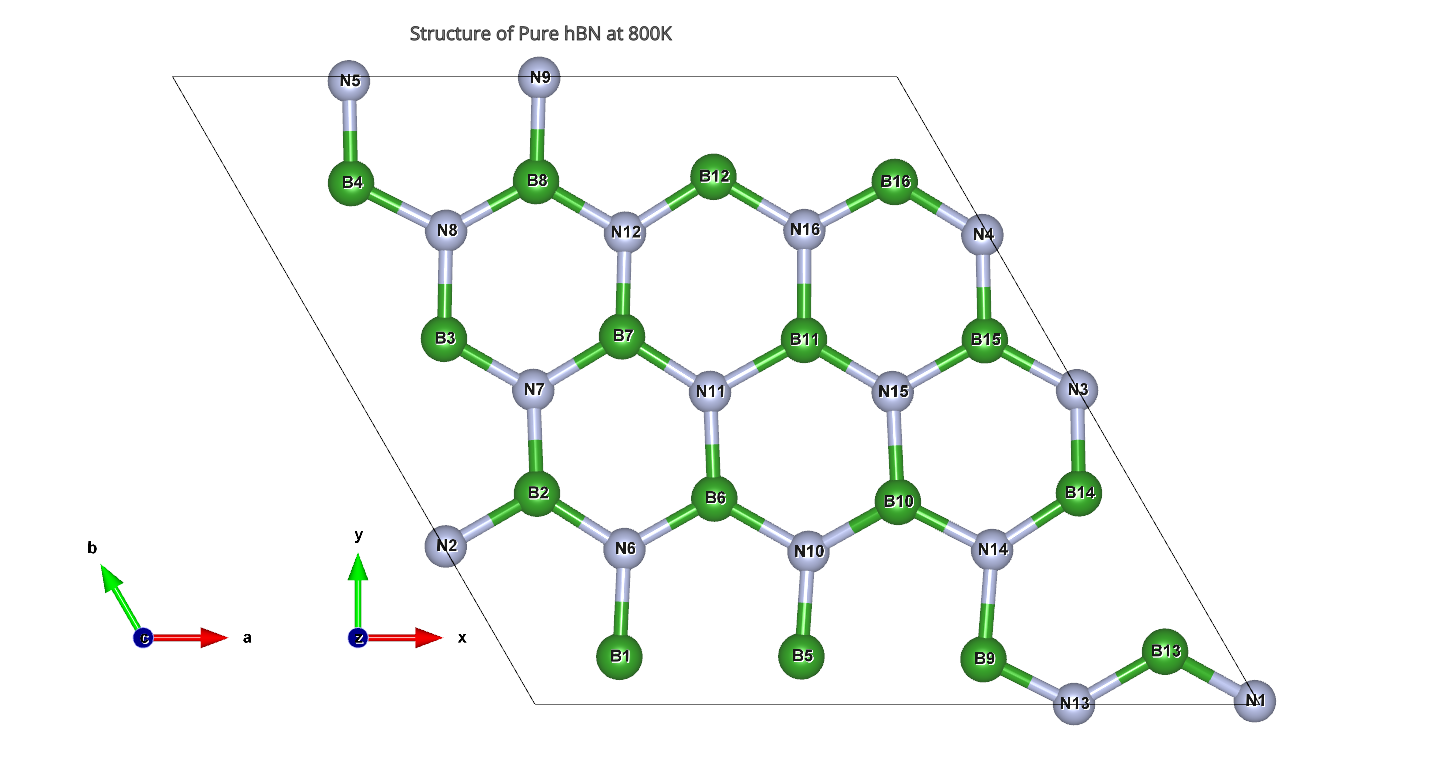
\includegraphics[width=0.49\linewidth]{gambar_hasil/hBN_pure_800K.png}\hfill
    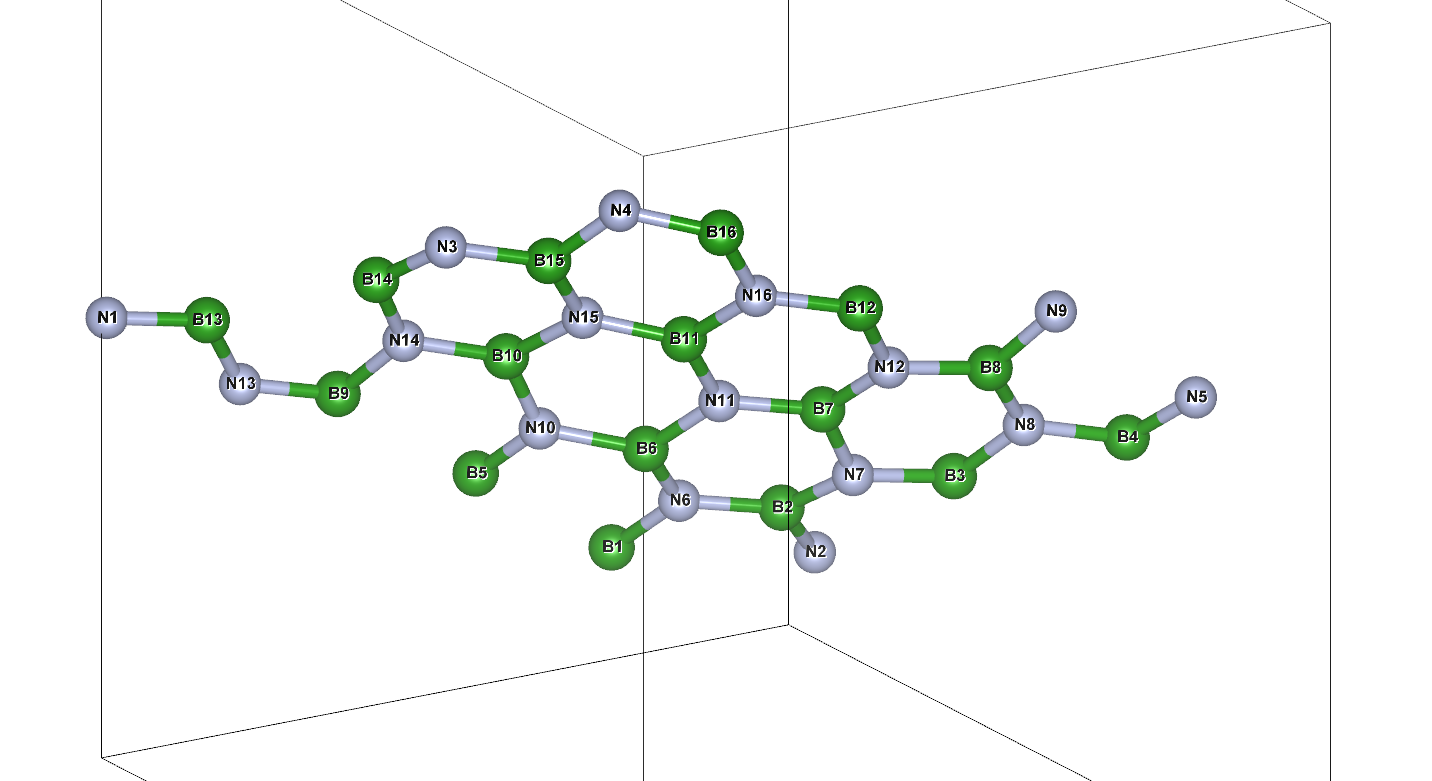
\includegraphics[width=0.49\linewidth]{hBN_pure_side_800K.png}
    \caption{Murni, 800 K}
    \label{subfig:md_pure_800k}
  \end{subfigure}
  \vspace{1em}
  \begin{subfigure}{\textwidth}
    \centering
    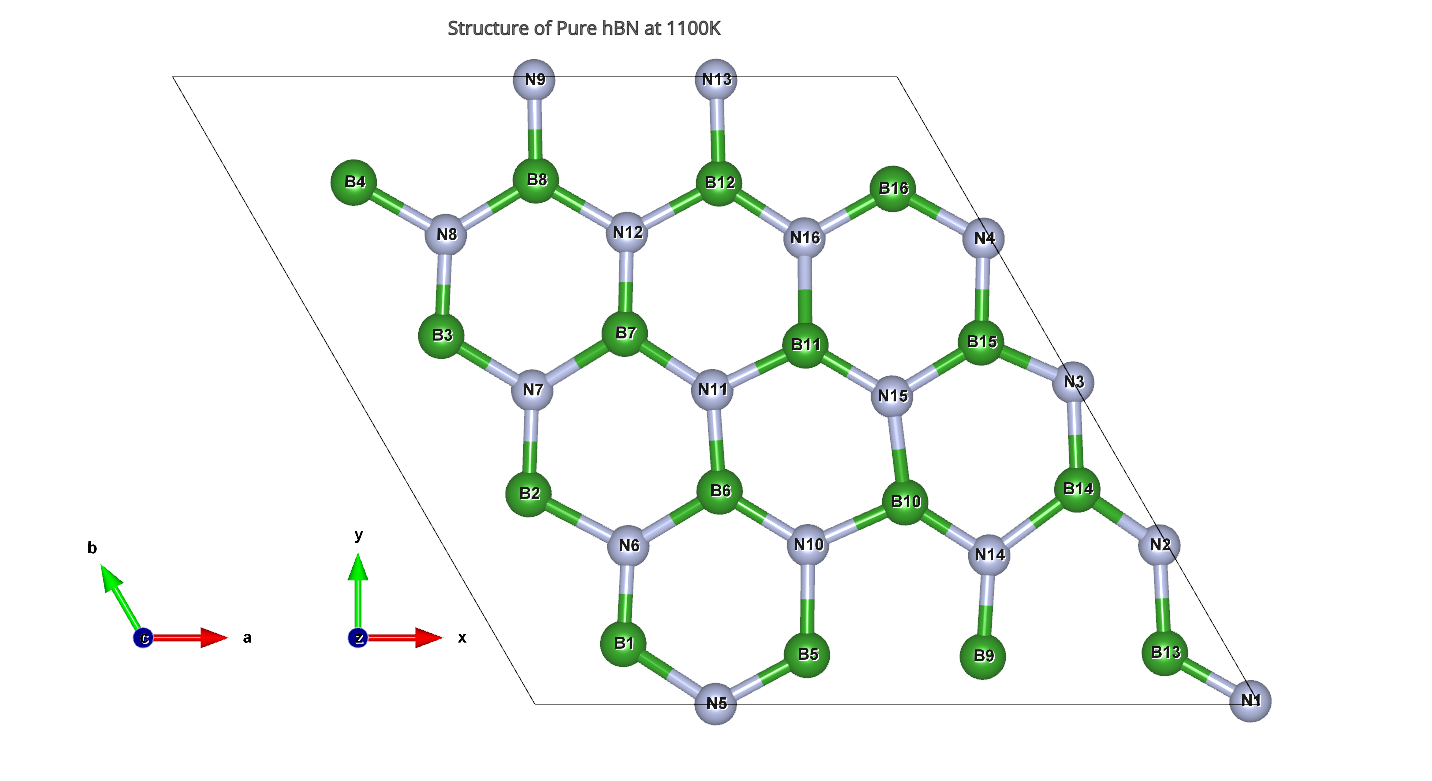
\includegraphics[width=0.49\linewidth]{gambar_hasil/hBN_pure_1100K.png}\hfill
    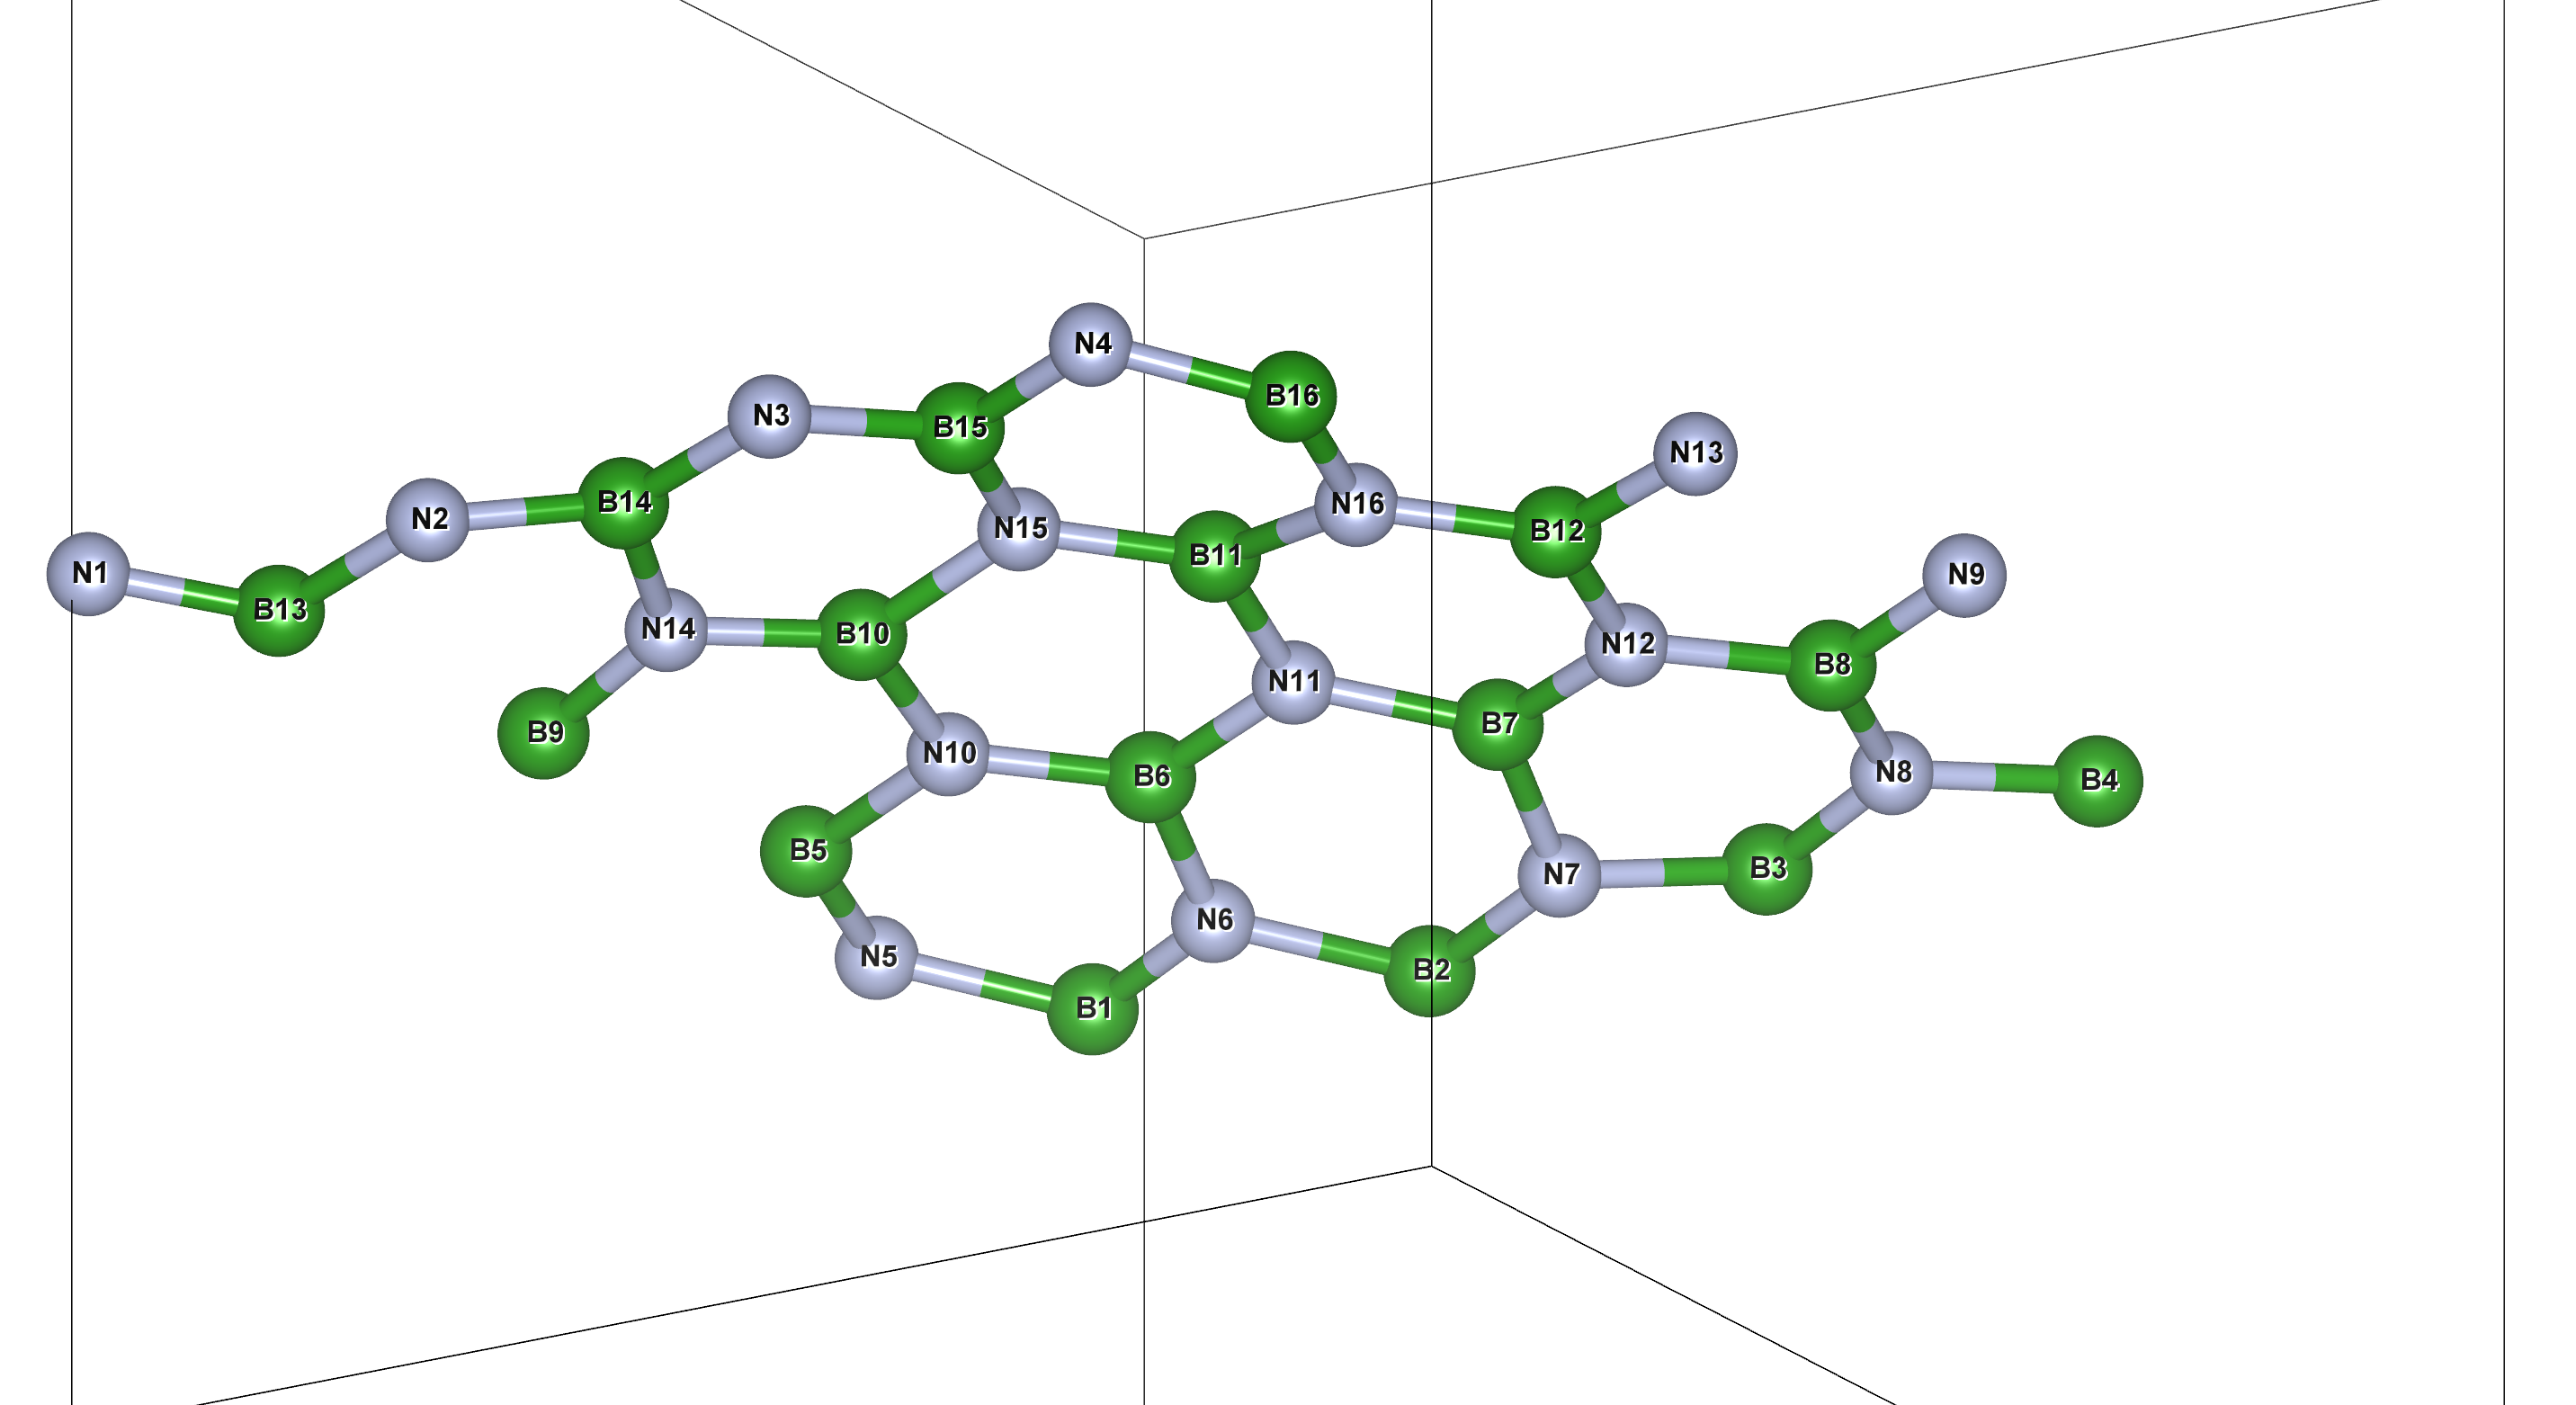
\includegraphics[width=0.49\linewidth]{gambar_hasil/hBN_pure_side_1100K.png}
    \caption{Murni, 1100 K}
    \label{subfig:md_pure_1100k}
  \end{subfigure}
  \vspace{1em}
  \begin{subfigure}{\textwidth}
    \centering
    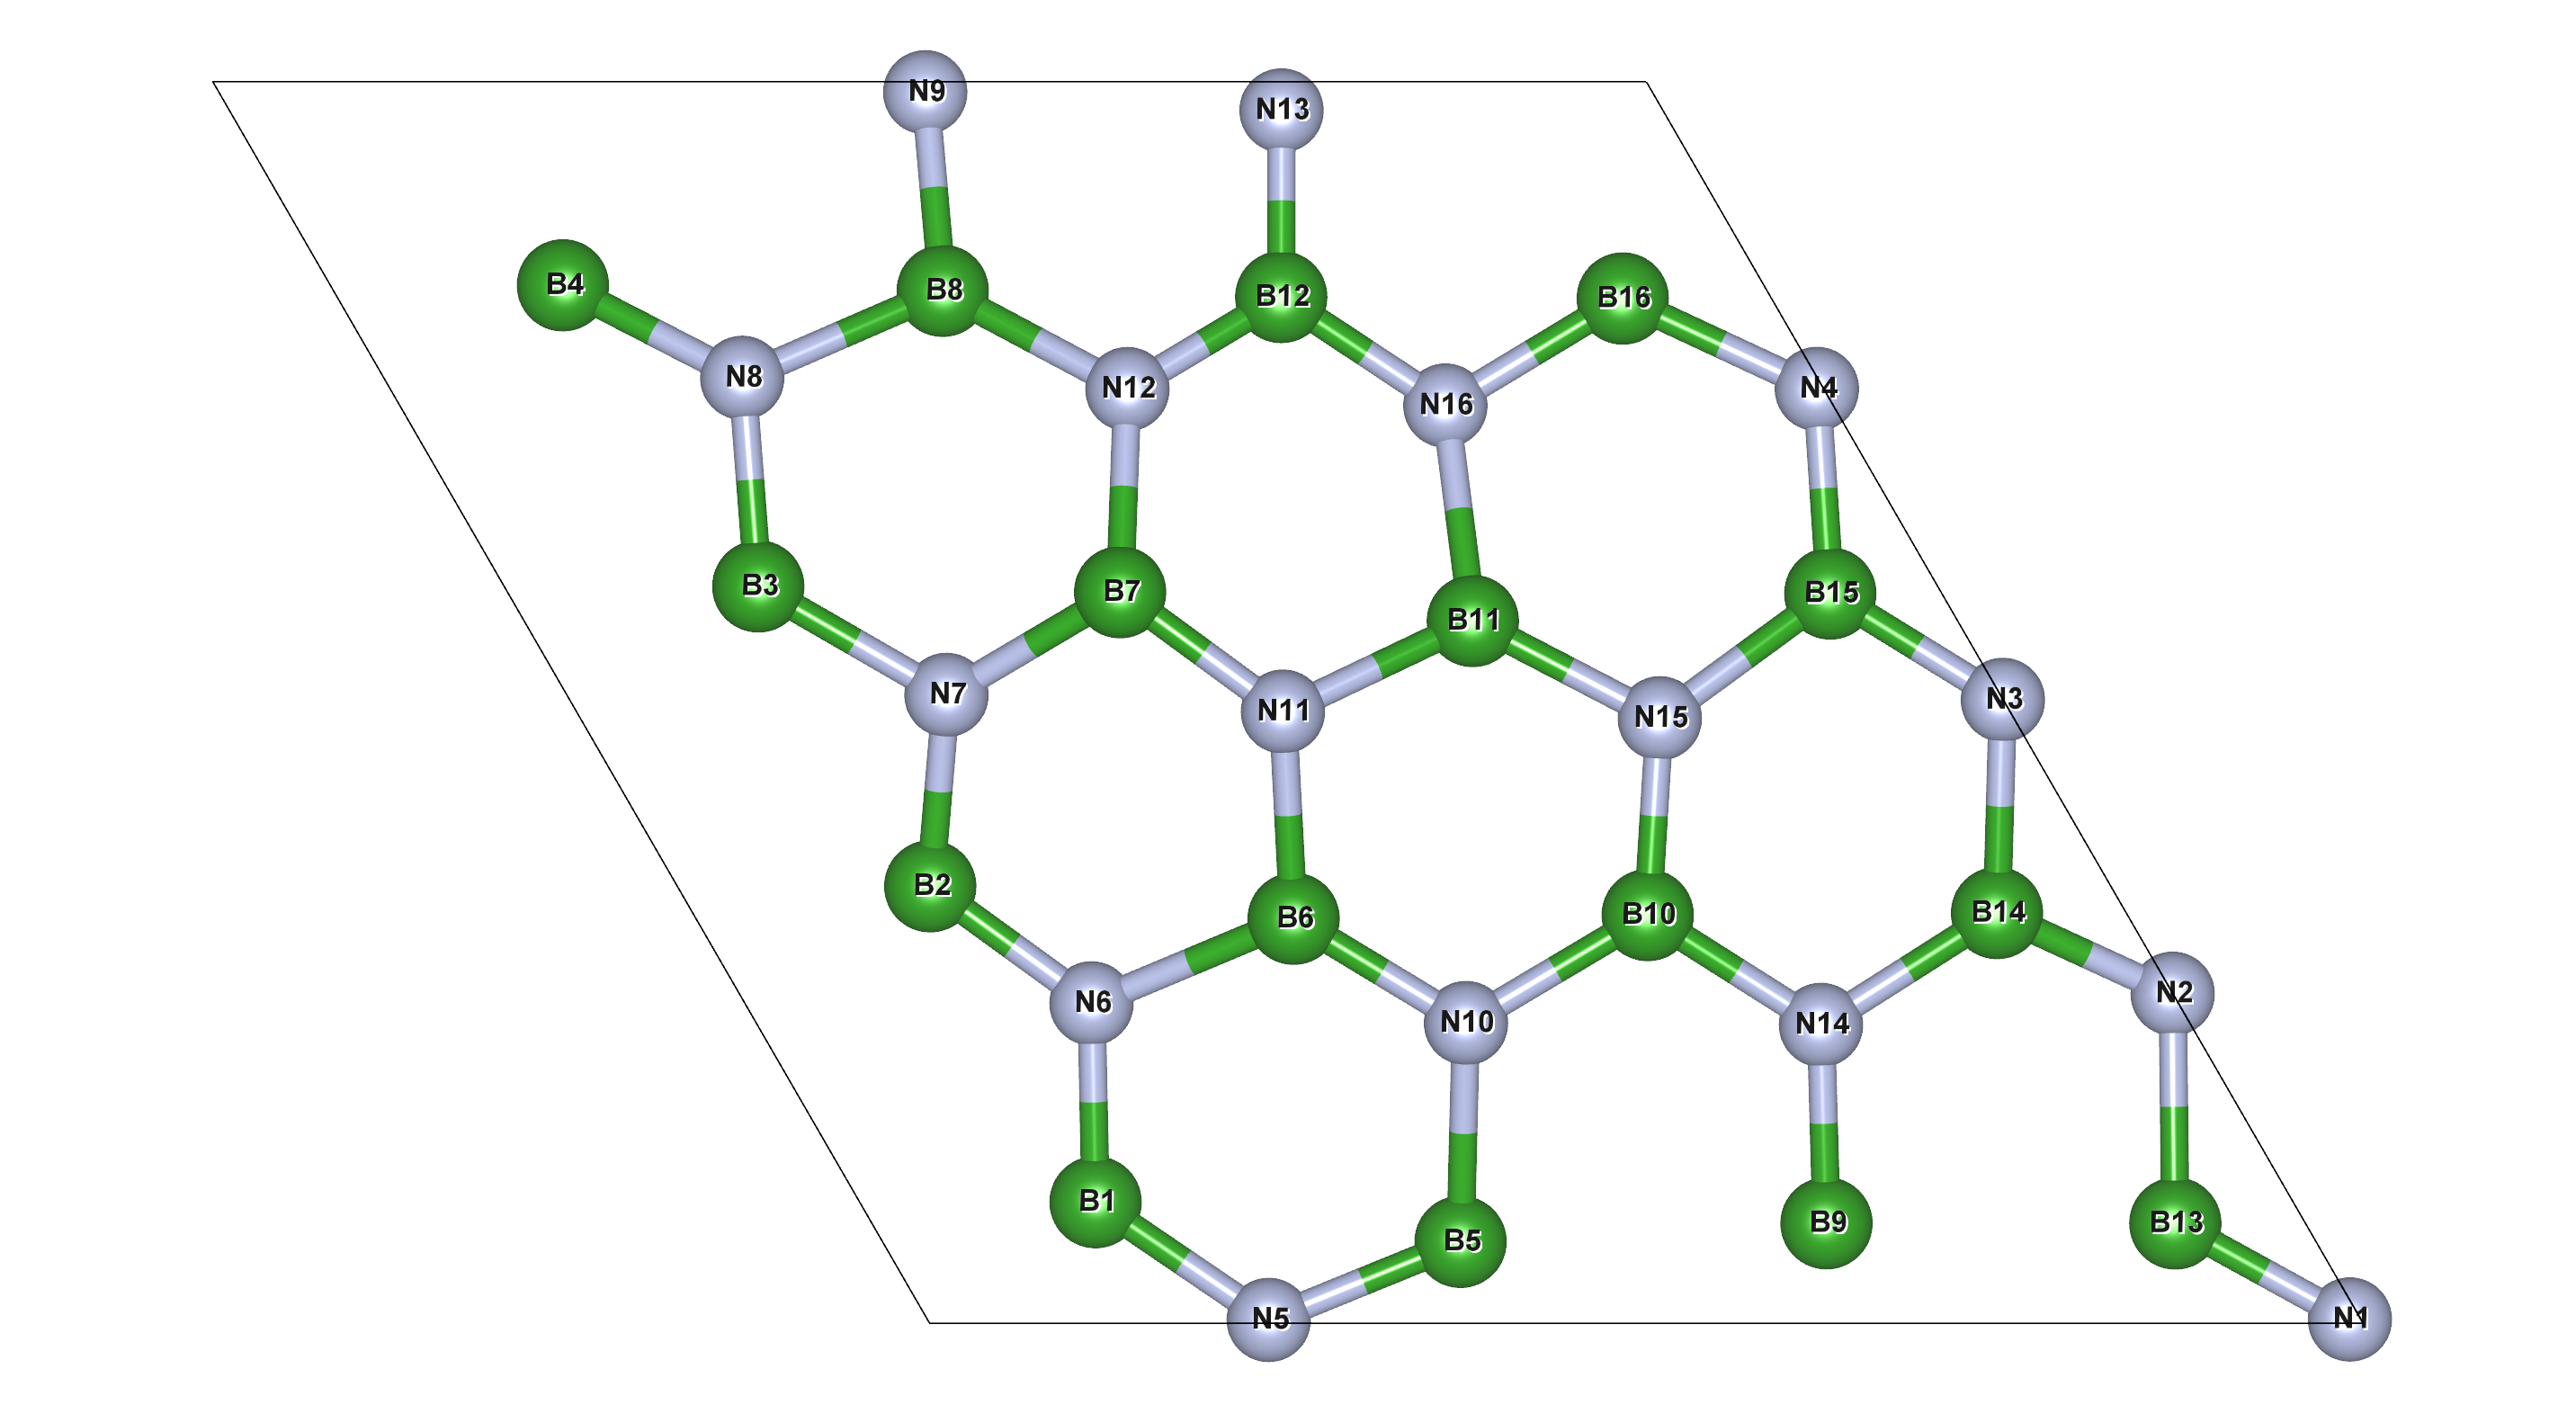
\includegraphics[width=0.49\linewidth]{gambar_hasil/hBN_pure_1225K.png}\hfill
    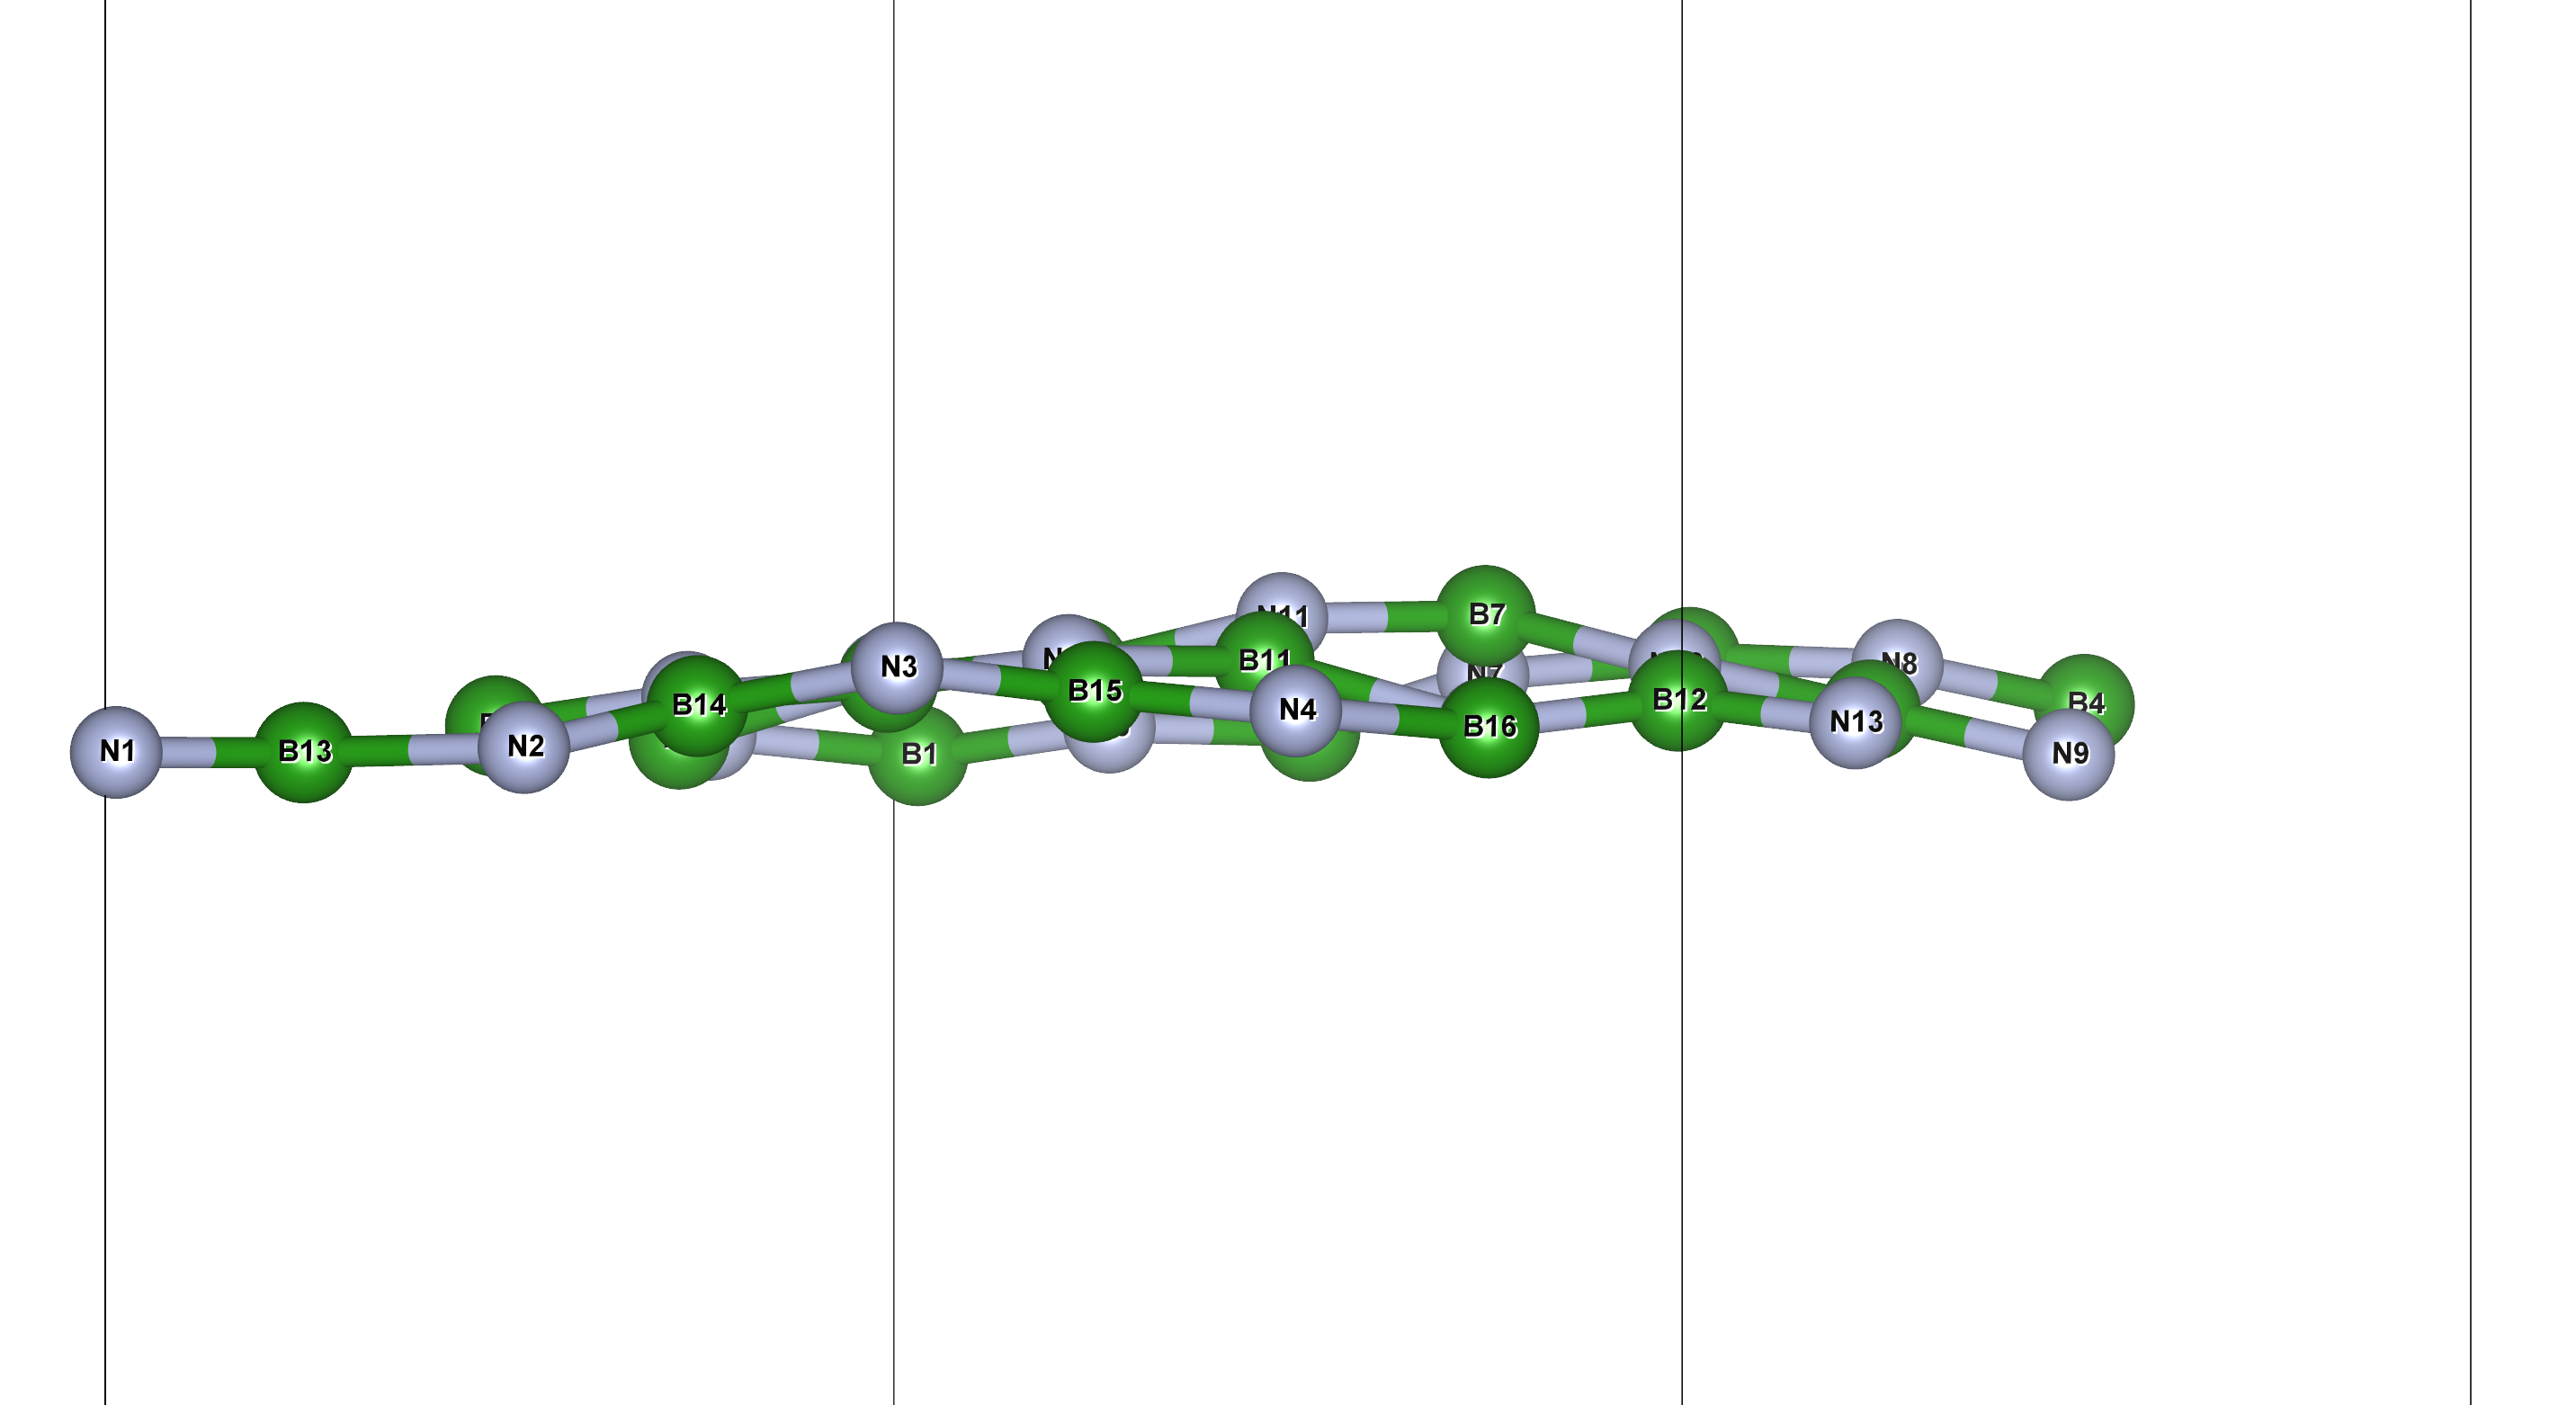
\includegraphics[width=0.49\linewidth]{gambar_hasil/hBN_pure_side_1225K.png}
    \caption{Murni, 1225 K}
    \label{subfig:md_pure_1225k}
  \end{subfigure}
\end{figure}

% --- Bagian 2: Cacat N_B (lanjutan) ---
\begin{figure}[htbp]\ContinuedFloat
  \centering
  \begin{subfigure}{\textwidth}
    \centering
    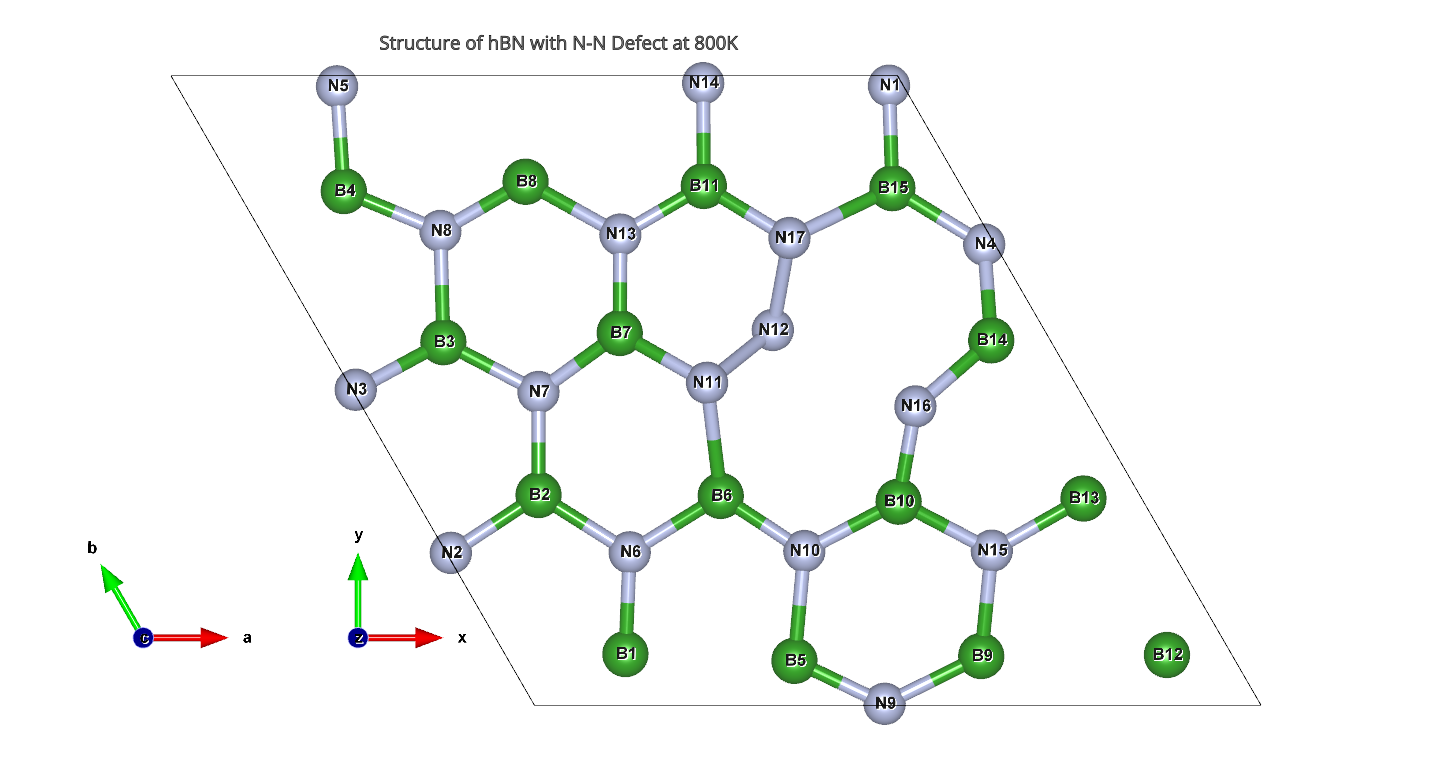
\includegraphics[width=0.49\linewidth]{gambar_hasil/hBN_NN_800K.png}\hfill
    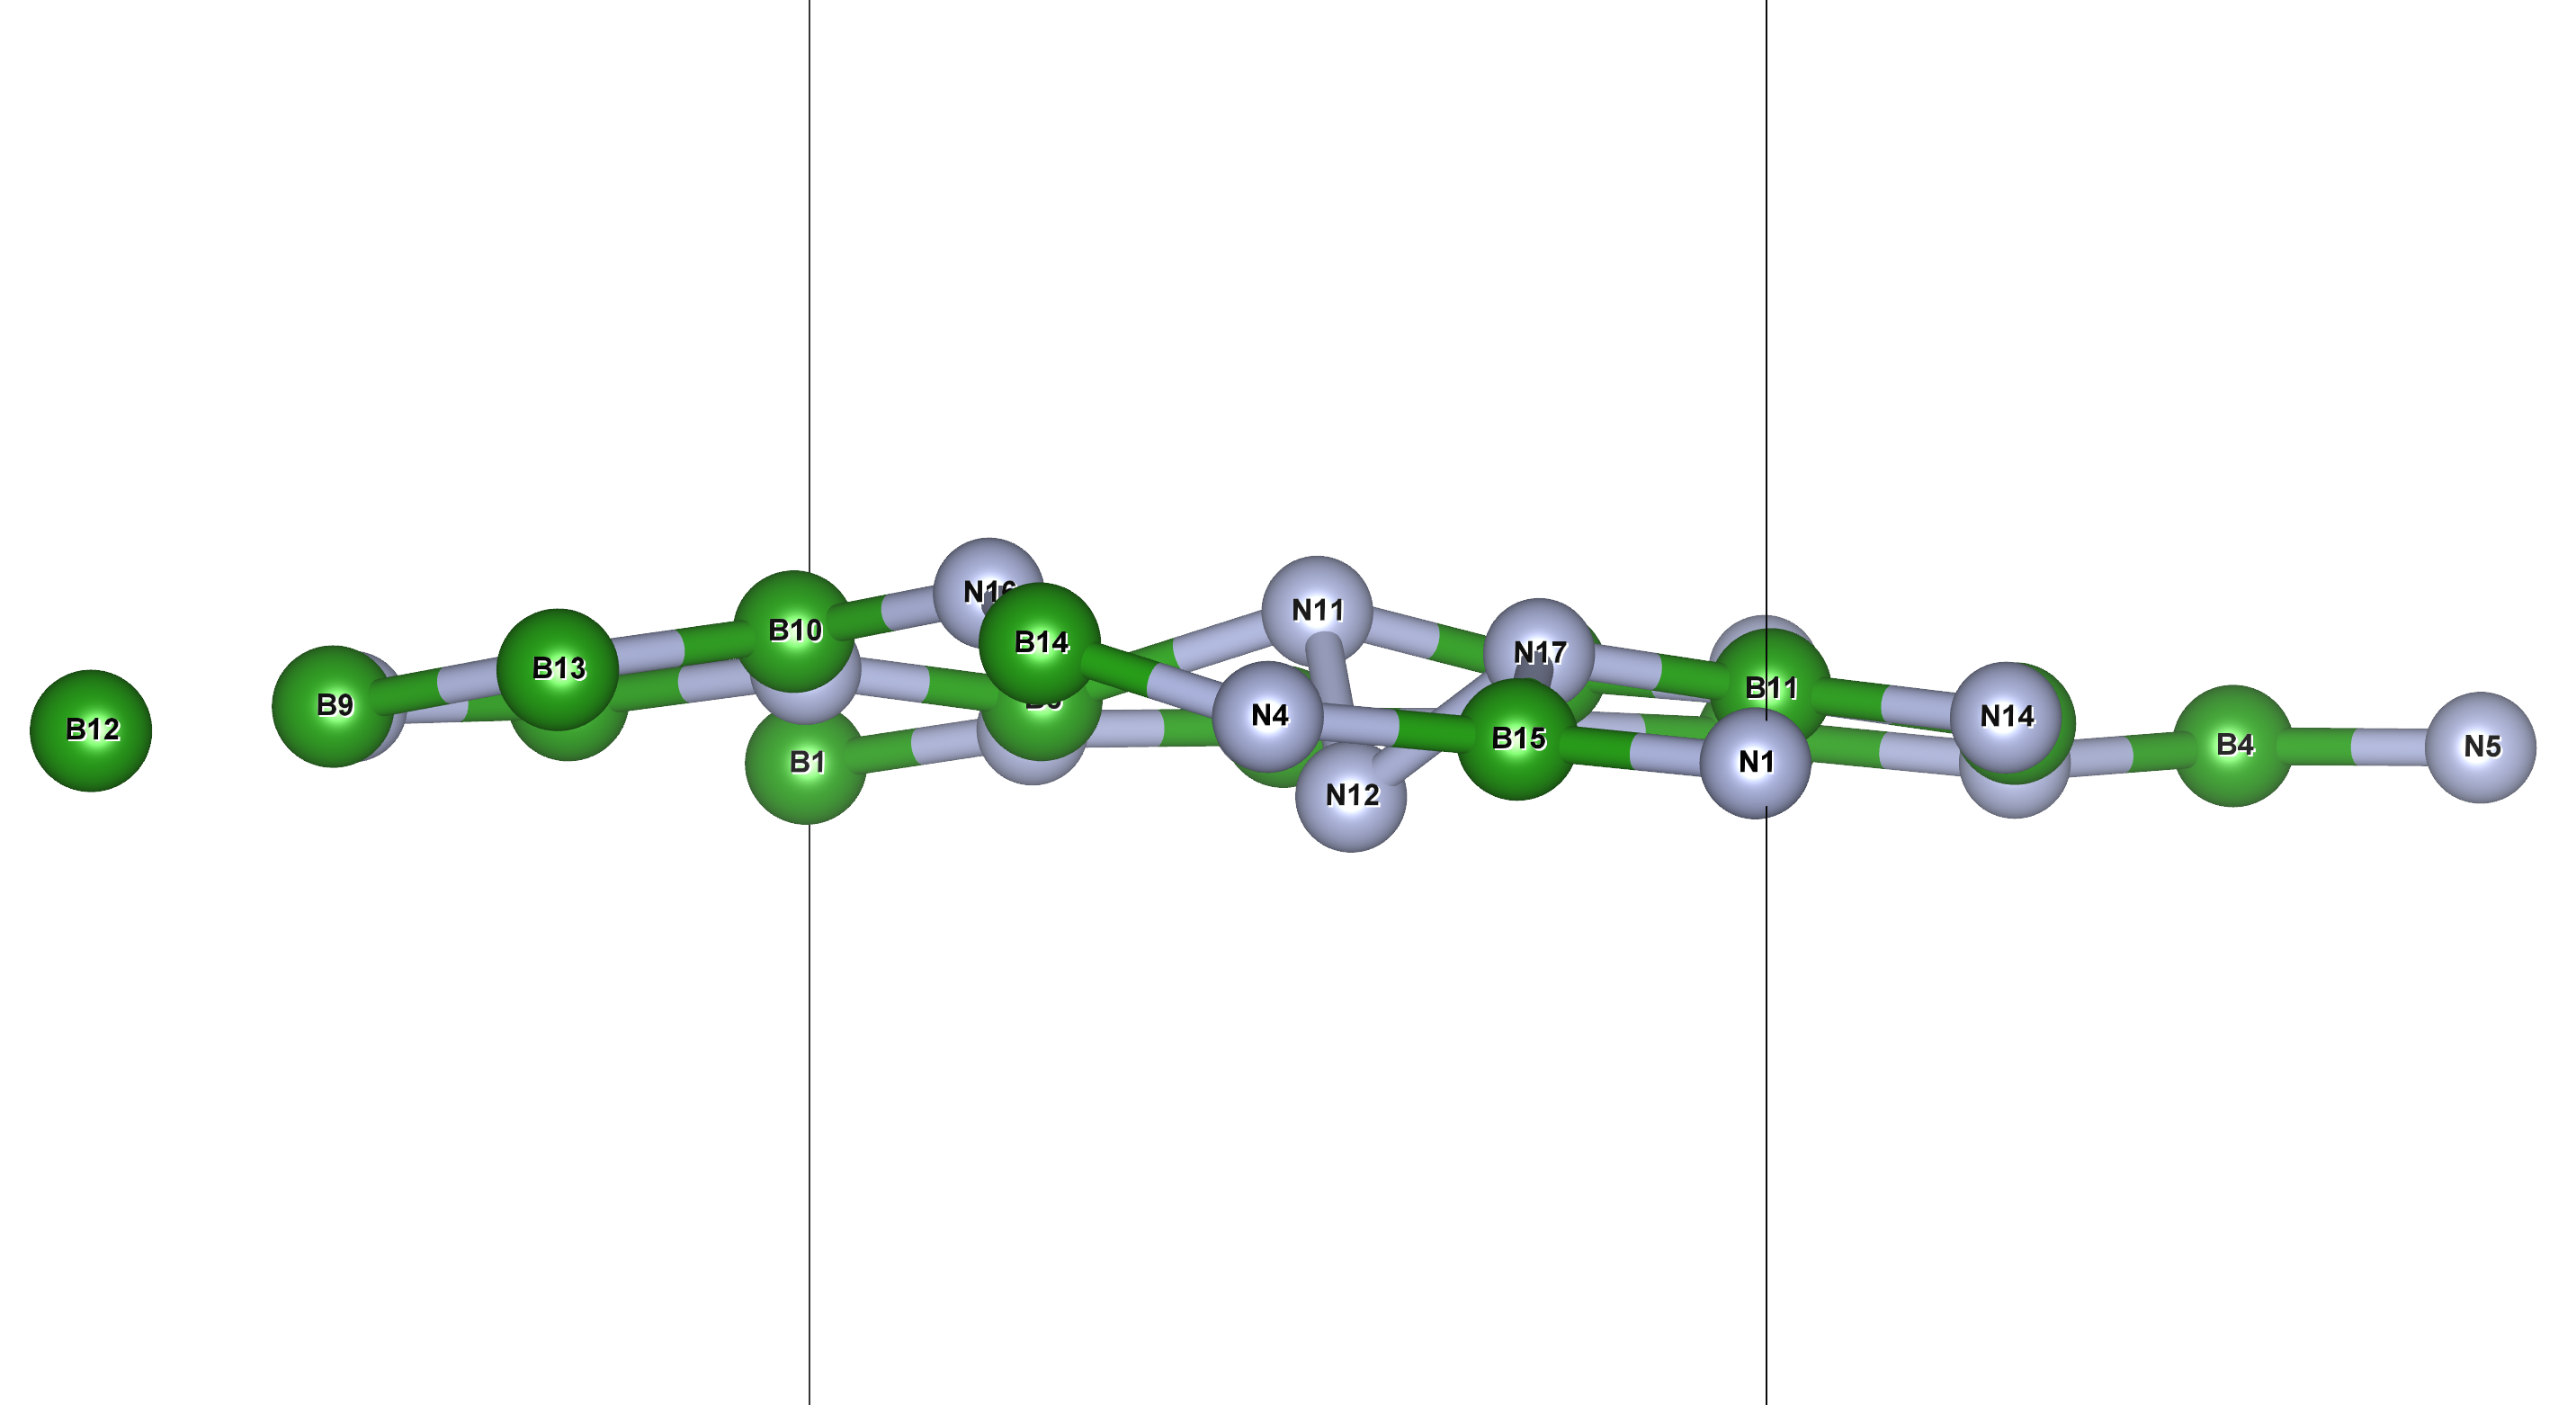
\includegraphics[width=0.49\linewidth]{gambar_hasil/hBN_NN_side_800K.png}
    \caption{Cacat N\textsubscript{B}, 800 K}
    \label{subfig:md_nn_800k}
  \end{subfigure}
  \vspace{1em}
  \begin{subfigure}{\textwidth}
    \centering
    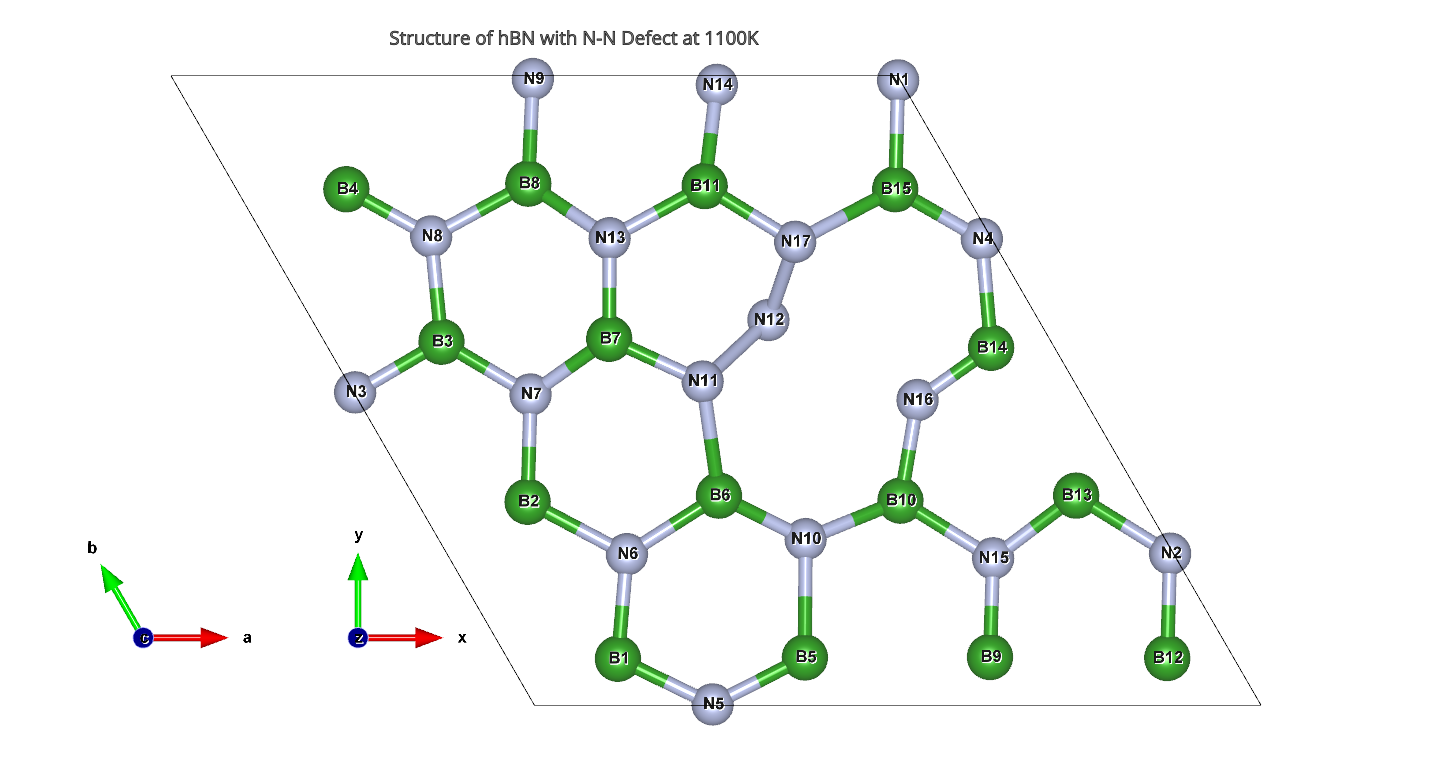
\includegraphics[width=0.49\linewidth]{gambar_hasil/hBN_NN_1100K.png}\hfill
    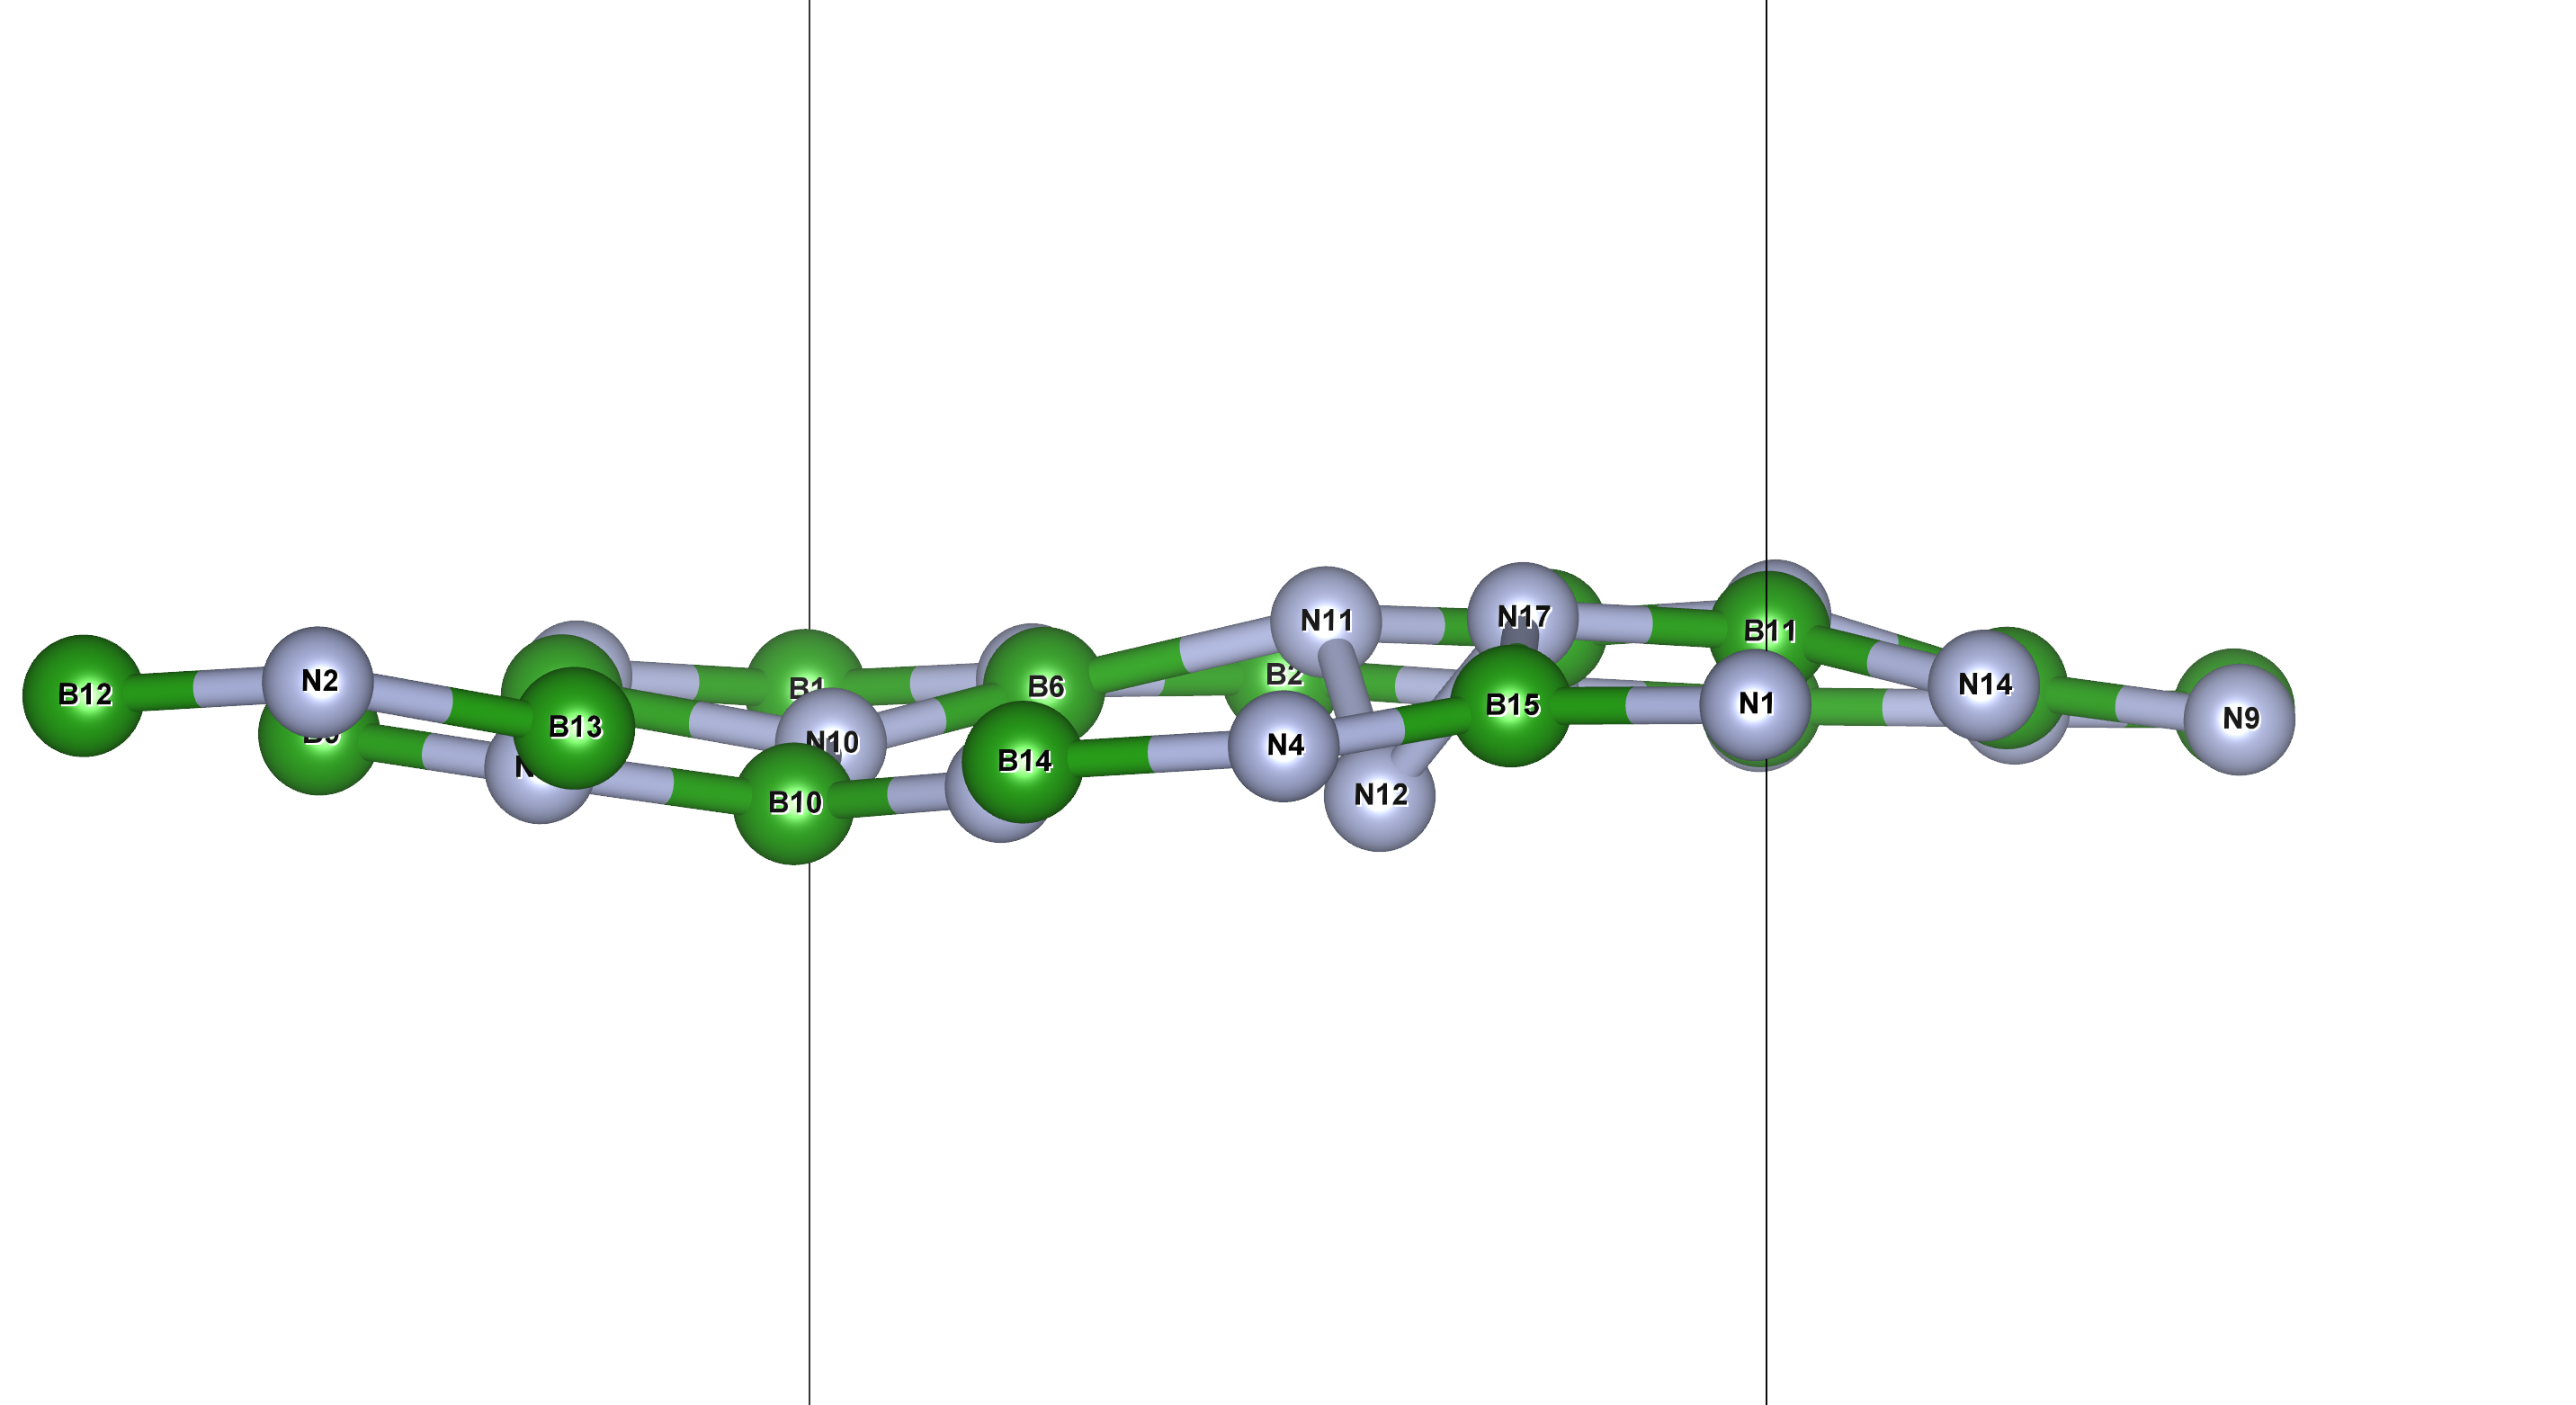
\includegraphics[width=0.49\linewidth]{gambar_hasil/hBN_NN_side_1100K.png}
    \caption{Cacat N\textsubscript{B}, 1100 K}
    \label{subfig:md_nn_1100k}
  \end{subfigure}
  \vspace{1em}
  \begin{subfigure}{\textwidth}
    \centering
    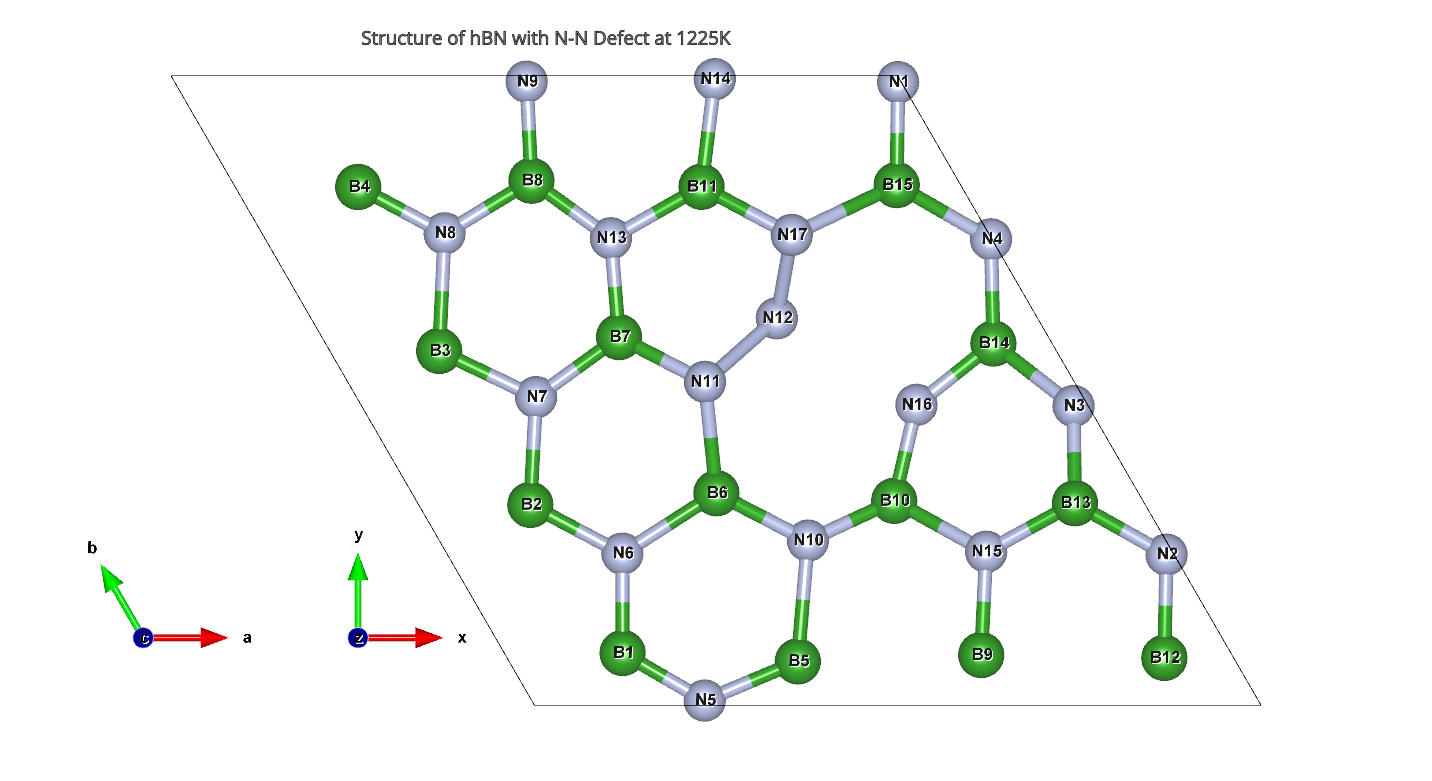
\includegraphics[width=0.49\linewidth]{gambar_hasil/hBN_NN_1225K.png}\hfill
    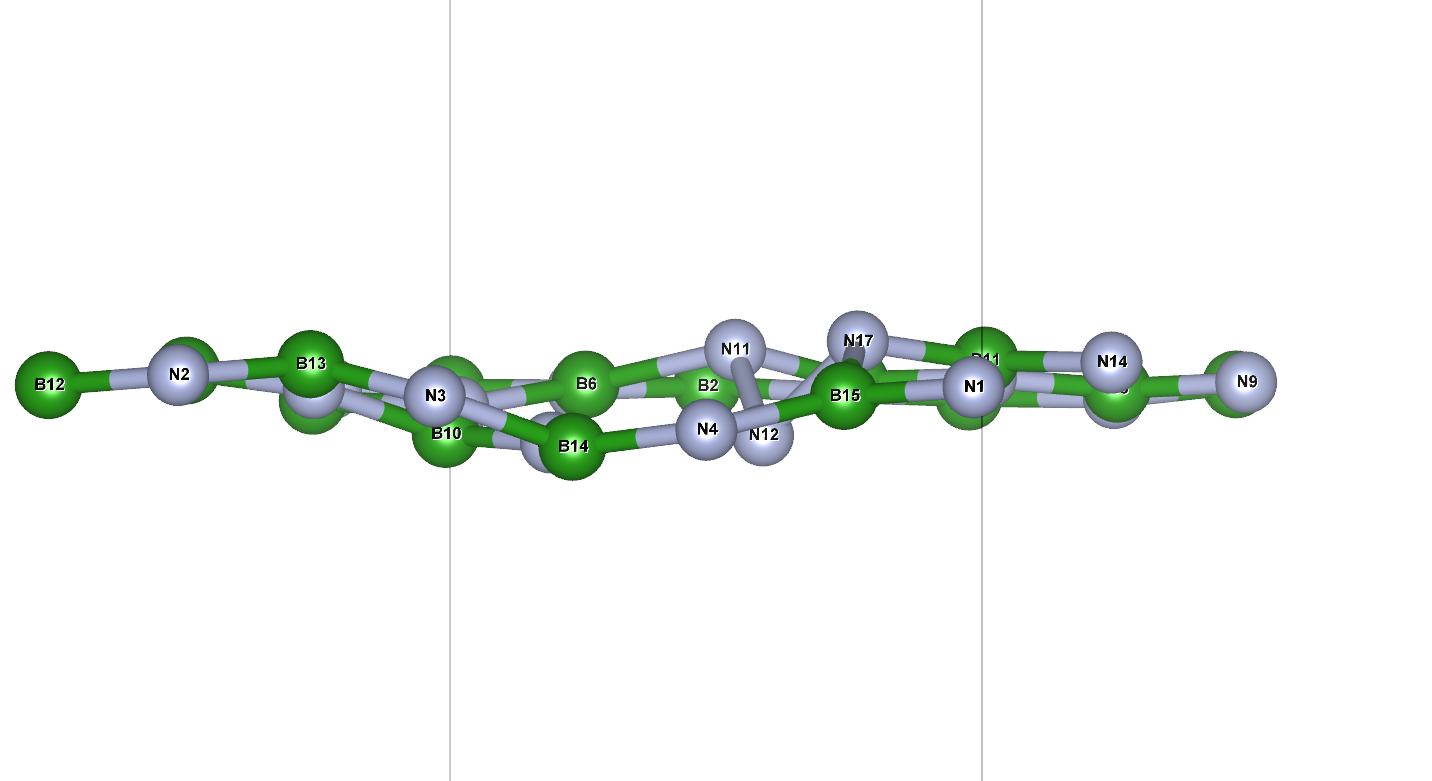
\includegraphics[width=0.49\linewidth]{gambar_hasil/hBN_NN_side_1225K.png}
    \caption{Cacat N\textsubscript{B}, 1225 K}
    \label{subfig:md_nn_1225k}
  \end{subfigure}
\end{figure}

% --- Bagian 3: Cacat B_N (lanjutan) ---
\begin{figure}[htbp]\ContinuedFloat
  \centering
  \begin{subfigure}{\textwidth}
    \centering
    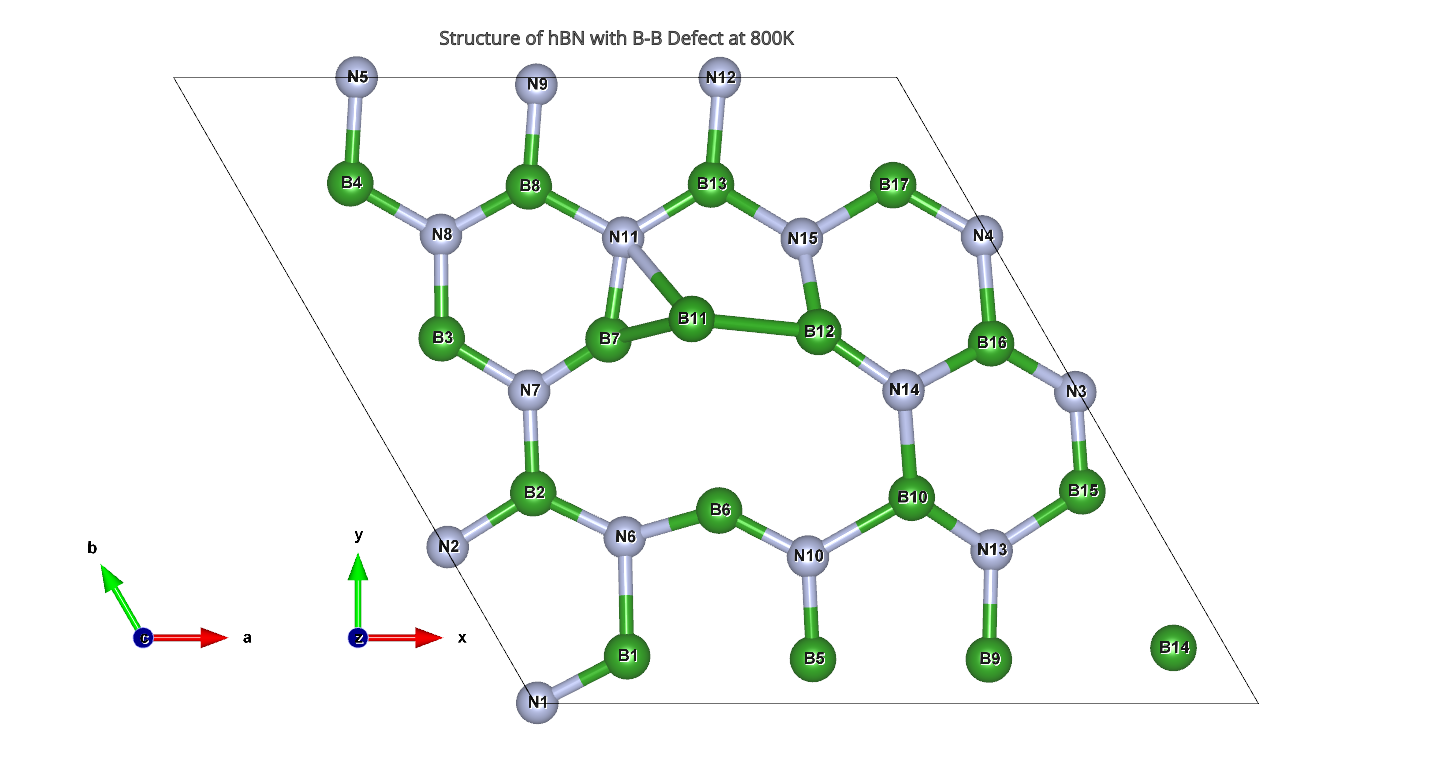
\includegraphics[width=0.49\linewidth]{gambar_hasil/hBN_BB_800K.png}\hfill
    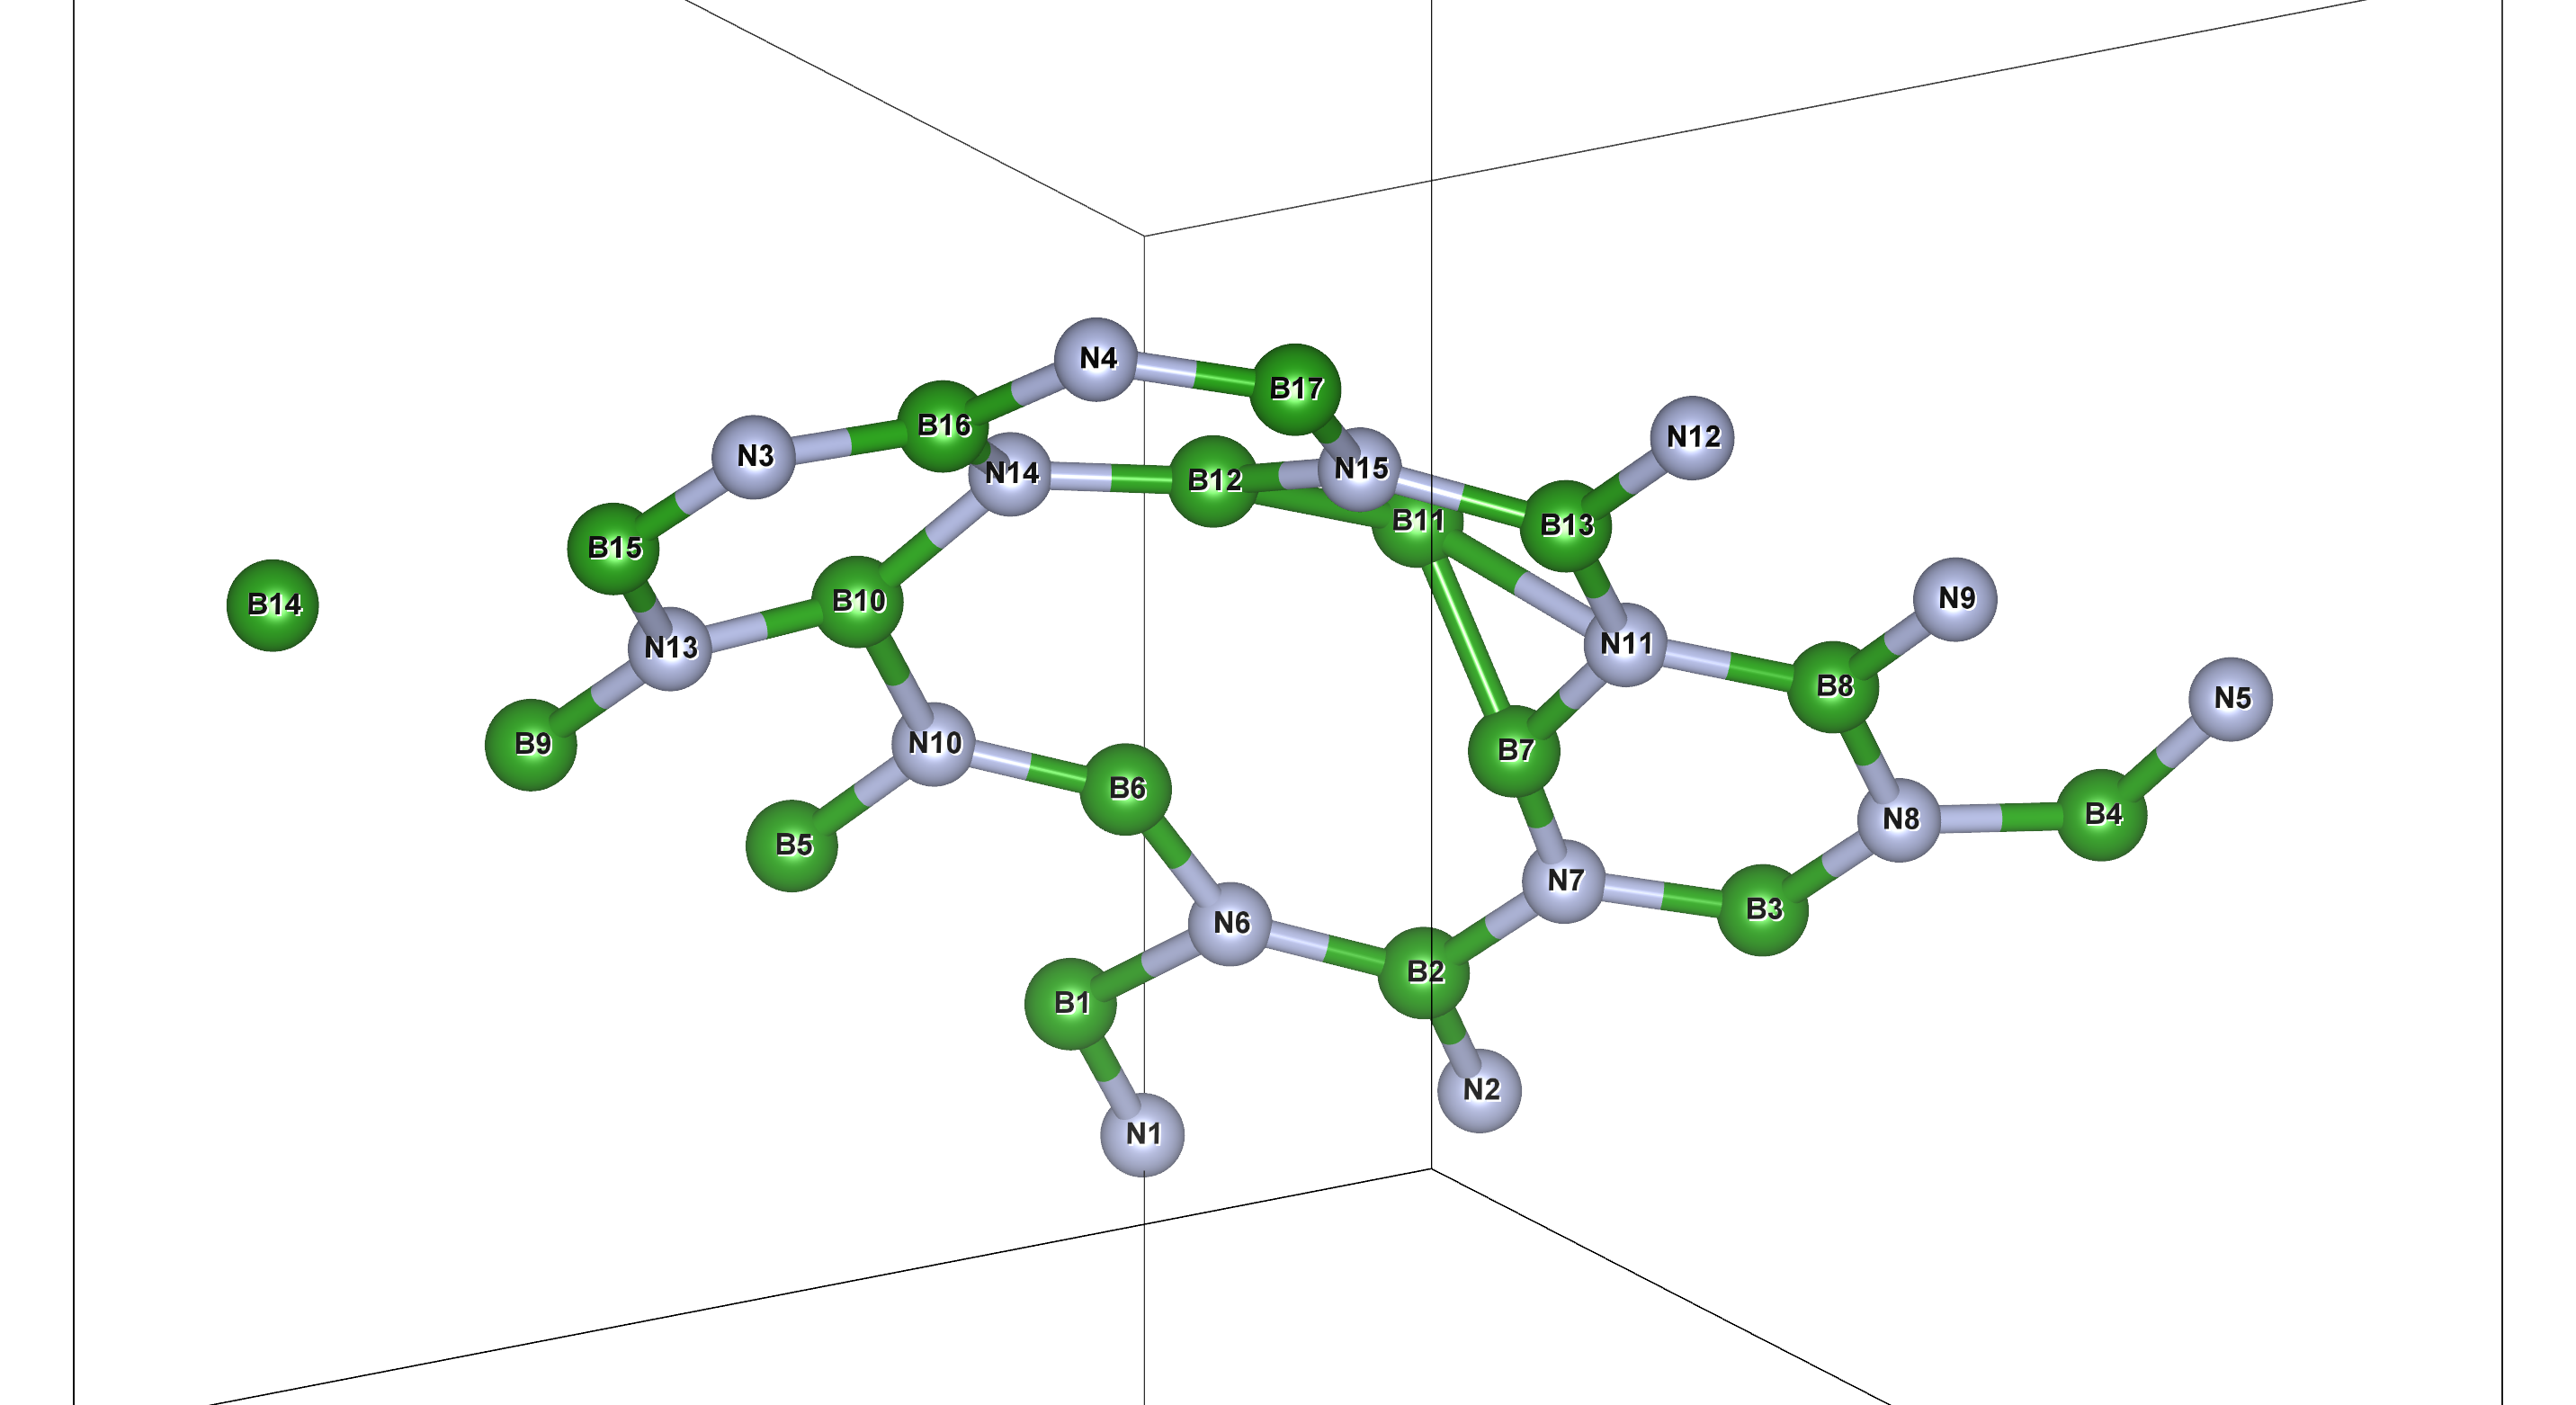
\includegraphics[width=0.49\linewidth]{gambar_hasil/hBN_BB_side_800K.png}
    \caption{Cacat B\textsubscript{N}, 800 K}
    \label{subfig:md_bb_800k}
  \end{subfigure}
  \vspace{1em}
  \begin{subfigure}{\textwidth}
    \centering
    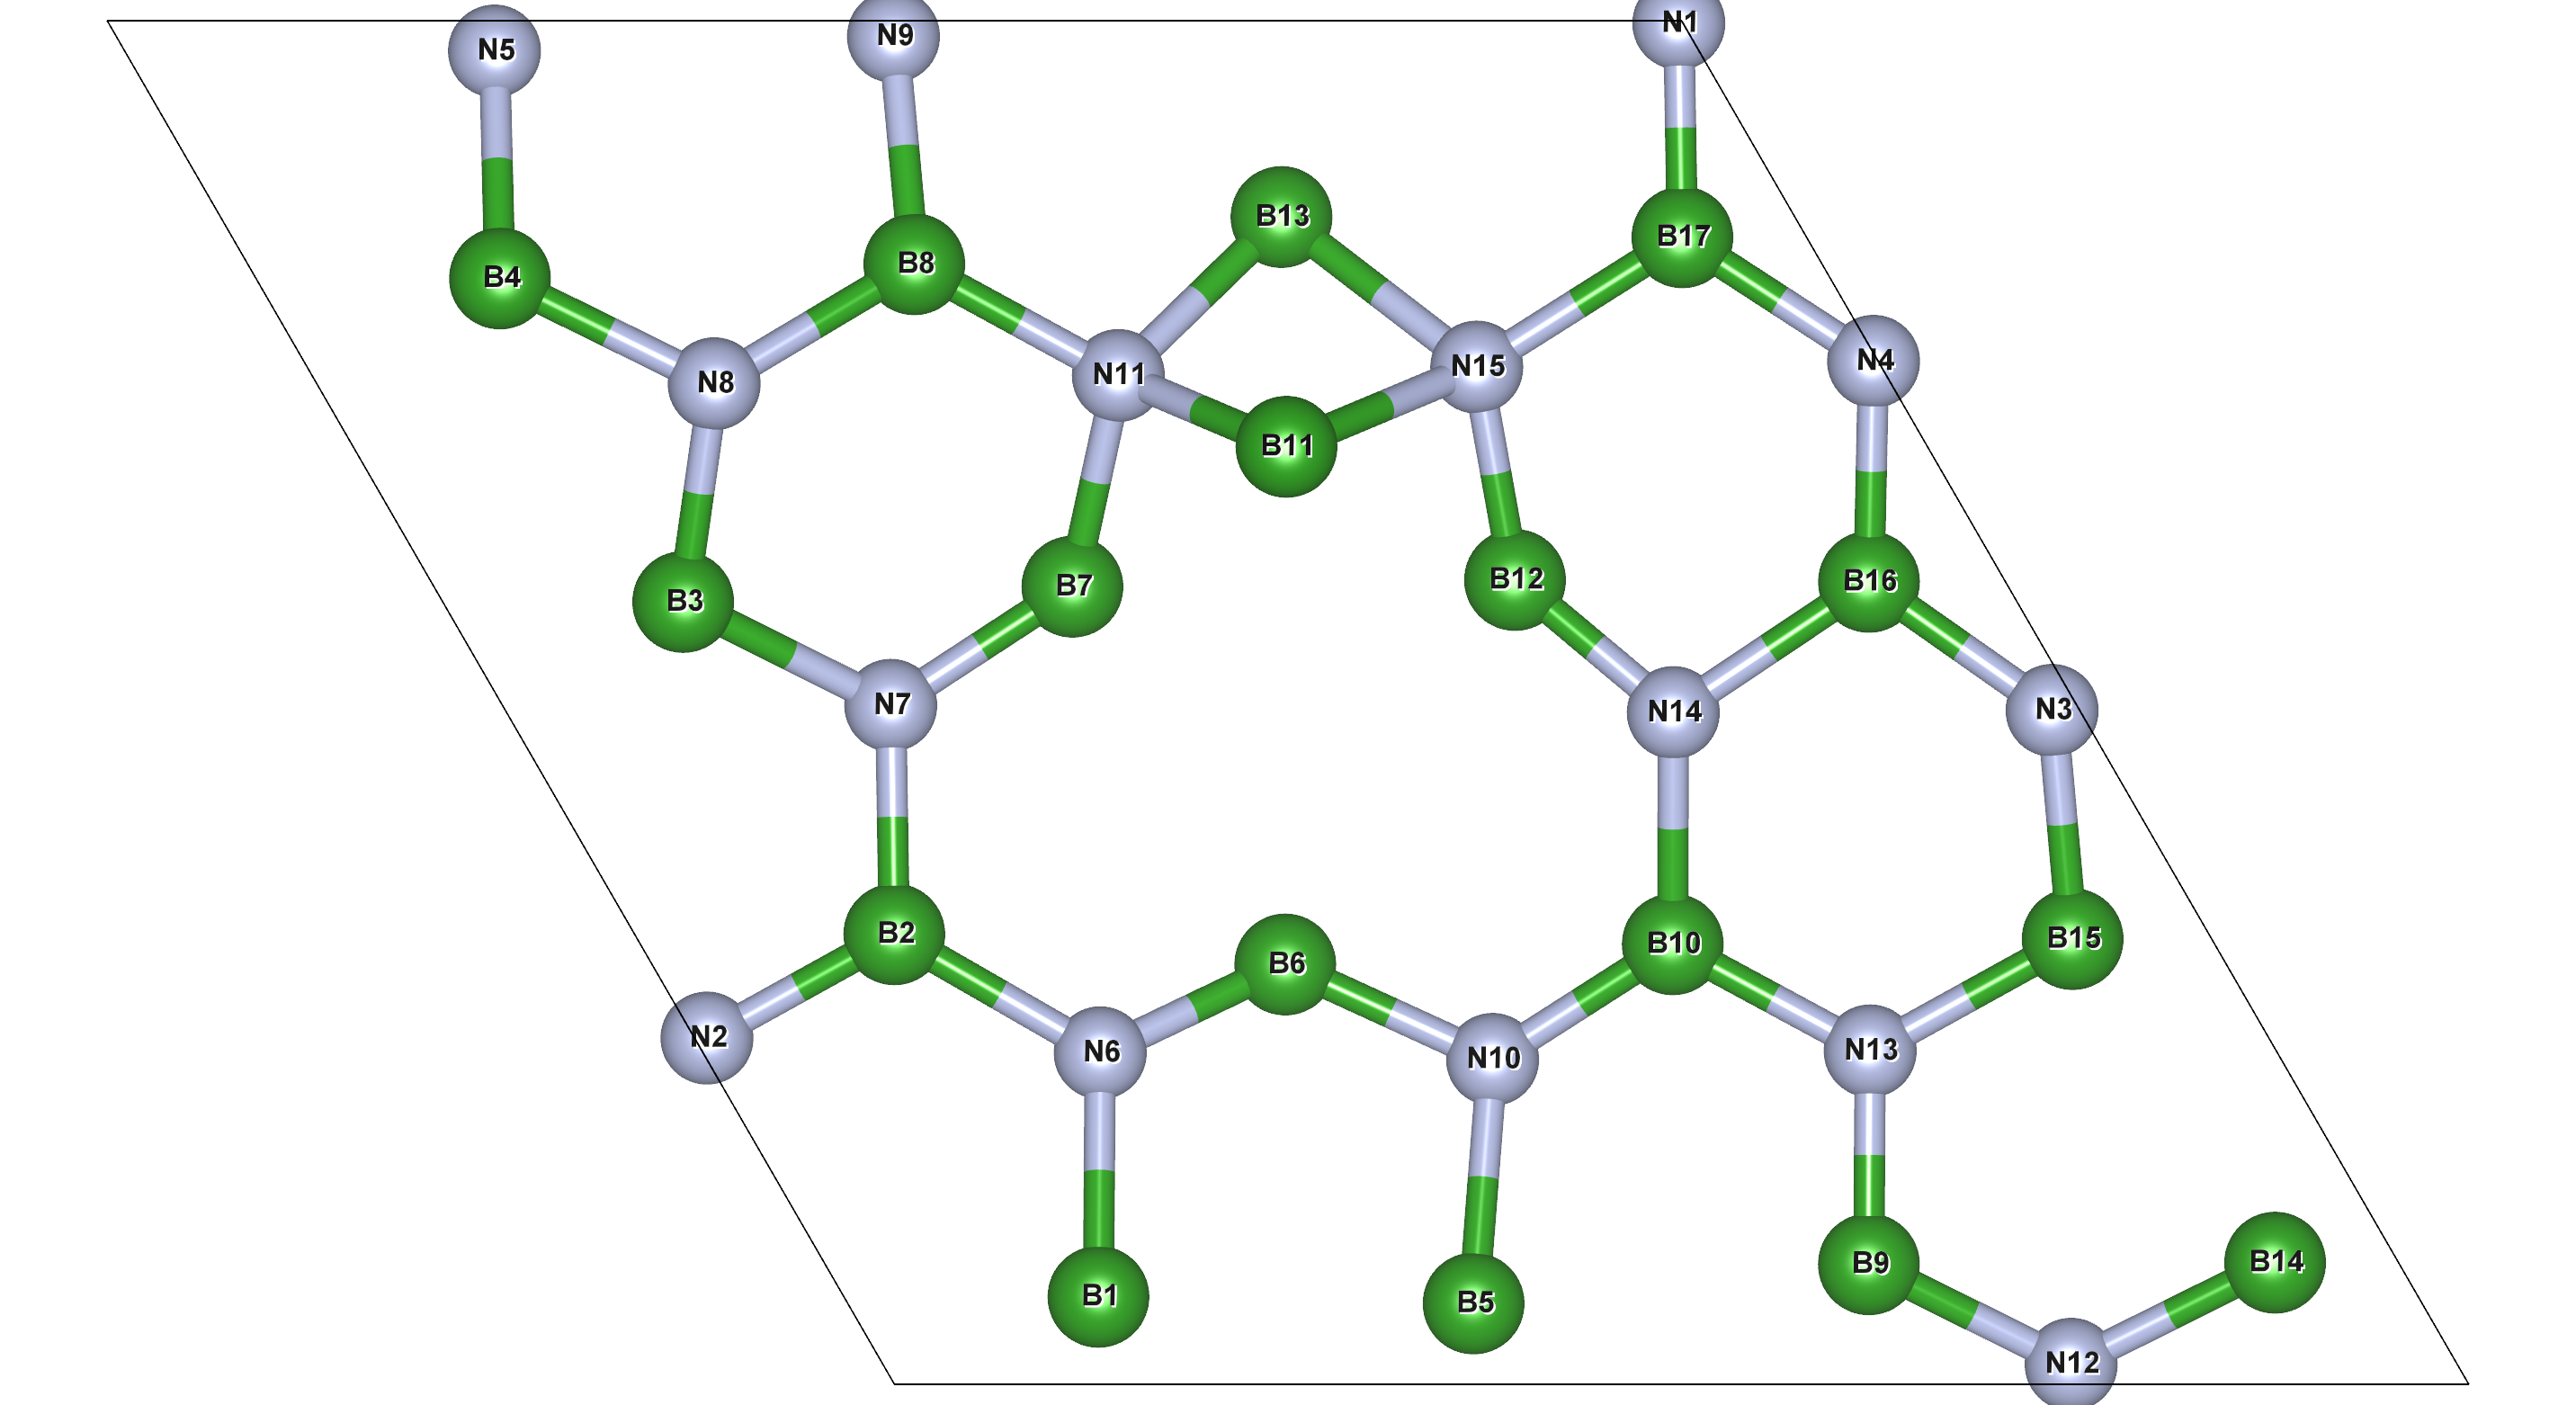
\includegraphics[width=0.49\linewidth]{gambar_hasil/hBN_BB_1100K.png}\hfill
    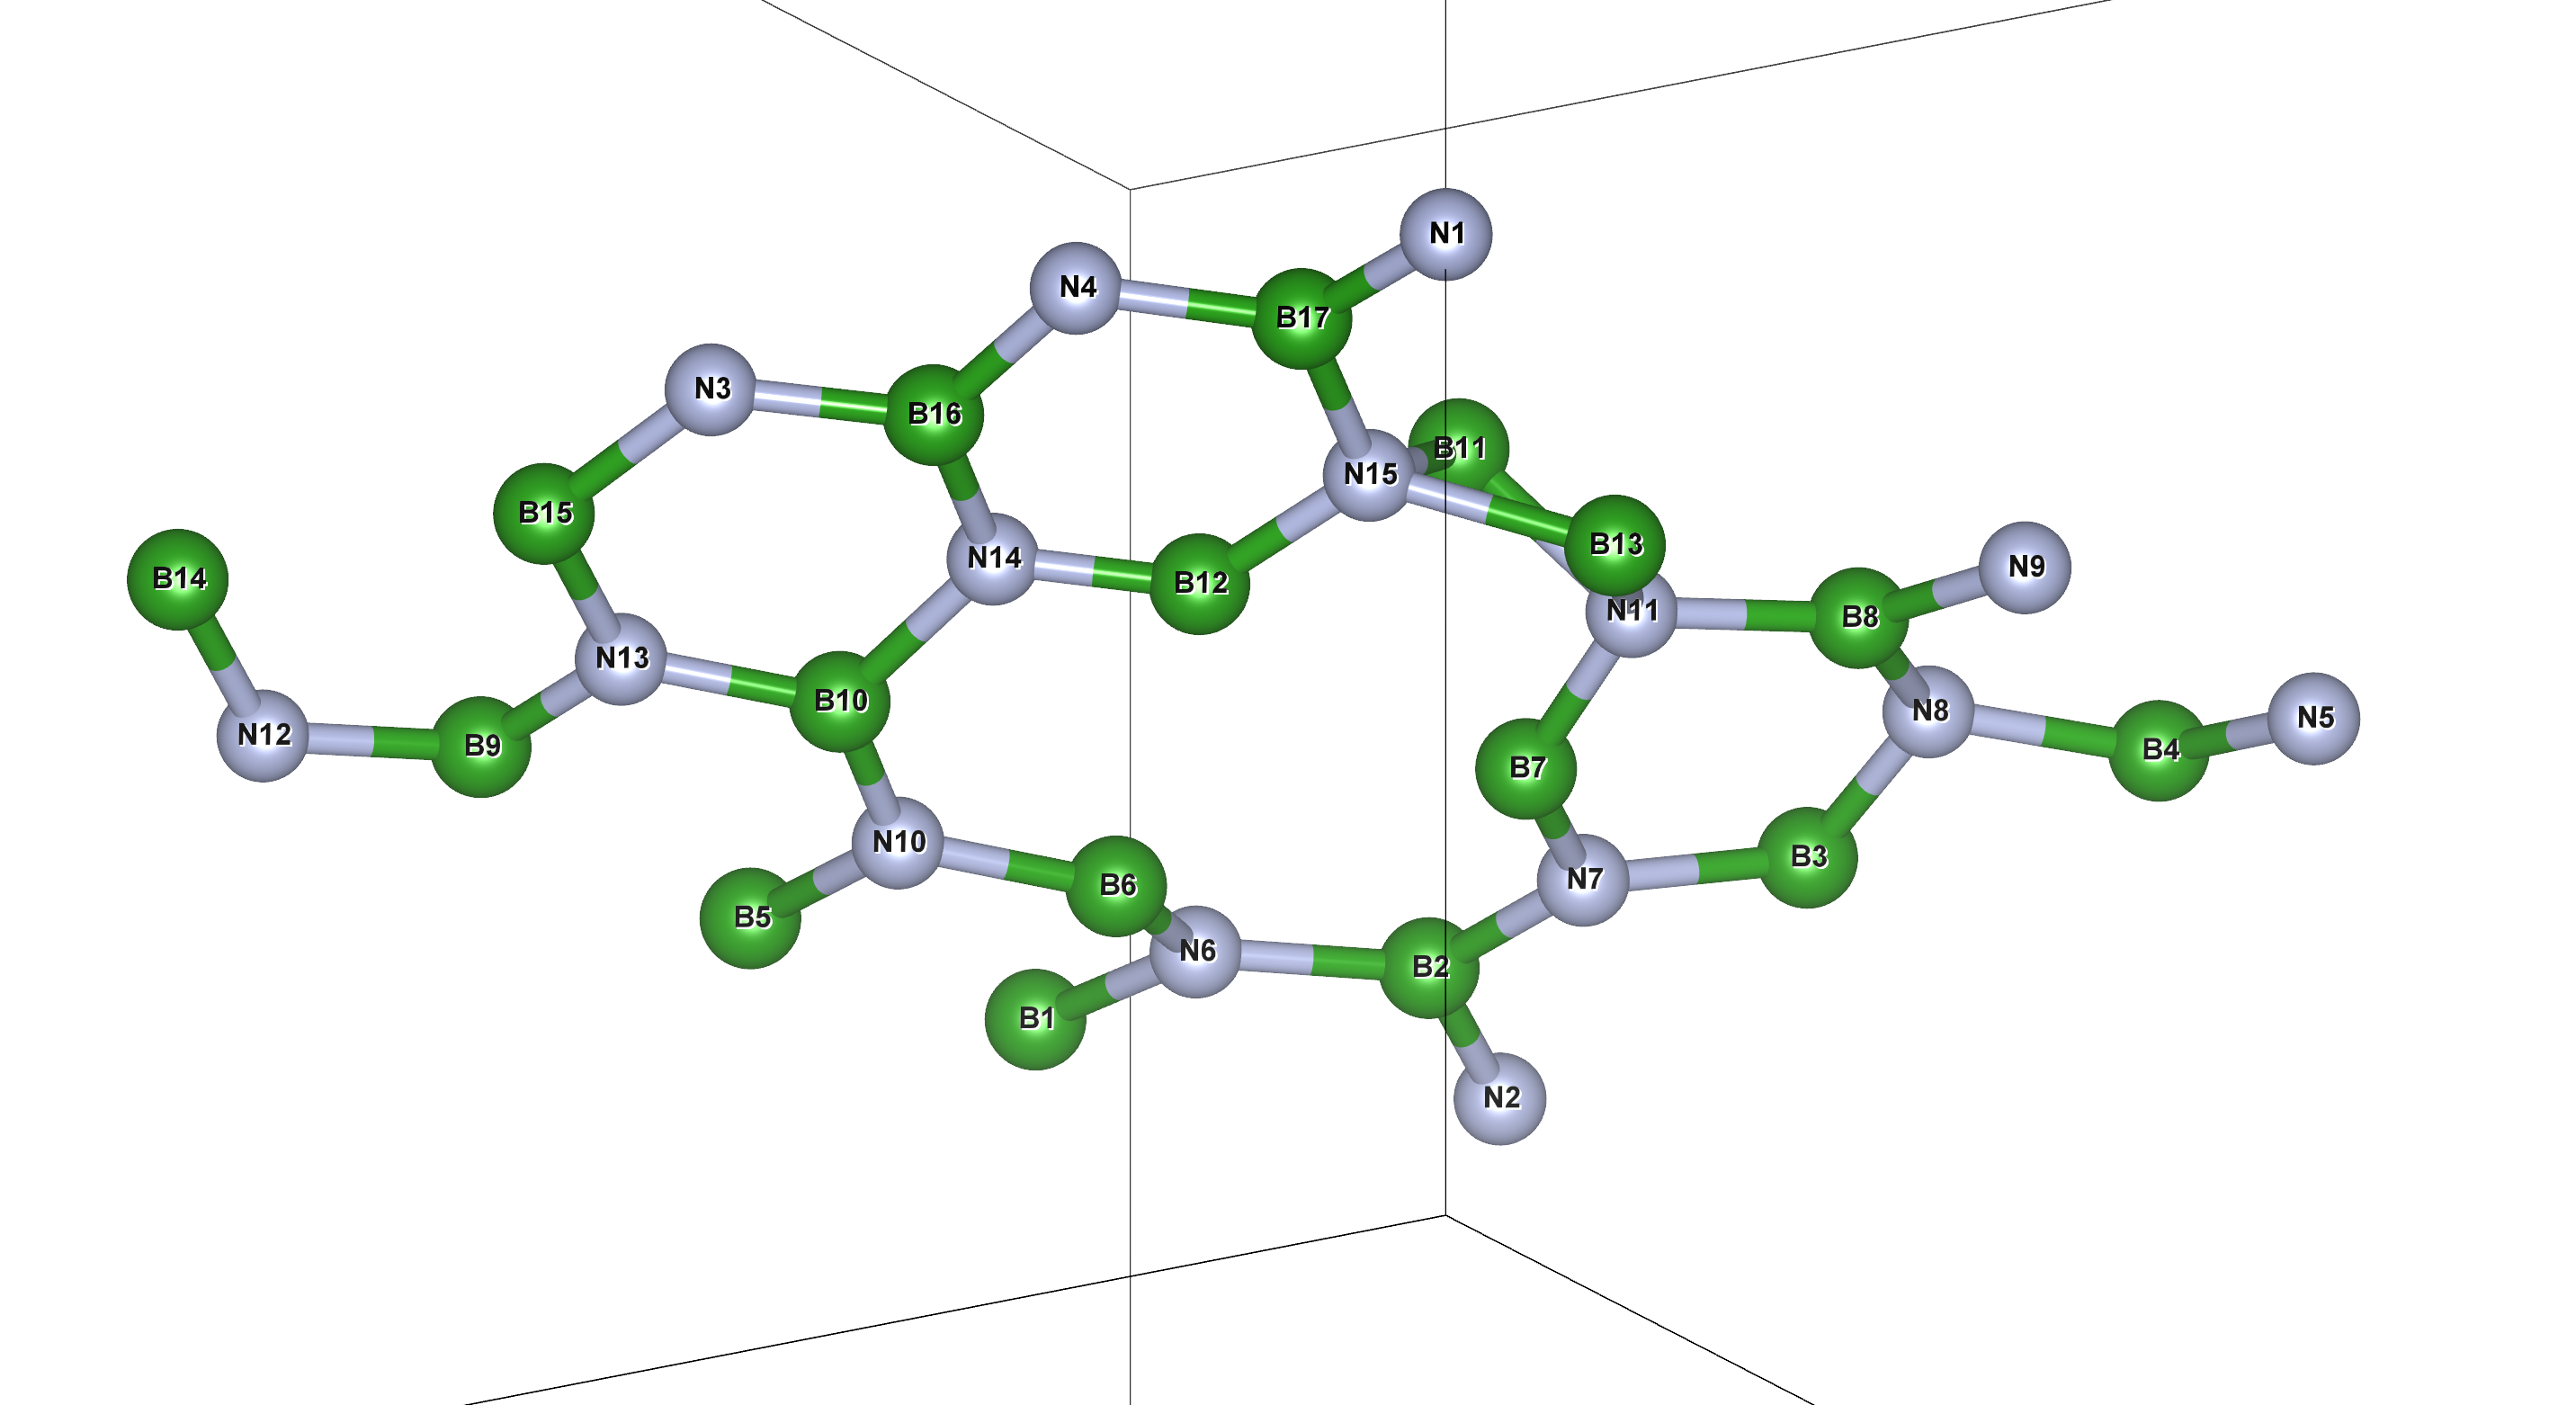
\includegraphics[width=0.49\linewidth]{gambar_hasil/hBN_BB_side_1100K.png}
    \caption{Cacat B\textsubscript{N}, 1100 K}
    \label{subfig:md_bb_1100k}
  \end{subfigure}
  \vspace{1em}
  \begin{subfigure}{\textwidth}
    \centering
    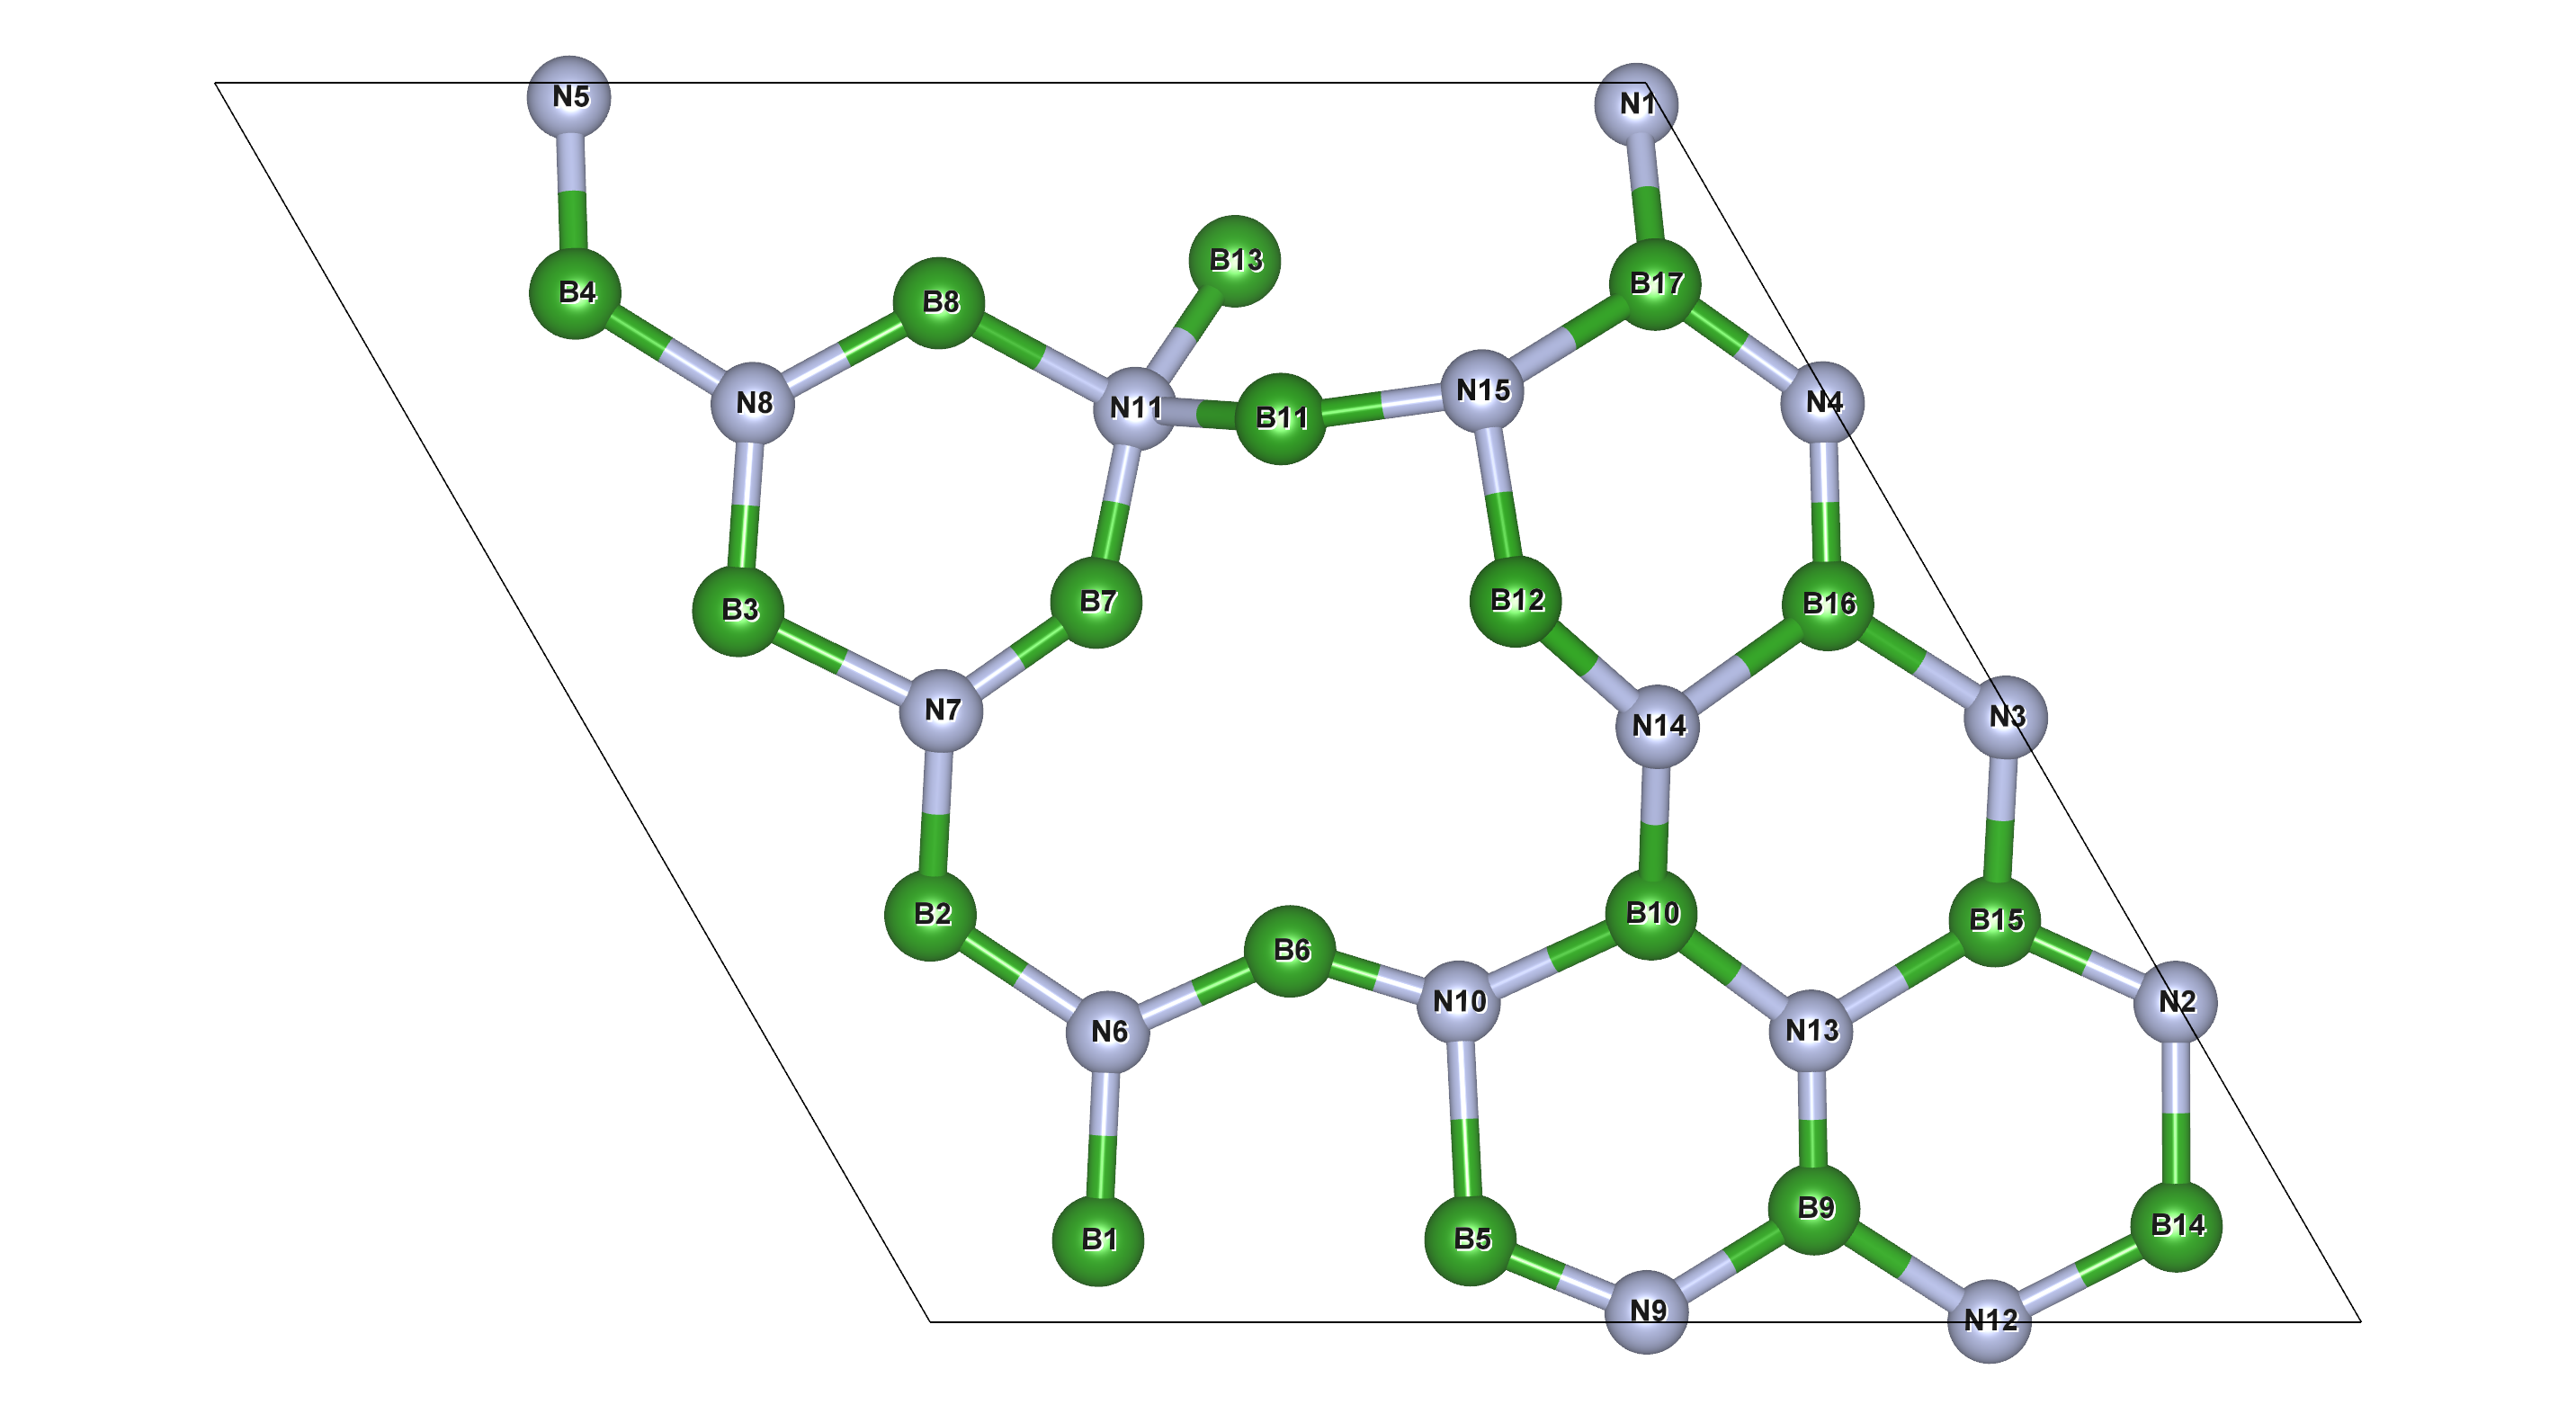
\includegraphics[width=0.49\linewidth]{gambar_hasil/hBN_BB_1225K.png}\hfill
    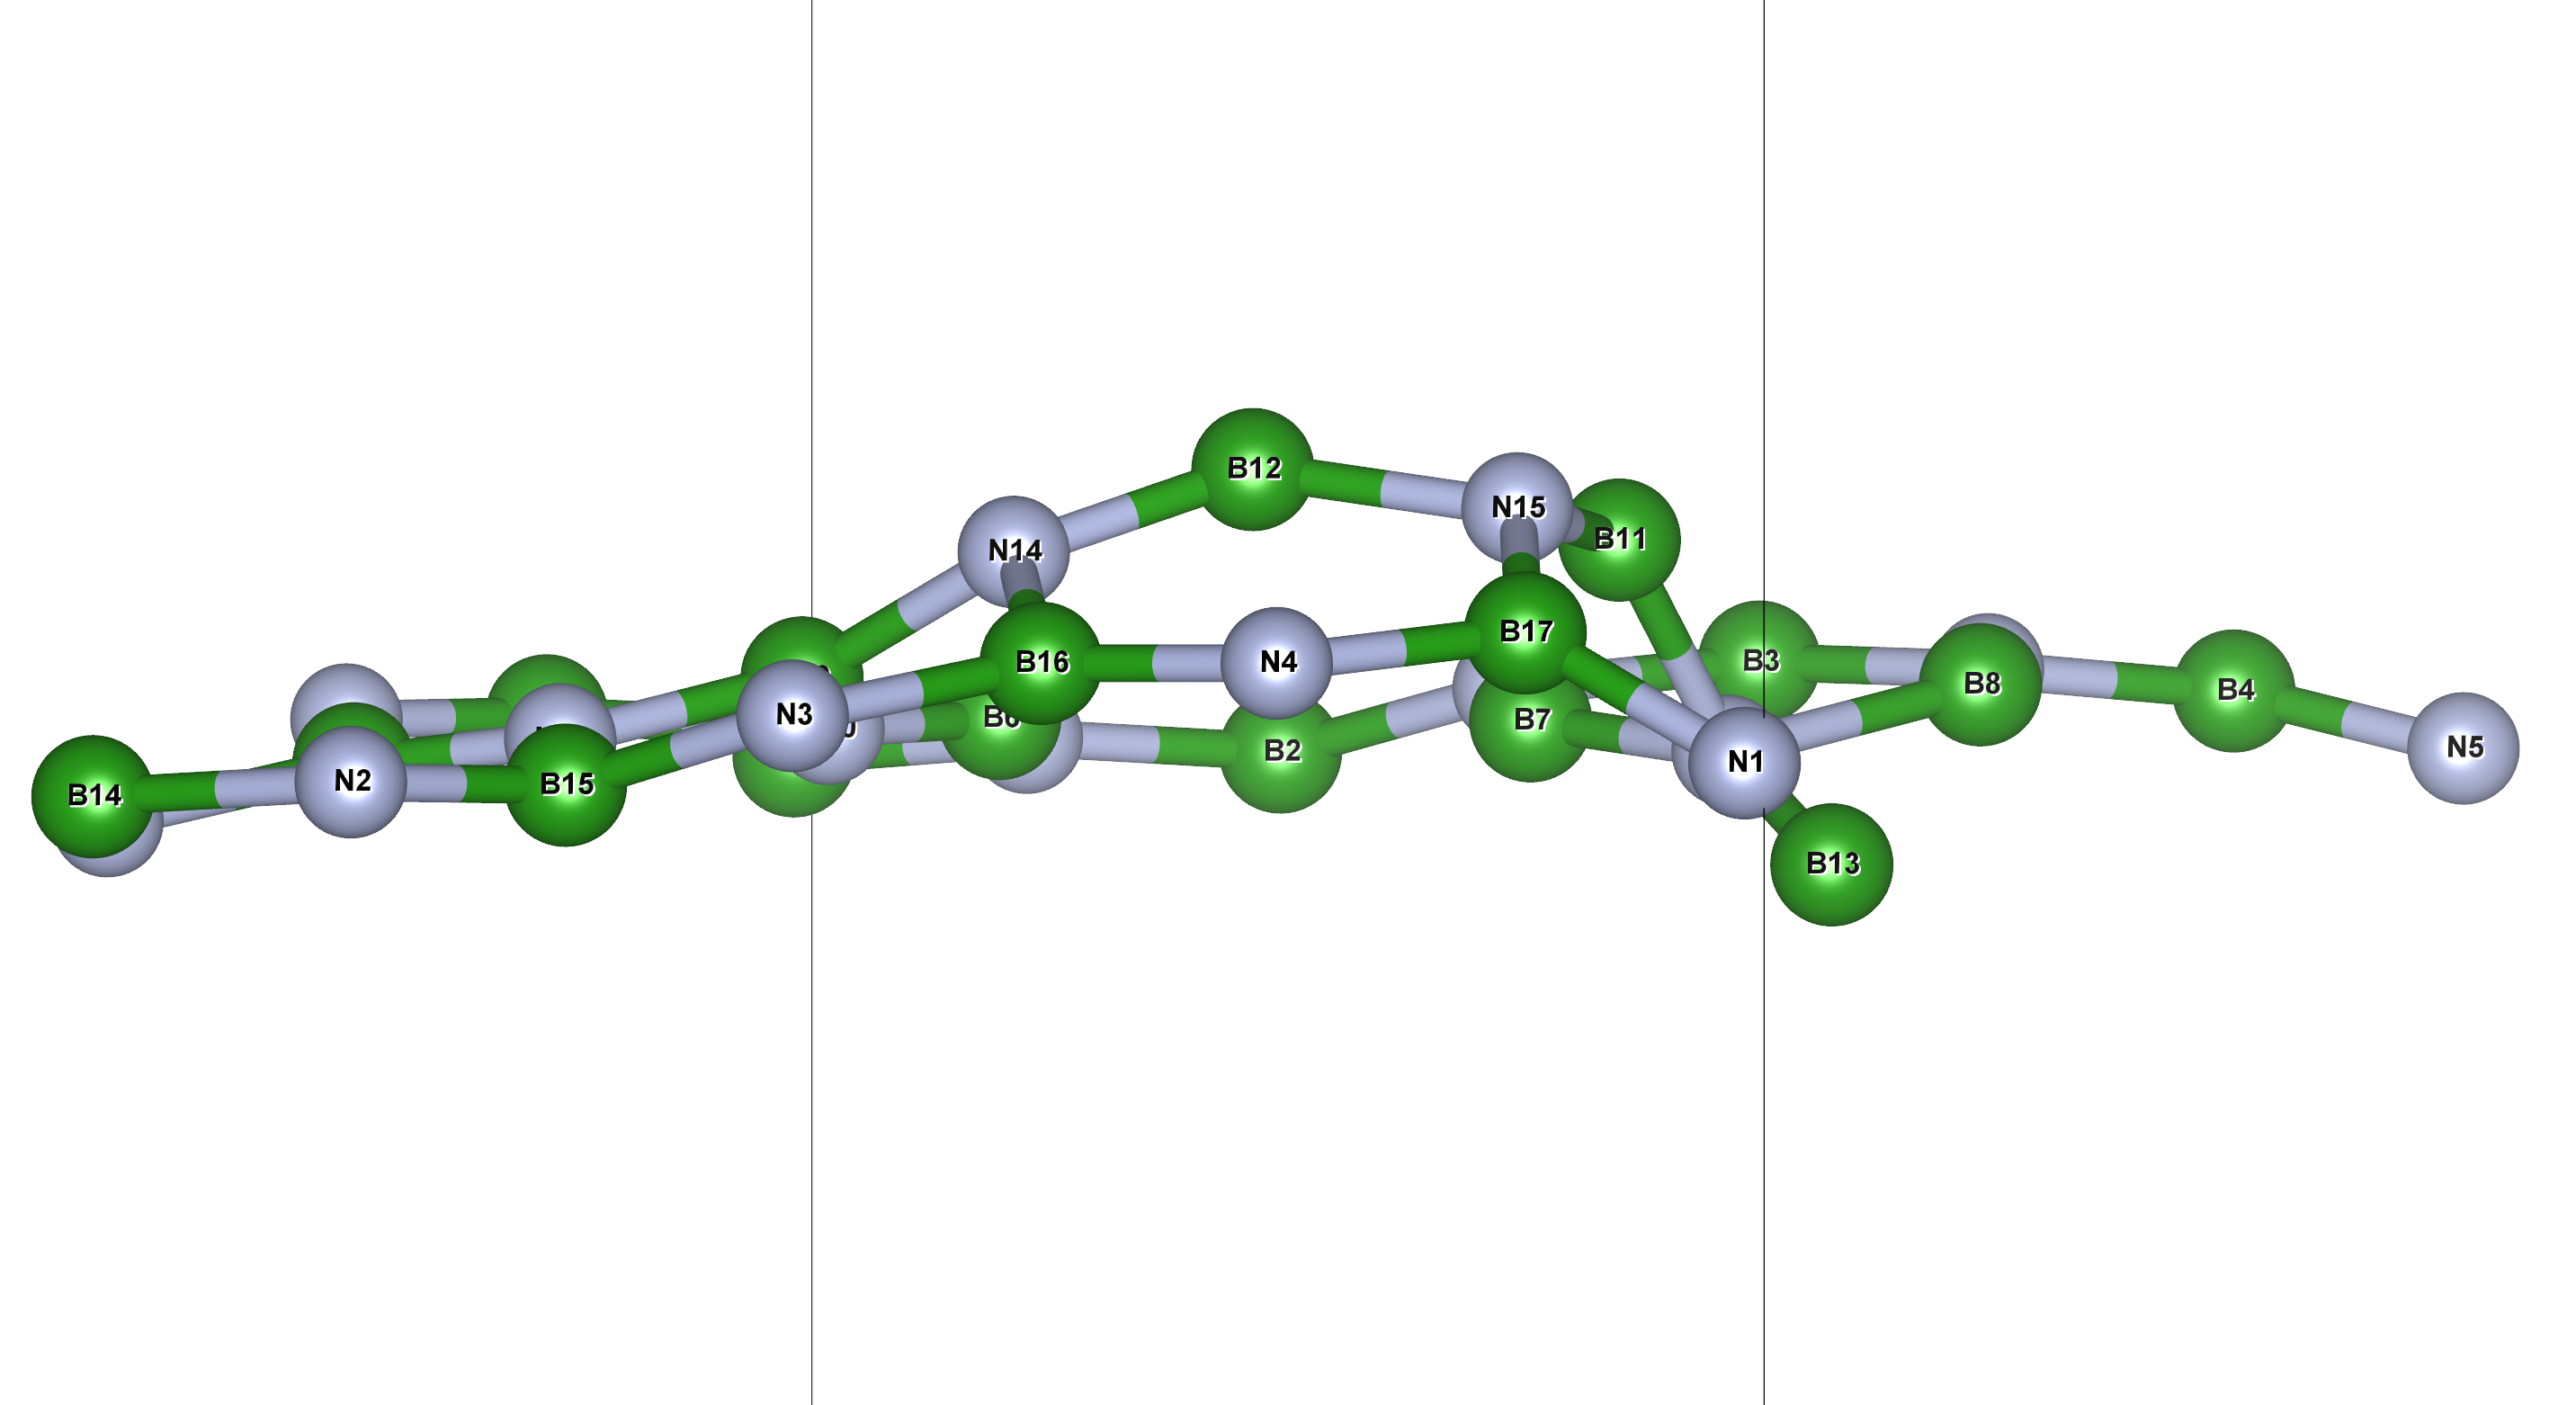
\includegraphics[width=0.49\linewidth]{gambar_hasil/hBN_BB_side_1225K.png}
    \caption{Cacat B\textsubscript{N}, 1225 K}
    \label{subfig:md_bb_1225k}
  \end{subfigure}
    \caption{Visualisasi struktur atomik hasil pemanasan MD. Setiap baris menampilkan tampak atas dan samping untuk sistem dan temperatur yang spesifik.}
  \label{fig:md_structures_per_condition}
\end{figure}

Seperti yang diilustrasikan secara skematis pada Gambar \ref{fig:md_structures_per_condition}, distorsi ini menjadi lebih jelas pada sistem yang mengandung cacat.
Cacat titik bertindak sebagai pusat tegangan (\emph{strain}) lokal, mengganggu keteraturan kisi di sekitarnya dan seringkali memperkuat amplitudo riak termal.
Analisis kuantitatif dari gangguan struktural ini dapat diperoleh melalui fungsi distribusi radial dan pergeseran kuadrat rata-rata.

\subsection{Analisis Tatanan Struktural dan Mobilitas Atomik: RDF dan MSD}
\label{subsec:md_rdf_msd}
Fungsi Distribusi Radial, $g(r)$, memberikan informasi statistik tentang probabilitas menemukan atom pada jarak $r$ dari atom referensi.
Ini adalah alat yang ampuh untuk mengukur tatanan struktural. Pergeseran Kuadrat Rata-rata (MSD) mengukur rata-rata jarak kuadrat yang ditempuh oleh atom dari posisi awalnya seiring waktu.
Ini memberikan wawasan tentang dinamika dan stabilitas struktural material.

%%%%%%%%%%%%%%%%%%%%%%%%%%%%%%%%%%%%%%%%%%%%%%%%%%%%%%%%%%%%%%%%%%%%%%
% PERBAIKAN GAMBAR 2: PLOT RDF DAN MSD (Tata Letak Vertikal, Ukuran Besar)
% Permintaan: Tumpukan vertikal, lebih besar, dan dapat pindah halaman.
% Solusi: Setiap plot ditempatkan dalam 'subfigure' dengan lebar 0.85\textwidth,
% membuatnya sangat jelas dan mudah dibaca. Tumpukan vertikal dari 9 plot ini
% akan menghasilkan 'figure' yang sangat tinggi, yang akan ditangani oleh
% mekanisme float LaTeX ([htbp!]) dengan memindahkannya ke halaman float [p].
%%%%%%%%%%%%%%%%%%%%%%%%%%%%%%%%%%%%%%%%%%%%%%%%%%%%%%%%%%%%%%%%%%%%%%
\begin{figure}[htbp]
  \centering

  % --- Gambar gabungan untuk Murni ---
  \begin{subfigure}{0.9\textwidth}
    \centering
    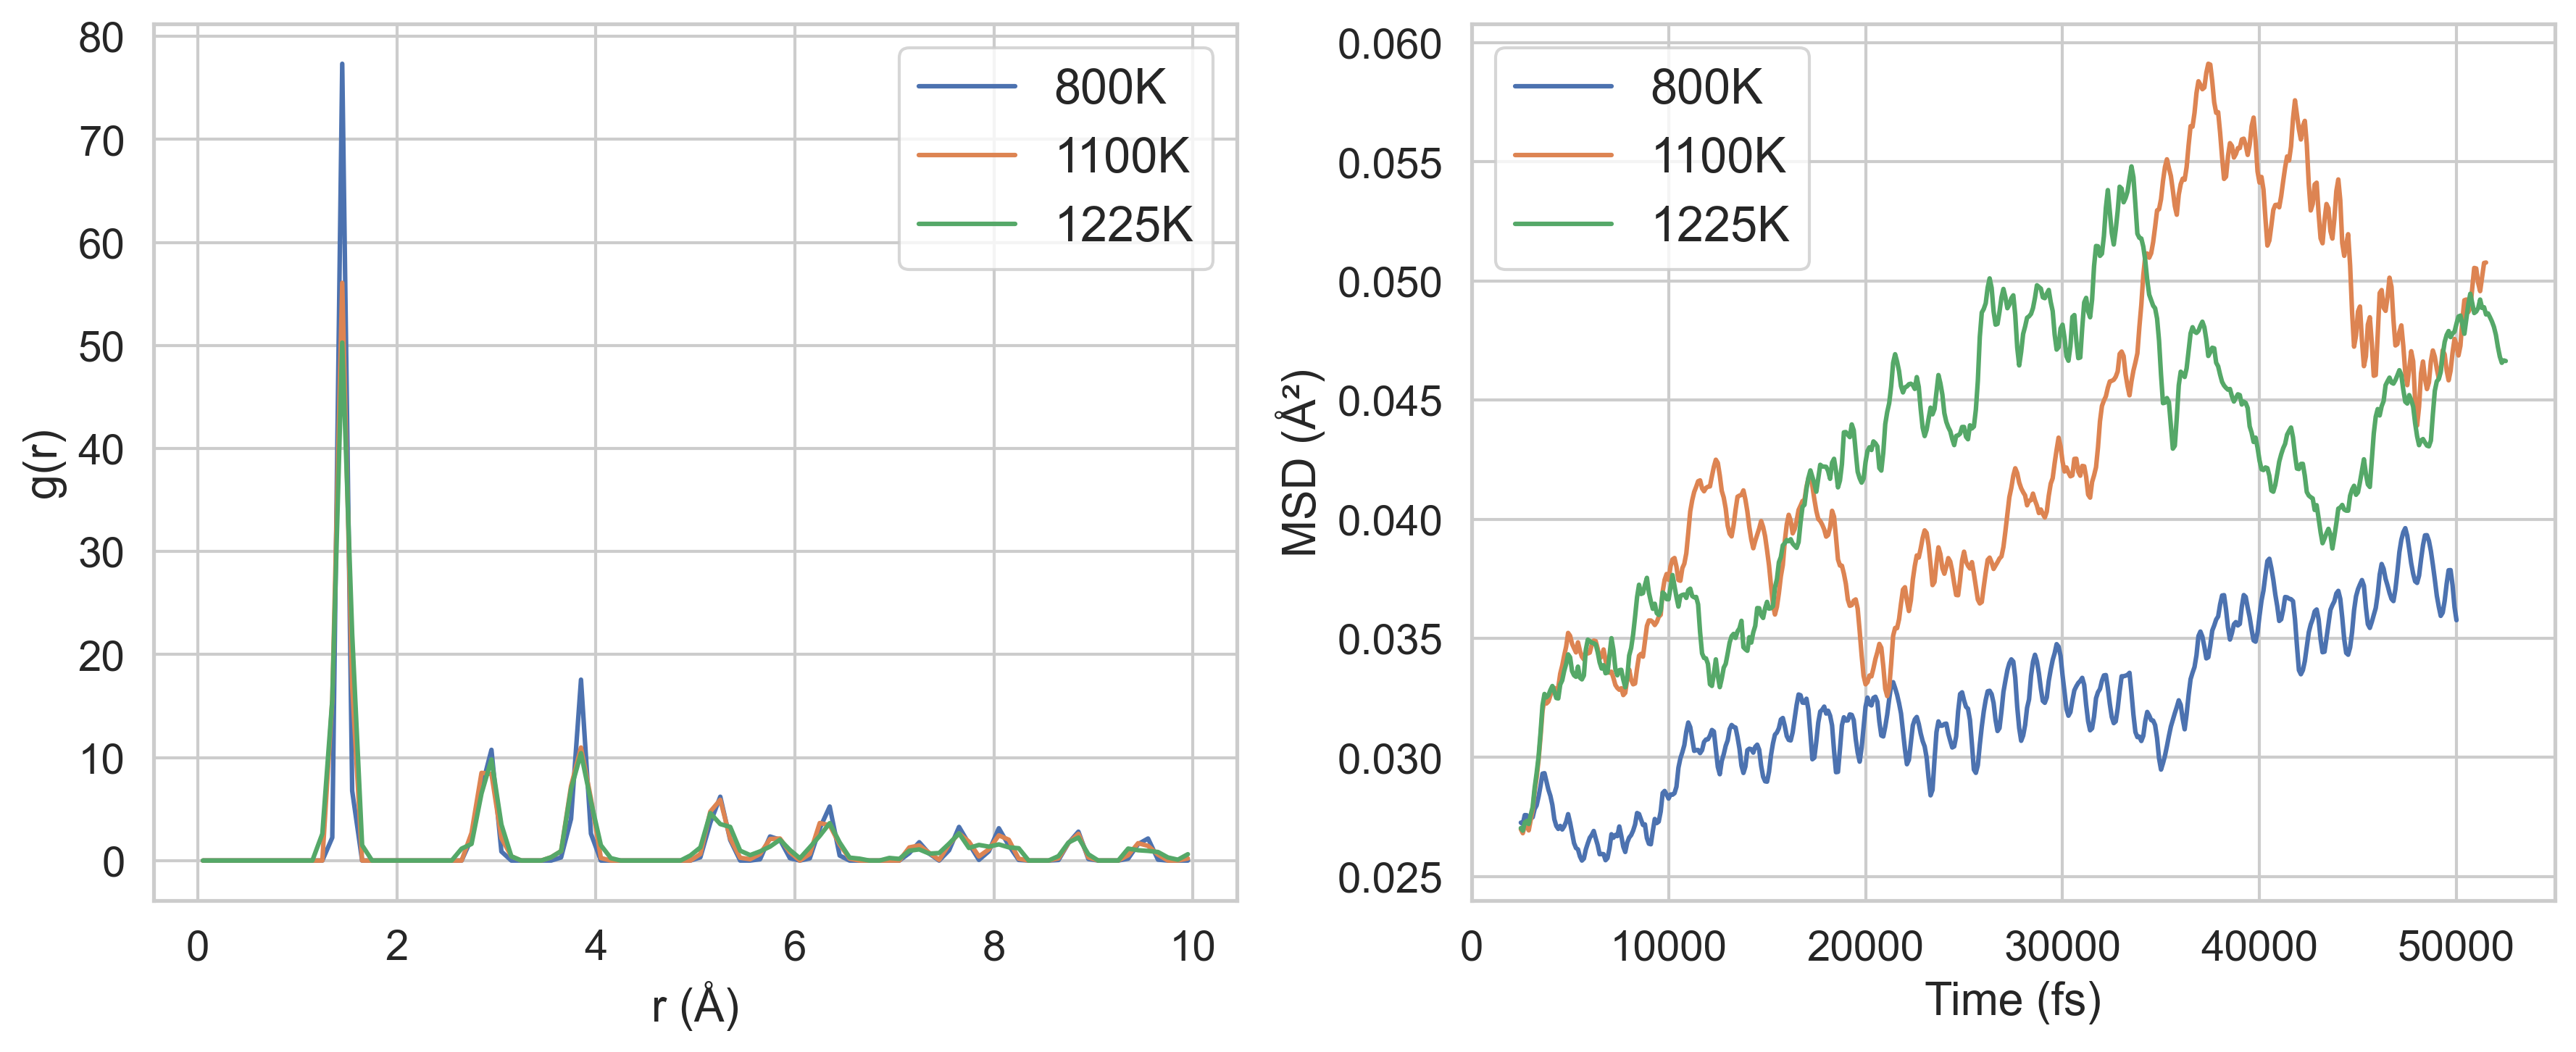
\includegraphics[width=\linewidth]{pure_combined_notitle.png}
    \caption{hBN murni pada suhu 800 K, 1100 K, dan 1225 K}
    \label{subfig:rdf_msd_pure_combined}
  \end{subfigure}

  \vspace{1em}

  % --- Gambar gabungan untuk cacat N_B ---
  \begin{subfigure}{0.9\textwidth}
    \centering
    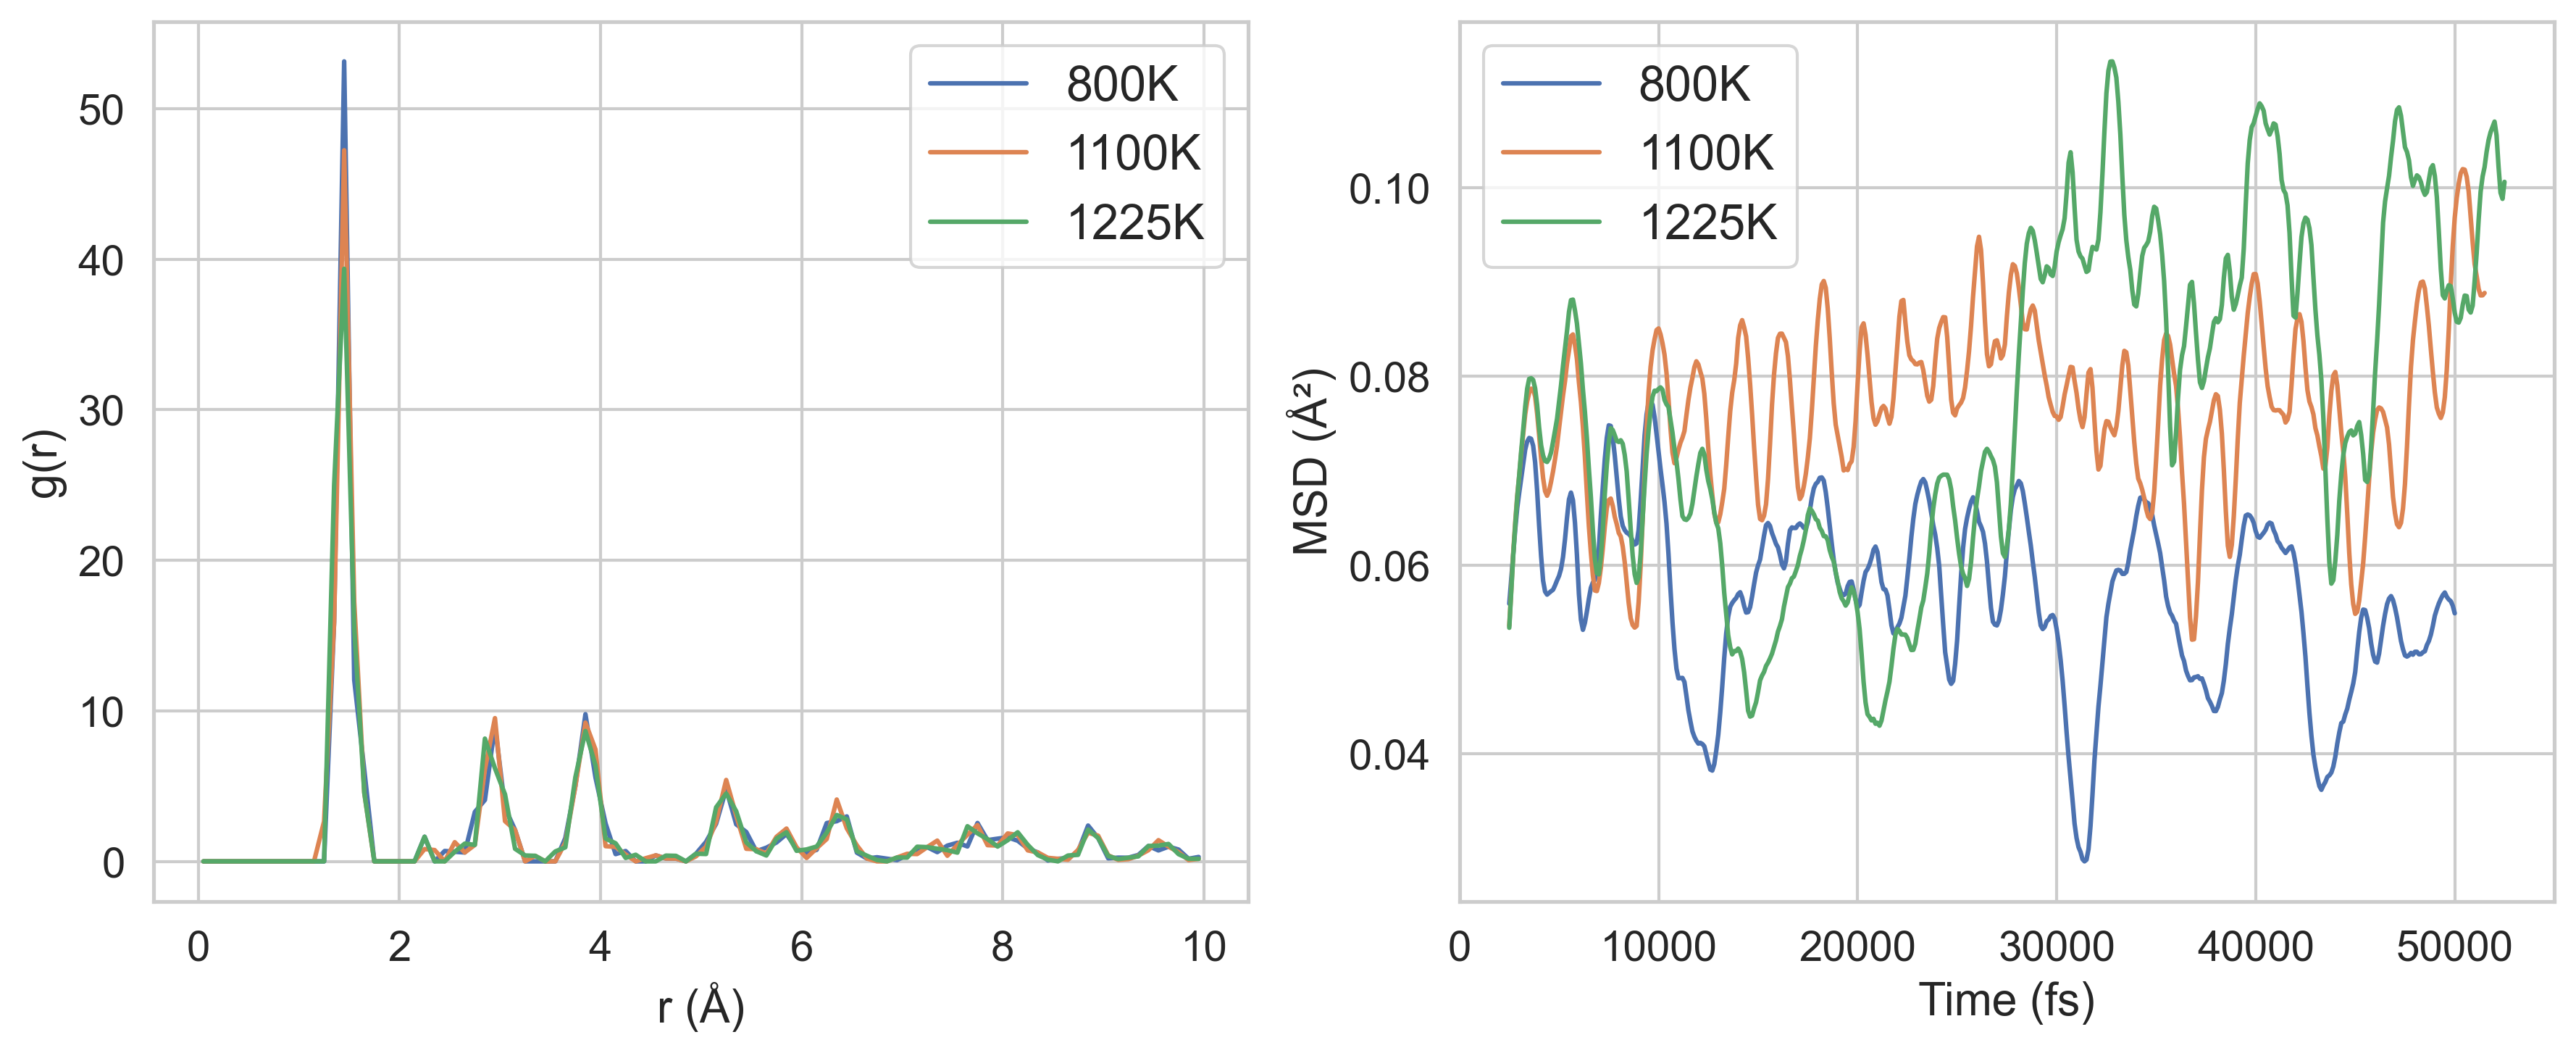
\includegraphics[width=\linewidth]{NN_combined_notitle.png}
    \caption{Cacat N\textsubscript{B} pada suhu 800 K, 1100 K, dan 1225 K}
    \label{subfig:rdf_msd_nn_combined}
  \end{subfigure}

  \vspace{1em}

  % --- Gambar gabungan untuk cacat B_N ---
  \begin{subfigure}{0.9\textwidth}
    \centering
    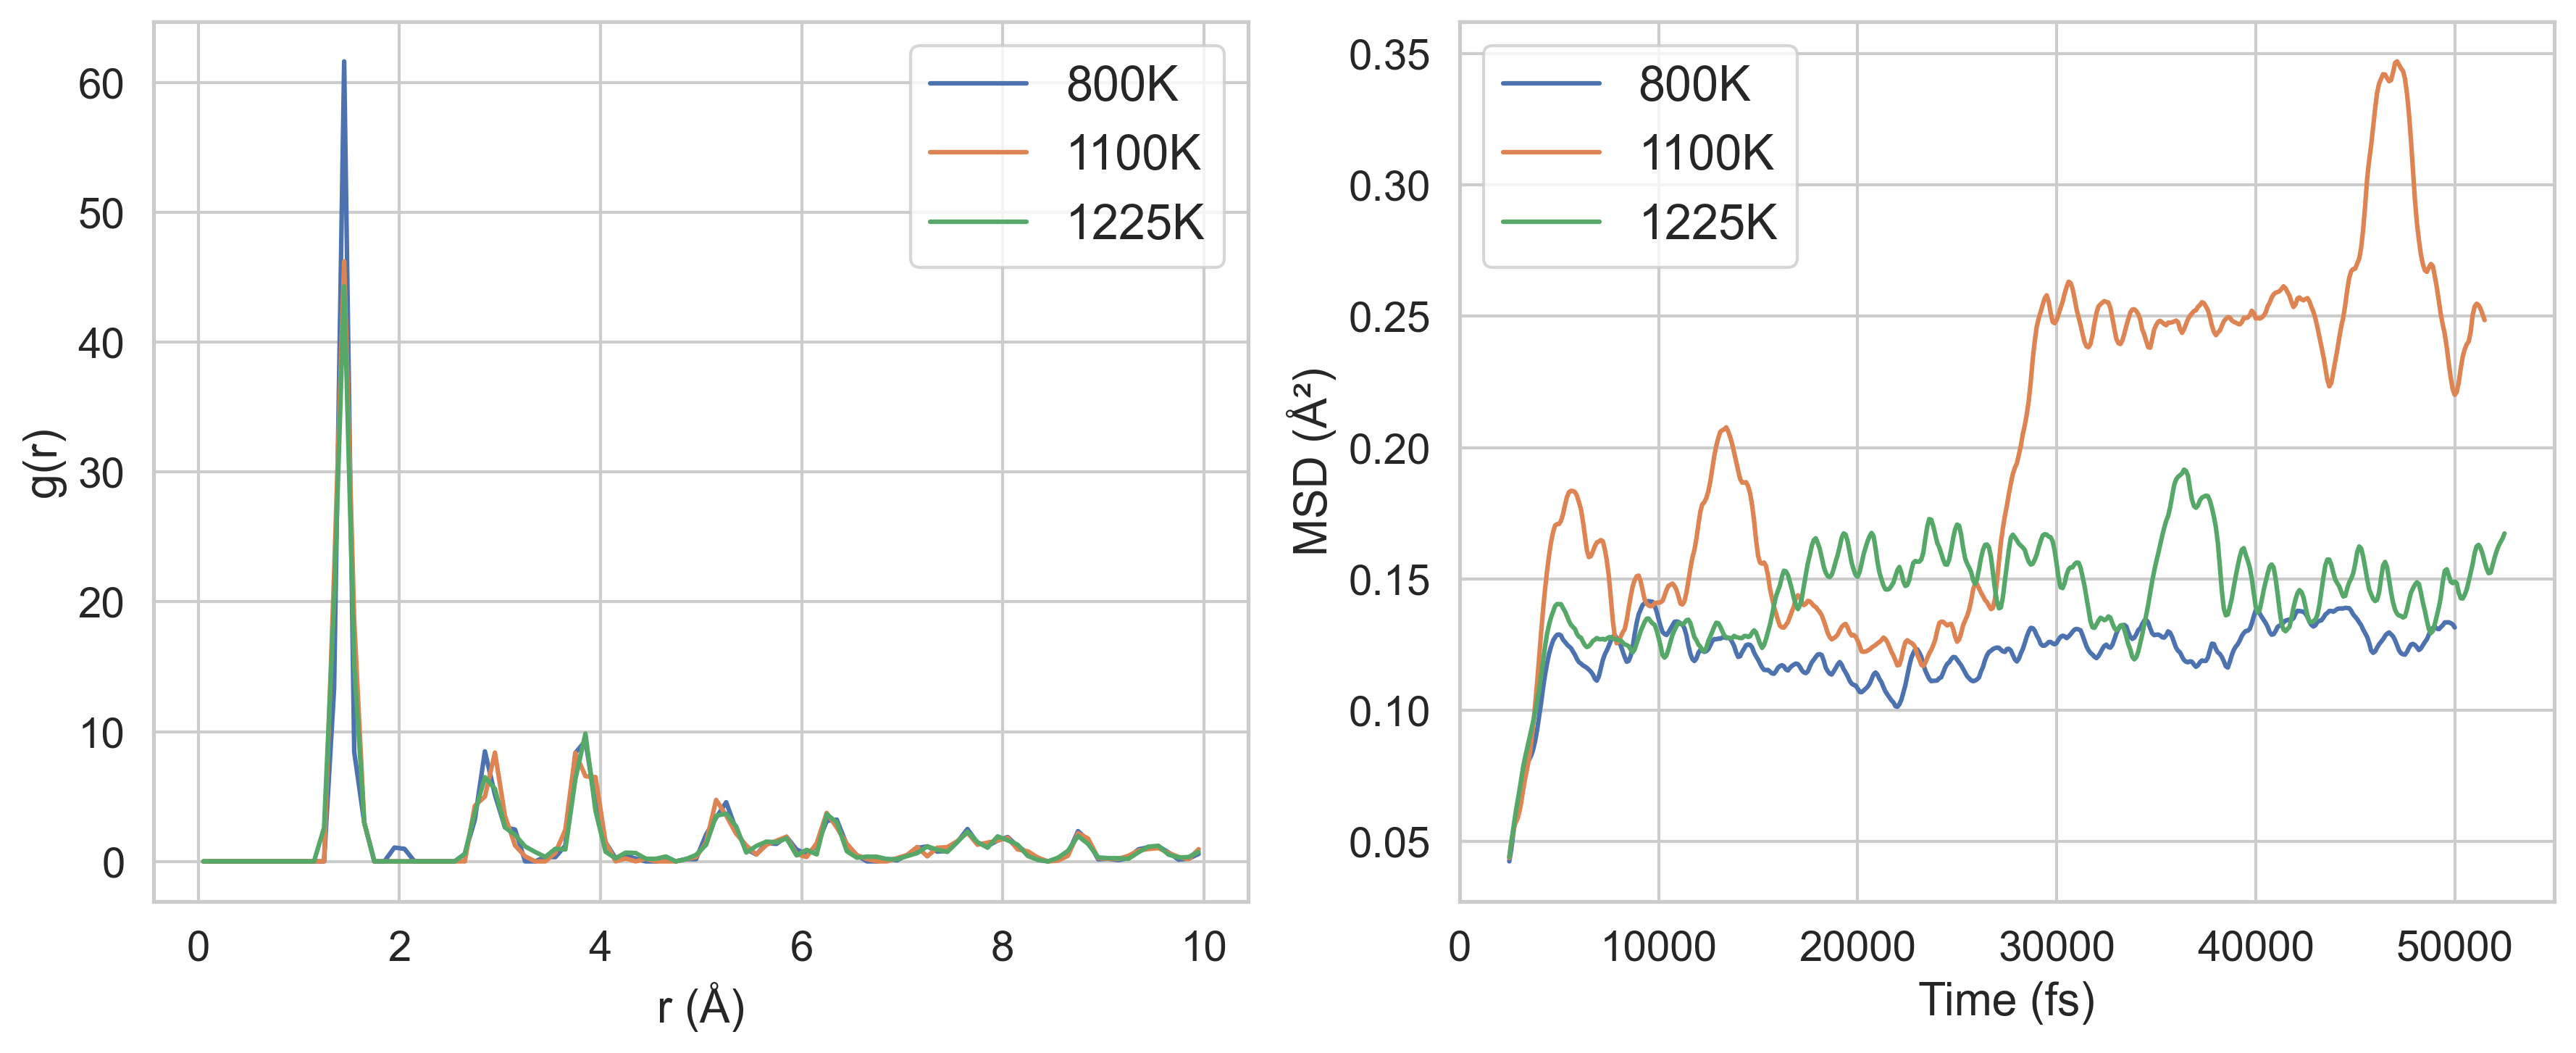
\includegraphics[width=\linewidth]{BB_combined_notitle.png}
    \caption{Cacat B\textsubscript{N} pada suhu 800 K, 1100 K, dan 1225 K}
    \label{subfig:rdf_msd_bb_combined}
  \end{subfigure}

  \caption{Plot RDF dan MSD gabungan untuk variasi struktur hBN: murni, cacat N\textsubscript{B}, dan cacat B\textsubscript{N}, masing-masing pada suhu 800 K, 1100 K, dan 1225 K.}
  \label{fig:rdf_msd_gabungan}
\end{figure}

Gambar \ref{fig:rdf_msd_gabungan} menunjukkan plot RDF dan MSD untuk setiap sistem dan temperatur.
Beberapa tren kunci dapat diidentifikasi dari plot RDF:
\begin{itemize}
    \item Pengaruh Temperatur: Untuk semua sistem, seiring dengan meningkatnya temperatur dari 800 K ke 1225 K, puncak-puncak RDF menjadi lebih rendah dan lebih lebar.
Ini adalah indikasi klasik dari peningkatan gangguan termal (\emph{thermal disorder}).
Amplitudo vibrasi atom yang lebih besar menyebabkan distribusi jarak antar-atom yang lebih luas, sehingga mengurangi korelasi posisi jarak jauh dan "melelehkan" puncak-puncak yang tajam.
\item Pengaruh Cacat: Pada temperatur yang sama, sistem dengan cacat (N\textsubscript{B} dan B\textsubscript{N}) umumnya menunjukkan puncak yang sedikit lebih lebar dibandingkan sistem murni.
Ini mengindikasikan bahwa cacat mengintroduksi gangguan struktural statis di atas gangguan termal dinamis.
Kehadiran ikatan yang "salah" (misalnya, B-B atau N-N di sekitar cacat antisite) dan relaksasi kisi lokal di sekitarnya memutus periodisitas sempurna dan mengurangi tatanan kristal.
Sistem B\textsubscript{N} menunjukkan pelebaran puncak yang paling signifikan, menandakan distorsi lokal terbesar, yang merupakan prasyarat penting untuk fenomena elektronik yang akan dibahas nanti.
\end{itemize}

Dari plot MSD pada Gambar \ref{fig:rdf_msd_gabungan}, perilaku dinamis sistem dapat dianalisis:
\begin{itemize}
    \item Stabilitas Fasa Padat: Untuk semua kasus, MSD meningkat seiring waktu tetapi tidak menunjukkan rezim difusif linier yang jelas (seperti pada cairan), melainkan menunjukkan perilaku sub-difusif yang khas untuk atom dalam fasa padat pada temperatur tinggi.
Ini mengonfirmasi bahwa monolayer hBN, bahkan pada 1225 K, tetap dalam keadaan padat dan tidak meleleh selama simulasi.
\item Mobilitas Termal: Kemiringan kurva MSD secara kualitatif terkait dengan mobilitas atom.
Semakin curam kemiringannya, semakin tinggi mobilitas atom dan semakin rendah stabilitas strukturalnya.
Terlihat jelas bahwa untuk setiap jenis sistem, MSD meningkat lebih cepat pada temperatur yang lebih tinggi, yang konsisten dengan eksitasi termal yang lebih besar.
\item Dampak Cacat pada Stabilitas: Perbandingan antar sistem pada temperatur tertinggi (1225 K) sangat informatif.
Sistem murni menunjukkan MSD terendah, menandakan stabilitas struktural tertinggi. Sistem N\textsubscript{B} menunjukkan mobilitas yang lebih tinggi.
Secara signifikan, sistem B\textsubscript{N} menunjukkan MSD tertinggi dengan selisih yang jelas.
Ini menyiratkan bahwa atom-atom dalam sistem dengan cacat B\textsubscript{N} adalah yang paling mobile dan strukturnya paling tidak stabil secara dinamis.
Mobilitas atomik yang tinggi ini adalah manifestasi makroskopis dari vibrasi kisi (fonon) beramplitudo besar.
Lingkungan yang sangat dinamis dan terdistorsi di sekitar cacat B\textsubscript{N} inilah yang menciptakan kondisi untuk kopling spin-fonon yang kuat, seperti yang akan dibahas pada Bagian \ref{subsec:hbn_defek_bn}.
\end{itemize}

\section{Pengaruh Temperatur pada Sifat Elektronik Monolayer hBN Murni}
\label{sec:hbn_murni}
Analisis terhadap sistem hBN murni berfungsi sebagai dasar untuk memahami bagaimana sifat elektronik intrinsik material merespons eksitasi termal, sebelum mempertimbangkan efek yang lebih kompleks dari cacat.
\subsection{Karakteristik Elektronik Dasar hBN Murni (Sistem Referensi)}
\label{subsec:hbn_murni_dasar}
Sebagai titik acuan, sifat elektronik monolayer hBN murni dalam kondisi \emph{pristine} (struktur ideal teroptimasi, mendekati 0 K) dianalisis terlebih dahulu.
Hasil kalkulasi DFT (Gambar \ref{fig:hbn_pristine_bs_pdos}) menunjukkan bahwa hBN murni adalah isolator celah pita lebar non-magnetik.
Struktur pita menunjukkan celah pita langsung (\emph{direct band gap}) sebesar $E_g = 4.446$ eV pada titik K di Zona Brillouin.
Analisis Kerapatan Keadaan Terproyeksi (PDOS) mengonfirmasi bahwa puncak pita valensi (VBM) didominasi oleh orbital N $2p_z$ (membentuk pita $\pi$), sedangkan dasar pita konduksi (CBM) didominasi oleh orbital B $2p_z$ (membentuk pita $\pi^*$), sesuai dengan literatur \citep{Sachs2011}.
Visualisasi kerapatan muatan (tidak ditampilkan) menunjukkan akumulasi elektron di sekitar atom nitrogen yang lebih elektronegatif, mengindikasikan ikatan B-N yang bersifat kovalen polar.
\begin{figure}[htbp!] % PERUBAHAN: Ukuran gambar diperbesar
    \centering
    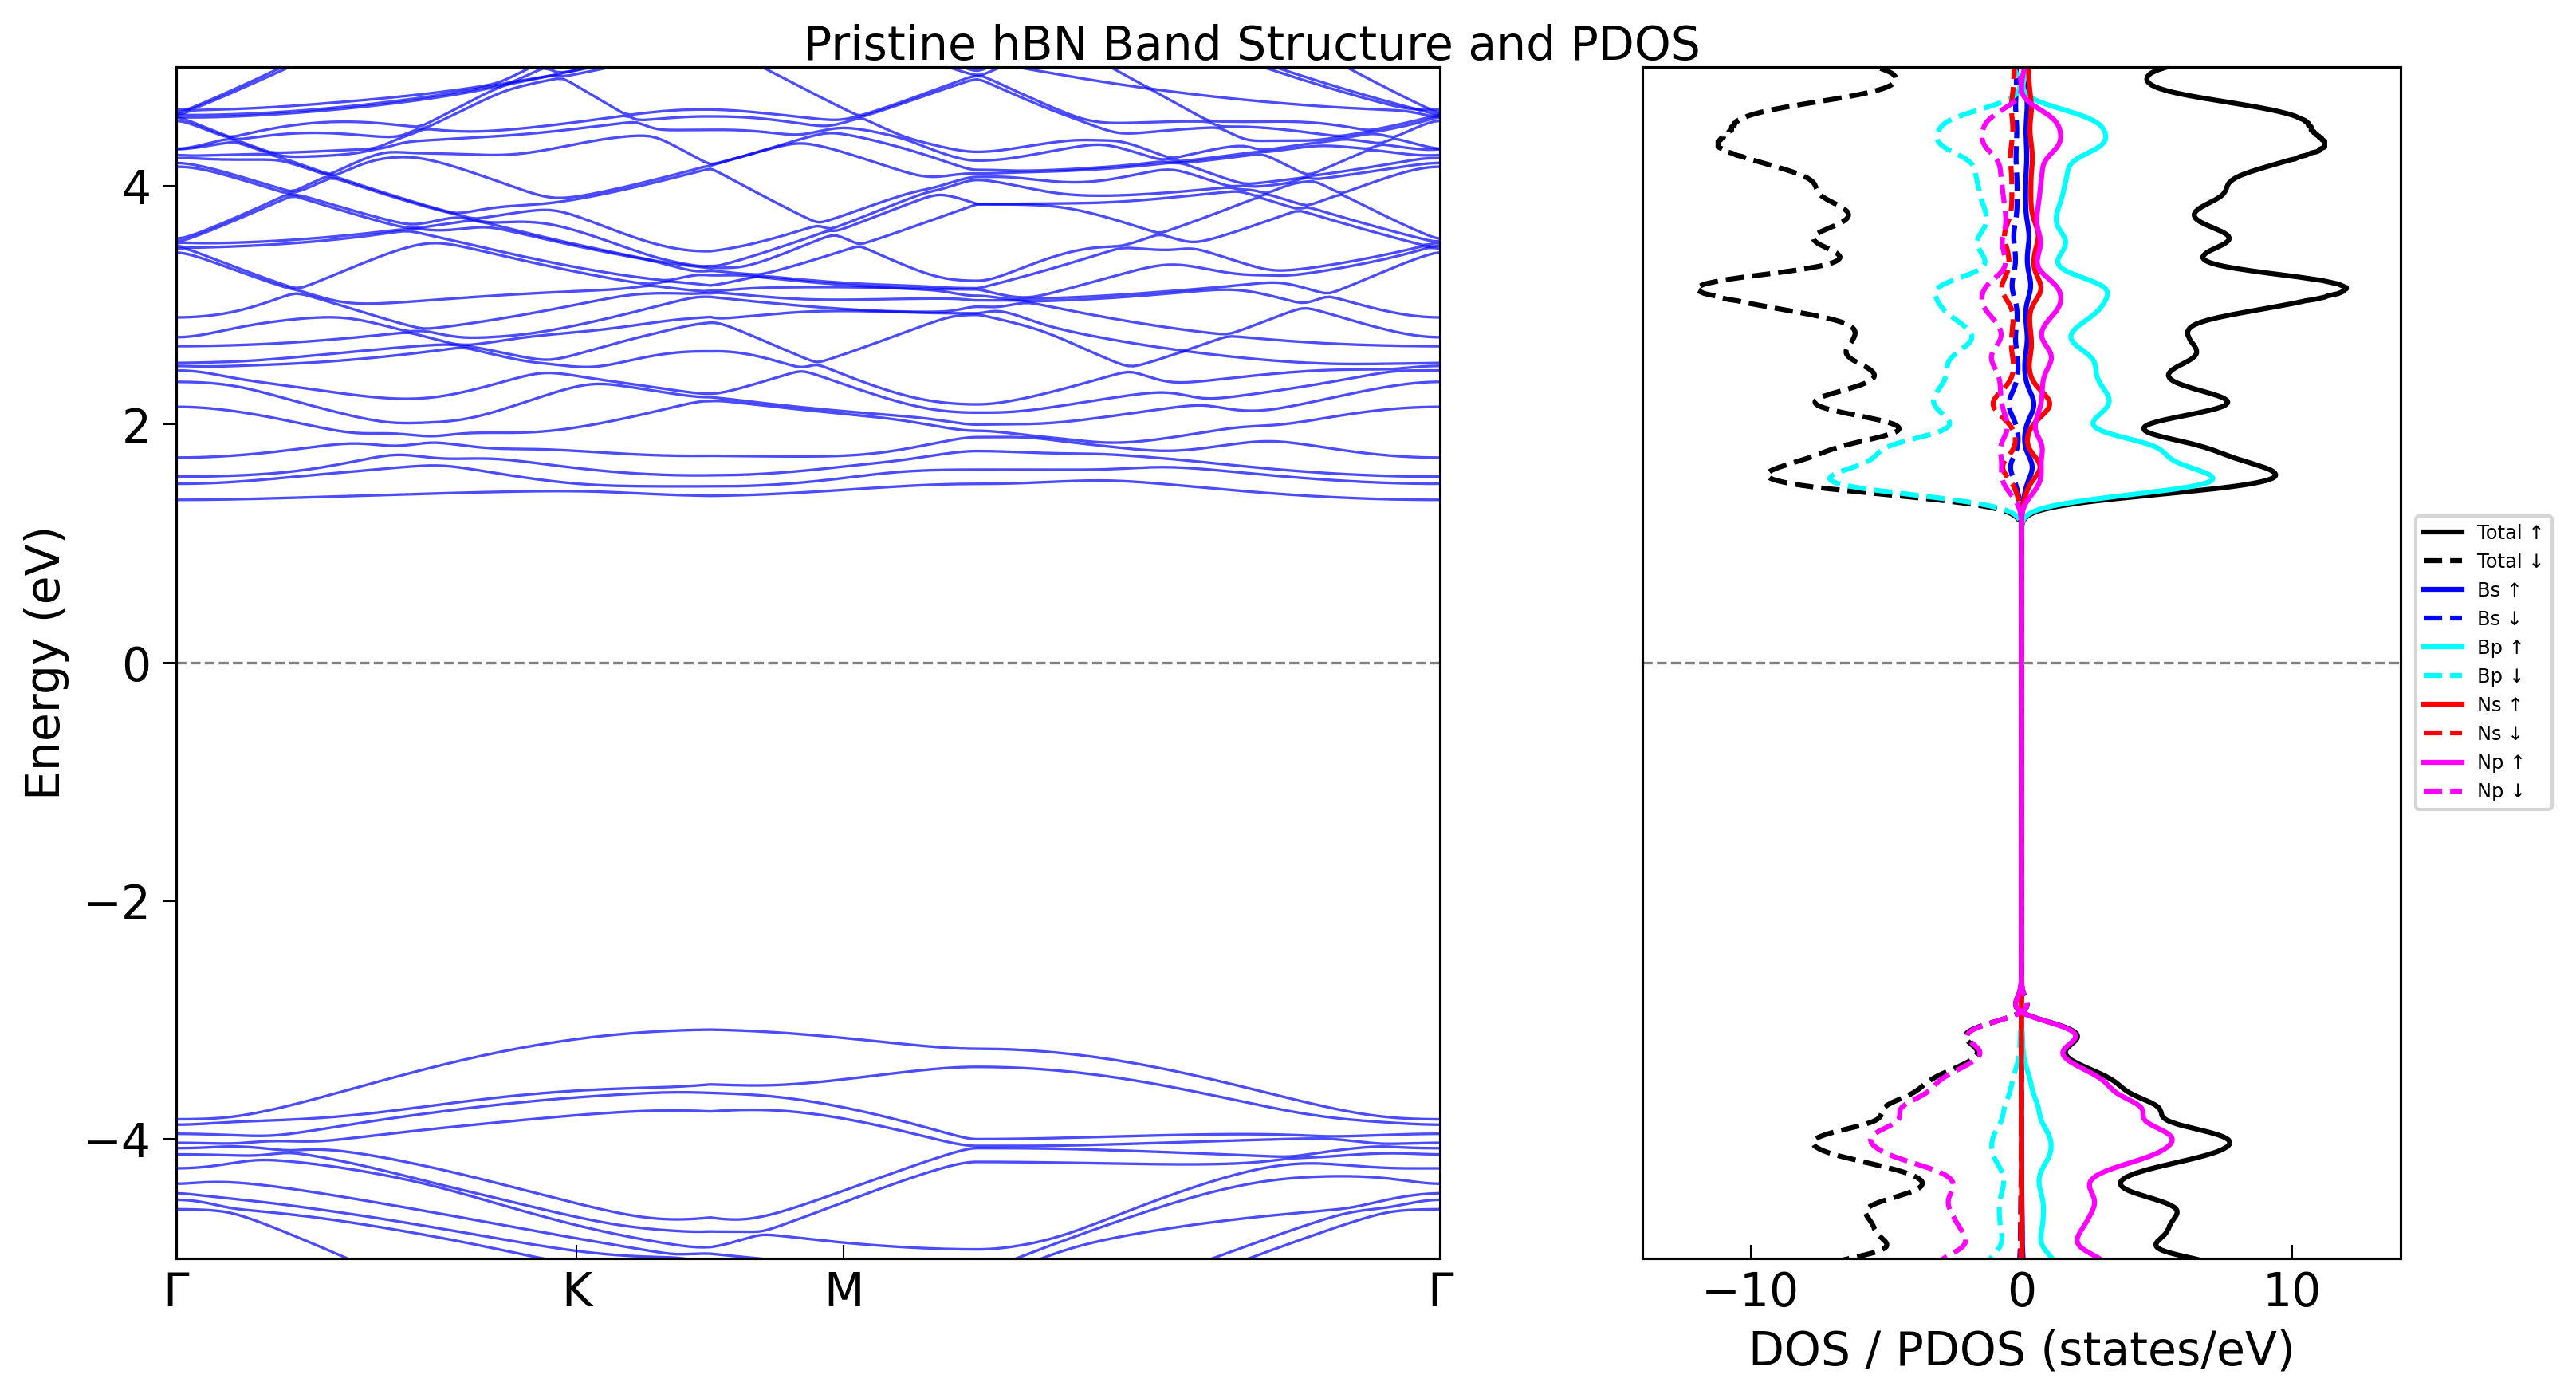
\includegraphics[width=0.95\textwidth]{gambar_hasil/simple_bands_pdos_pristine.png}
    \caption{Struktur pita elektronik dan Kerapatan Keadaan Terproyeksi (PDOS) untuk monolayer hBN murni (\emph{pristine}).
Energi Fermi ($E_F = -0.445$ eV) diset sebagai referensi energi nol pada plot PDOS.}
    \label{fig:hbn_pristine_bs_pdos}
\end{figure}

\subsection{Renormalisasi Celah Pita oleh Kopling Elektron-Fonon (EPC)}
\label{subsec:hbn_murni_termal}
Ketika temperatur dinaikkan, struktur atomik yang diperoleh dari MD digunakan untuk kalkulasi DFT.
Hasilnya (dirangkum dalam Tabel \ref{tab:hbn_murni_suhu} dan diilustrasikan pada Gambar \ref{fig:hbn_pure_800K} hingga \ref{fig:hbn_pure_1225K}) menunjukkan tren penurunan monoton dari celah pita energi, dari $4.446$ eV pada kondisi \emph{pristine} menjadi $4.069$ eV pada 1225 K. Penurunan ini dikenal sebagai pergeseran merah (\emph{redshift}) termal.
\begin{table}[htbp!] % STANDARISASI: Menggunakan [htbp!]
  \centering
  \caption{Sifat Elektronik Monolayer hBN Murni sebagai Fungsi Temperatur.}
  \label{tab:hbn_murni_suhu}
  \begin{tabular}{lccccc}
    \toprule
    Temperatur (K) & VBM (eV) & CBM (eV) & $E_g$ (eV) & $\Delta E_g$ dari Pristine (eV) & $E_F$ (eV) \\
    \midrule
    Pristine (Ref.) & -3.081 &  1.365 & 4.446 &  0.000 & -0.445 \\
    800             & -3.238 &  1.177 & 4.415 & -0.031 & -0.304 \\
    1100            & -3.183 &  1.145 & 4.328 & -0.118 & -0.323 \\
    1225            & -3.112 &  0.957 & 4.069 & -0.377 & -0.430 \\
    \bottomrule
  \end{tabular}
\end{table}

\begin{figure}[htbp!] % PERUBAHAN: Ukuran gambar diperbesar
    \centering
    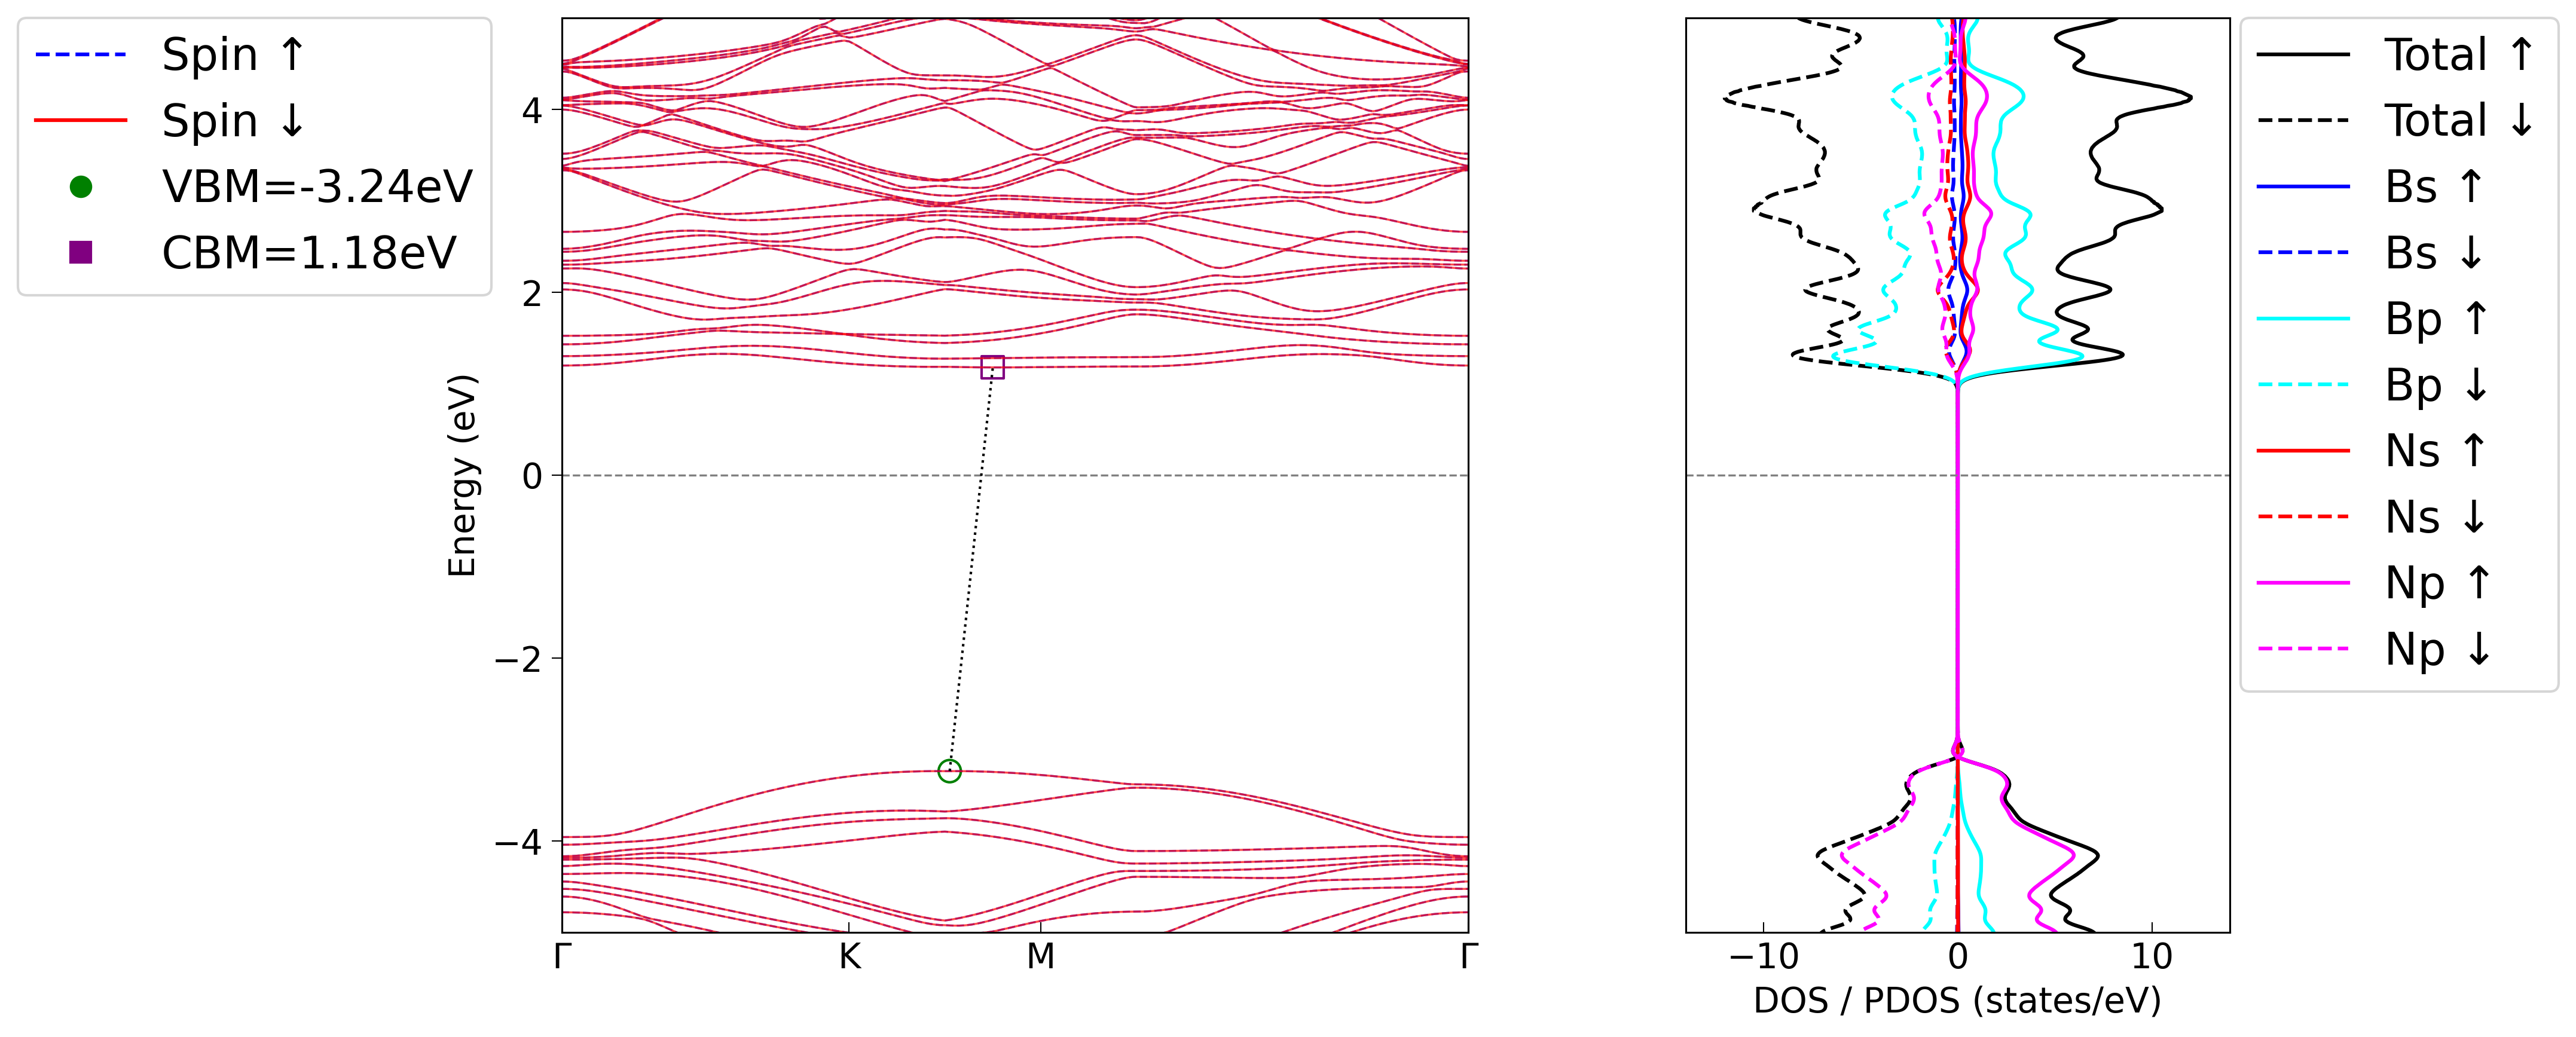
\includegraphics[width=0.95\textwidth]{gambar_hasil/simple_bands_pdos_pure_800K.png}
    \caption{Struktur pita elektronik dan PDOS untuk monolayer hBN murni pada 800 K. Celah pita menyempit menjadi $4.415$ eV.}
    \label{fig:hbn_pure_800K}
\end{figure}

\begin{figure}[htbp!] % PERUBAHAN: Ukuran gambar diperbesar
    \centering
    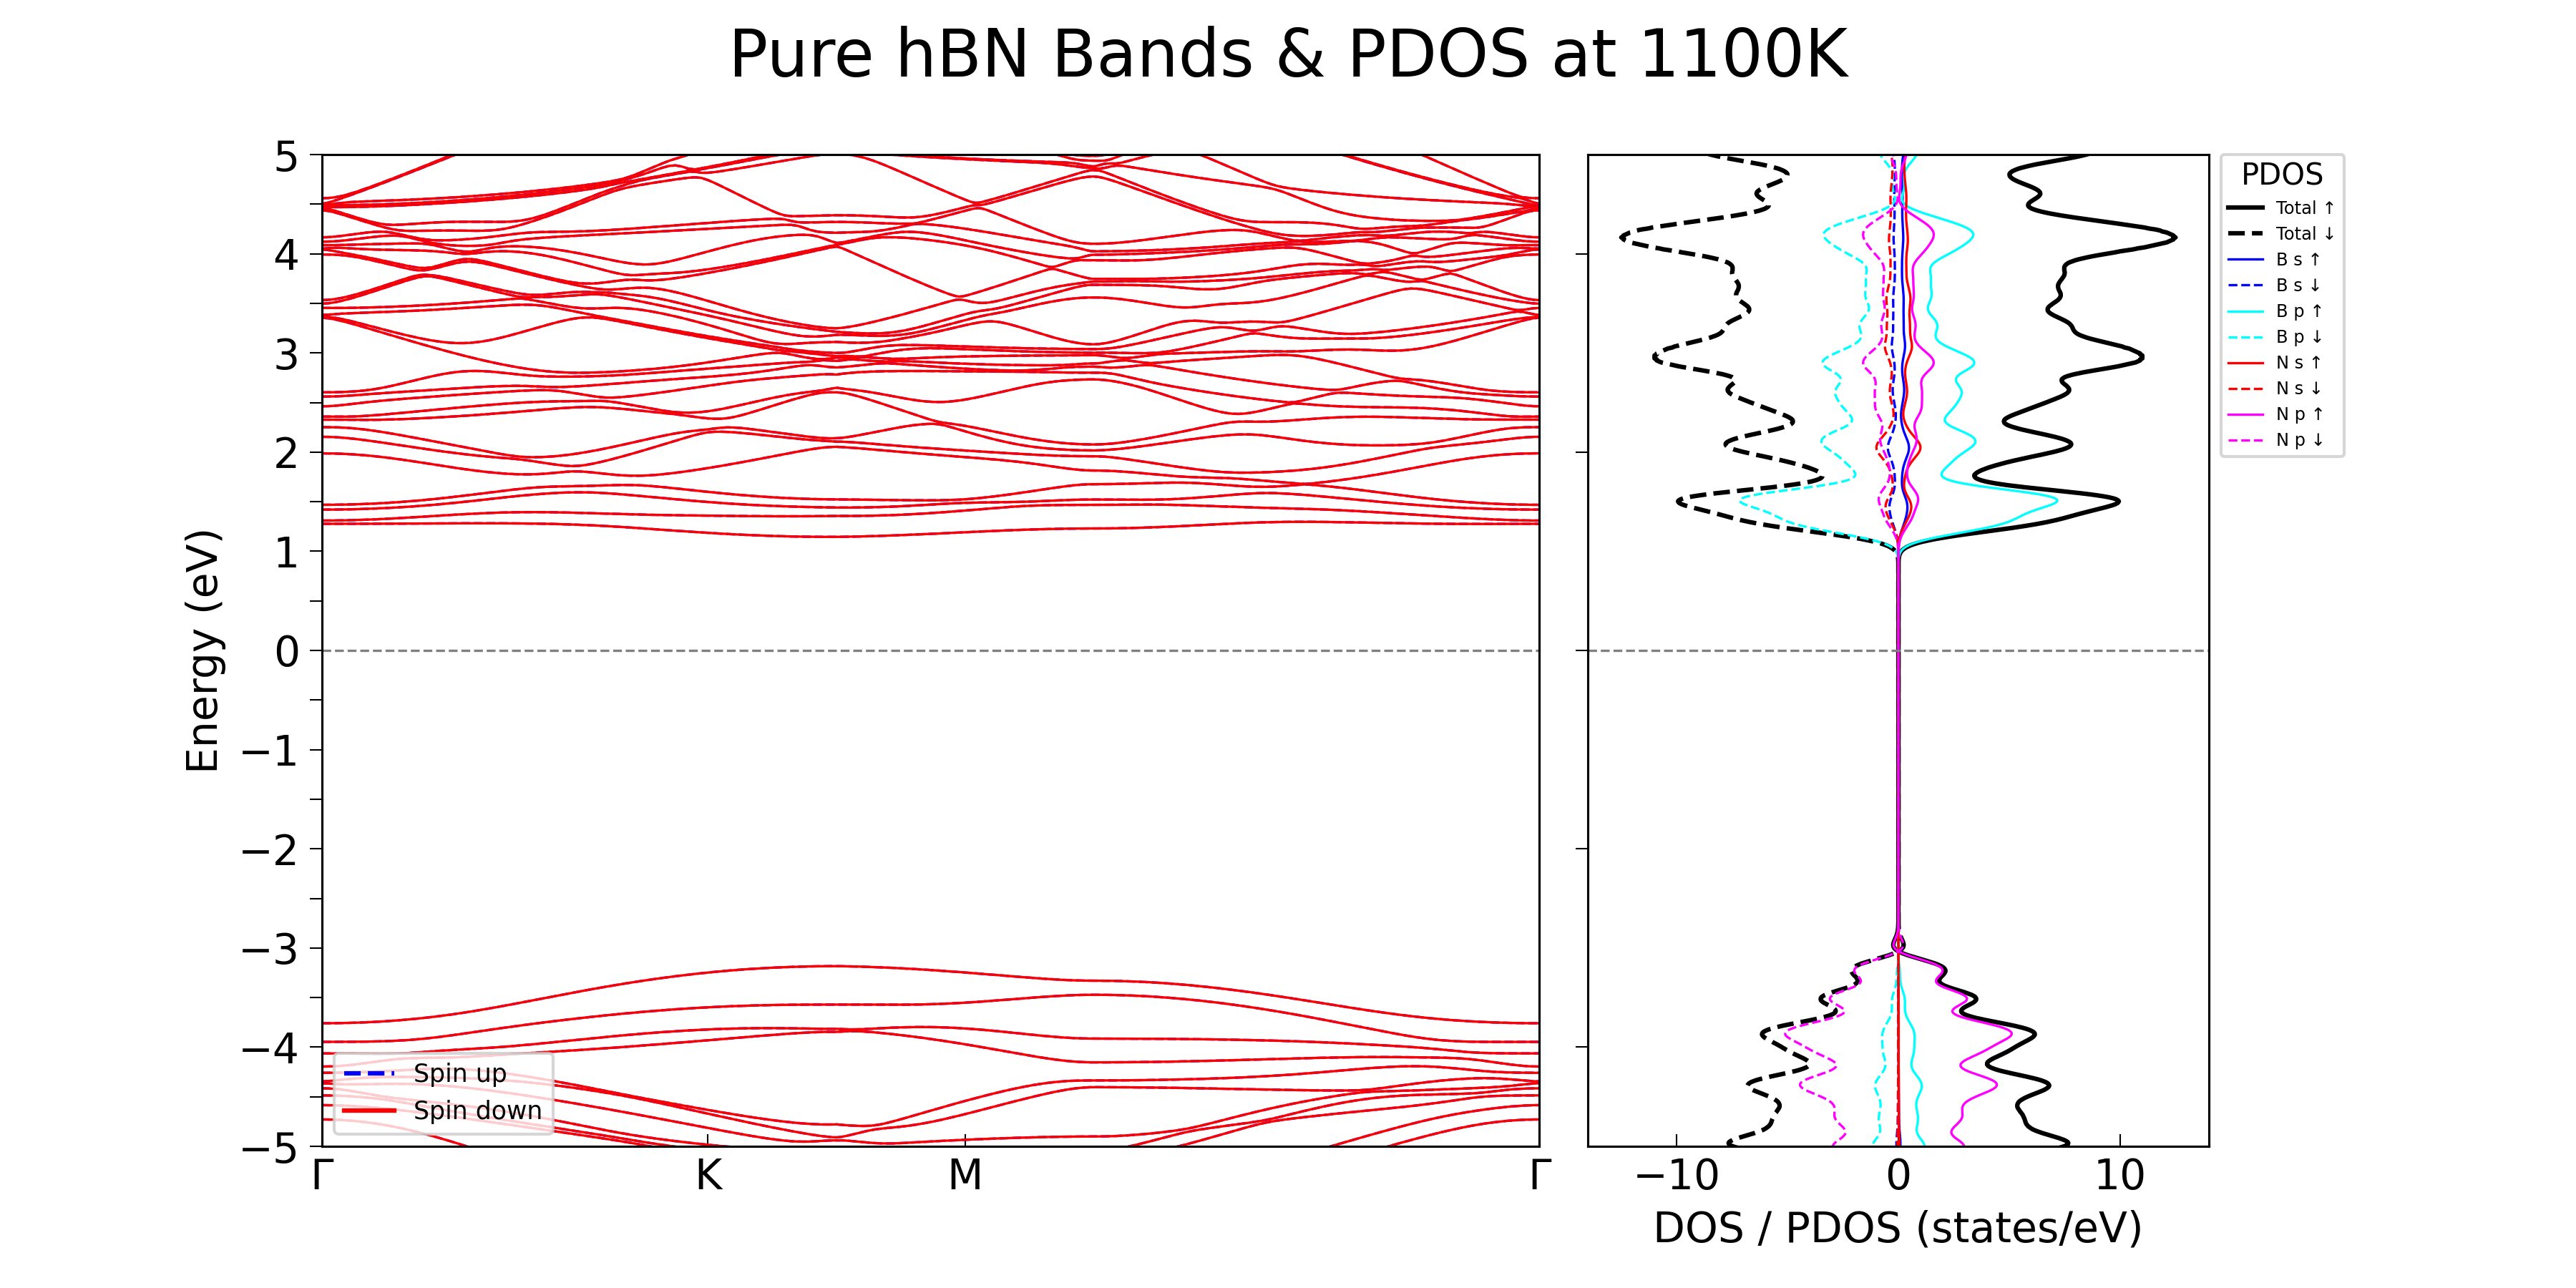
\includegraphics[width=0.95\textwidth]{gambar_hasil/simple_bands_pdos_pure_1100K.png}
    \caption{Struktur pita elektronik dan PDOS untuk monolayer hBN murni pada 1100 K. Celah pita menyempit lebih lanjut menjadi $4.328$ eV.}
    \label{fig:hbn_pure_1100K}
\end{figure}

\begin{figure}[htbp!] % PERUBAHAN: Ukuran gambar diperbesar
    \centering
    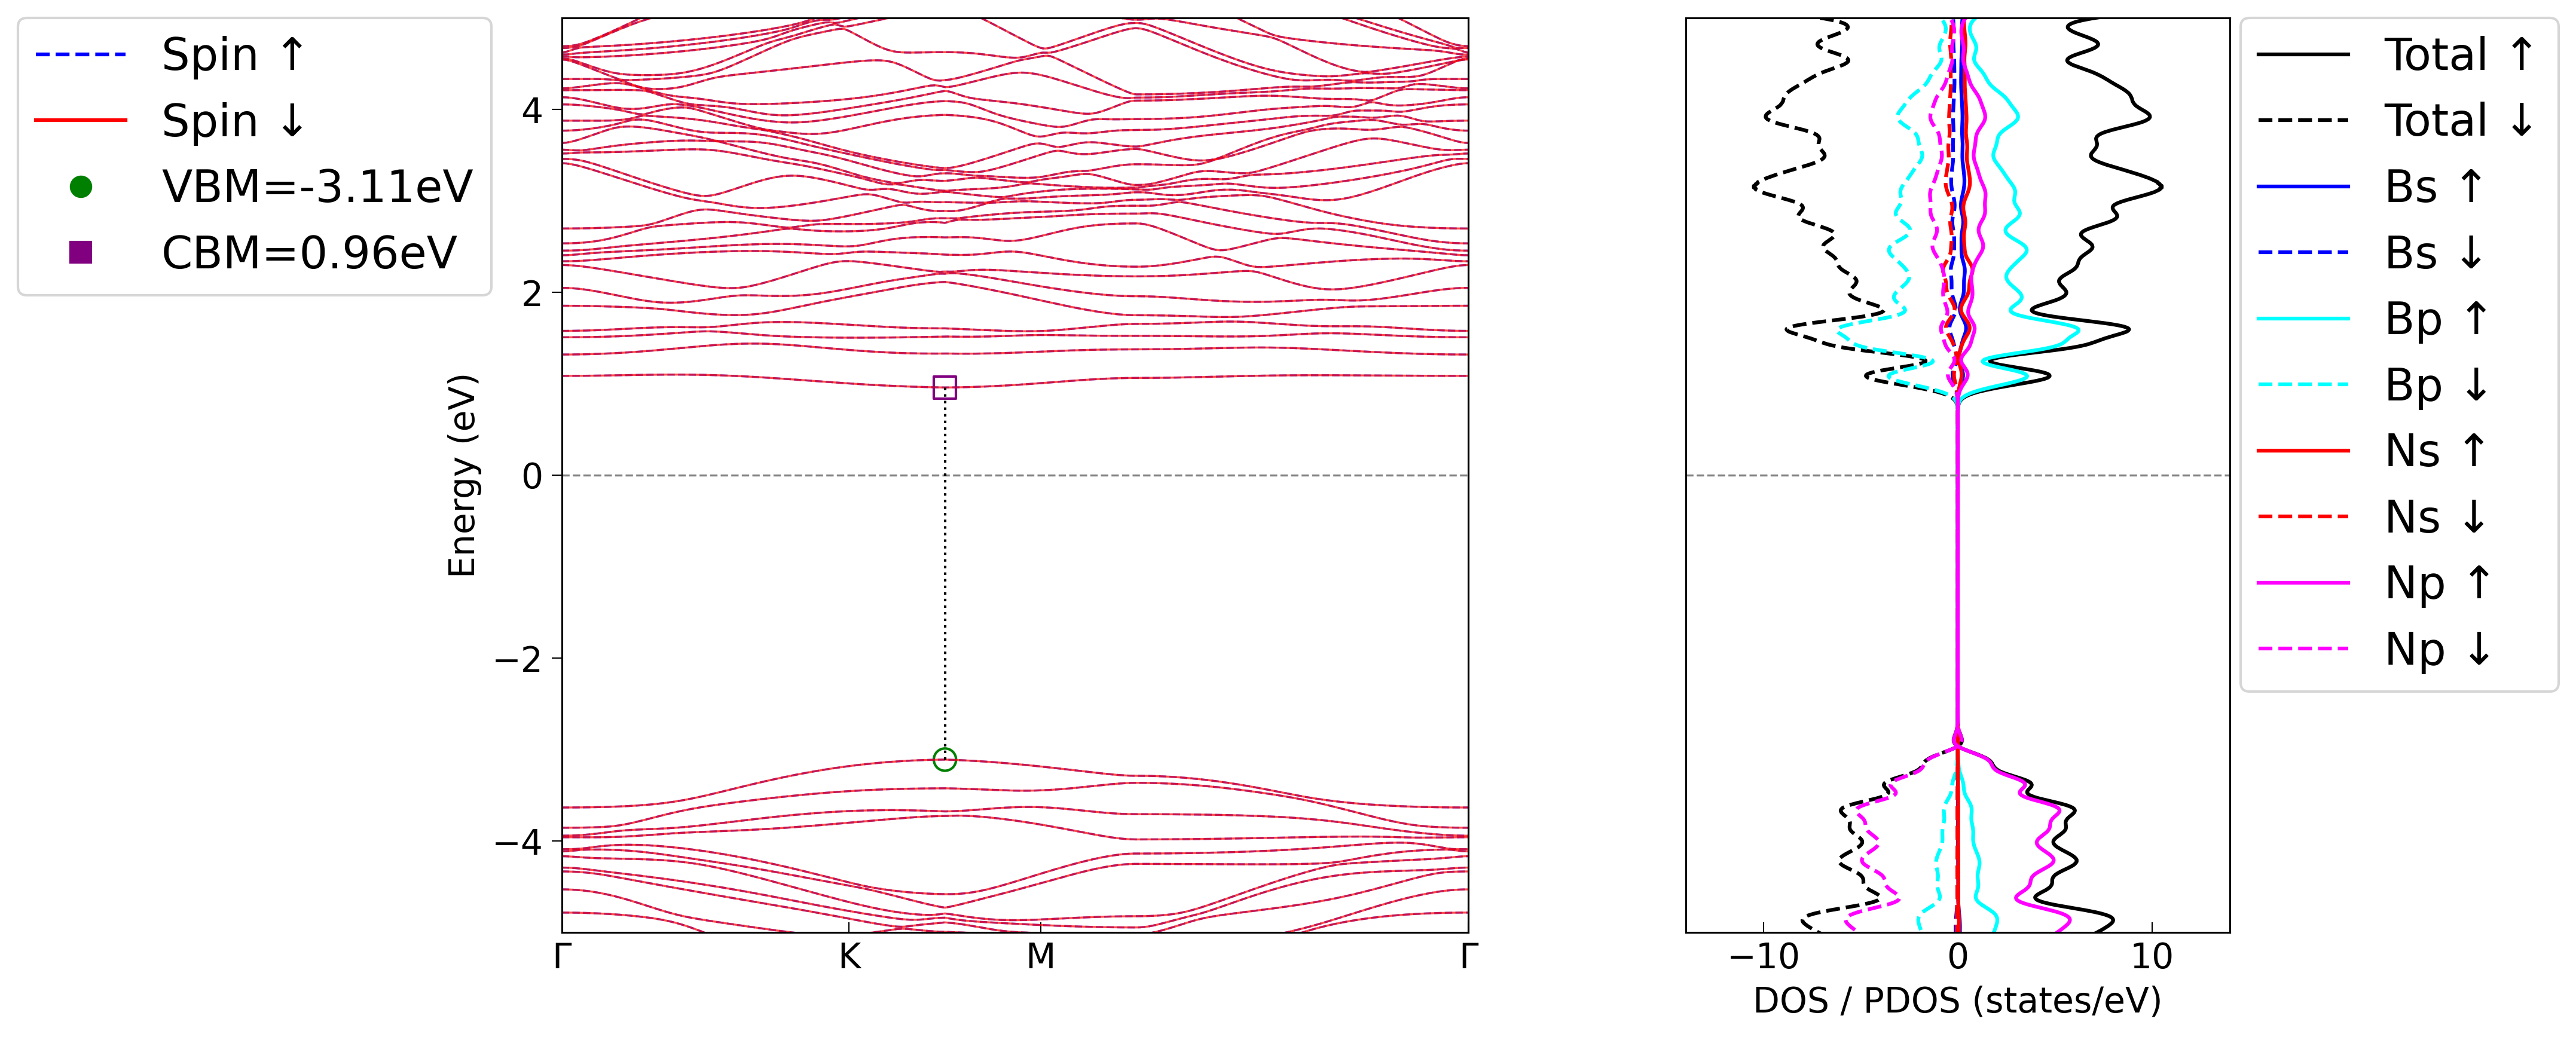
\includegraphics[width=0.95\textwidth]{gambar_hasil/simple_bands_pdos_pure_1225K.png}
    \caption{Struktur pita elektronik dan PDOS untuk monolayer hBN murni pada 1225 K. Celah pita menunjukkan penyempitan signifikan menjadi $4.069$ eV.}
    \label{fig:hbn_pure_1225K}
\end{figure}

Fenomena \emph{redshift} ini adalah manifestasi langsung dari kopling elektron-fonon (EPC).
Pada temperatur hingga, kisi tidak lagi statis; atom-atomnya bervibrasi di sekitar posisi kesetimbangannya. Kuantisasi dari vibrasi kisi ini disebut fonon.
Struktur atomik yang digunakan dalam kalkulasi DFT ini adalah "foto" sesaat atau \emph{snapshot} dari konfigurasi atom yang terdistorsi oleh fonon-fonon ini (pendekatan \emph{frozen-phonon}).
Ketika elektron bergerak melalui kisi yang bergetar ini, energinya direnormalisasi (diubah).
Menurut teori Allen-Heine-Cardona, ada dua kontribusi utama untuk perubahan ini \citep{Allen1983}: (1) koreksi energi-diri Fan-Migdal, di mana elektron "berpakaian" awan fonon virtual, dan (2) kontribusi Debye-Waller, di mana elektron bergerak dalam potensial periodik yang "tercoreng" oleh vibrasi termal.
Kedua efek ini hampir secara universal menyebabkan penurunan energi celah pita pada semikonduktor.
Dengan demikian, penurunan $E_g$ yang diamati dari Gambar \ref{fig:hbn_pure_800K} hingga \ref{fig:hbn_pure_1225K} adalah cerminan dari meningkatnya populasi fonon dan penguatan efek EPC pada temperatur yang lebih tinggi.
Hasil \emph{redshift} yang konsisten ini tampak kontras dengan beberapa laporan eksperimental pada hBN multilayer, yang menunjukkan pergeseran biru (\emph{blueshift}) anomali pada temperatur tinggi \citep{Du2017}.
\emph{Blueshift} tersebut diatribusikan pada dominasi efek Ekspansi Termal Negatif (NTE), di mana kontraksi kisi akibat moda fonon lentur memperlebar celah pita.
Seperti yang telah dibahas pada Bagian \ref{subsec:md_reaxff}, potensial ReaxFF yang digunakan kemungkinan besar tidak menangkap mekanisme NTE ini.
Akibatnya, simulasi ini secara efektif mengisolasi kontribusi dari EPC. Oleh karena itu, \emph{redshift} yang diamati bukanlah sebuah kontradiksi, melainkan hasil yang konsisten secara internal dengan fisika yang "diizinkan" oleh model: tanpa adanya mekanisme \emph{blueshift} dari NTE, mekanisme \emph{redshift} dari EPC menjadi dominan dan secara akurat ditangkap oleh kalkulasi DFT.

\subsection{Analisis Visual Kerapatan Muatan dan Spin}
\label{subsec:hbn_pure_density_analysis}
Untuk melengkapi analisis struktur pita, visualisasi distribusi elektron dalam ruang nyata memberikan wawasan kualitatif yang kuat.
Gambar \ref{fig:hbn_pure_density} menyajikan plot kerapatan muatan dan kerapatan spin untuk sistem hBN murni pada setiap temperatur.

%%%%%%%%%%%%%%%%%%%%%%%%%%%%%%%%%%%%%%%%%%%%%%%%%%%%%%%%%%%%%%%%%%%%%%
% PERBAIKAN GAMBAR: KERAPATAN MUATAN/SPIN (MURNI)
% Permintaan: Membuat gambar lebih besar.
% Solusi: Menggunakan lebar 0.49\textwidth untuk setiap subfigure memastikan
% gambar mengisi lebar teks secara horizontal, memberikan ukuran maksimal
% untuk tata letak dua kolom.
%%%%%%%%%%%%%%%%%%%%%%%%%%%%%%%%%%%%%%%%%%%%%%%%%%%%%%%%%%%%%%%%%%%%%%
\begin{figure}[htbp!]
  \centering
  \begin{subfigure}[b]{0.49\textwidth}
    \centering
    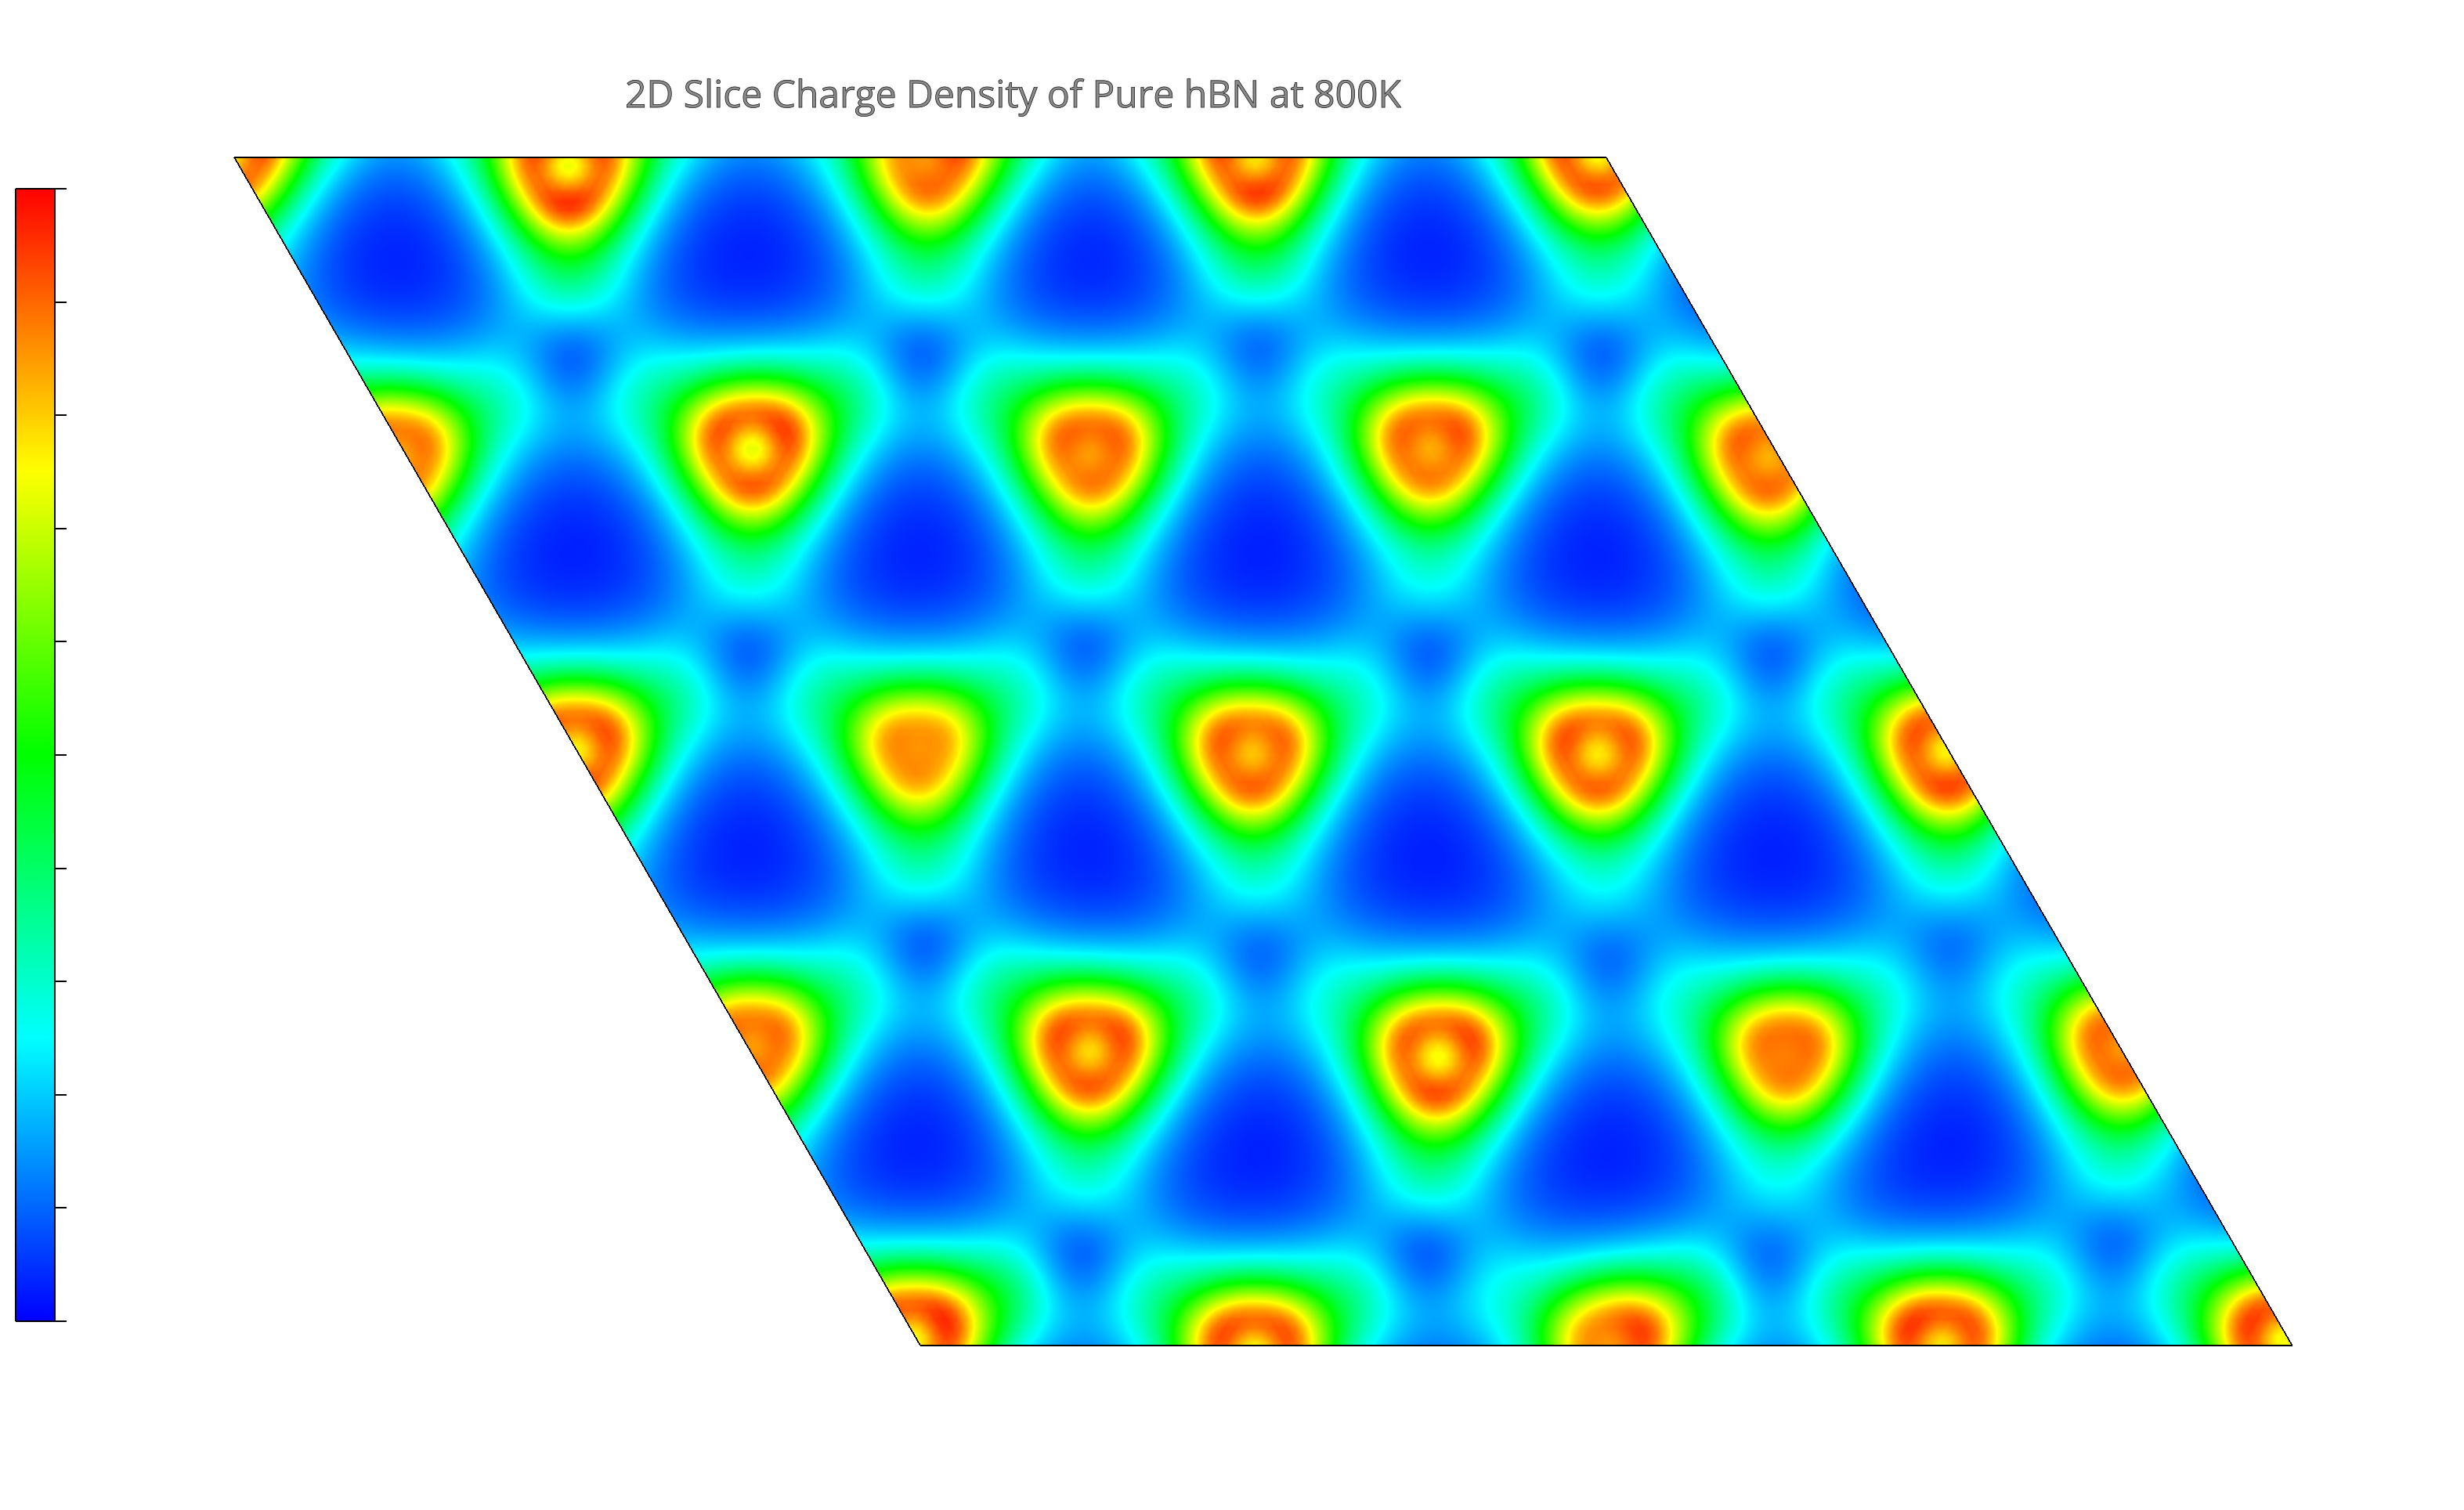
\includegraphics[width=\linewidth]{hBN_rho_pure_800K.png}
    \caption{Kerapatan Muatan, 800 K}
    \label{subfig:rho_pure_800k}
  \end{subfigure}\hfill
  \begin{subfigure}[b]{0.49\textwidth}
    \centering
    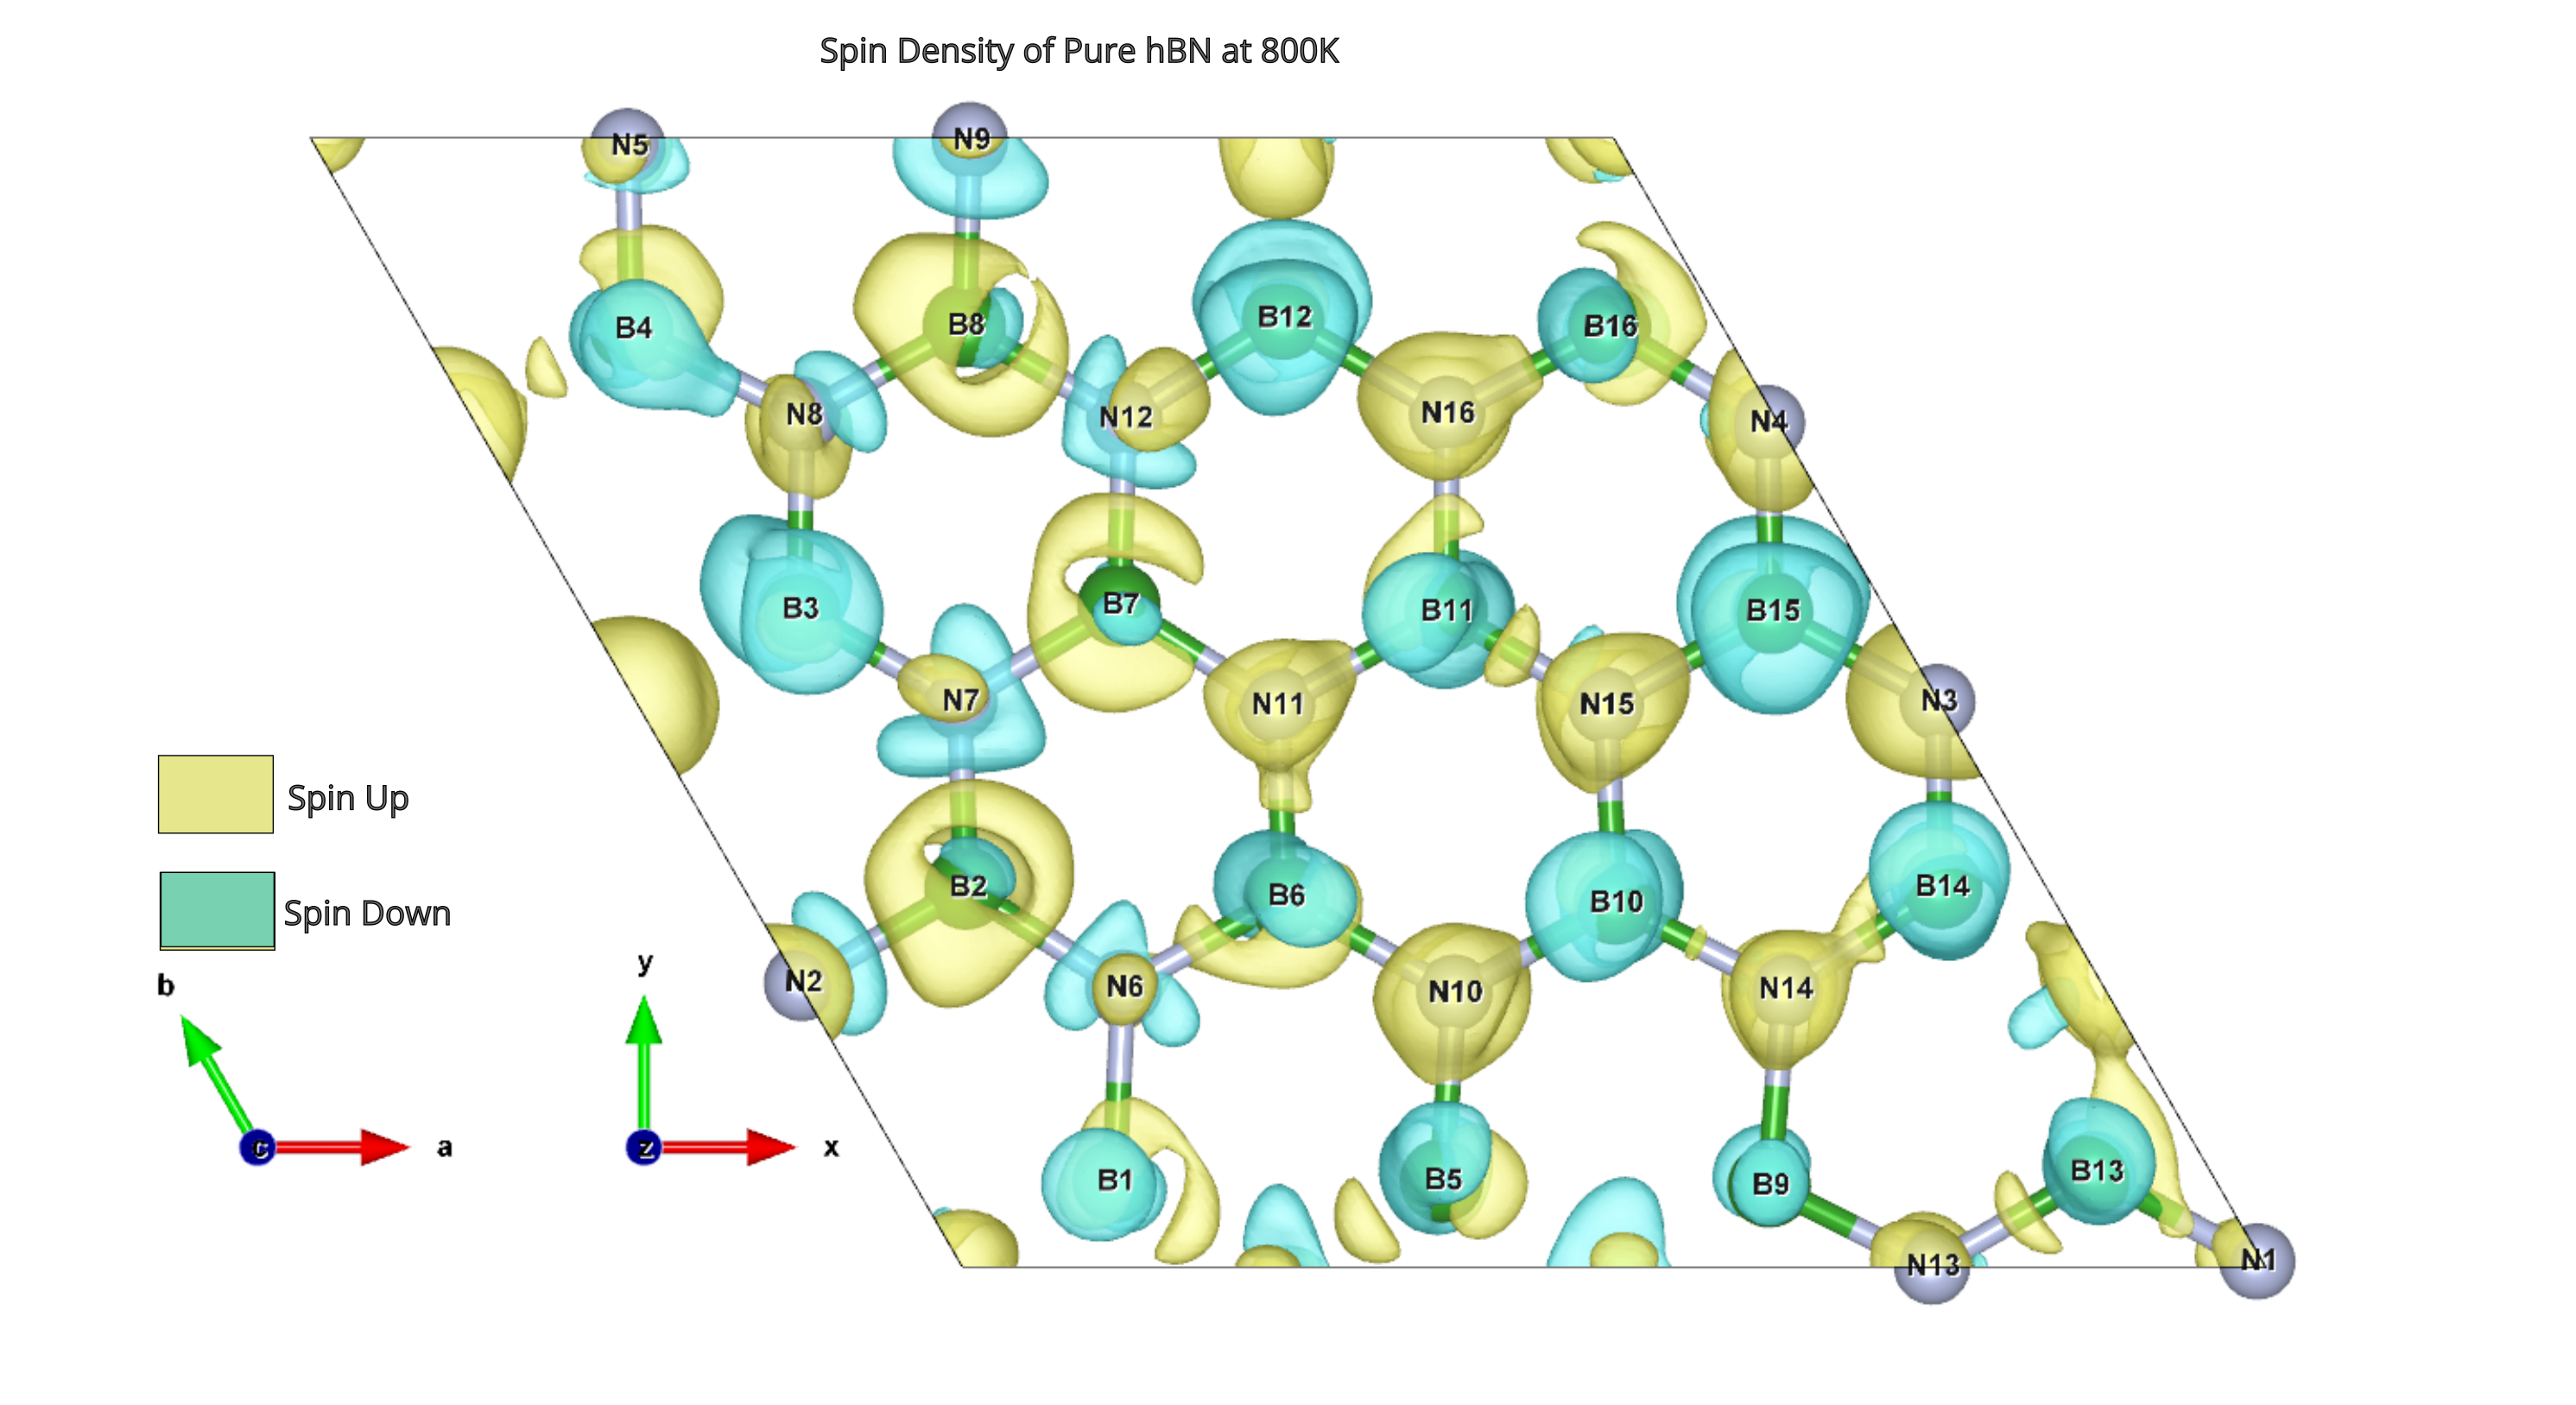
\includegraphics[width=\linewidth]{hBN_spin_pure_800K.png}
    \caption{Kerapatan Spin, 800 K}
    \label{subfig:spin_pure_800k}
  \end{subfigure}
  \vspace{1em}

  \begin{subfigure}[b]{0.49\textwidth}
    \centering
    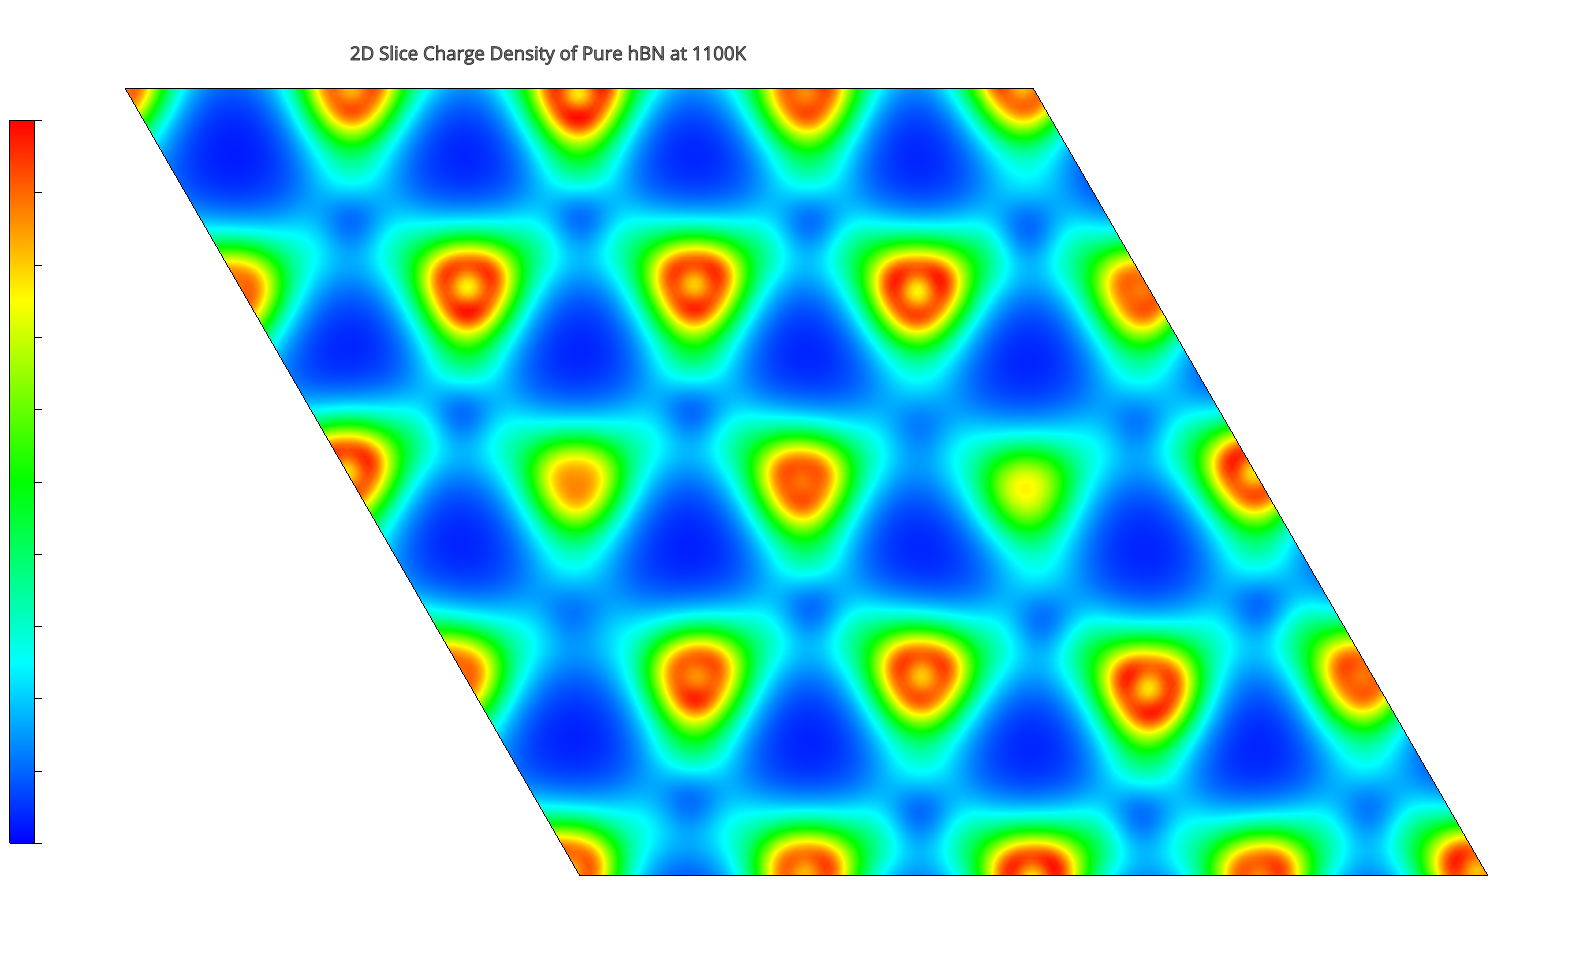
\includegraphics[width=\linewidth]{hBN_rho_pure_1100K.png}
    \caption{Kerapatan Muatan, 1100 K}
    \label{subfig:rho_pure_1100k}
  \end{subfigure}\hfill
  \begin{subfigure}[b]{0.49\textwidth}
    \centering
    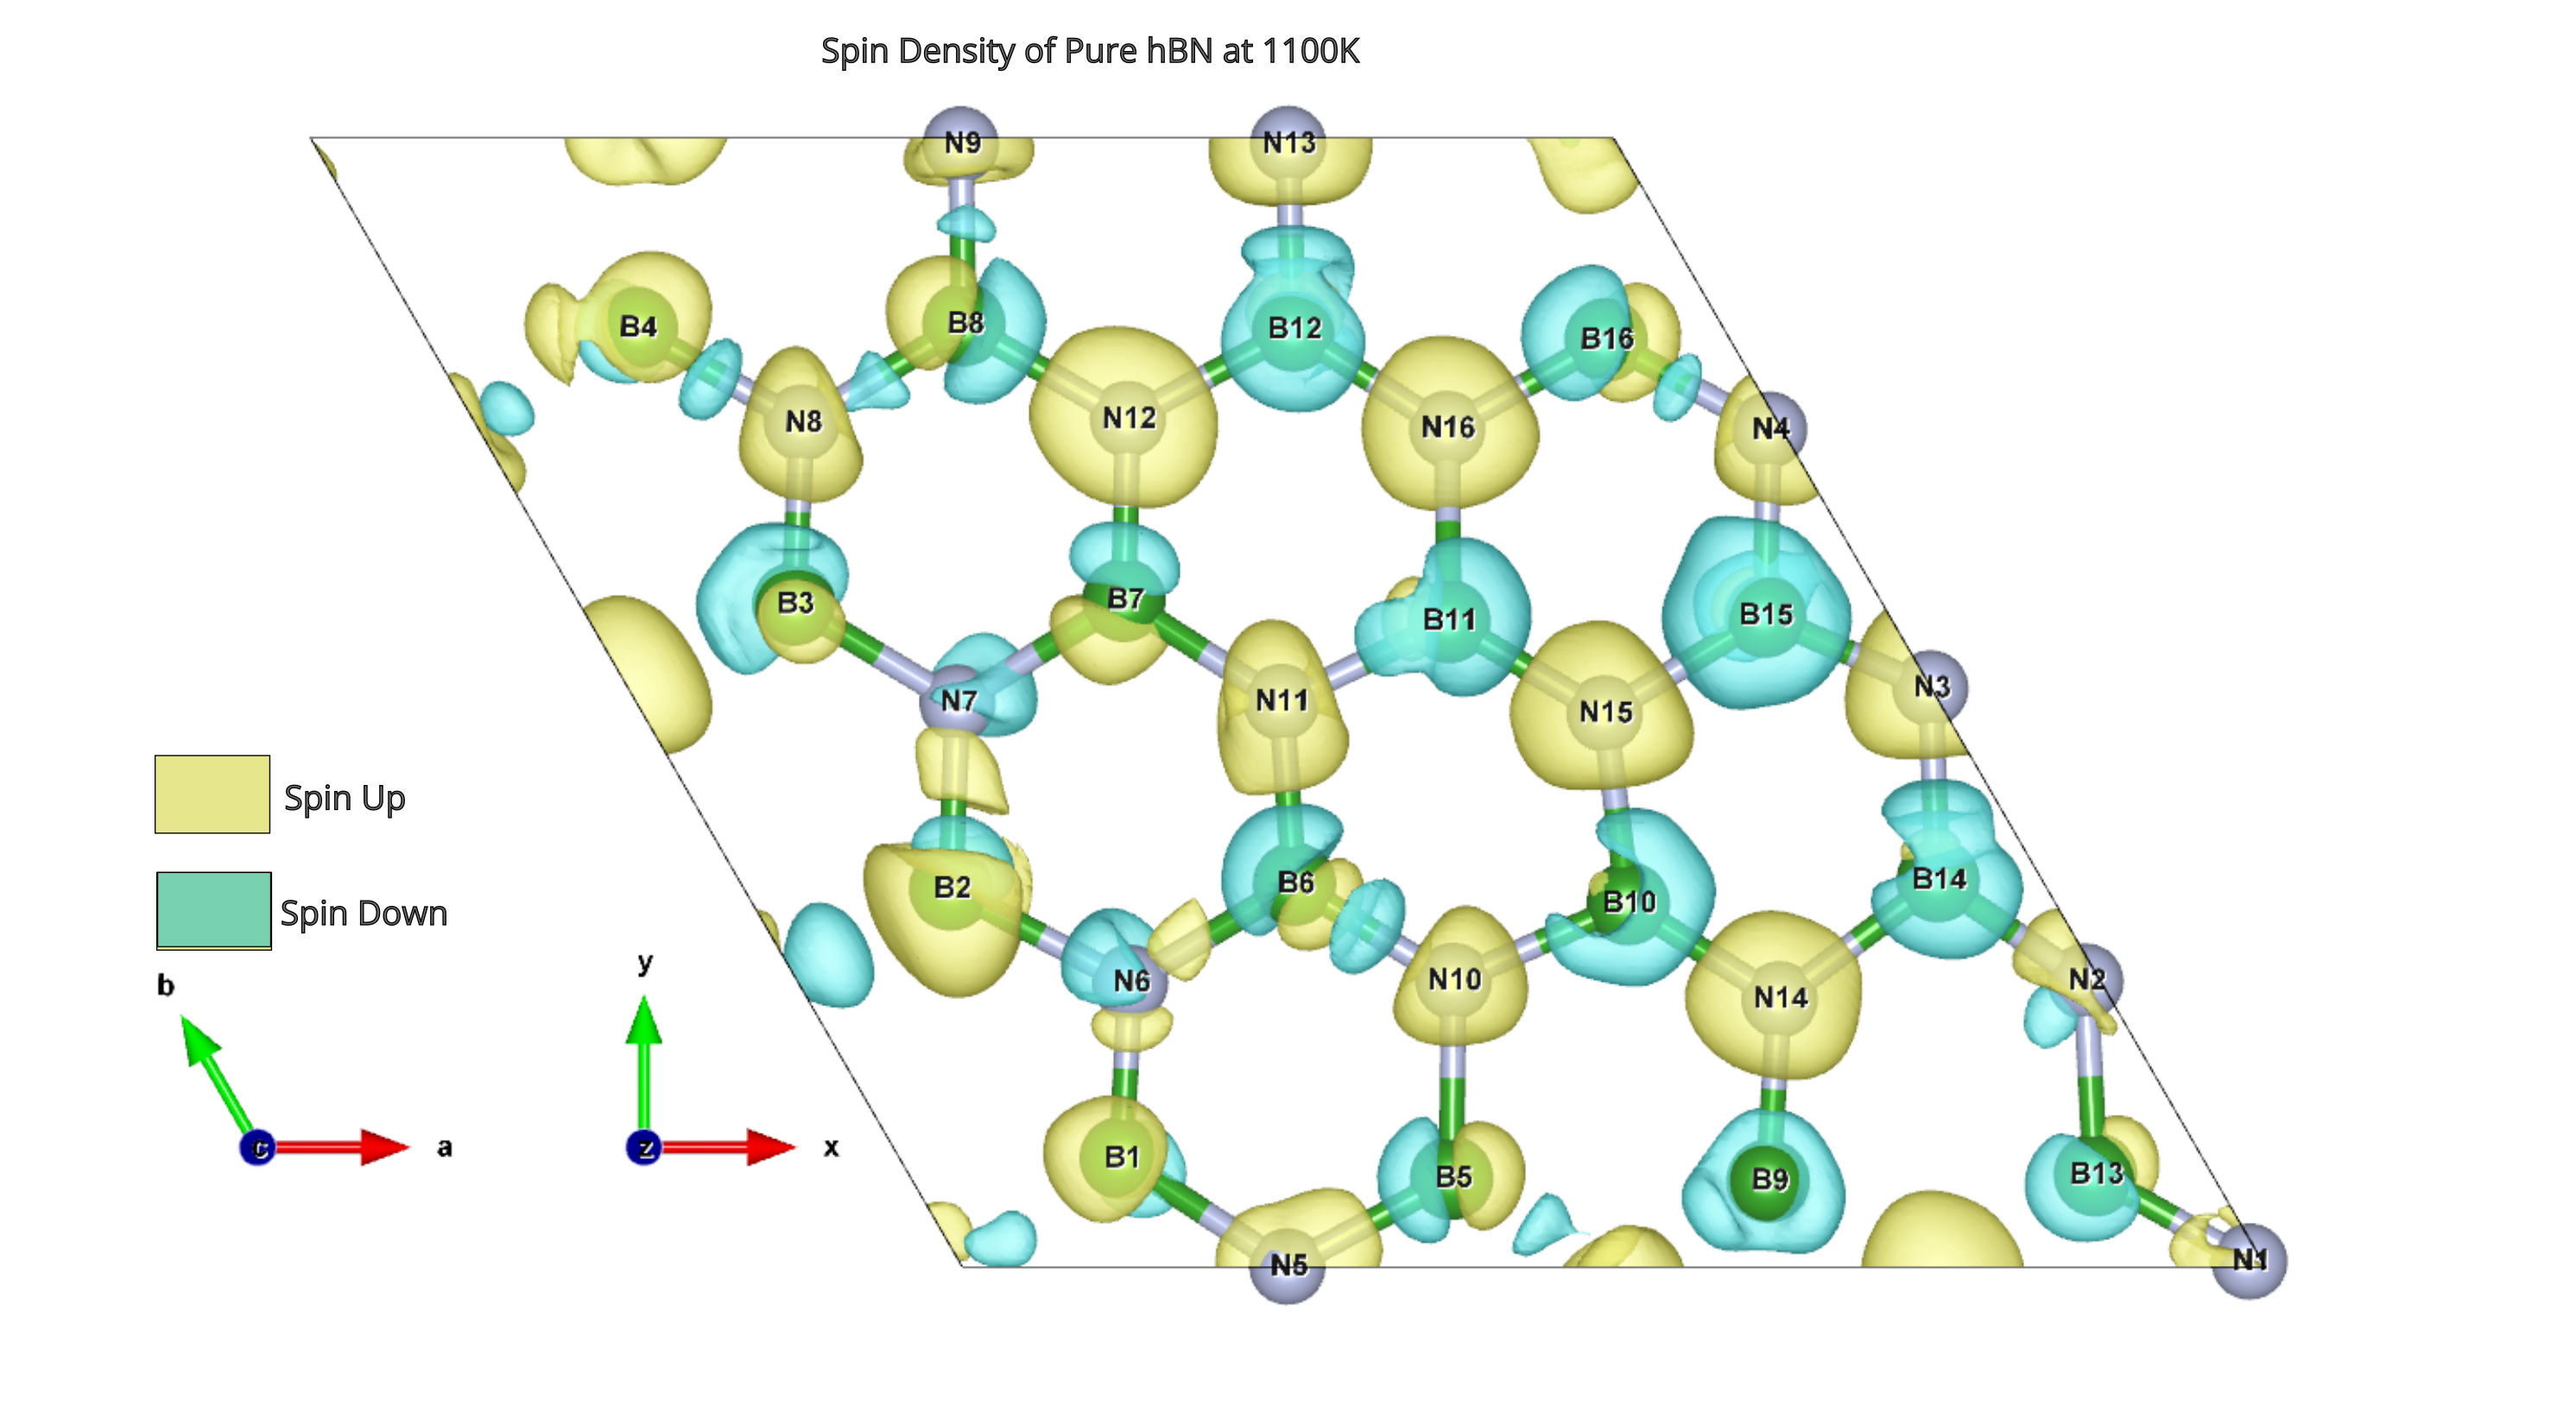
\includegraphics[width=\linewidth]{hBN_spin_pure_1100K.png}
    \caption{Kerapatan Spin, 1100 K}
    \label{subfig:spin_pure_1100k}
  \end{subfigure}
  \vspace{1em}

  \begin{subfigure}[b]{0.49\textwidth}
    \centering
    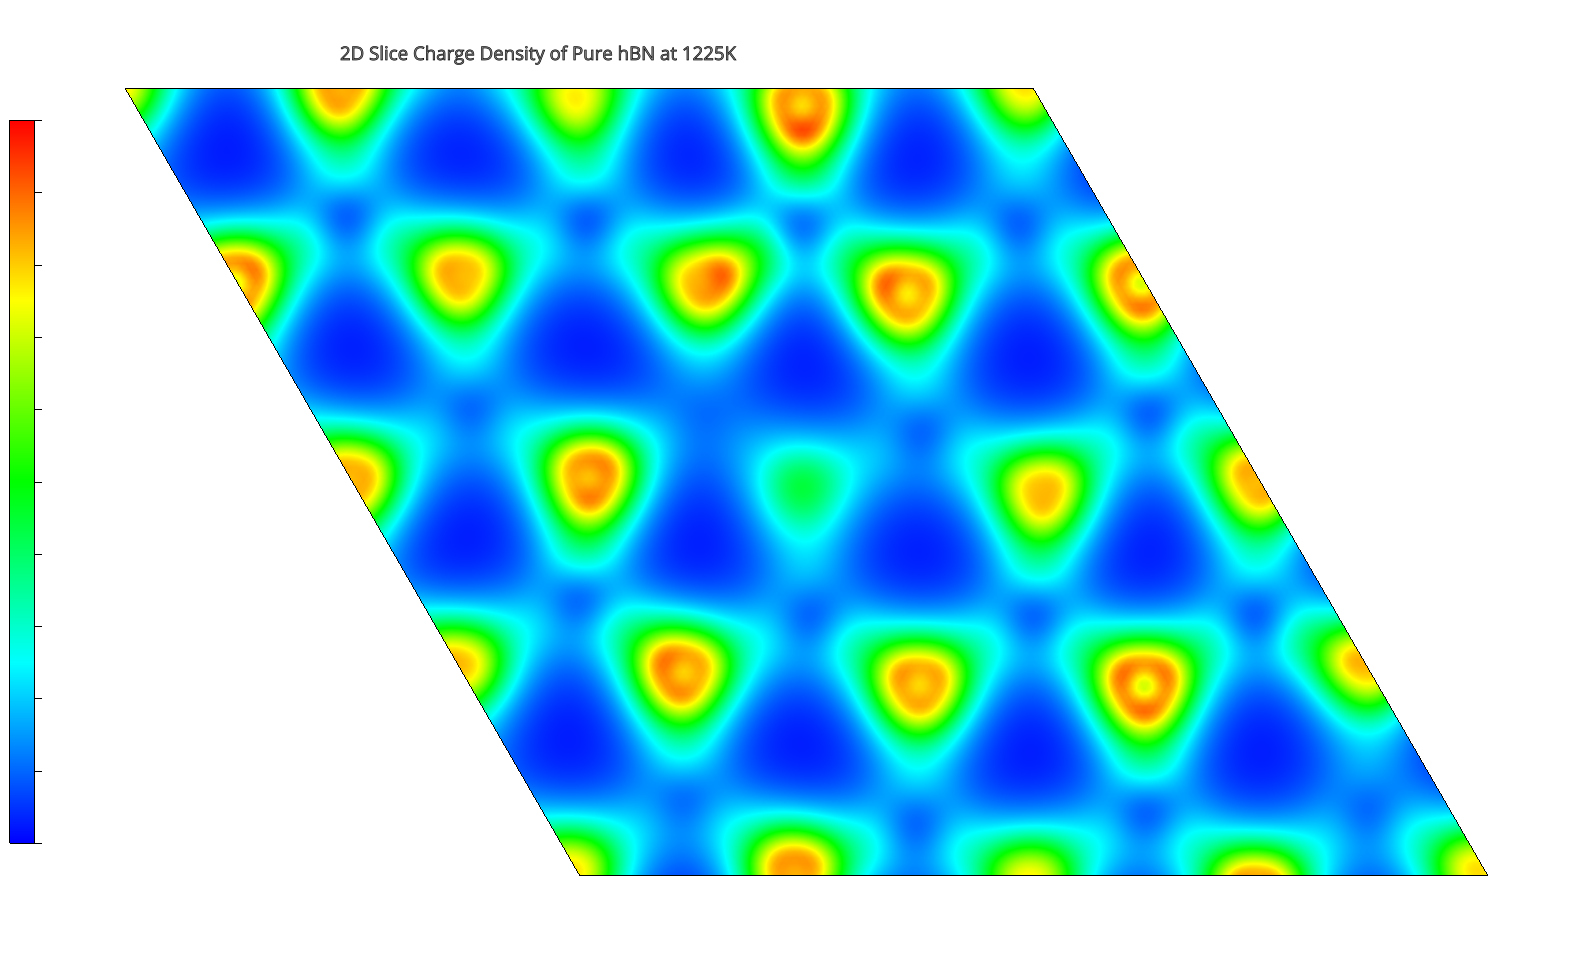
\includegraphics[width=\linewidth]{hBN_rho_pure_1225K.png}
    \caption{Kerapatan Muatan, 1225 K}
    \label{subfig:rho_pure_1225k}
  \end{subfigure}\hfill
  \begin{subfigure}[b]{0.49\textwidth}
    \centering
    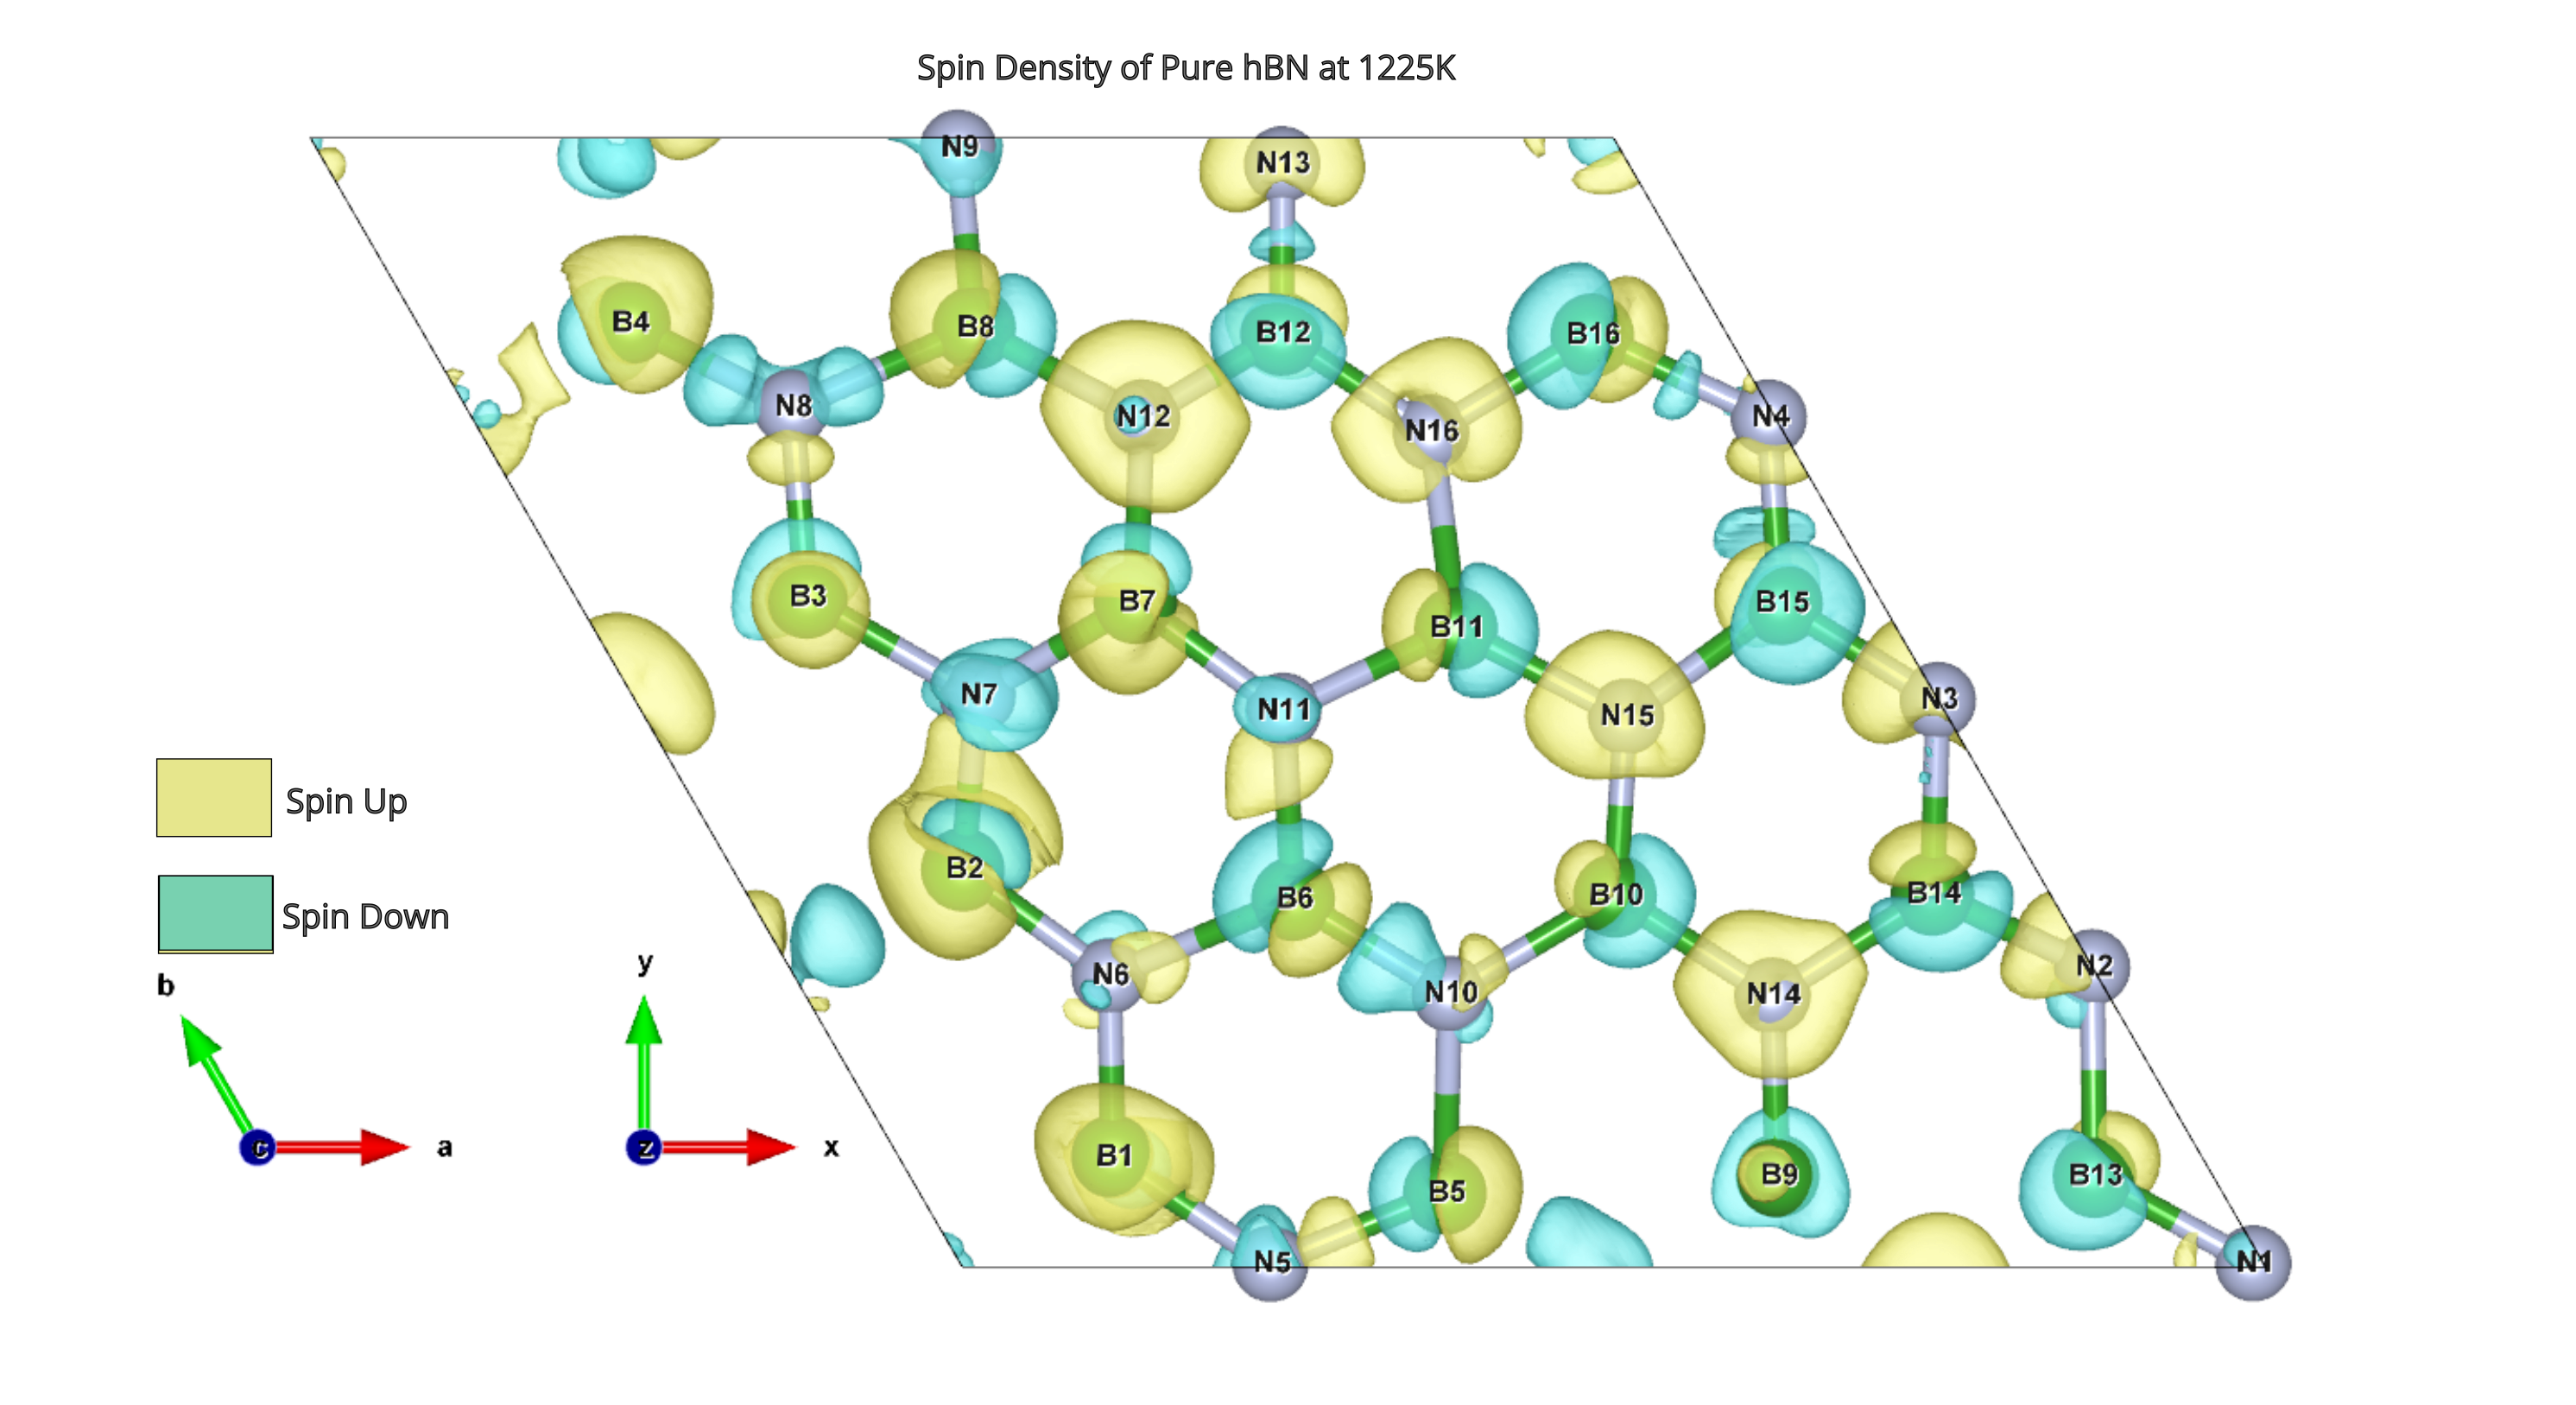
\includegraphics[width=\linewidth]{hBN_spin_pure_1225K.png}
    \caption{Kerapatan Spin, 1225 K}
    \label{subfig:spin_pure_1225k}
  \end{subfigure}

  \caption{Visualisasi 2D dari kerapatan muatan total (kiri) dan kerapatan spin (kanan) untuk monolayer hBN murni pada 800 K, 1100 K, dan 1225 K. Warna merah pada kerapatan muatan menunjukkan akumulasi elektron, sedangkan warna biru menunjukkan deplesi. Untuk kerapatan spin, warna biru menunjukkan spin down dan warna kuning menunjukan spin up.}
  \label{fig:hbn_pure_density}
\end{figure}

Plot kerapatan muatan (Gambar \ref{fig:hbn_pure_density}a, c, e) secara konsisten menunjukkan akumulasi kerapatan elektron yang signifikan di sekitar situs atom nitrogen (merah) dan deplesi di sekitar situs atom boron (biru).
Ini adalah bukti visual langsung dari sifat ikatan kovalen polar yang kuat dalam hBN, yang timbul dari perbedaan elektronegativitas yang besar antara B dan N. Meskipun struktur atomik mengalami distorsi termal dan \emph{rippling} (seperti yang ditunjukkan pada Gambar \ref{fig:md_structures_per_condition}), distribusi muatan dalam bidang ini tetap sangat teratur dan periodik.
Hal ini mencerminkan ketahanan kerangka ikatan $\sigma$ yang kuat, yang mendefinisikan sifat elektronik dasar material.
Yang tidak kalah penting adalah analisis kerapatan spin (Gambar \ref{fig:hbn_pure_density}b, d, f).
Untuk semua temperatur yang diselidiki, plot menunjukkan nilai nol yang seragam di seluruh supercell.
Ini adalah konfirmasi visual yang definitif bahwa hBN murni adalah material non-magnetik.
Tidak adanya polarisasi spin (perbedaan antara kerapatan elektron spin-atas dan spin-bawah) secara sempurna sejalan dengan struktur pita yang simetris untuk kedua kanal spin (misalnya, Gambar \ref{fig:hbn_pure_1225K}) dan nilai magnetisasi total nol yang dilaporkan dalam Tabel \ref{tab:hbn_murni_suhu}.
Hasil ini menegaskan bahwa agitasi termal, meskipun cukup untuk menyebabkan distorsi kisi yang signifikan dan merenormalisasi celah pita, tidak cukup untuk memecah simetri spin dan menginduksi momen magnetik.
Pengamatan ini menetapkan dasar referensi yang krusial untuk mengevaluasi dampak pengenalan cacat.

\section{Rekayasa Sifat Elektronik dan Magnetik Melalui Cacat Antisite}
\label{sec:hbn_defek}
Kehadiran cacat titik secara fundamental mengubah lanskap elektronik material, seringkali mengintroduksi perilaku yang tidak ada pada material induknya.
Bagian ini membahas bagaimana dua jenis cacat antisite, N\textsubscript{B} (Nitrogen pada situs Boron) dan B\textsubscript{N} (Boron pada situs Nitrogen), secara dramatis memodulasi sifat elektronik dan magnetik monolayer hBN sebagai respons terhadap temperatur.
\subsection{Cacat N\textsubscript{B}: Pergeseran Biru Anomali dan Kopling Elektron-Fonon Terlokalisasi}
\label{subsec:hbn_defek_nb}
Introduksi cacat antisite N\textsubscript{B} menyebabkan perubahan drastis pada struktur elektronik.
Seperti yang ditunjukkan pada Gambar \ref{fig:hbn_NN_800K}, cacat ini menciptakan tingkat-tingkat energi baru yang terlokalisasi di dalam celah pita intrinsik hBN, secara signifikan mengurangi celah pita efektif menjadi $0.694$ eV pada 800 K.
\begin{table}[htbp!] % STANDARISASI: Menggunakan [htbp!]
  \centering
  \caption{Sifat Elektronik Monolayer hBN dengan Cacat Antisite N\textsubscript{B} sebagai Fungsi Temperatur.}
  \label{tab:hbn_defek_nb}
  \begin{tabular}{lcccccc}
    \toprule
    Temperatur & VBM & CBM & $E_g$ & $E_F$ & Magnetisasi & Magnetisasi \\
    (K) & (eV) & (eV) & (eV) & (eV) & Total ($\mu_B$) & Absolut ($\mu_B$) \\
    \midrule
    800  & -0.448 &  0.246 & 0.694 & -2.538 & 0.000 & 0.000 \\
    1100 & -0.666 &  0.423 & 1.089 & -2.682 & 0.000 & 0.000 \\
    1225 & -0.732 &  0.482 & 1.214 & -2.237 & 0.000 & 0.010 \\
    \bottomrule
  \end{tabular}
\end{table}

\begin{figure}[htbp!] % PERUBAHAN: Ukuran gambar diperbesar
    \centering
    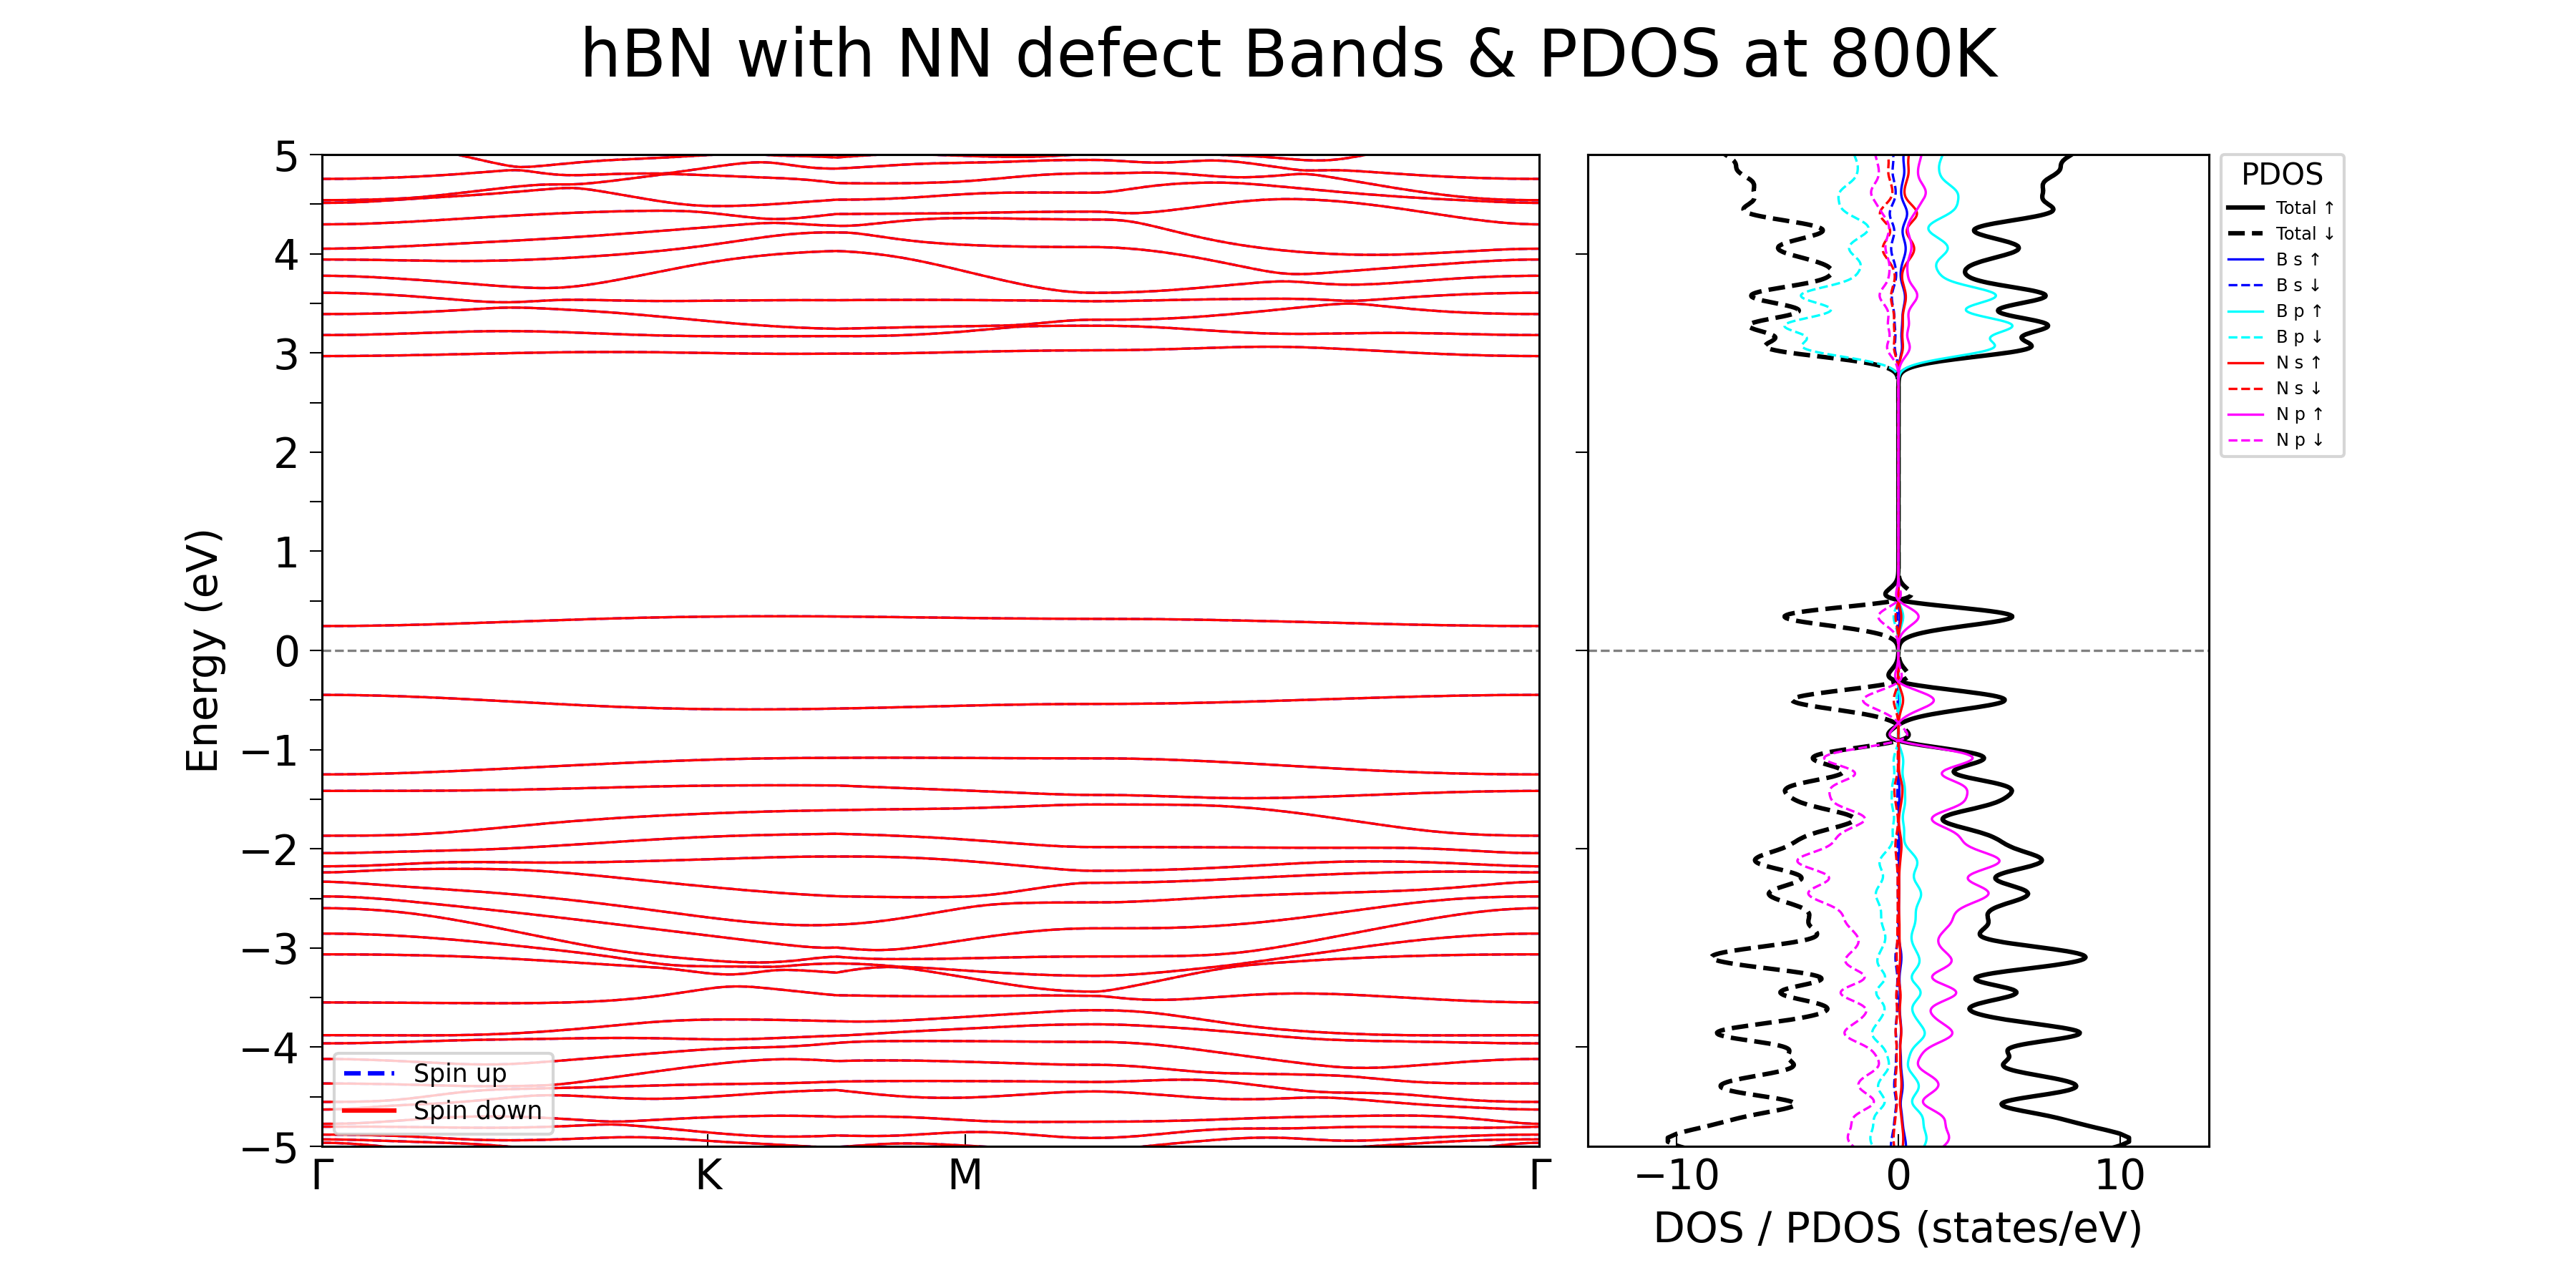
\includegraphics[width=0.95\textwidth]{gambar_hasil/simple_bands_pdos_NN_800K.png}
    \caption{Struktur pita elektronik dan PDOS untuk monolayer hBN dengan cacat N\textsubscript{B} pada 800 K. Terlihat tingkat cacat di dalam celah pita.}
    \label{fig:hbn_NN_800K}
\end{figure}
\begin{figure}[htbp!] % PERUBAHAN: Ukuran gambar diperbesar
    \centering
    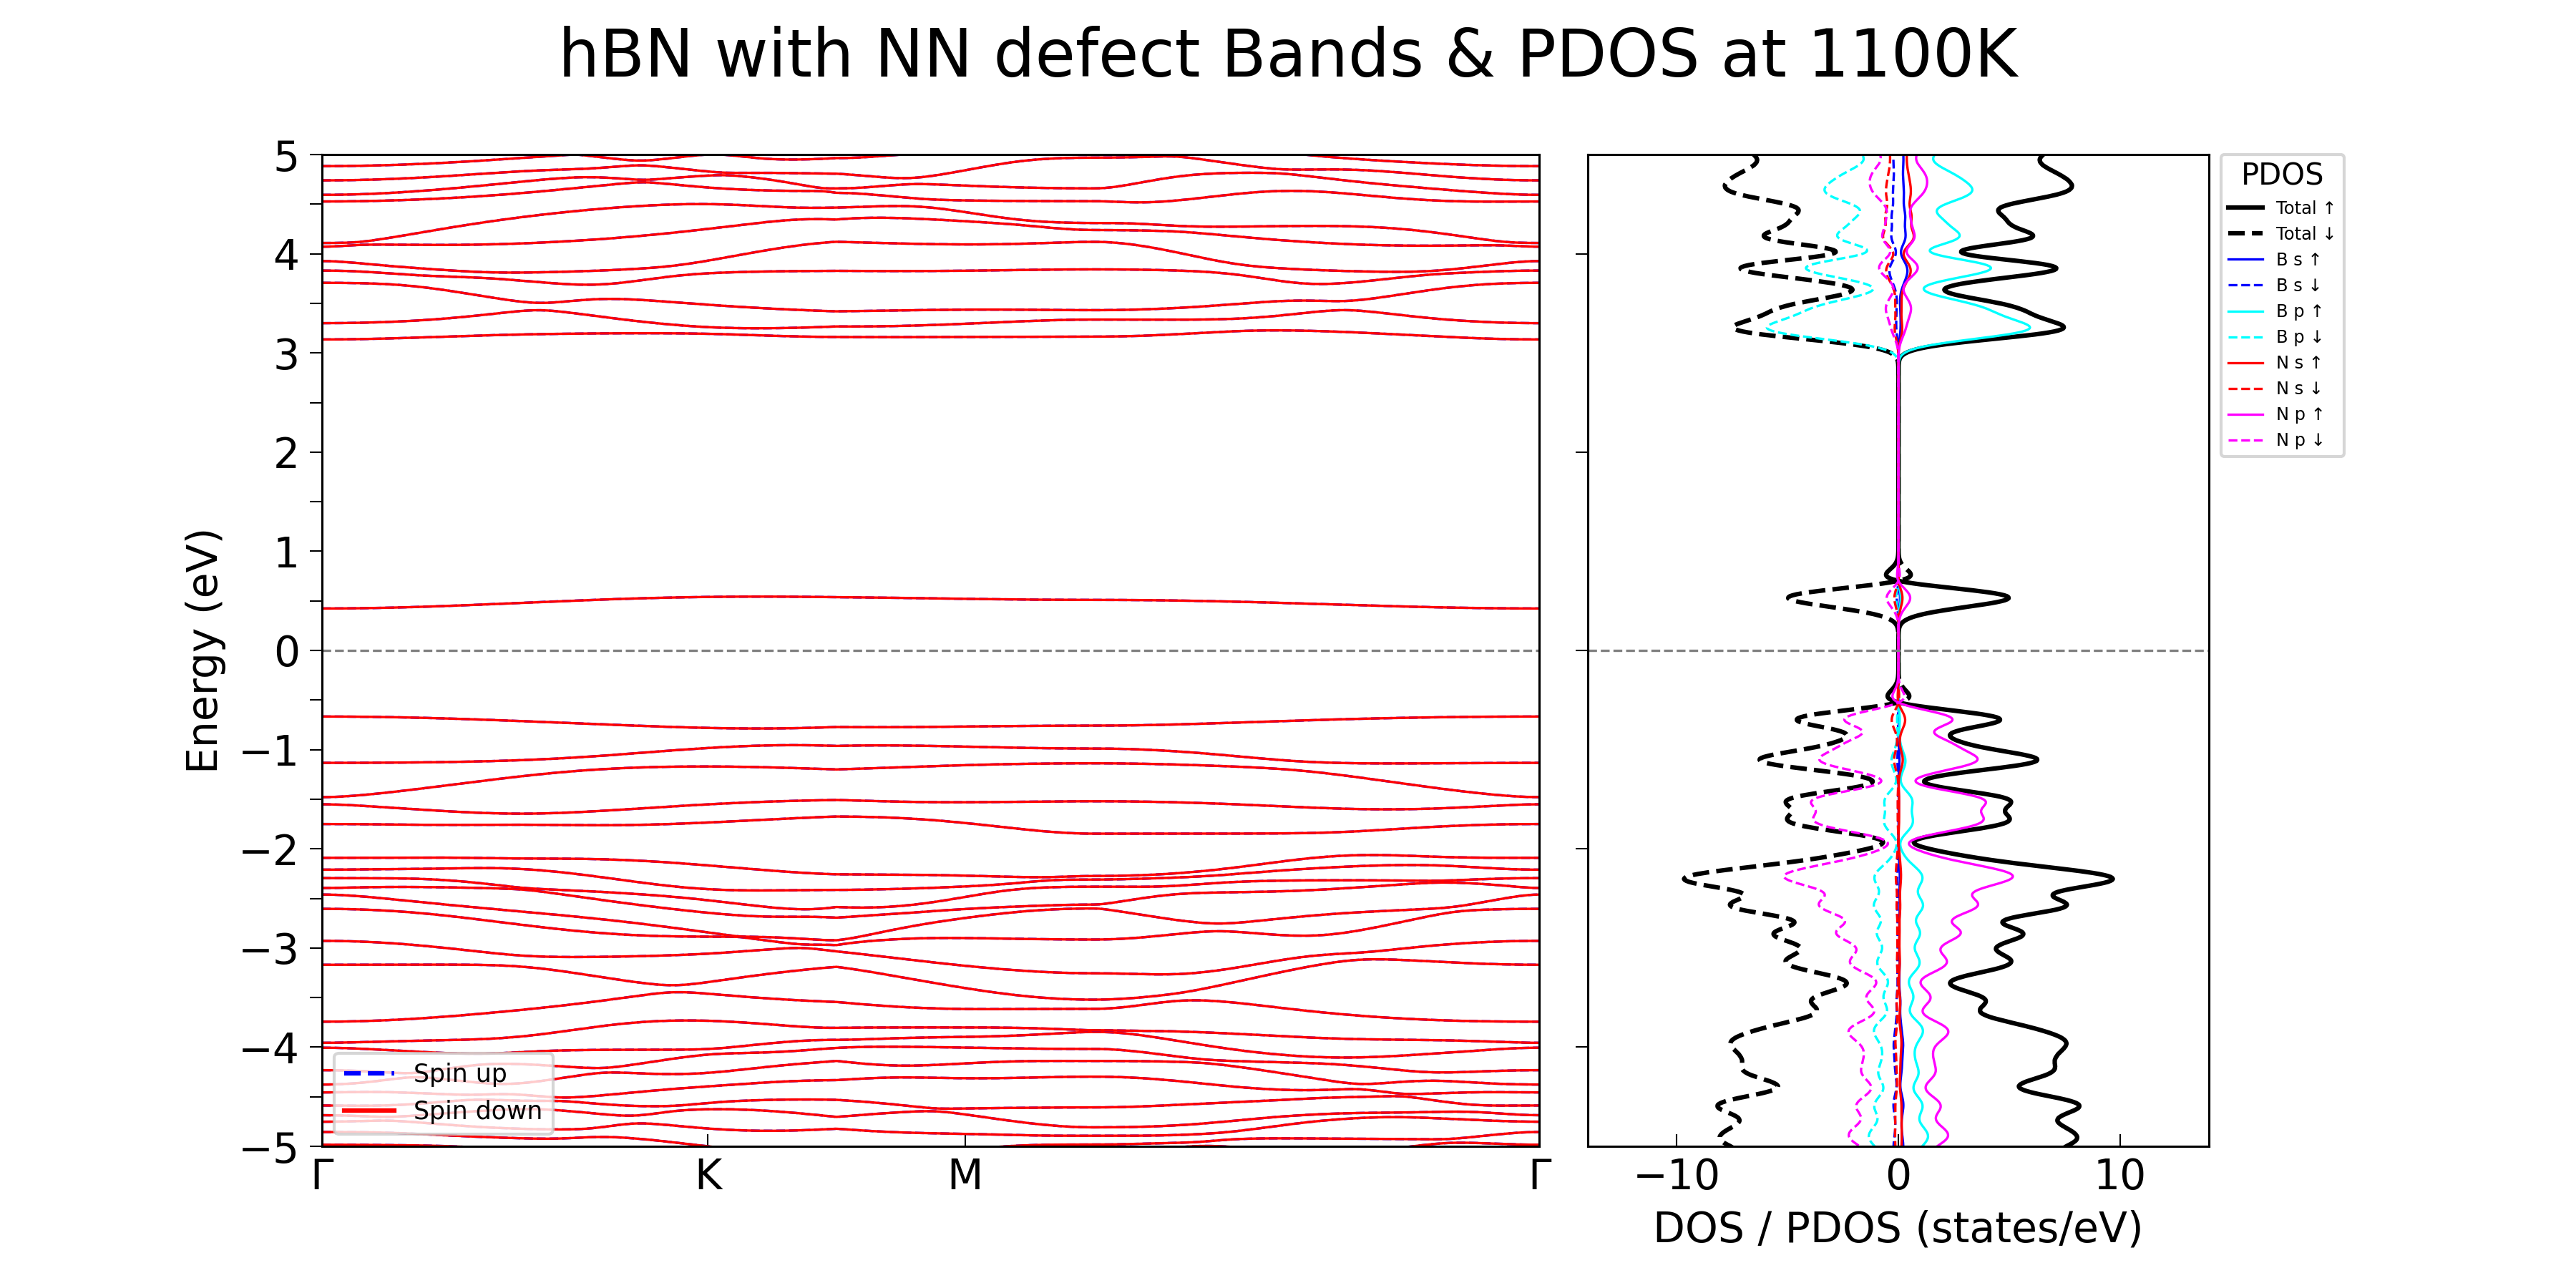
\includegraphics[width=0.95\textwidth]{gambar_hasil/simple_bands_pdos_NN_1100K.png}
    \caption{Struktur pita elektronik dan PDOS untuk monolayer hBN dengan cacat N\textsubscript{B} pada 1100 K. Celah pita efektif melebar menjadi $1.089$ eV.}
    \label{fig:hbn_NN_1100K}
\end{figure}
\begin{figure}[htbp!] % PERUBAHAN: Ukuran gambar diperbesar
    \centering
    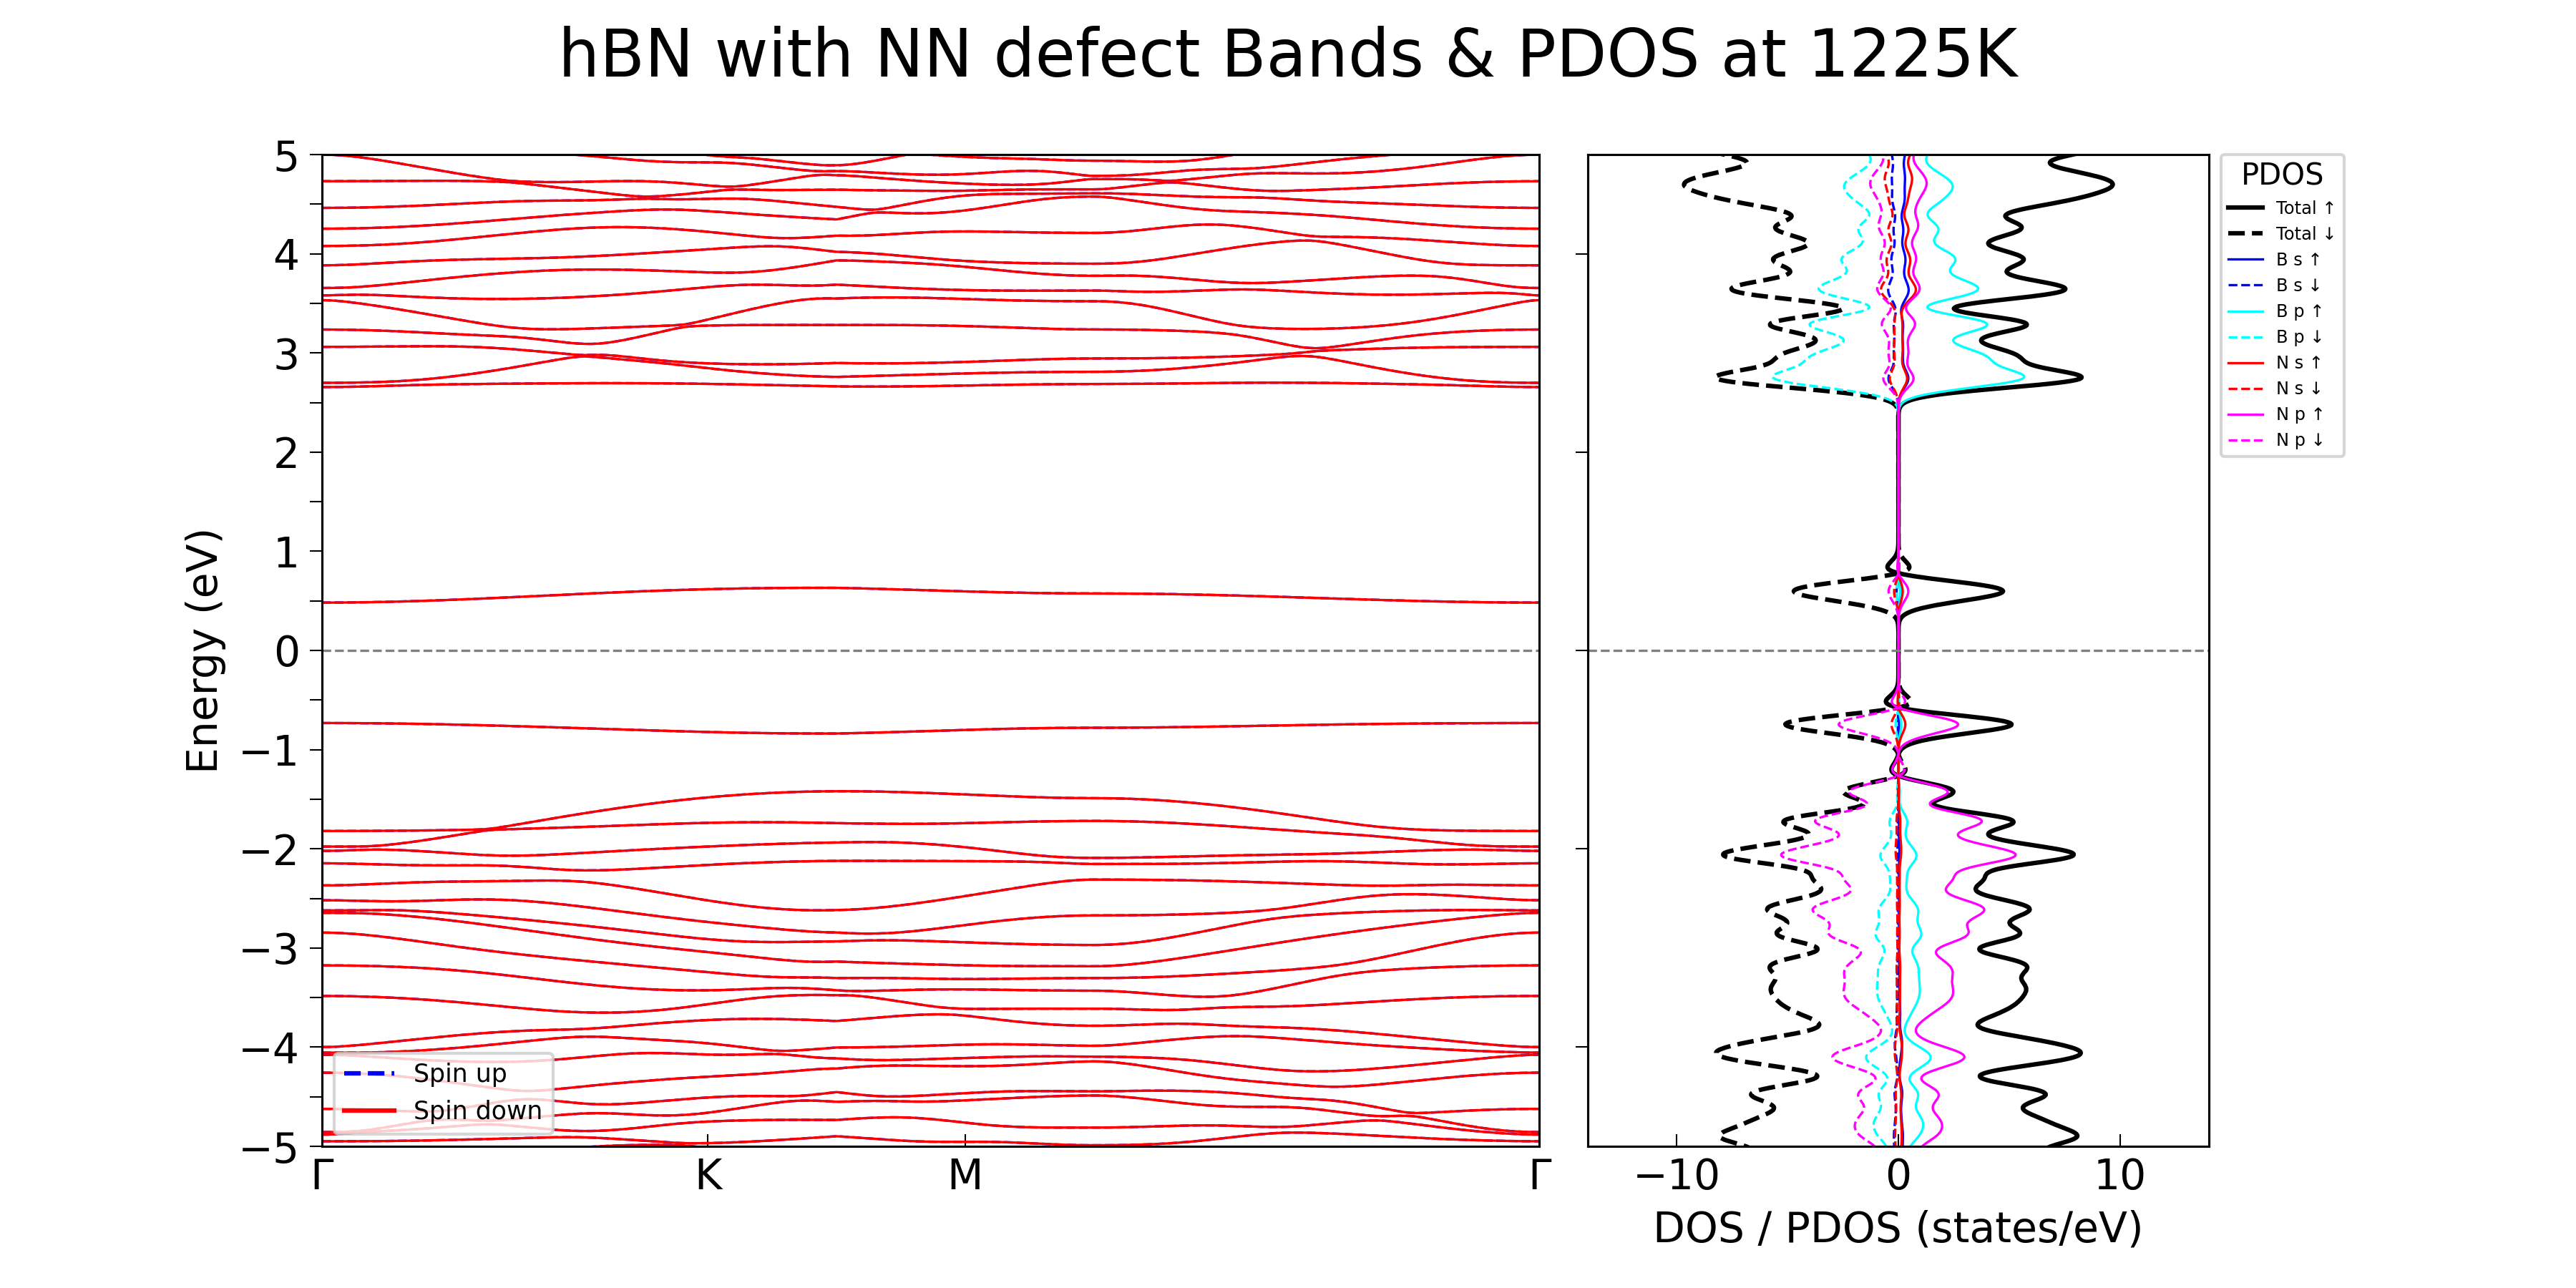
\includegraphics[width=0.95\textwidth]{gambar_hasil/simple_bands_pdos_NN_1225K.png}
    \caption{Struktur pita elektronik dan PDOS untuk monolayer hBN dengan cacat N\textsubscript{B} pada 1225 K. Celah pita terus melebar menjadi $1.214$ eV.}
    \label{fig:hbn_NN_1225K}
\end{figure}

Tren yang paling menonjol, seperti yang dirangkum dalam Tabel \ref{tab:hbn_defek_nb} dan diilustrasikan dari Gambar \ref{fig:hbn_NN_800K} hingga \ref{fig:hbn_NN_1225K}, adalah ketergantungan temperatur yang anomali dari celah pita.
Berlawanan dengan hBN murni, celah pita pada sistem dengan cacat N\textsubscript{B} justru \emph{meningkat} dengan kenaikan temperatur, dari $0.694$ eV pada 800 K menjadi $1.214$ eV pada 1225 K. Perilaku \emph{blueshift} anomali ini menunjukkan adanya mekanisme fisika yang berbeda secara fundamental.
Fenomena ini dapat dijelaskan oleh kopling elektron-fonon yang terlokalisasi. Celah pita efektif sekarang ditentukan oleh pemisahan energi antara keadaan cacat terisi dan tak terisi.
Keadaan-keadaan ini, karena sifatnya yang terlokalisasi di sekitar situs N\textsubscript{B}, sangat sensitif terhadap distorsi struktural lokal.
Vibrasi kisi (fonon) yang diaktifkan oleh suhu tinggi menyebabkan perubahan dinamis pada panjang ikatan dan sudut di sekitar cacat.
Untuk cacat N\textsubscript{B}, konfigurasi atomik yang terdistorsi oleh fonon ini secara kebetulan menghasilkan pemisahan energi yang lebih besar antara tingkat-tingkat cacat.
Dengan kata lain, fonon tidak lagi hanya menyebabkan "pencorengan" potensial global, tetapi secara aktif "memahat" lanskap energi lokal di sekitar cacat dengan cara yang memperlebar celah pitanya.
Sistem ini tetap non-magnetik di seluruh rentang temperatur yang diselidiki.

\subsubsection{Analisis Visual Kerapatan Muatan dan Spin untuk Cacat N\textsubscript{B}}
\label{subsec:hbn_NN_density_analysis}
Visualisasi distribusi elektron untuk sistem dengan cacat N\textsubscript{B} (Gambar \ref{fig:hbn_NN_density}) memberikan pemahaman yang lebih dalam tentang asal-usul perilaku elektroniknya yang unik.
\begin{figure}[htbp!] % PERUBAHAN: Ukuran gambar diperbesar
  \centering
  \begin{subfigure}[b]{0.49\textwidth}
    \centering
    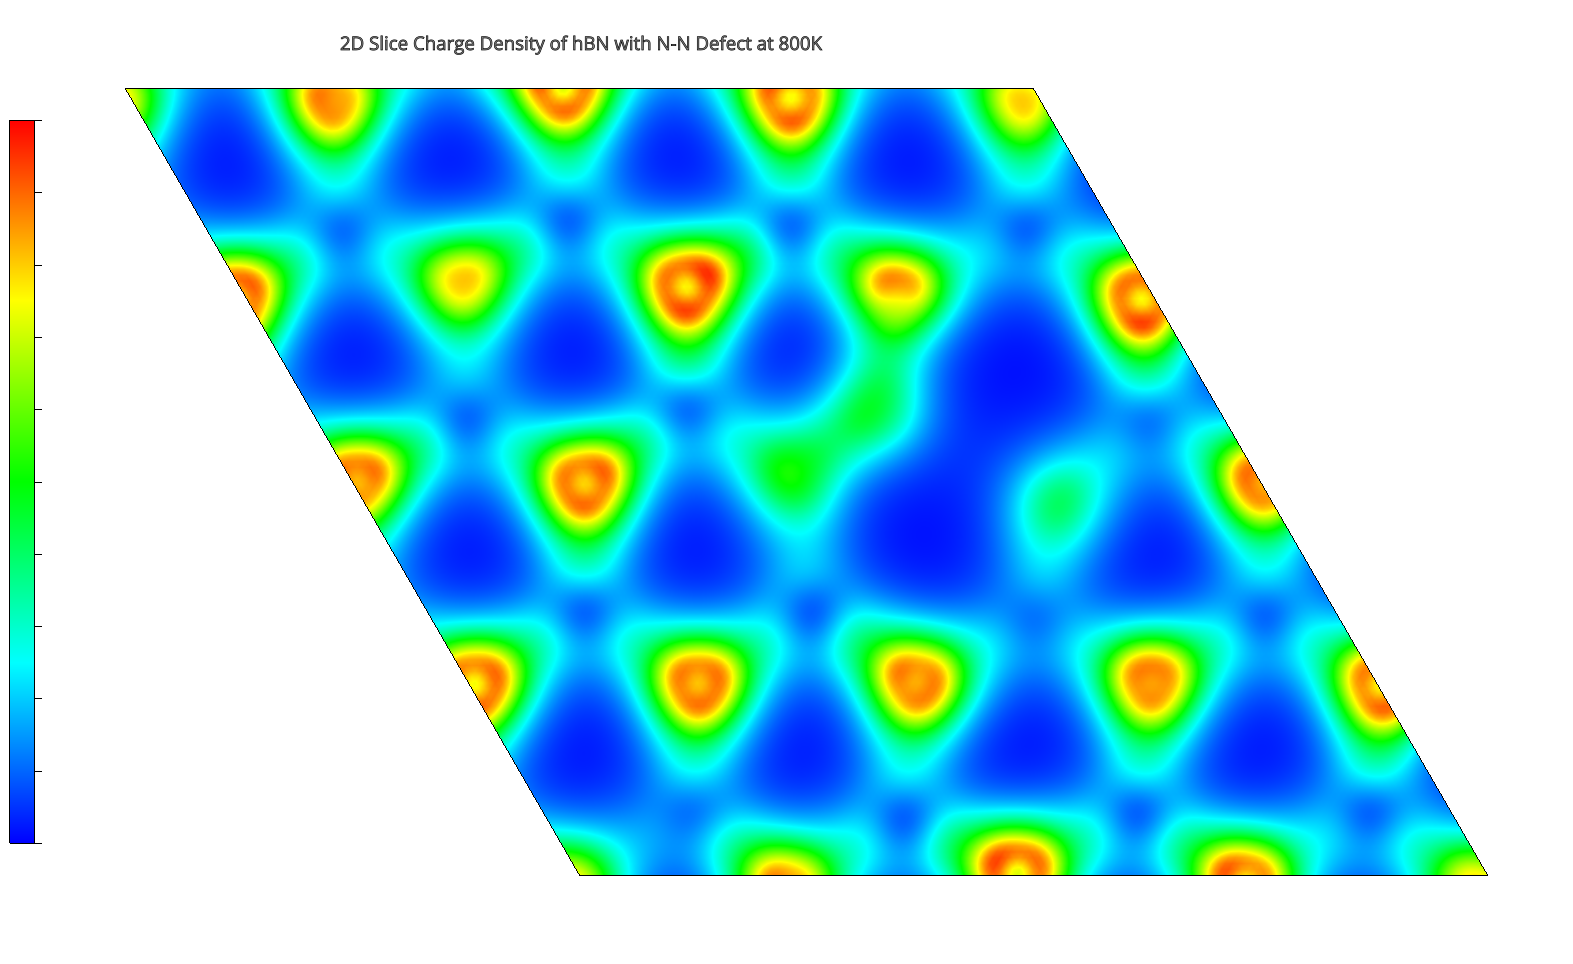
\includegraphics[width=\linewidth]{hBN_rho_NN_800K.png}
    \caption{Kerapatan Muatan, 800 K}
    \label{subfig:rho_nn_800k}
  \end{subfigure}\hfill
  \begin{subfigure}[b]{0.49\textwidth}
    \centering
    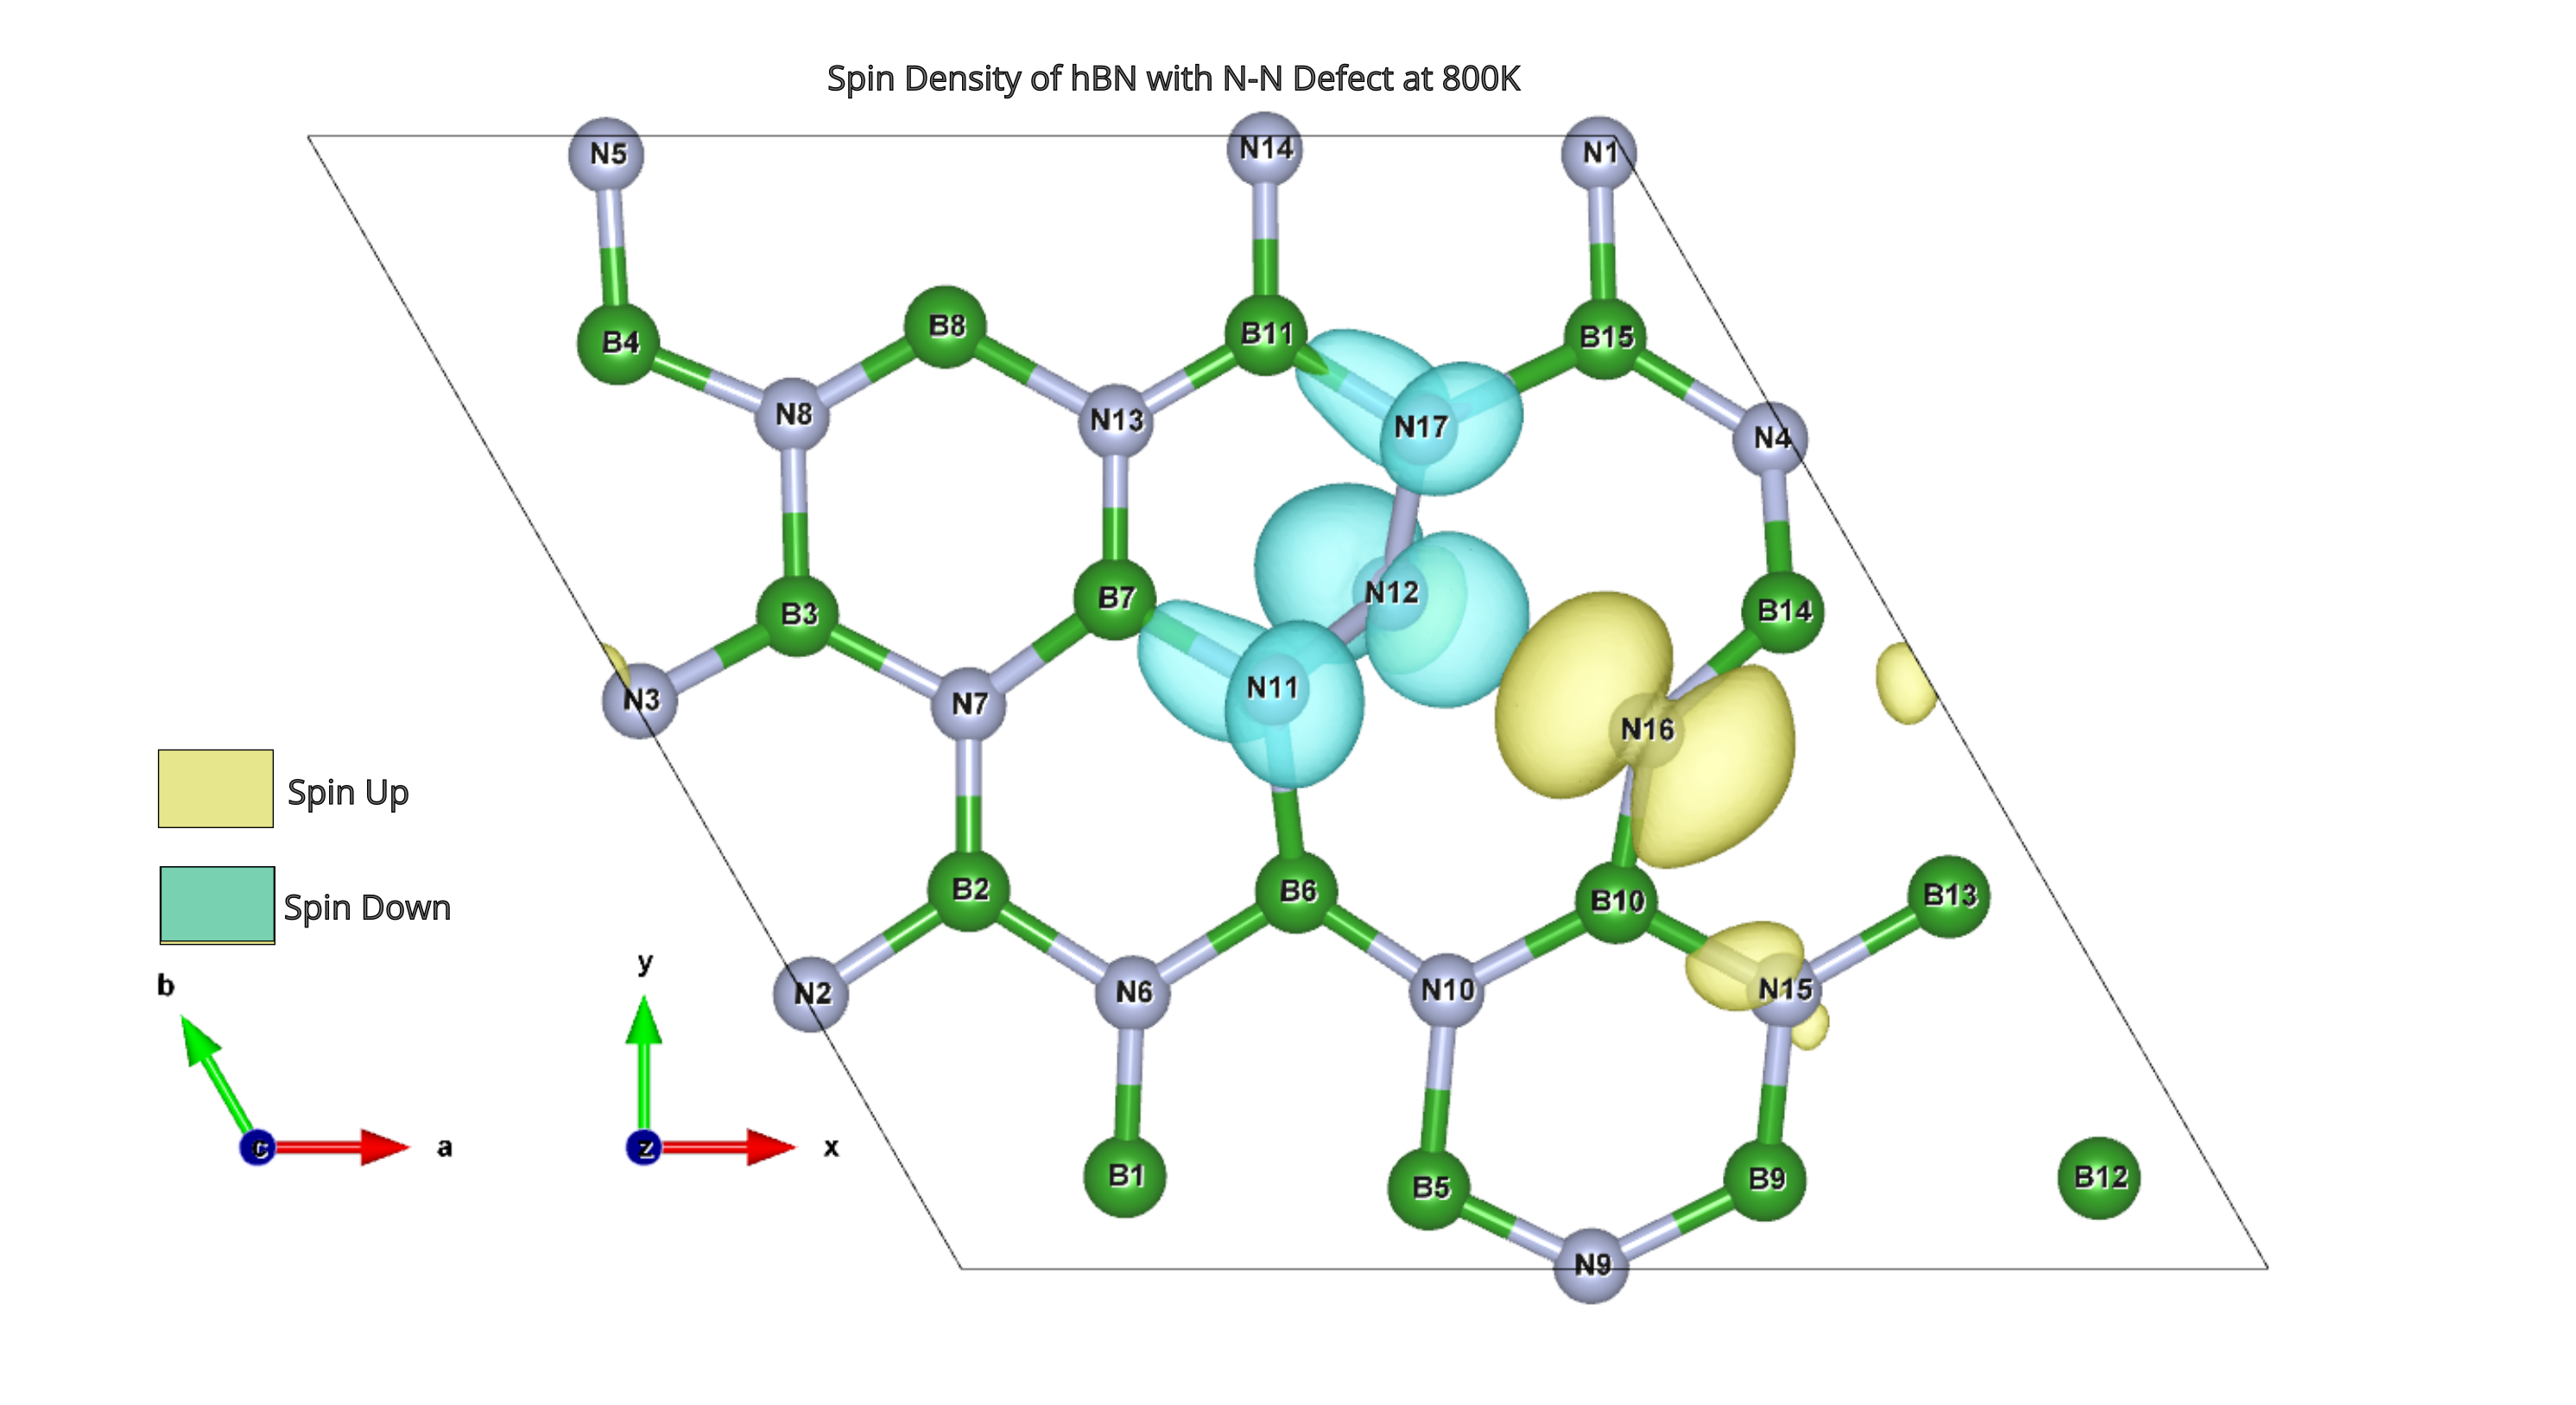
\includegraphics[width=\linewidth]{hBN_spin_NN_800K.png}
    \caption{Kerapatan Spin, 800 K}
    \label{subfig:spin_nn_800k}
  \end{subfigure}
  \vspace{1em}

  \begin{subfigure}[b]{0.49\textwidth}
    \centering
    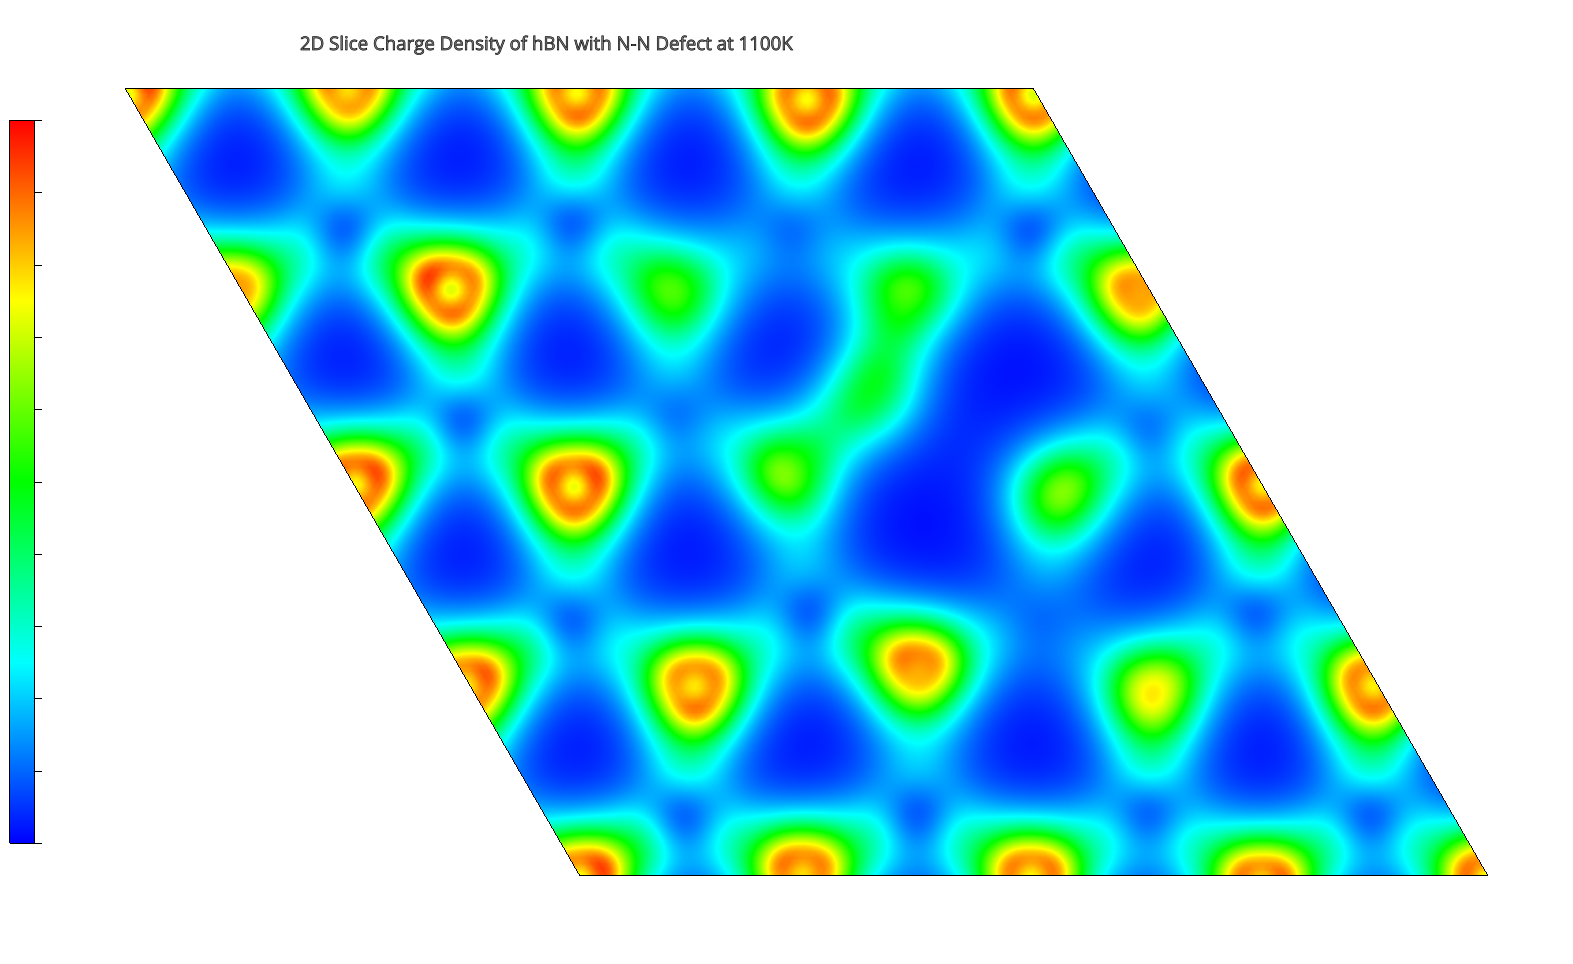
\includegraphics[width=\linewidth]{hBN_rho_NN_1100K.png}
    \caption{Kerapatan Muatan, 1100 K}
    \label{subfig:rho_nn_1100k}
  \end{subfigure}\hfill
  \begin{subfigure}[b]{0.49\textwidth}
    \centering
    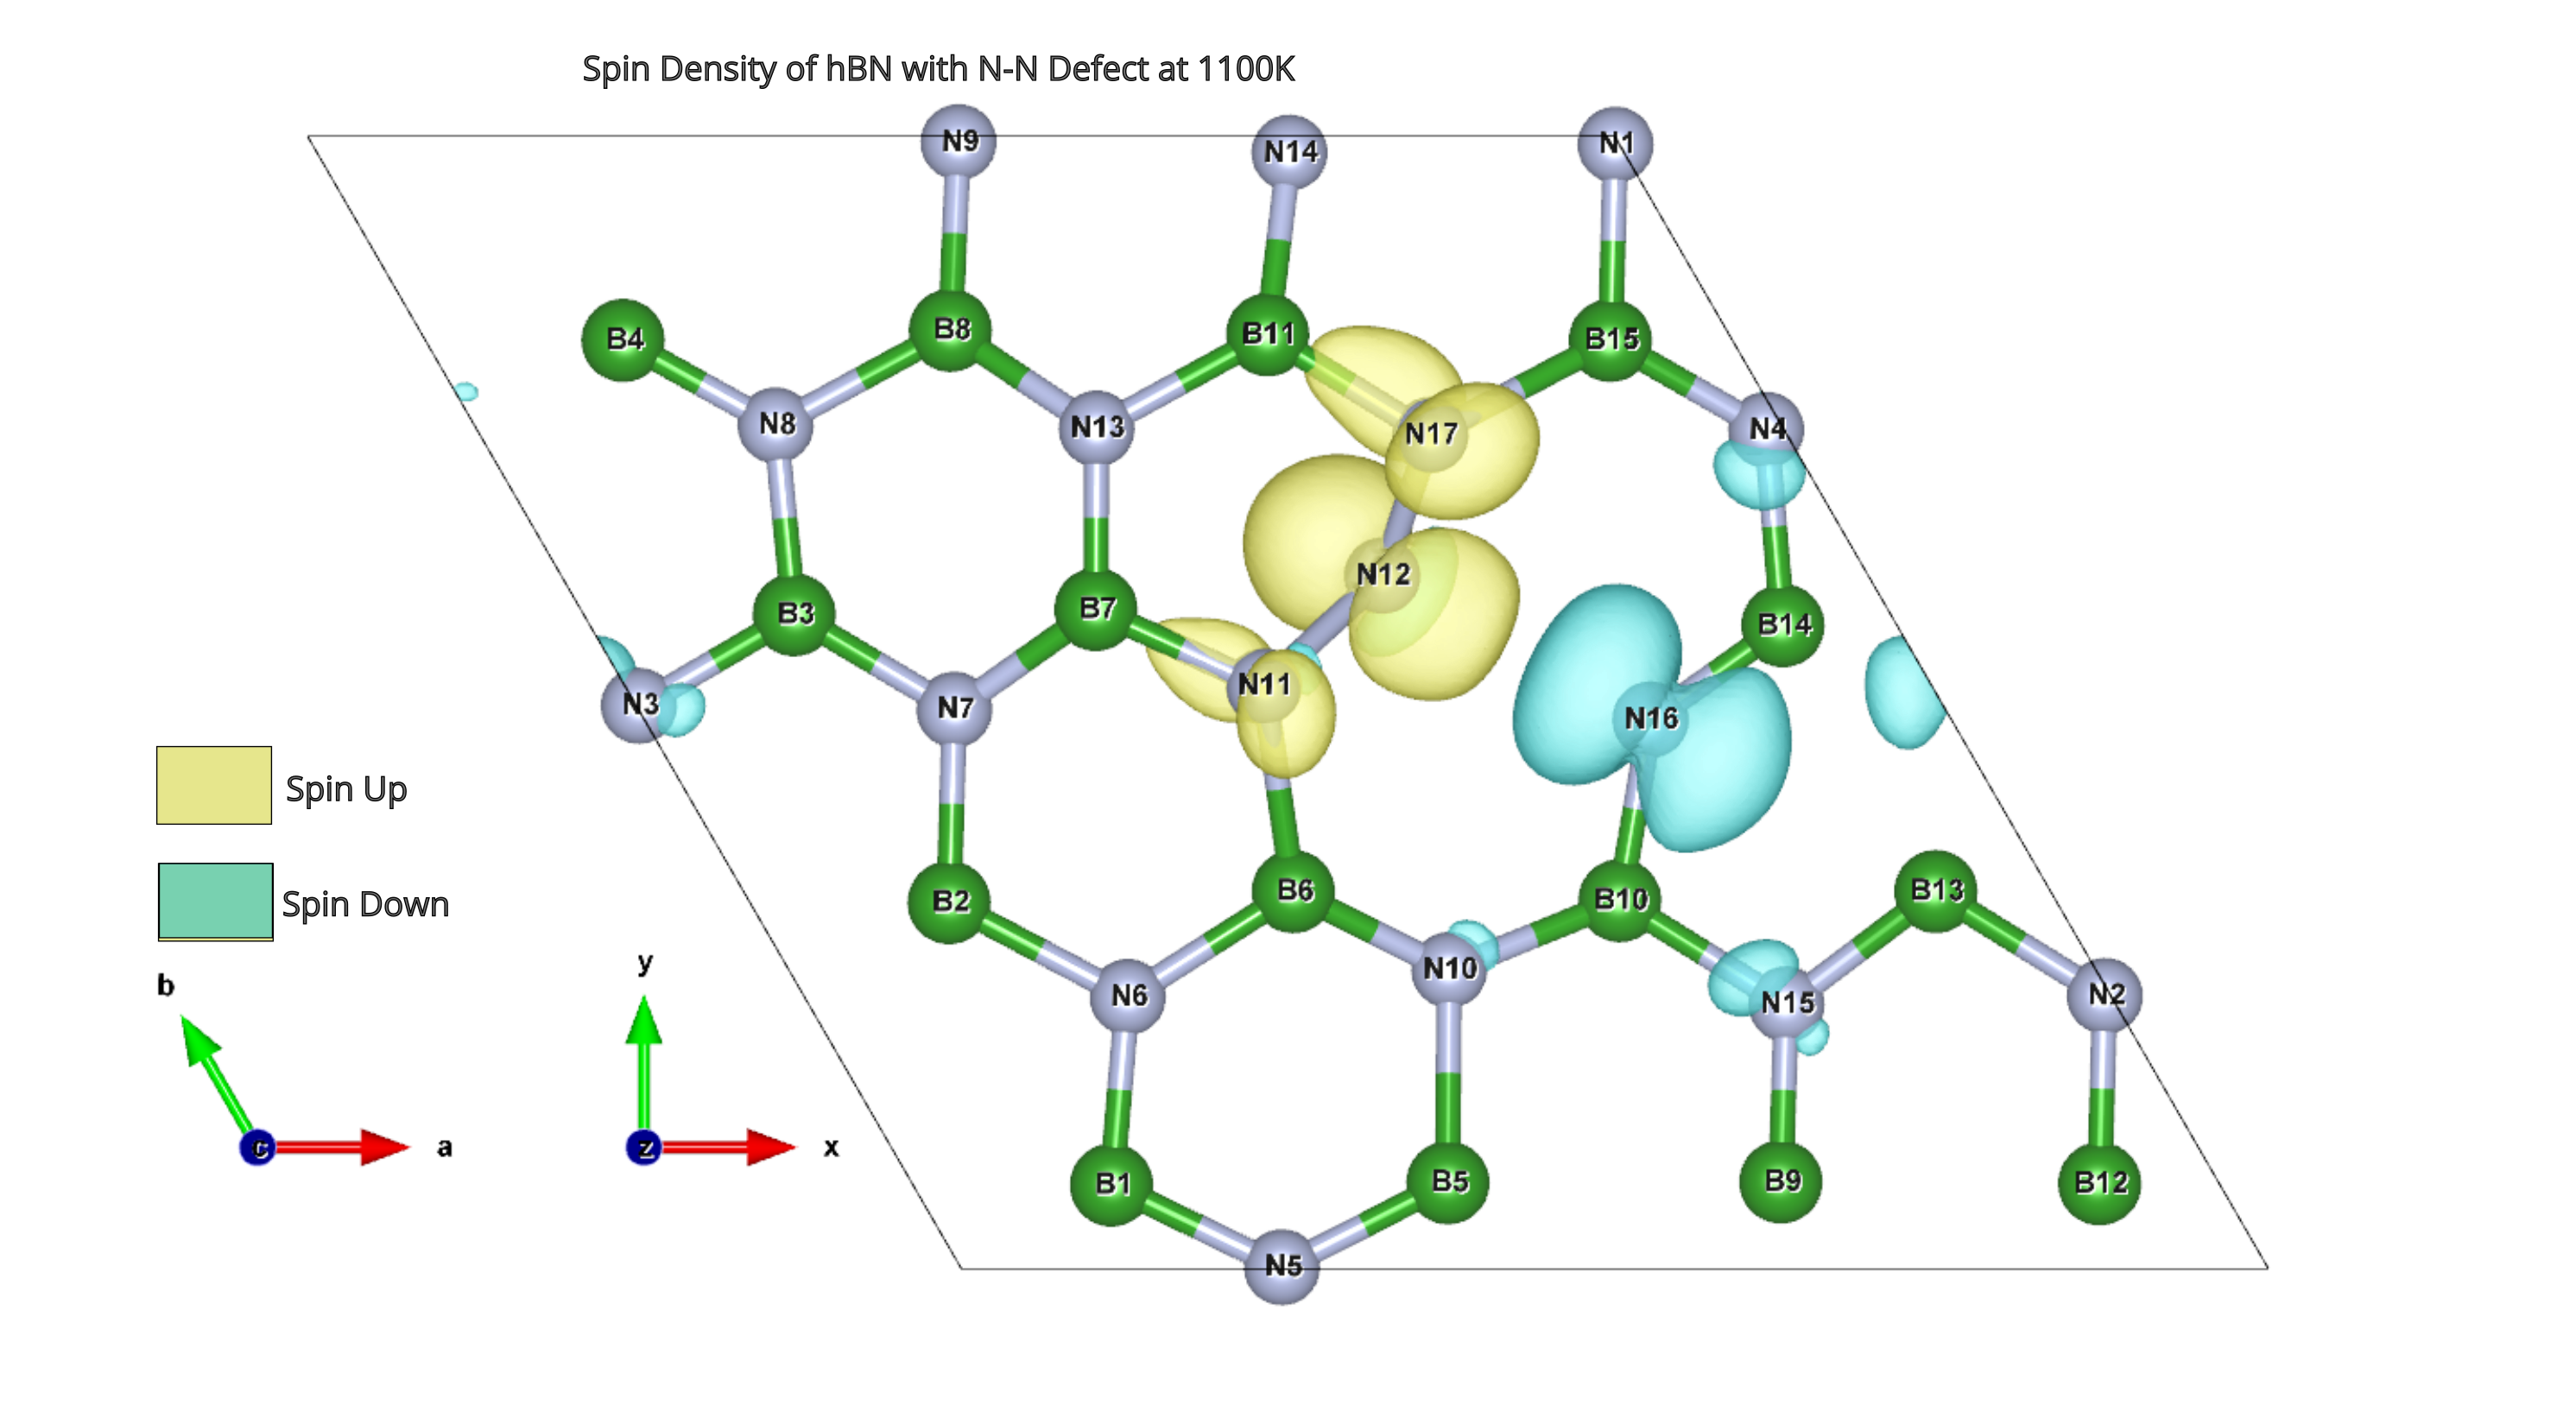
\includegraphics[width=\linewidth]{hBN_spin_NN_1100K.png}
    \caption{Kerapatan Spin, 1100 K}
    \label{subfig:spin_nn_1100k}
  \end{subfigure}
  \vspace{1em}

  \begin{subfigure}[b]{0.49\textwidth}
    \centering
    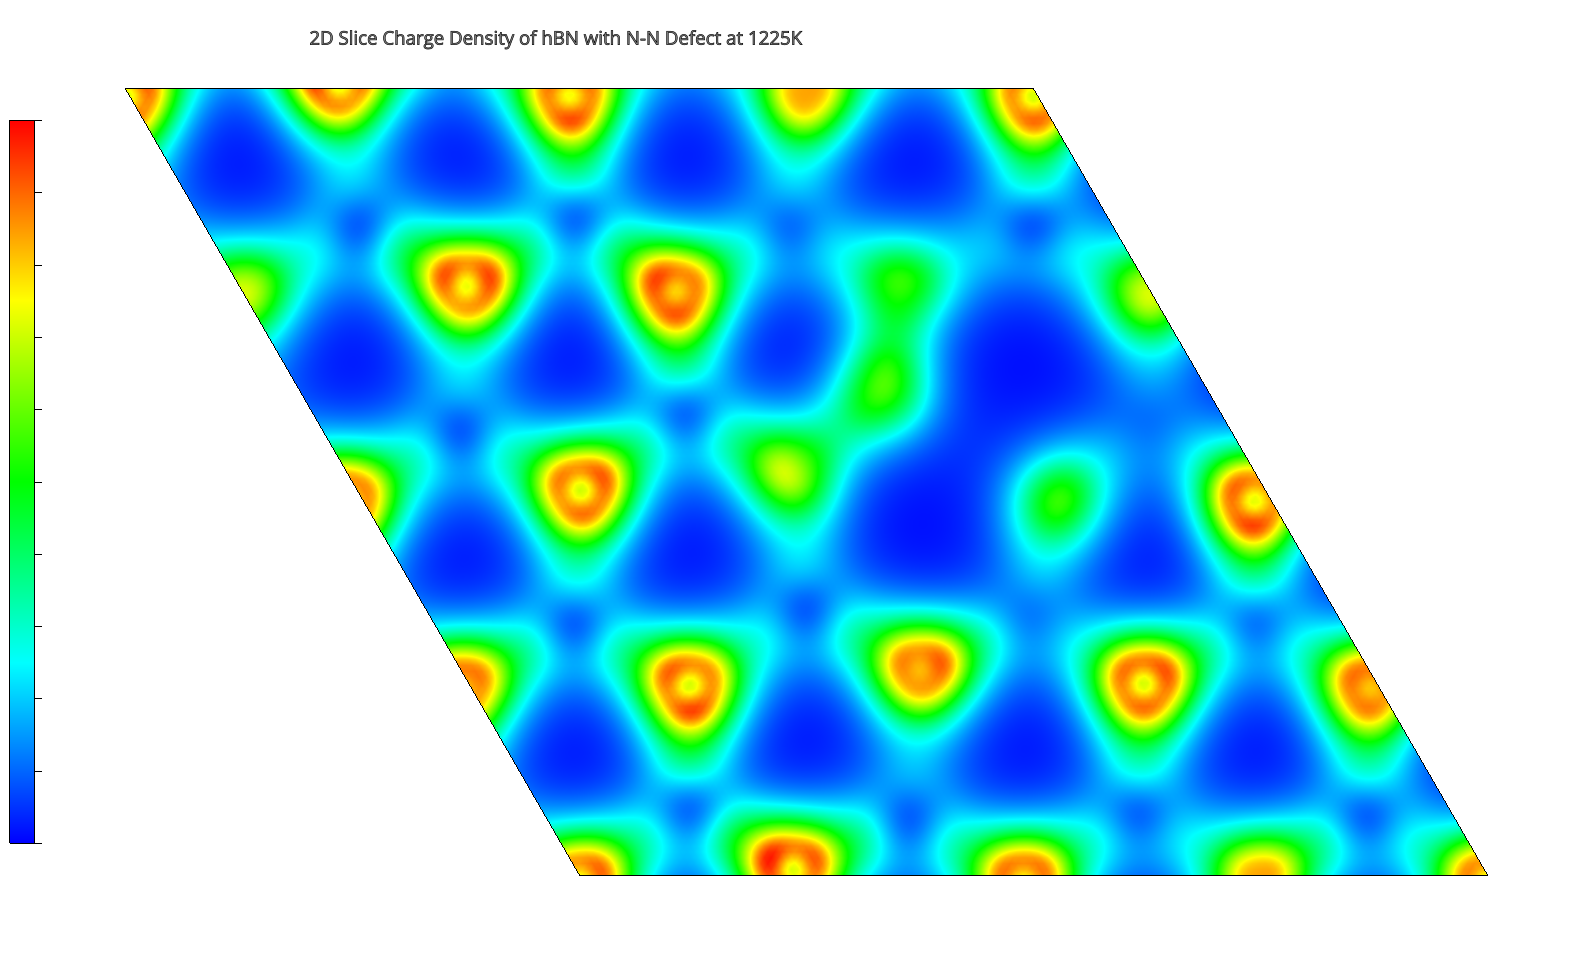
\includegraphics[width=\linewidth]{hBN_rho_NN_1225K.png}
    \caption{Kerapatan Muatan, 1225 K}
    \label{subfig:rho_nn_1225k}
  \end{subfigure}\hfill
  \begin{subfigure}[b]{0.49\textwidth}
    \centering
    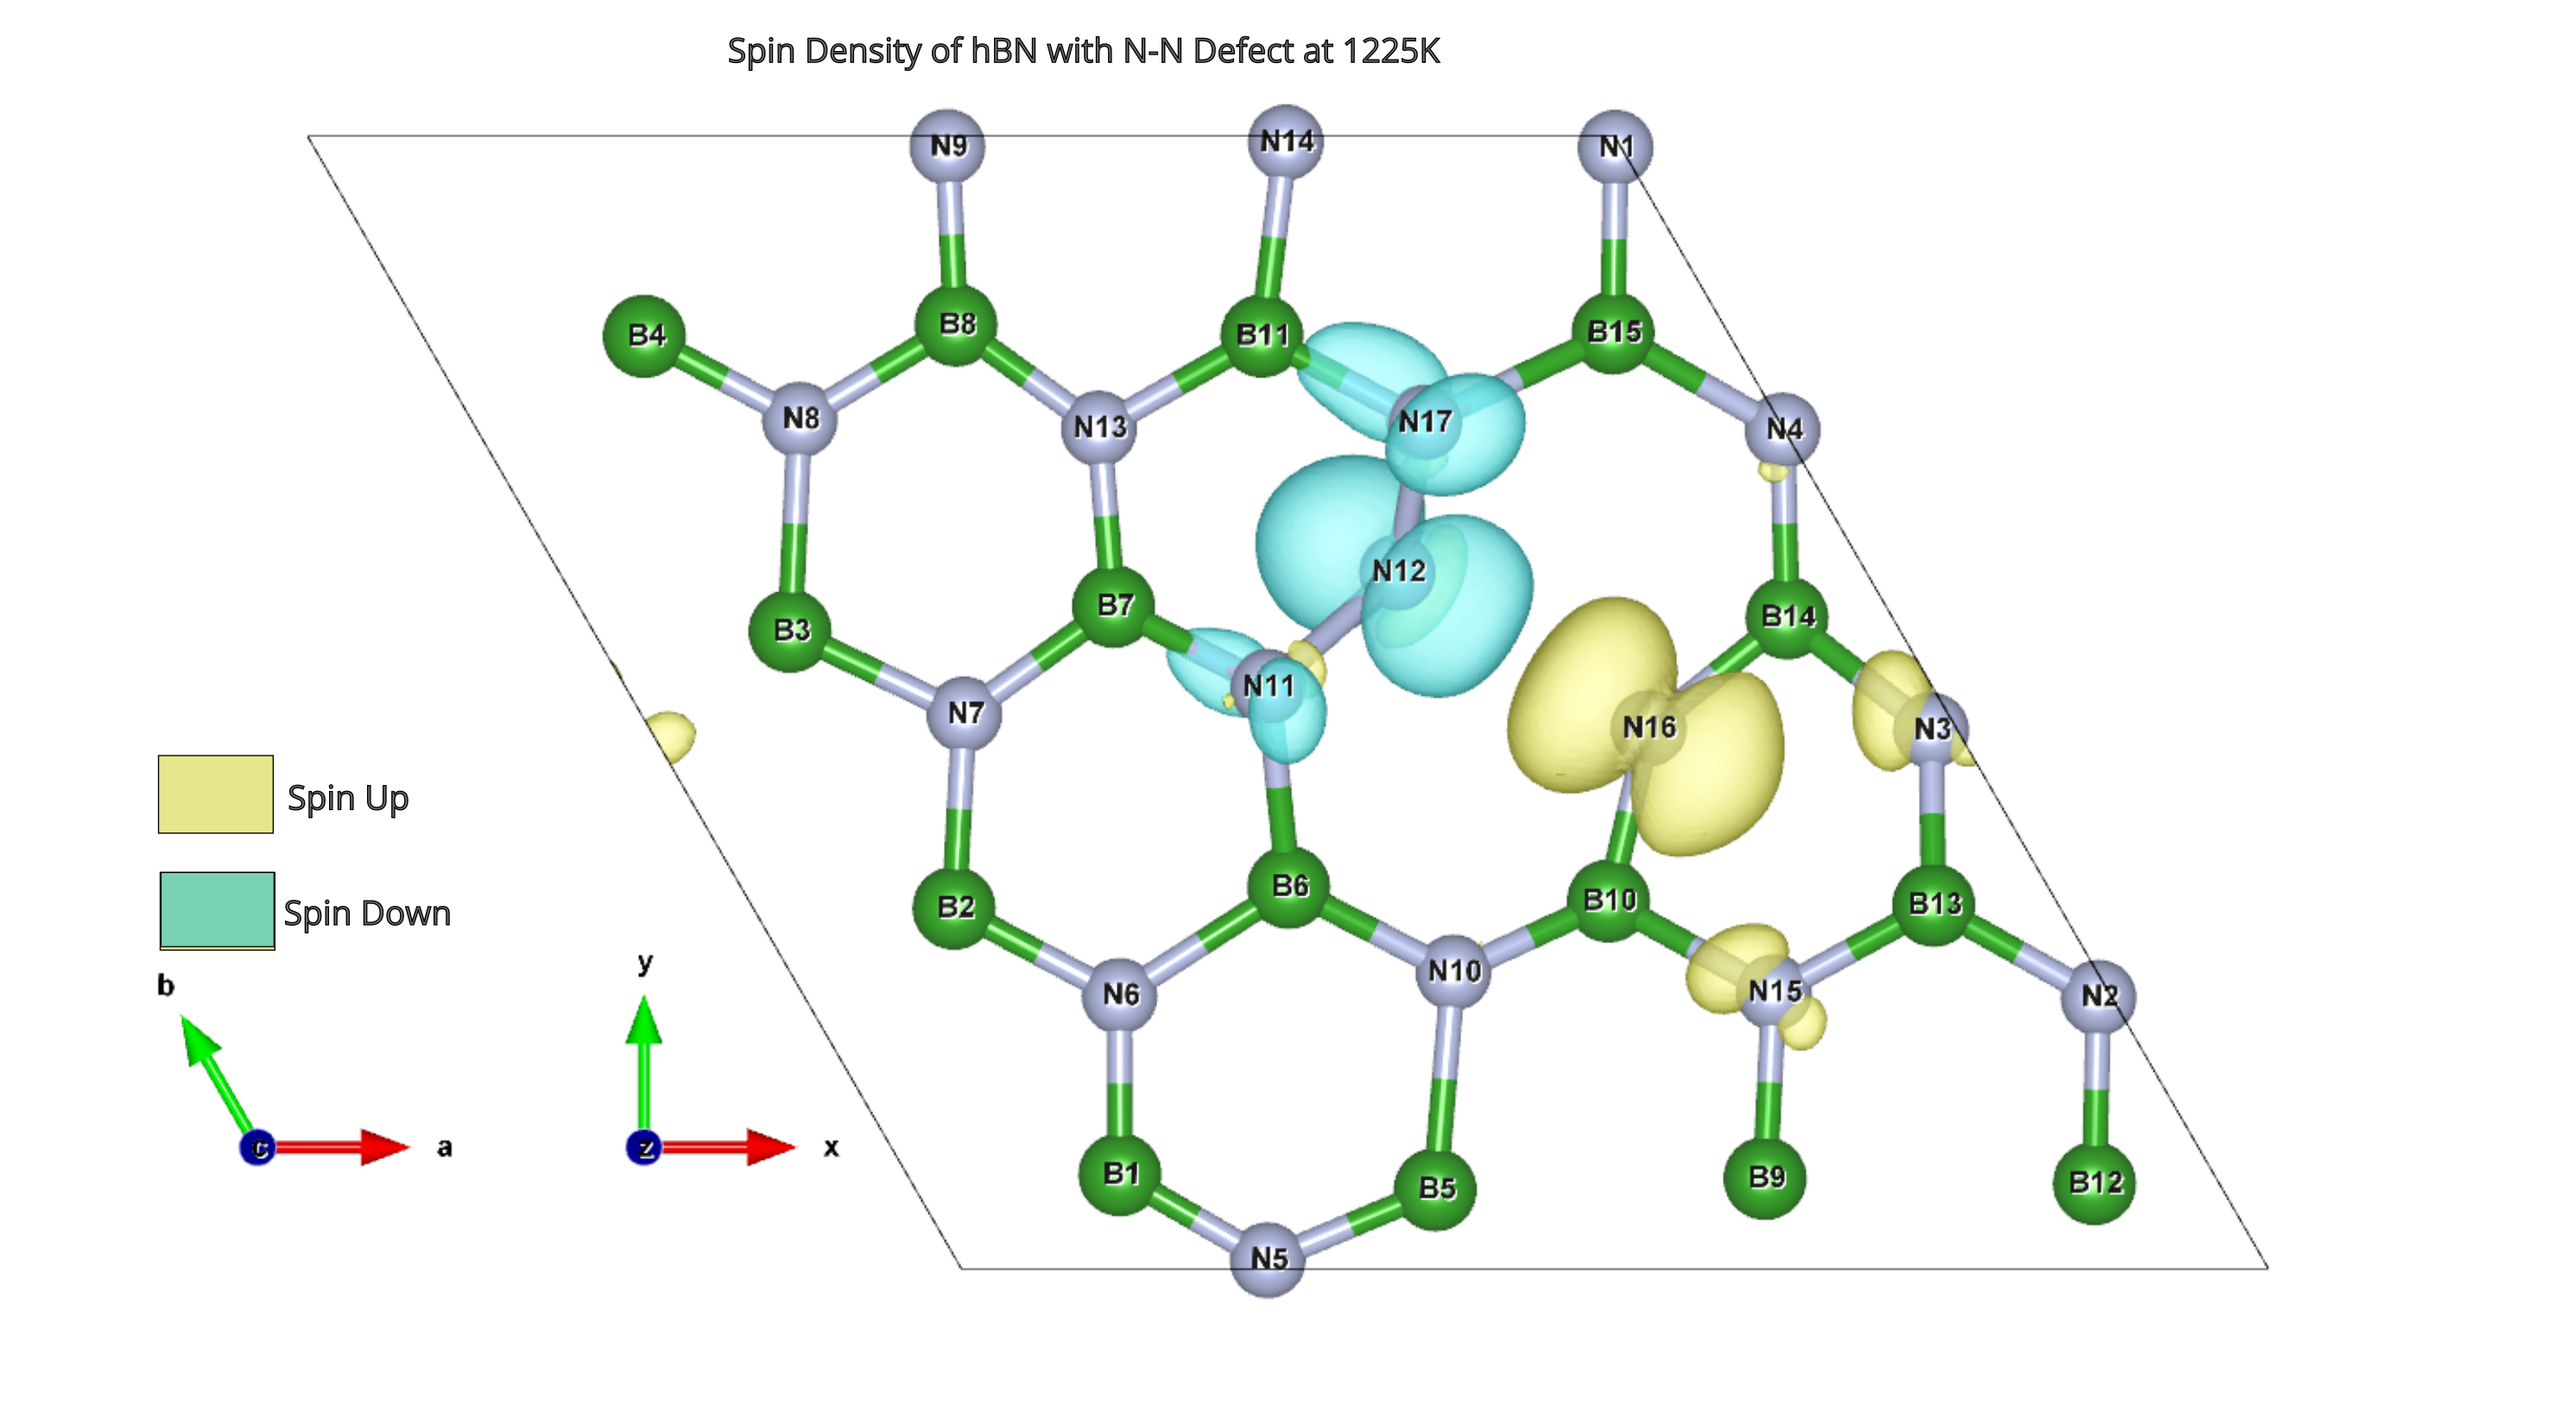
\includegraphics[width=\linewidth]{hBN_spin_NN_1225K.png}
    \caption{Kerapatan Spin, 1225 K}
    \label{subfig:spin_nn_1225k}
  \end{subfigure}
  \caption{Visualisasi 2D dari kerapatan muatan total (kiri) dan kerapatan spin (kanan) untuk monolayer hBN dengan cacat N\textsubscript{B} pada 800 K, 1100 K, dan 1225 K. Kehadiran cacat menciptakan perturbasi lokal yang jelas pada kerapatan muatan. Warna merah pada kerapatan muatan menunjukkan akumulasi elektron, sedangkan warna biru menunjukkan deplesi. Untuk kerapatan spin, warna biru menunjukkan spin down dan warna kuning menunjukan spin up.}
  \label{fig:hbn_NN_density}
\end{figure}

Plot kerapatan muatan (Gambar \ref{fig:hbn_NN_density}a, c, e) dengan jelas menunjukkan bagaimana cacat N\textsubscript{B} mematahkan simetri translasi dari kisi hBN yang sempurna.
Terlihat adanya perturbasi yang sangat terlokalisasi pada distribusi muatan, yang berpusat di sekitar lokasi cacat.
Secara spesifik, pembentukan ikatan N-N antara atom nitrogen antisite dan tetangga nitrogennya menciptakan sebuah fitur elektronik yang berbeda dari ikatan B-N di sekitarnya.
Gangguan lokal inilah yang menjadi akar penyebab munculnya tingkat-tingkat energi cacat yang terlokalisasi di dalam celah pita, seperti yang diamati pada plot struktur pita (misalnya, Gambar \ref{fig:hbn_NN_800K}).
Lingkungan elektronik yang terbatas dan terisolasi ini sangat rentan terhadap perubahan geometri lokal, yang menjelaskan mengapa vibrasi termal (fonon) memiliki dampak yang begitu kuat dan spesifik (yaitu, \emph{blueshift}) pada tingkat energi cacat ini.
Serupa dengan kasus murni, plot kerapatan spin (Gambar \ref{fig:hbn_NN_density}b, d, f) menunjukkan polarisasi spin nol di seluruh sistem dan pada semua temperatur.
Meskipun Tabel \ref{tab:hbn_defek_nb} menunjukkan nilai magnetisasi absolut yang sangat kecil dan non-nol ($0.010 \mu_B$) pada 1225 K, visualisasi ini mengonfirmasi bahwa nilai tersebut adalah derau komputasi (\emph{computational noise}) dan bukan merupakan indikasi tatanan magnetik yang sebenarnya.
Ini adalah poin pembeda yang penting jika dibandingkan dengan cacat B\textsubscript{N}.
Bukti visual ini menunjukkan bahwa meskipun cacat N\textsubscript{B} secara signifikan mengubah struktur elektronik orbital, ia menciptakan keadaan yang secara elektronik "terpenuhi" atau "jenuh" yang tidak memiliki karakter elektron tak berpasangan yang diperlukan untuk memicu pemisahan spin (memenuhi kriteria Stoner).
Hal ini memperkuat kesimpulan bahwa fisika yang dominan dalam sistem N\textsubscript{B} diatur oleh interaksi muatan-fonon, bukan interaksi spin-fonon.

\subsection{Cacat B\textsubscript{N}: Induksi Magnetisme $d^0$ dan Kopling Spin-Fonon}
\label{subsec:hbn_defek_bn}
Cacat antisite B\textsubscript{N} menginduksi perubahan yang paling dramatis, yaitu kemunculan magnetisme yang bergantung pada temperatur.
Pada 800 K, sistem ini bersifat non-magnetik dengan celah pita $0.990$ eV (Gambar \ref{fig:hbn_BB_800K}).
Namun, seperti yang ditunjukkan pada Tabel \ref{tab:hbn_defek_bn}, transisi fasa magnetik terjadi pada temperatur yang lebih tinggi.
\begin{table}[htbp!] % STANDARISASI: Menggunakan [htbp!]
  \centering
  \caption{Sifat Elektronik dan Magnetik Monolayer hBN dengan Cacat Antisite B\textsubscript{N} sebagai Fungsi Temperatur.}
  \label{tab:hbn_defek_bn}
  % ANOTASI: \resizebox digunakan di sini sebagai solusi pragmatis untuk tabel
  % yang sangat lebar. Ini memastikan tabel pas di dalam lebar teks.
  % Namun, ini dapat menyebabkan ukuran font yang tidak konsisten dengan
  % teks lainnya. Untuk publikasi formal, alternatif seperti memformat ulang
  % tabel, menggunakan singkatan, atau menggunakan lingkungan 'sidewaystable'
  % (dari paket 'rotating') mungkin lebih disukai.
  \resizebox{\textwidth}{!}{%
  \begin{tabular}{lcccccccccc}
    \toprule
    Temperatur & VBM & CBM & $E_g$ Sistem & $E_F$ & Mag. Total & Mag. Abs. & Momen Orbital & Momen Orbital & Momen Orbital & Momen Orbital \\
    (K) & (eV) & (eV) & Total (eV) & (eV) & ($\mu_B$) & ($\mu_B$) & B-s ($\mu_B$) & B-p ($\mu_B$) & N-s ($\mu_B$) & N-p ($\mu_B$) \\
    \midrule
    800  & -0.633 & 0.357 & 0.990 & -0.249 & 0.000 & 0.000 & -0.000 & 0.000 & -0.000 & 0.000 \\
    1100 & -0.120 ($\downarrow$) & 0.301 ($\uparrow$)  & 0.421 & -0.410 & 0.150 & 0.230 &  0.003 & 0.010 & -0.000 & 0.001 \\
    1225 & -0.073 ($\uparrow$) & 0.243 ($\downarrow$)  & 0.316 & -0.622 & 1.850 & 2.320 &  0.057 & 0.009 & -0.022 & -0.002 \\
    \bottomrule
  \end{tabular}%
  }
\end{table}

\begin{figure}[htbp!] % PERUBAHAN: Ukuran gambar diperbesar
    \centering
    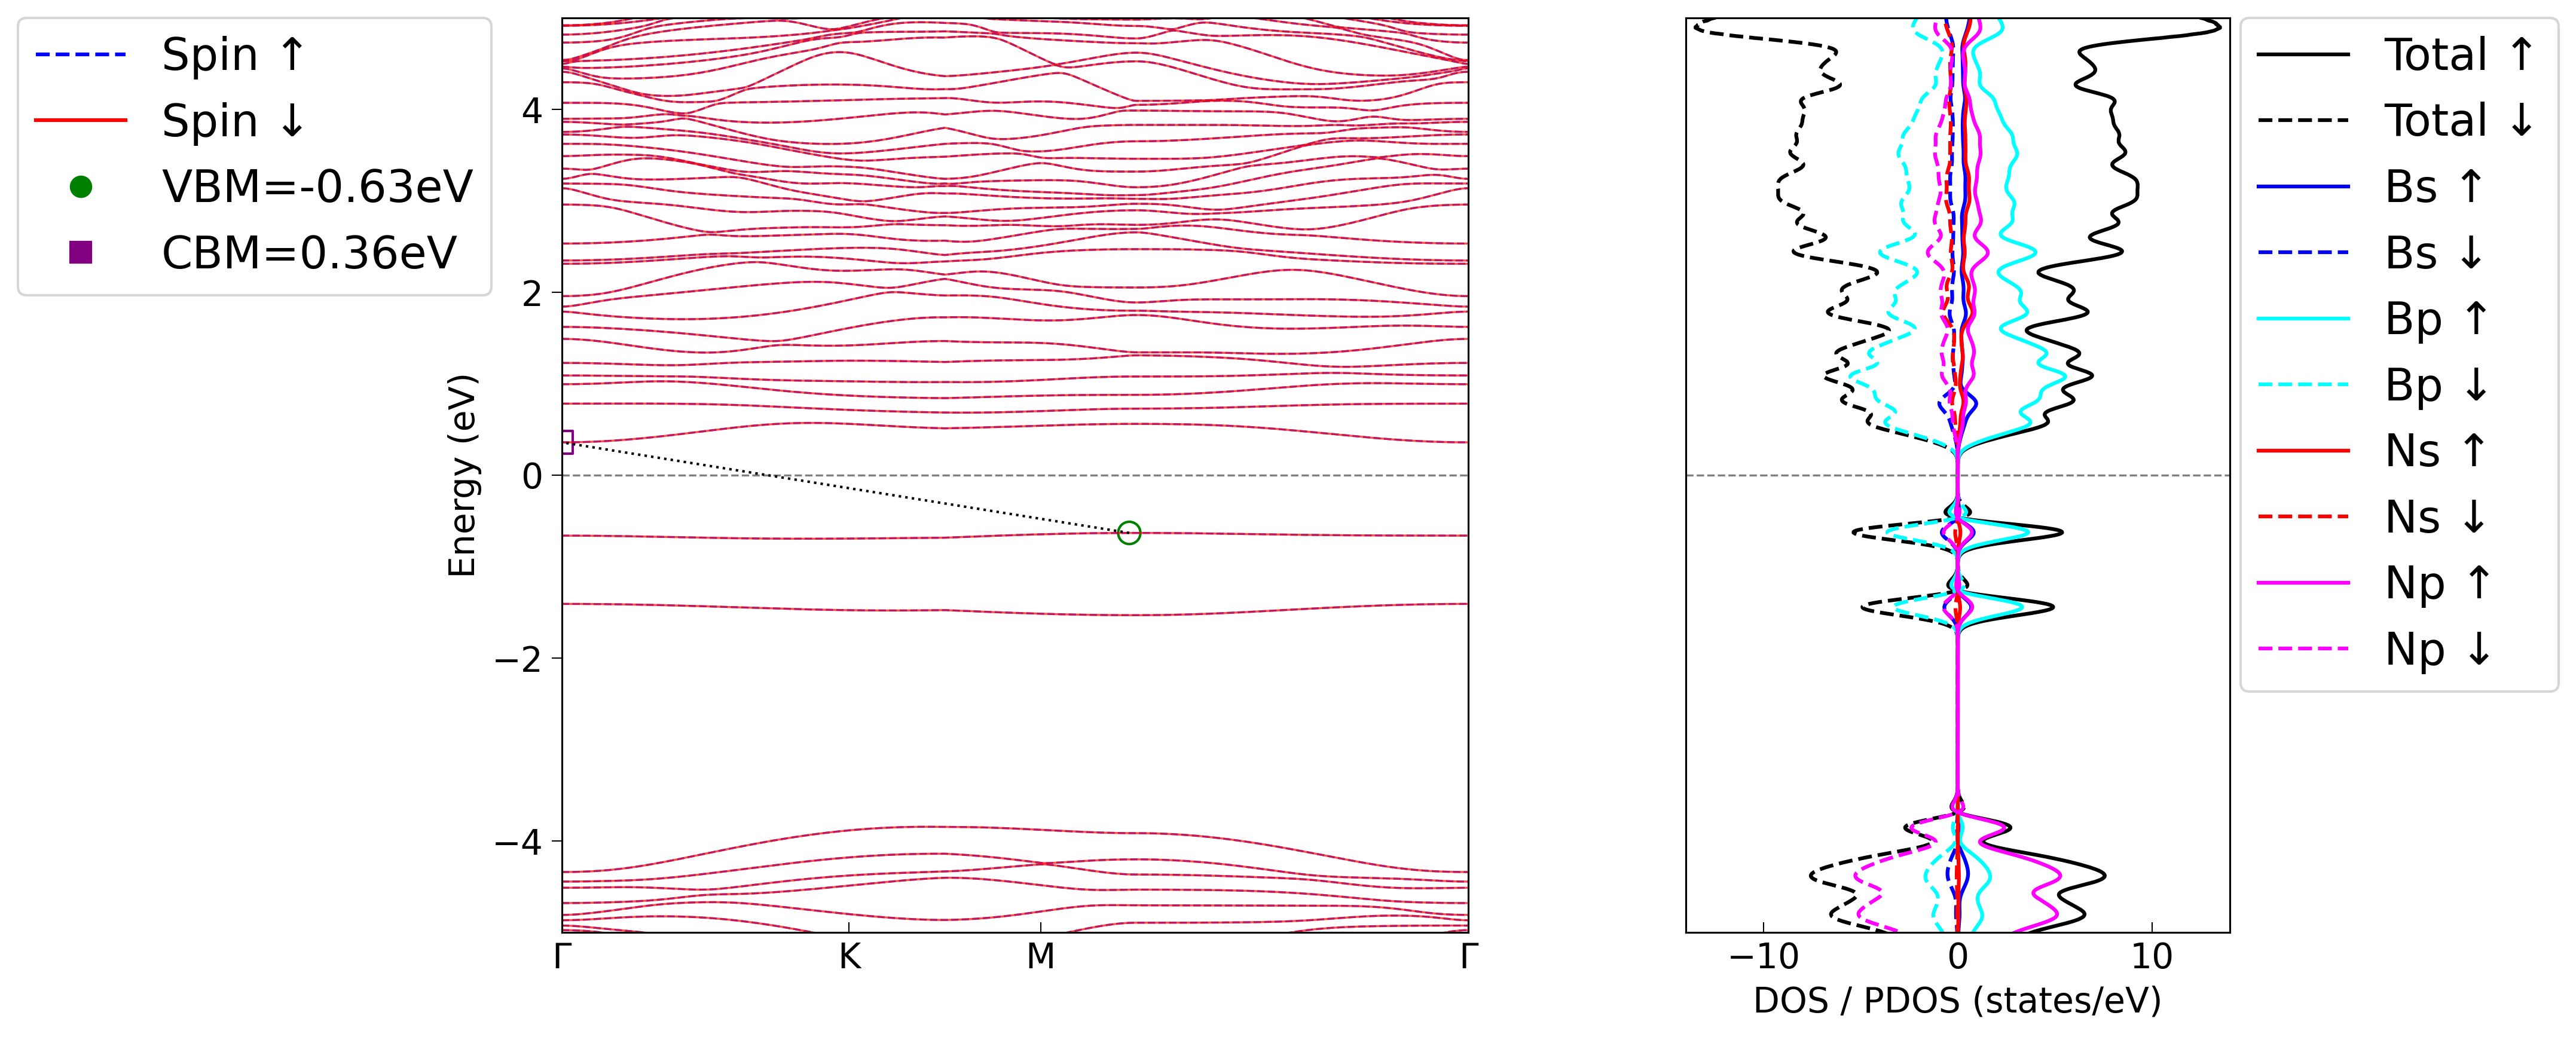
\includegraphics[width=0.95\textwidth]{gambar_hasil/simple_bands_pdos_BB_800K.png}
    \caption{Struktur pita elektronik dan PDOS untuk monolayer hBN dengan cacat B\textsubscript{N} pada 800 K. Sistem bersifat non-magnetik.}
    \label{fig:hbn_BB_800K}
\end{figure}
\begin{figure}[htbp!] % PERUBAHAN: Ukuran gambar diperbesar
    \centering
    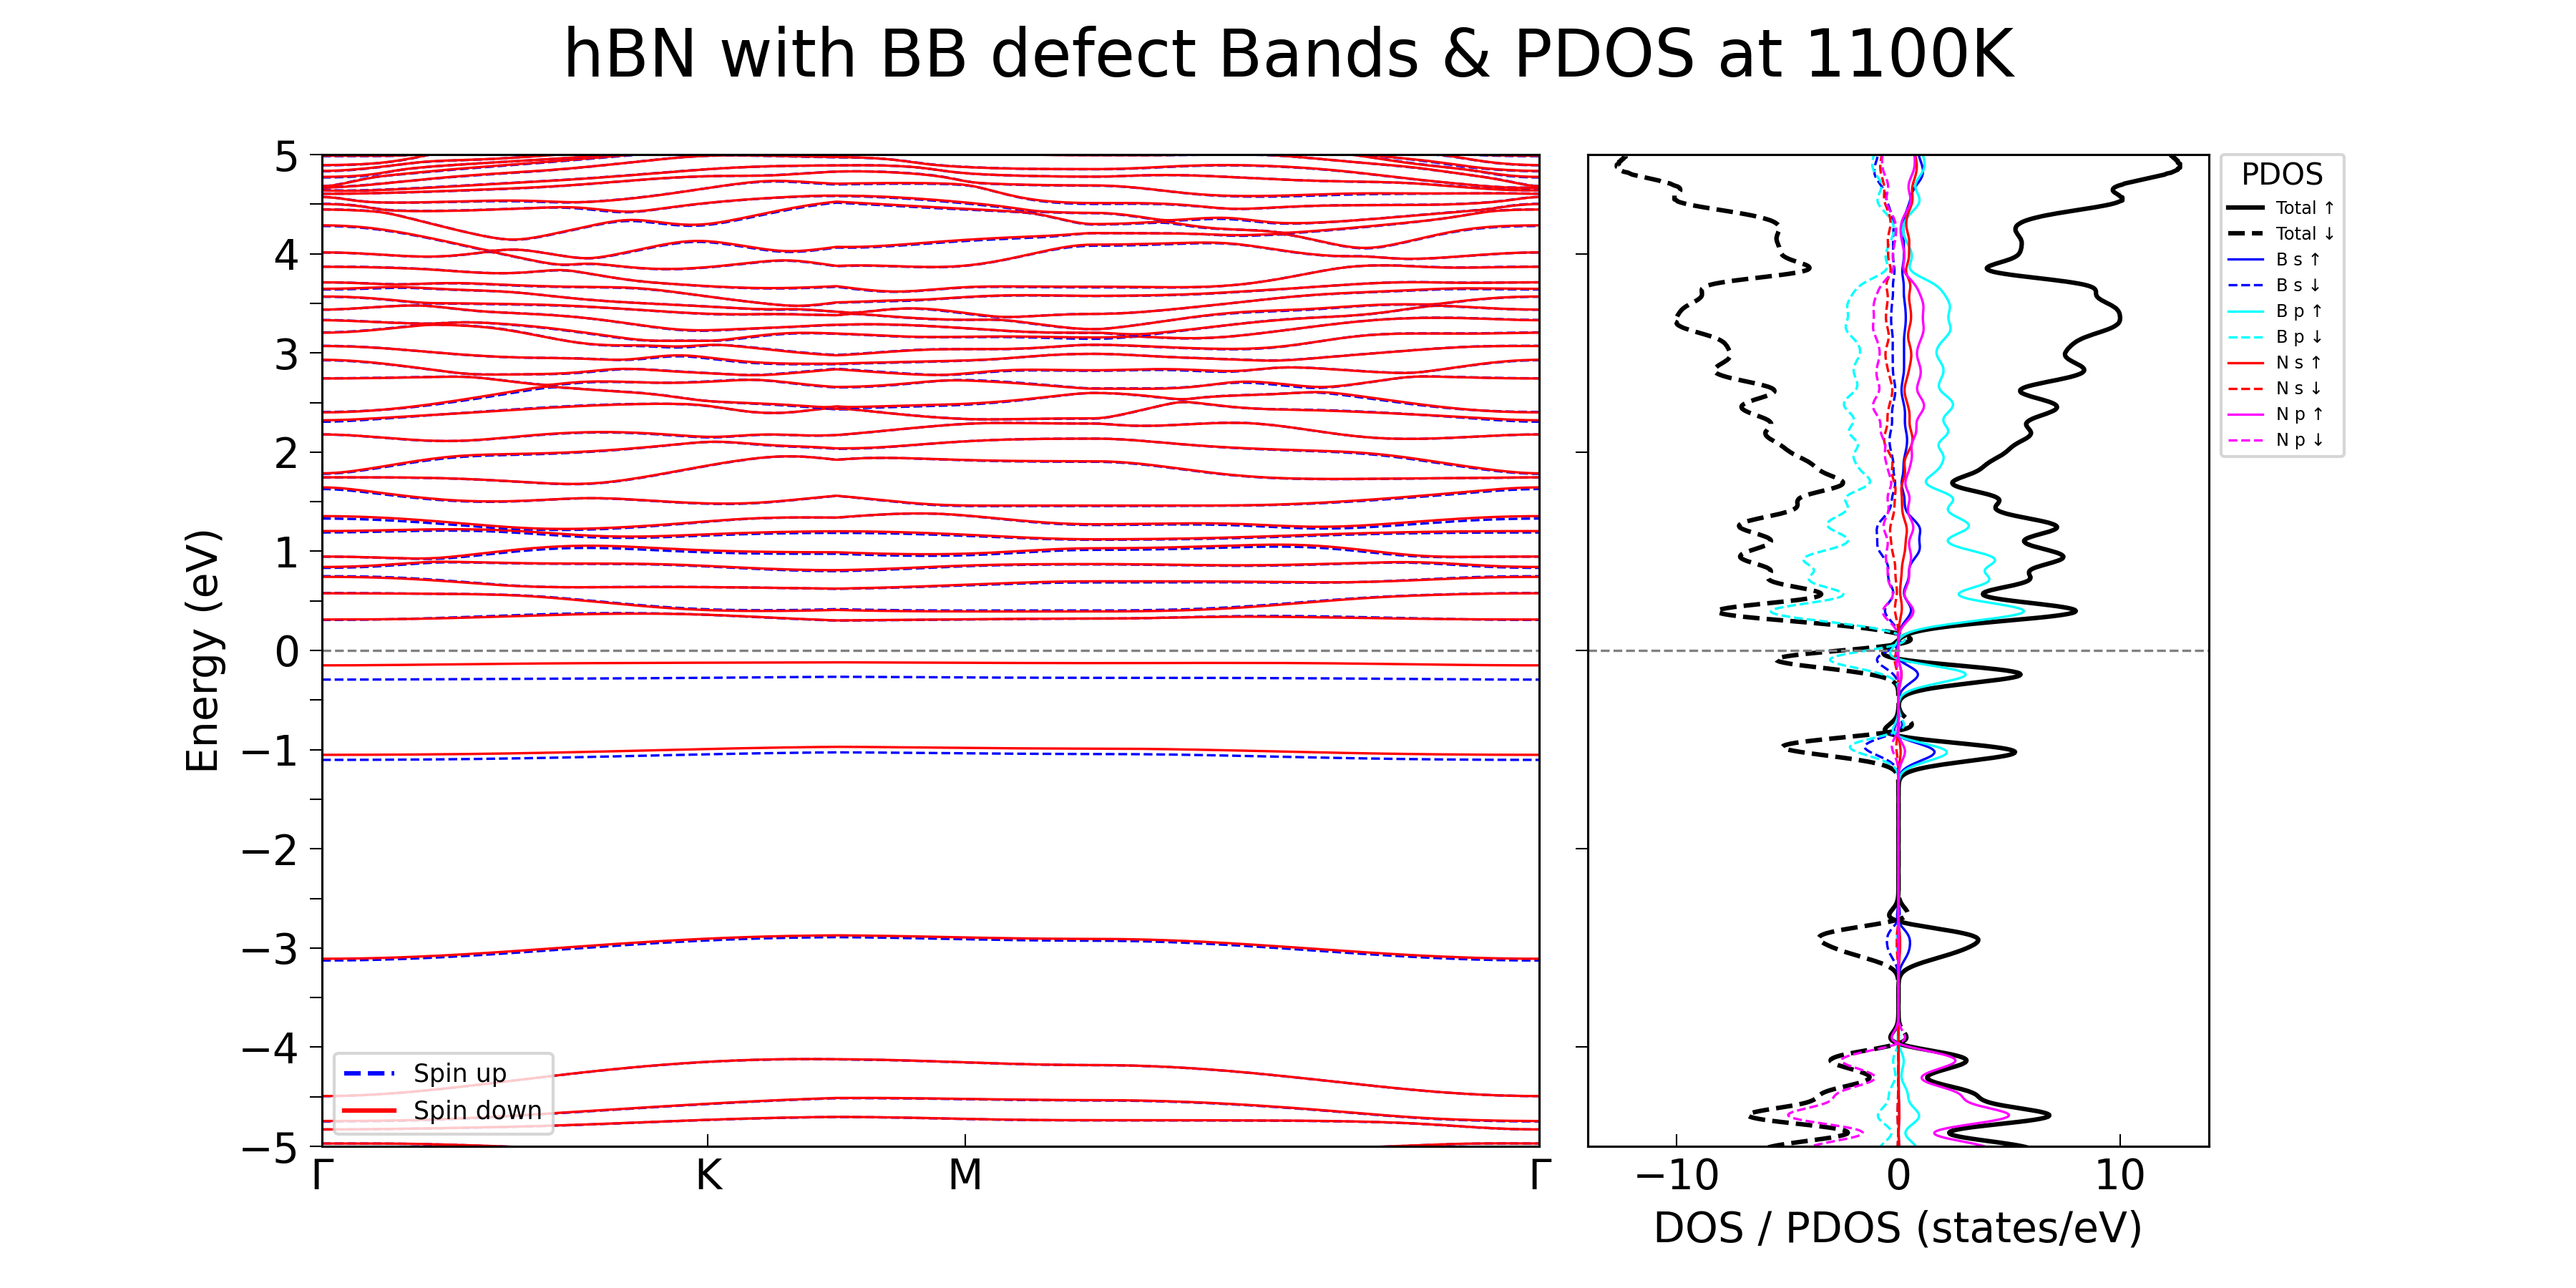
\includegraphics[width=0.95\textwidth]{gambar_hasil/simple_bands_pdos_BB_1100K.png}
    \caption{Struktur pita elektronik dan PDOS untuk monolayer hBN dengan cacat B\textsubscript{N} pada 1100 K. Terjadi pemisahan spin (kanal spin-atas dan spin-bawah berbeda), menandakan kemunculan magnetisme ($0.150 \mu_B$).}
    \label{fig:hbn_BB_1100K}
\end{figure}
\begin{figure}[htbp!] % PERUBAHAN: Ukuran gambar diperbesar
    \centering
    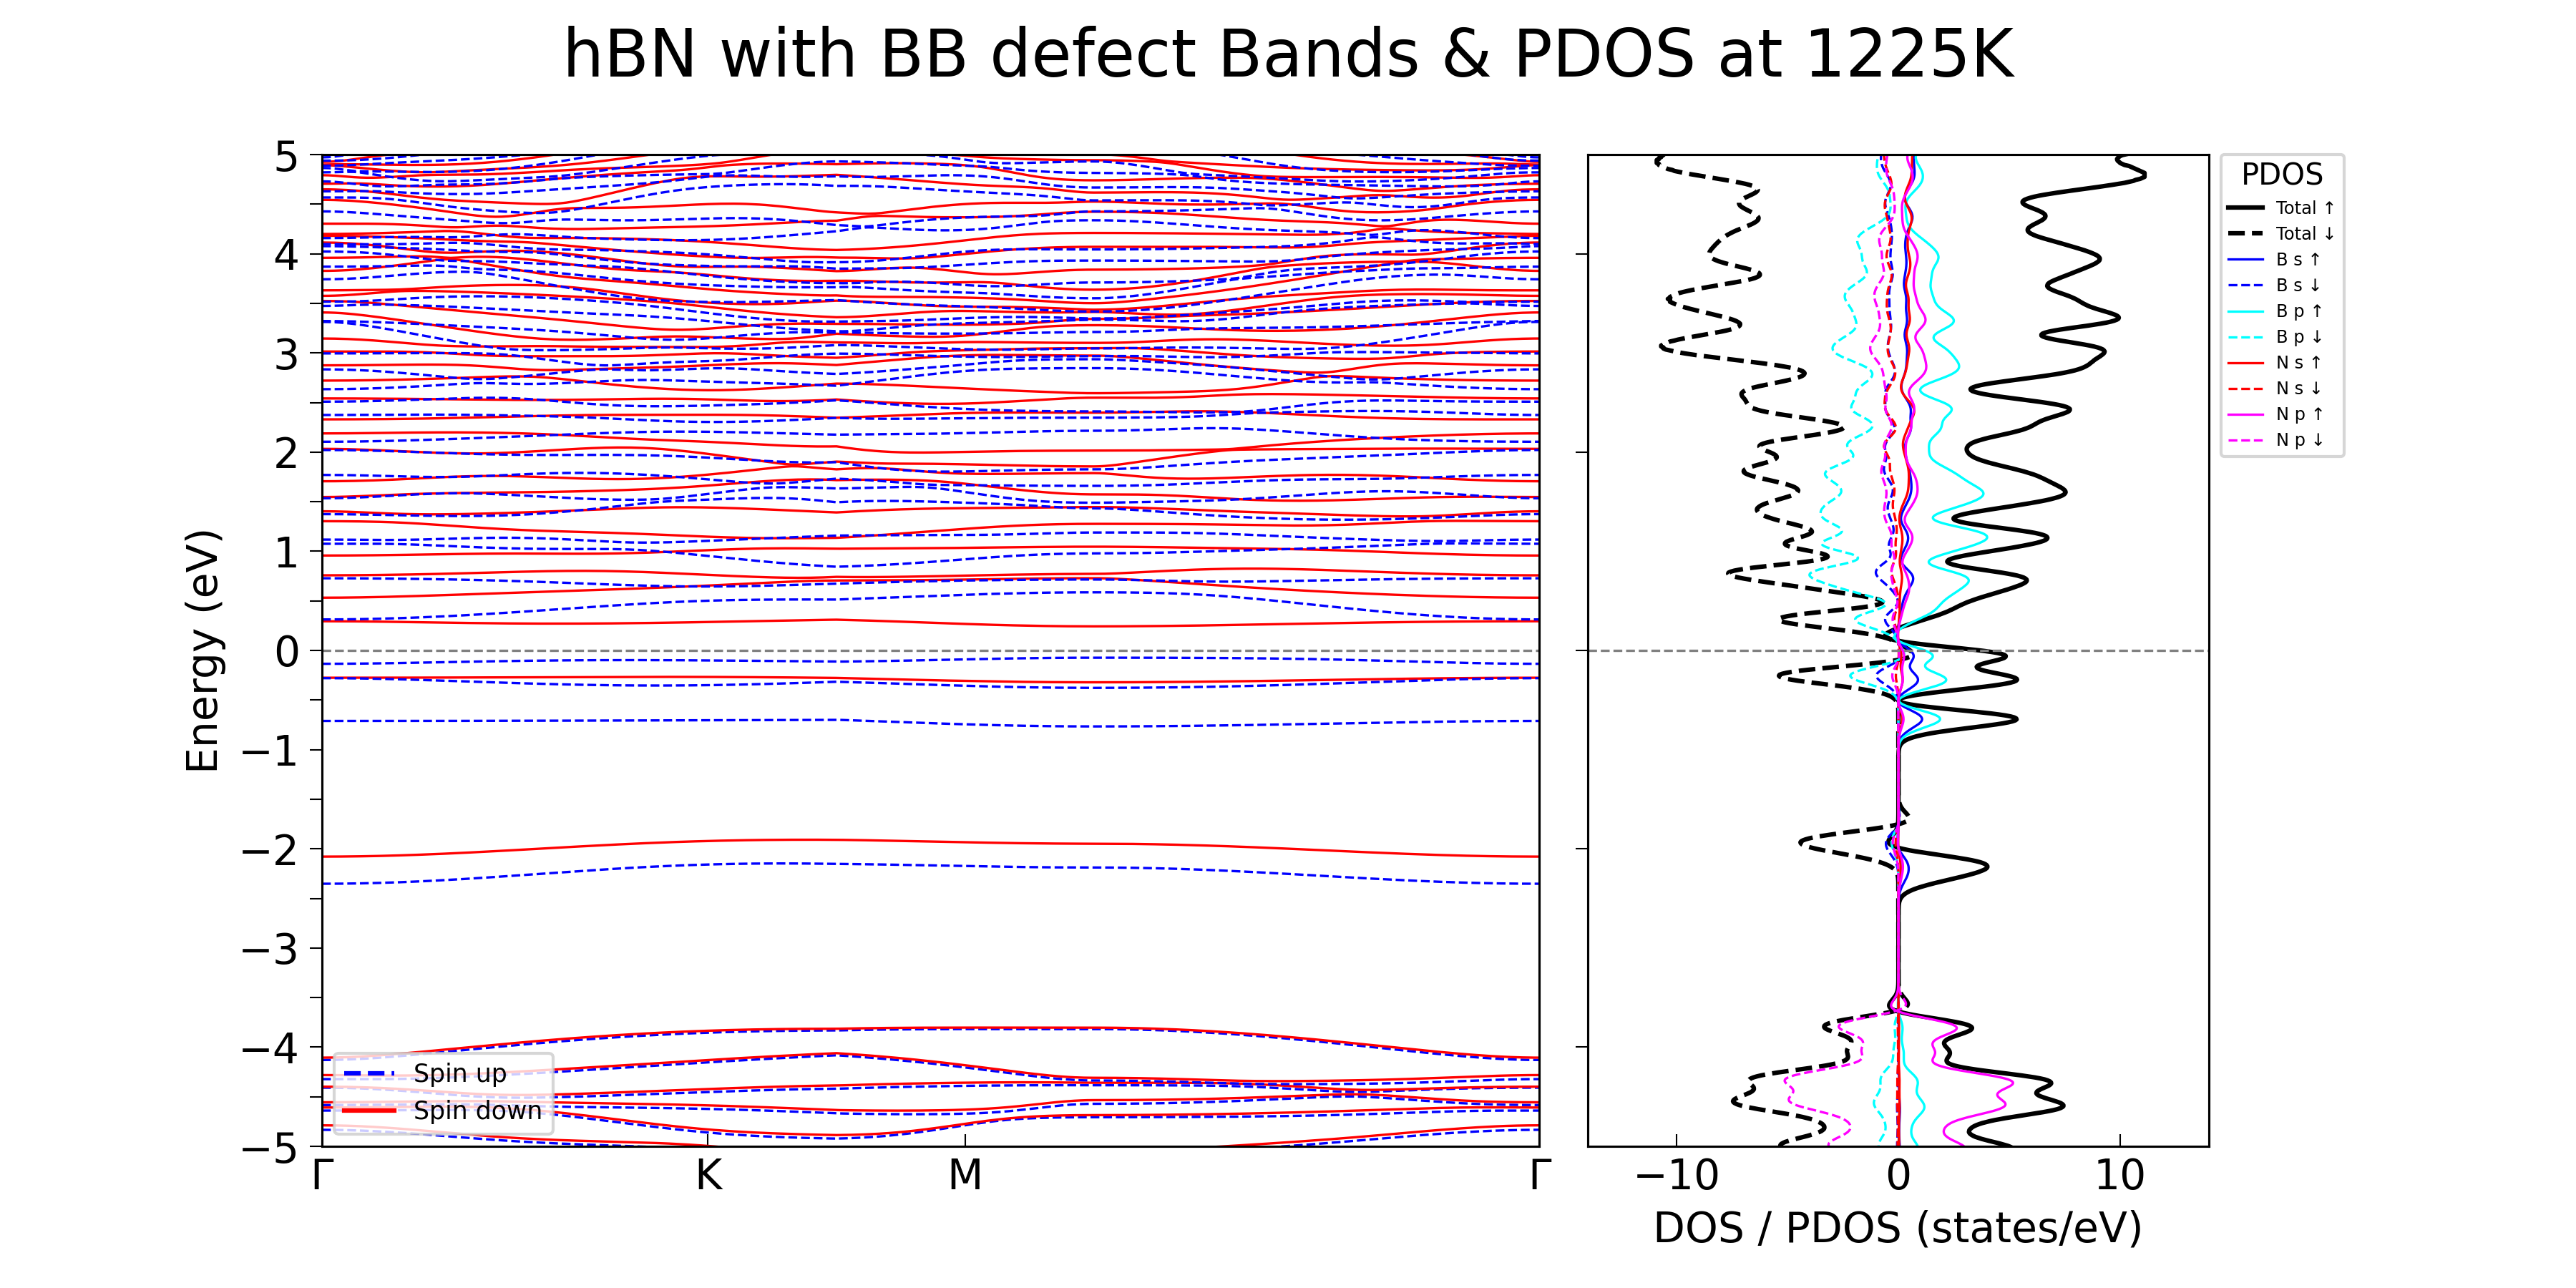
\includegraphics[width=0.95\textwidth]{gambar_hasil/simple_bands_pdos_BB_1225K.png}
    \caption{Struktur pita elektronik dan PDOS untuk monolayer hBN dengan cacat B\textsubscript{N} pada 1225 K. Pemisahan spin menjadi sangat signifikan, dengan magnetisasi total meningkat tajam menjadi $1.850 \mu_B$.}
    \label{fig:hbn_BB_1225K}
\end{figure}

Kemunculan magnetisme pada sistem yang hanya terdiri dari unsur-unsur blok-p ini dikenal sebagai magnetisme $d^0$ \citep{zhou2019}.
Magnetisme ini tidak berasal dari orbital $d$ atau $f$ yang terisi sebagian, melainkan dari polarisasi spin elektron-elektron $p$ yang terlokalisasi akibat ketidakseimbangan elektron dan ikatan tak jenuh (\emph{dangling bonds}) yang diciptakan oleh cacat.
Cacat B\textsubscript{N} menciptakan keadaan elektronik terlokalisasi di dekat tingkat Fermi, yang jika kerapatannya cukup tinggi, dapat memicu polarisasi spin spontan untuk menurunkan energi total sistem (kriteria Stoner).
Temuan yang paling luar biasa adalah \emph{peningkatan} magnetisasi dengan suhu, dari nol pada 800 K menjadi $1.850 \mu_B$ pada 1225 K. Perilaku ini sangat tidak konvensional, karena energi termal ($k_B T$) biasanya berfungsi mengacaukan tatanan magnetik.
Fenomena ini menunjuk pada adanya mekanisme kopling spin-fonon (SPC) yang kuat \citep{Liu_2025}.
Hipotesisnya adalah sebagai berikut:
\begin{enumerate}
    \item Pada 800 K, distorsi termal pada kisi belum cukup kuat untuk membuat keadaan dasar magnetik lebih stabil daripada keadaan non-magnetik.
\item Seiring meningkatnya temperatur ke 1100 K dan 1225 K, moda-moda fonon beramplitudo lebih besar menjadi aktif.
\item Moda-moda fonon spesifik ini berinteraksi kuat dengan keadaan spin elektronik di sekitar cacat B\textsubscript{N}.
\item Interaksi ini berarti vibrasi kisi tidak lagi bertindak sebagai sumber kekacauan, tetapi secara aktif \emph{menciptakan dan menstabilkan} distorsi struktural lokal (misalnya, pemanjangan ikatan atau pengerutan) yang kondusif untuk polarisasi spin.
\end{enumerate}
Dengan kata lain, fonon menjadi bahan aktif yang memediasi transisi menuju fasa magnetik.
Temperatur yang lebih tinggi mendorong sistem lebih dalam ke fase magnetik yang lebih teratur, sebuah contoh menakjubkan dari bagaimana interaksi kolektif dapat memunculkan tatanan yang tidak terduga \citep{Pantazopoulos2024}.

\subsubsection{Bukti Visual Kopling Spin-Fonon dari Kerapatan Muatan dan Spin}
\label{subsec:hbn_BB_density_analysis}
Analisis kerapatan muatan dan spin untuk sistem B\textsubscript{N} (Gambar \ref{fig:hbn_BB_density}) memberikan bukti visual yang paling meyakinkan untuk mekanisme magnetisme yang diinduksi oleh temperatur.
Plot-plot ini menyajikan narasi visual tentang transisi fasa dari keadaan non-magnetik ke keadaan magnetik yang kuat.
\begin{figure}[htbp!] % PERUBAHAN: Ukuran gambar diperbesar
  \centering
  \begin{subfigure}[b]{0.49\textwidth}
    \centering
    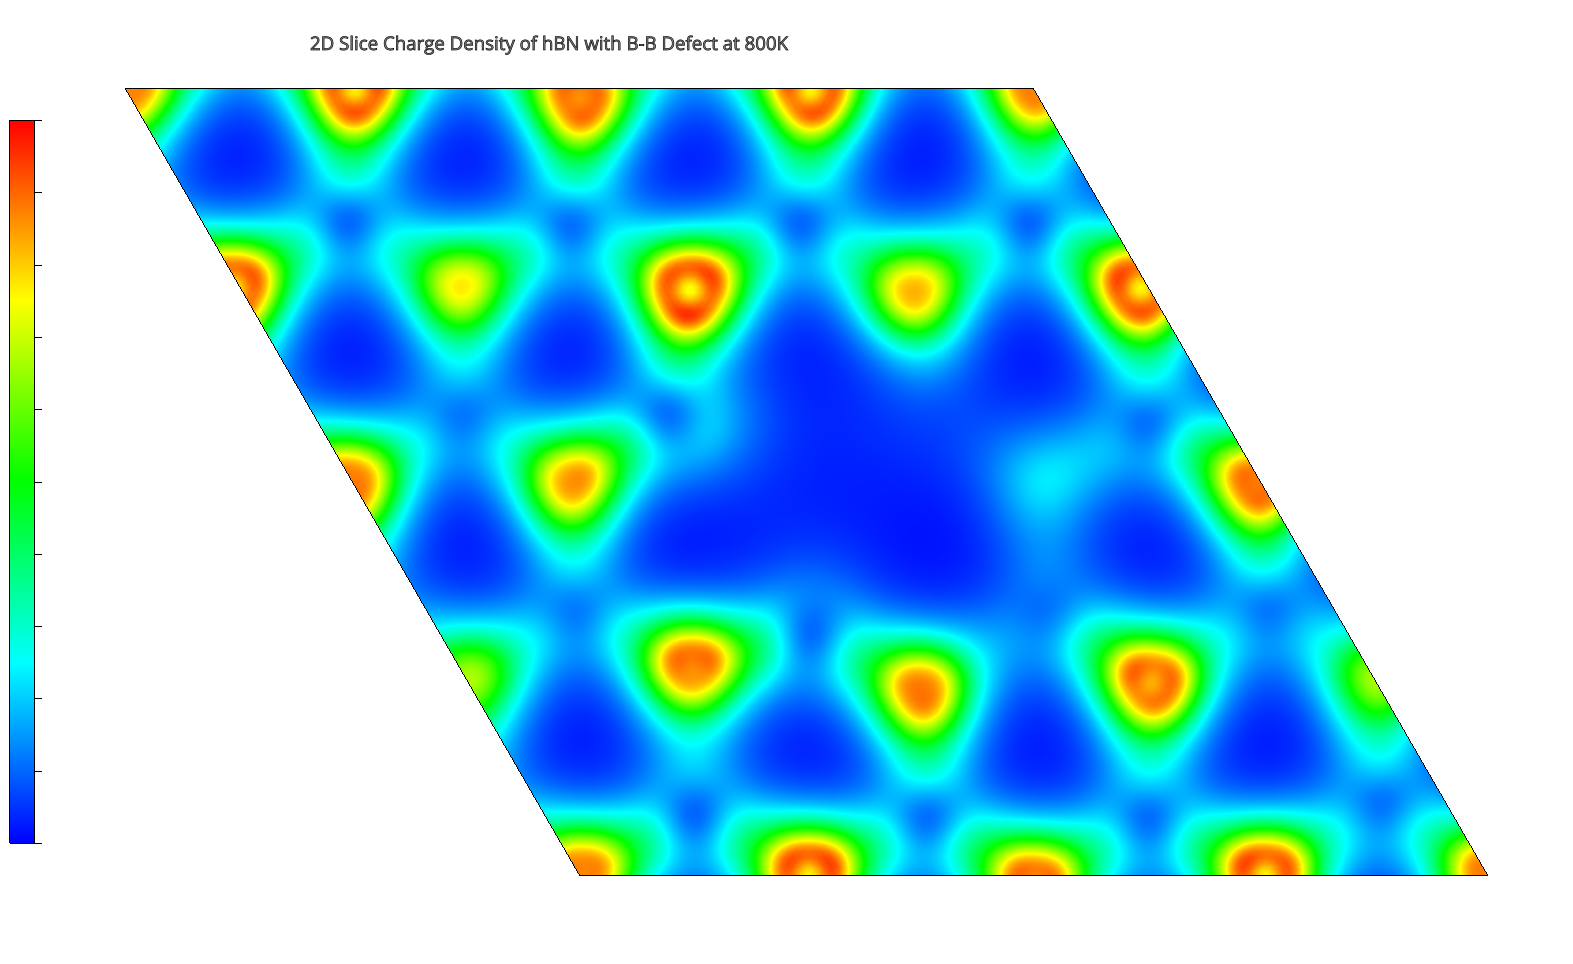
\includegraphics[width=\linewidth]{hBN_rho_BB_800K.png}
    \caption{Kerapatan Muatan, 800 K}
    \label{subfig:rho_bb_800k}
  \end{subfigure}\hfill
  \begin{subfigure}[b]{0.49\textwidth}
    \centering
    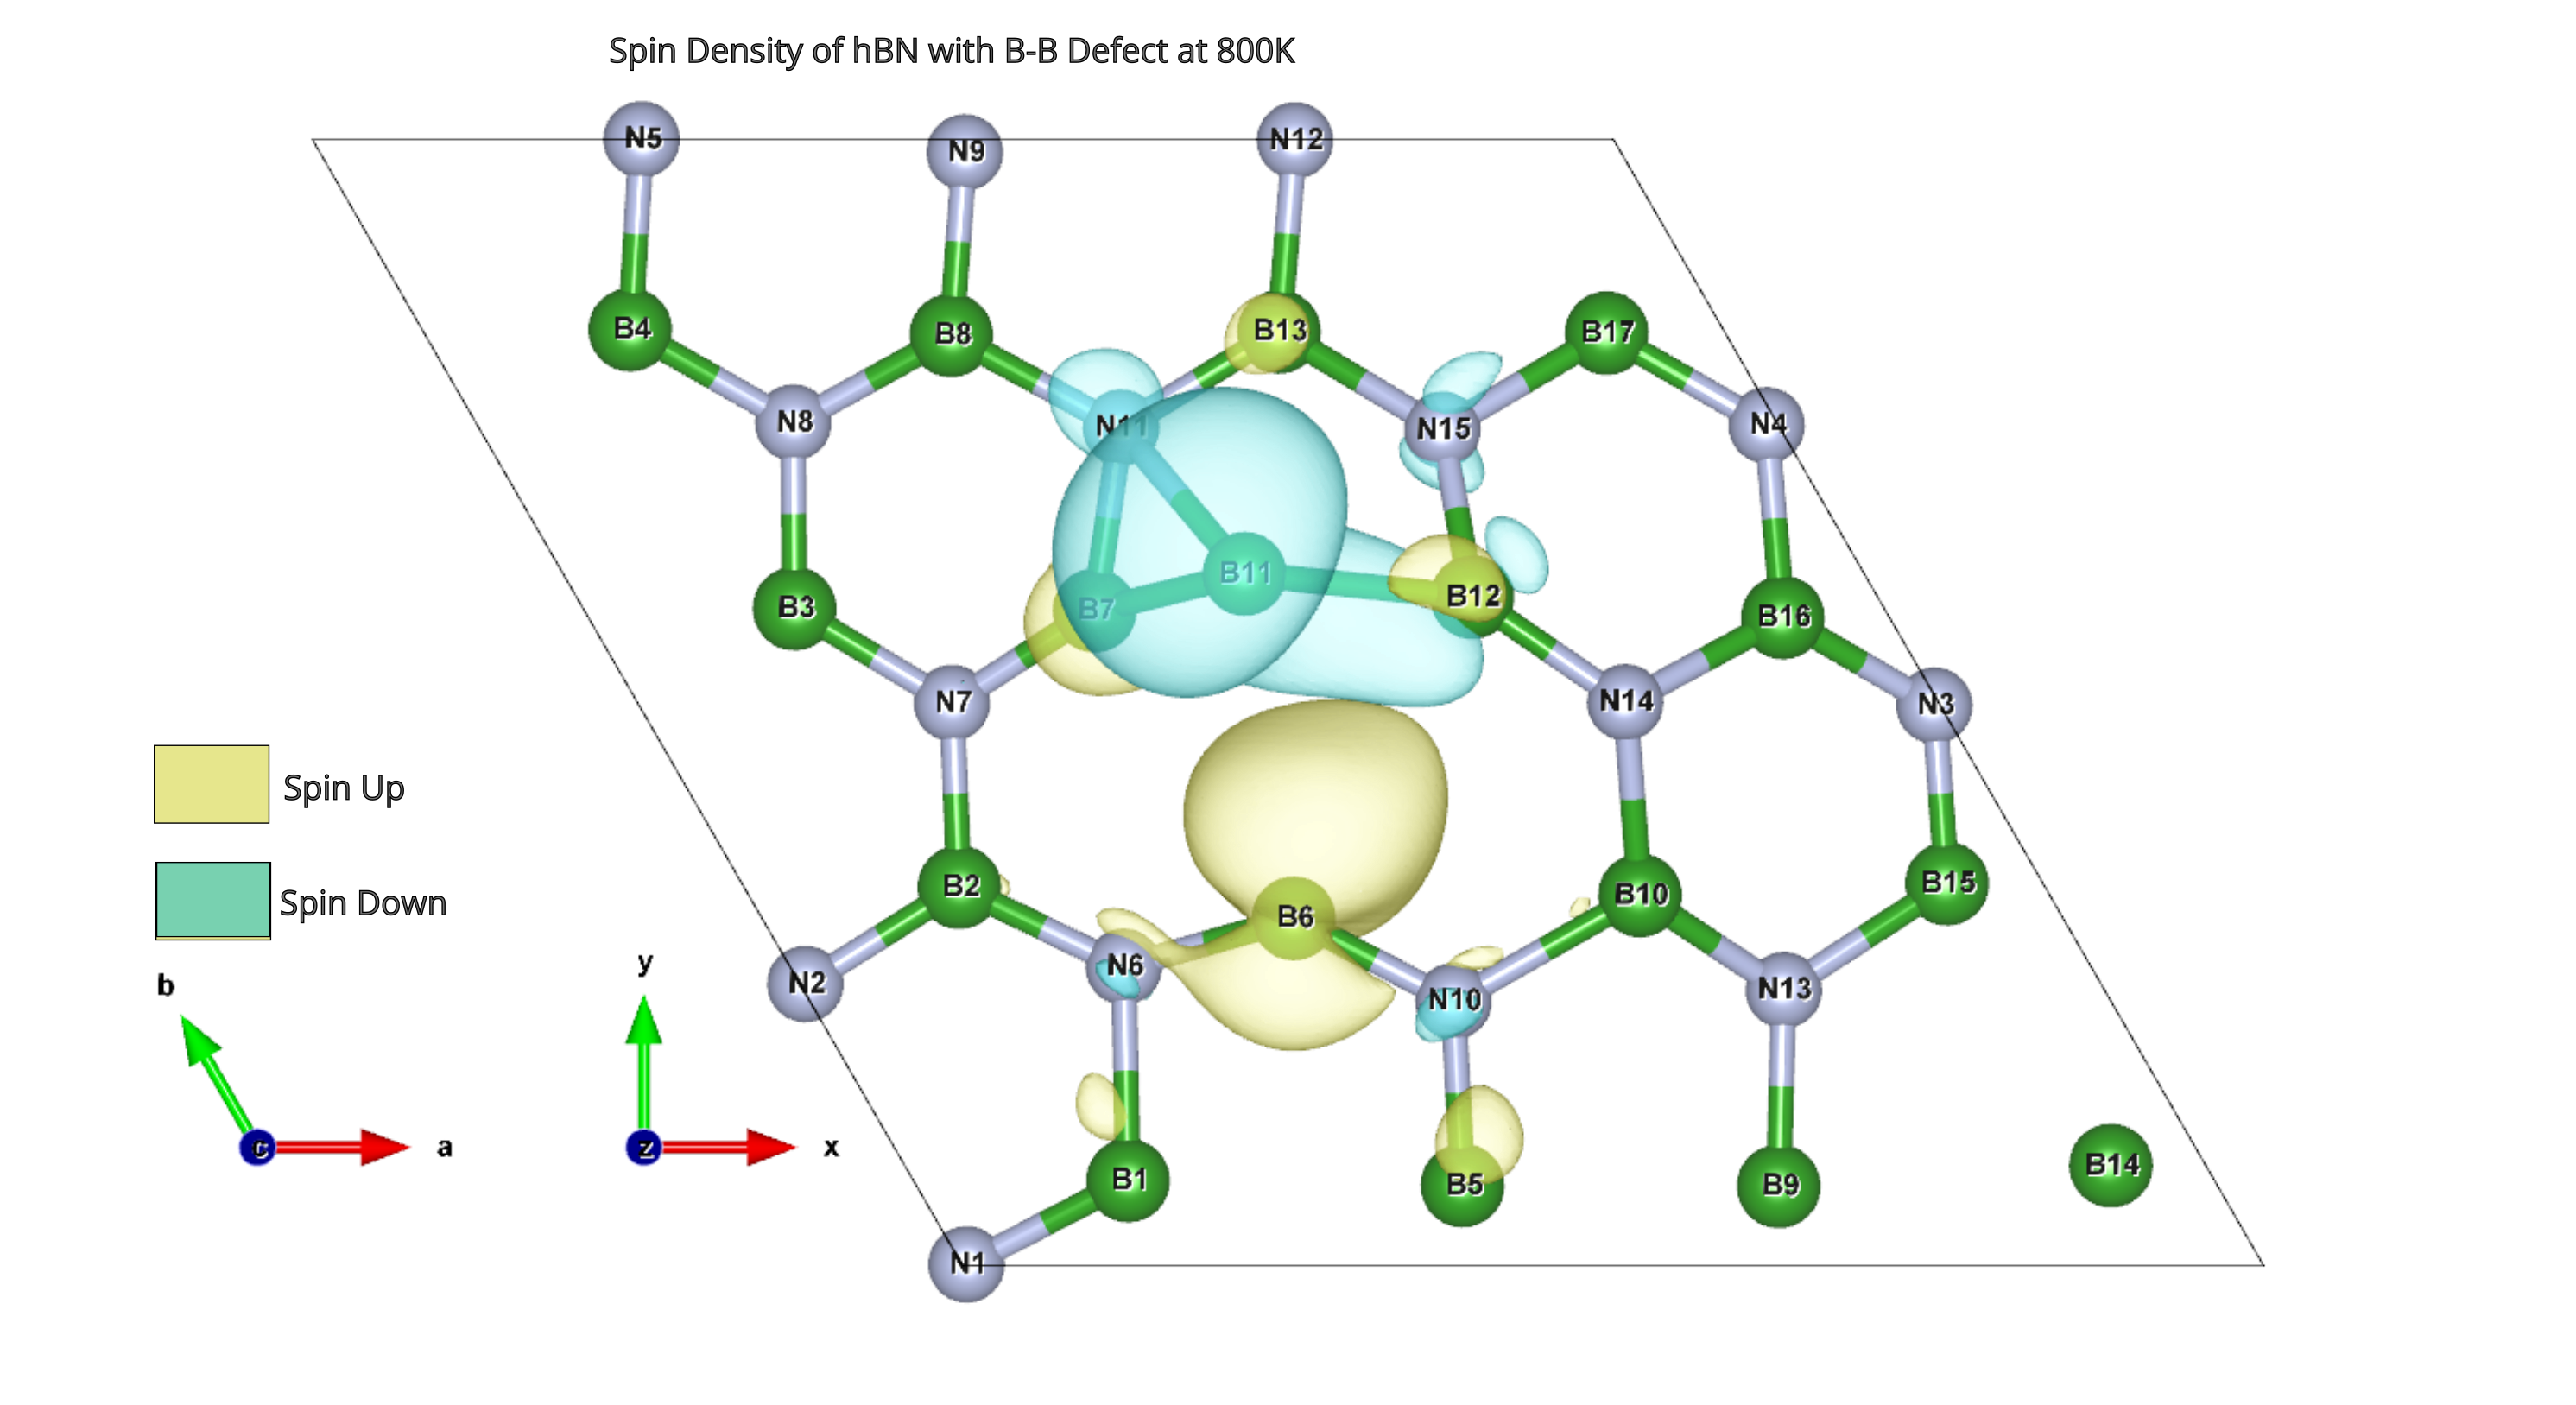
\includegraphics[width=\linewidth]{hBN_spin_BB_800K.png}
    \caption{Kerapatan Spin, 800 K}
    \label{subfig:spin_bb_800k}
  \end{subfigure}
  \vspace{1em}

  \begin{subfigure}[b]{0.49\textwidth}
    \centering
    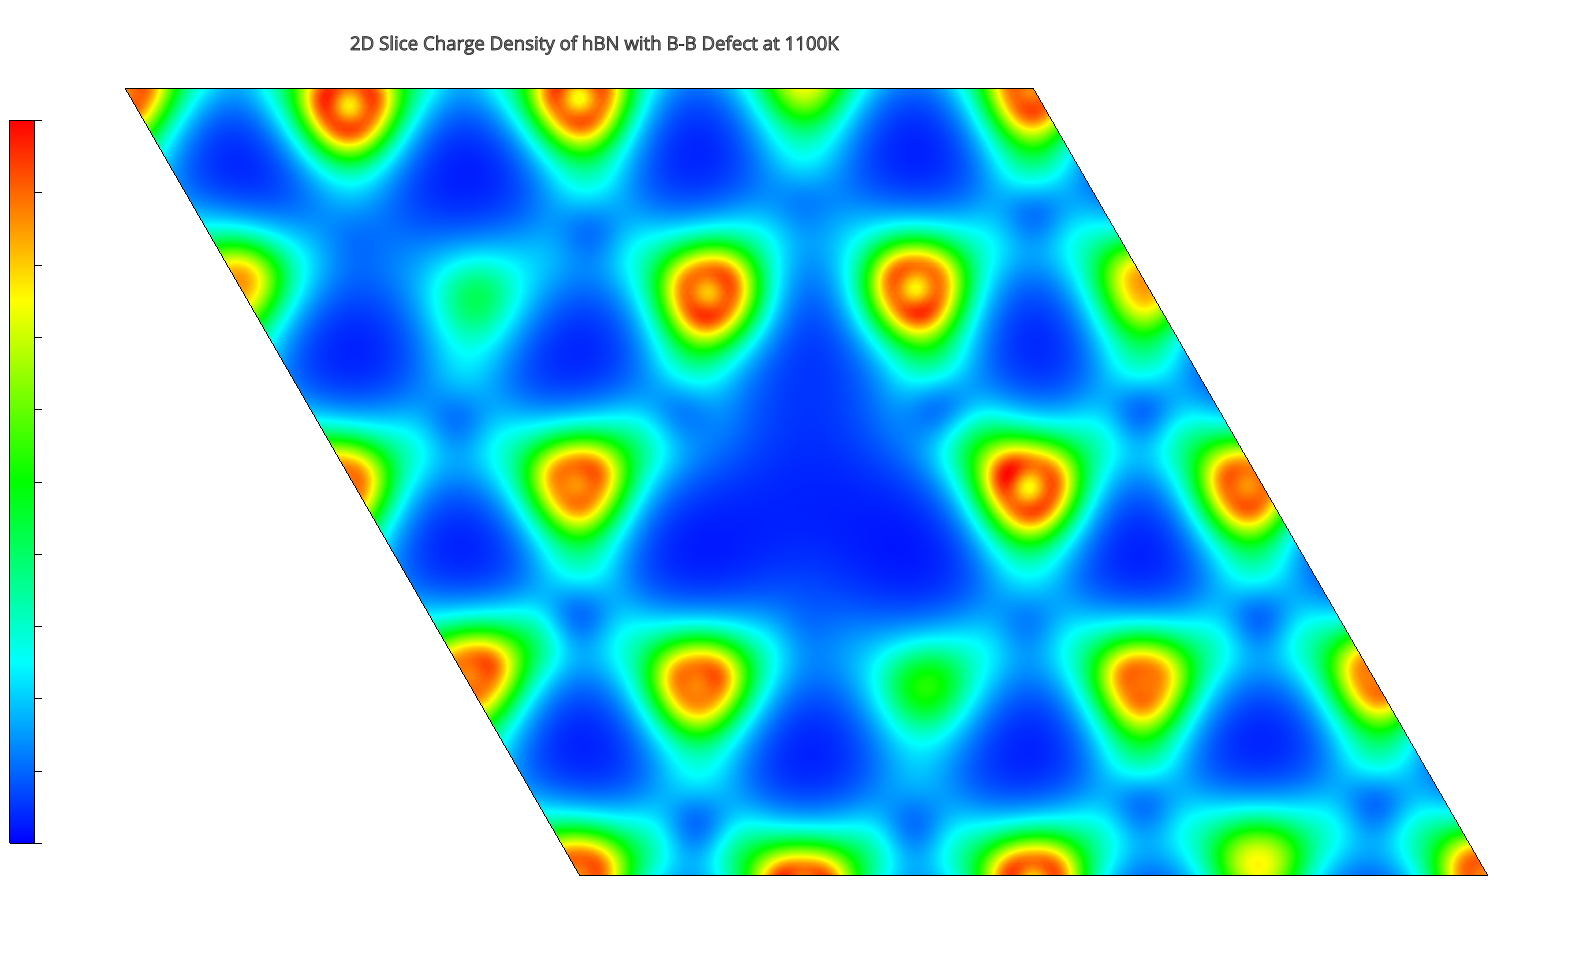
\includegraphics[width=\linewidth]{hBN_rho_BB_1100K.png}
    \caption{Kerapatan Muatan, 1100 K}
    \label{subfig:rho_bb_1100k}
  \end{subfigure}\hfill
  \begin{subfigure}[b]{0.49\textwidth}
    \centering
    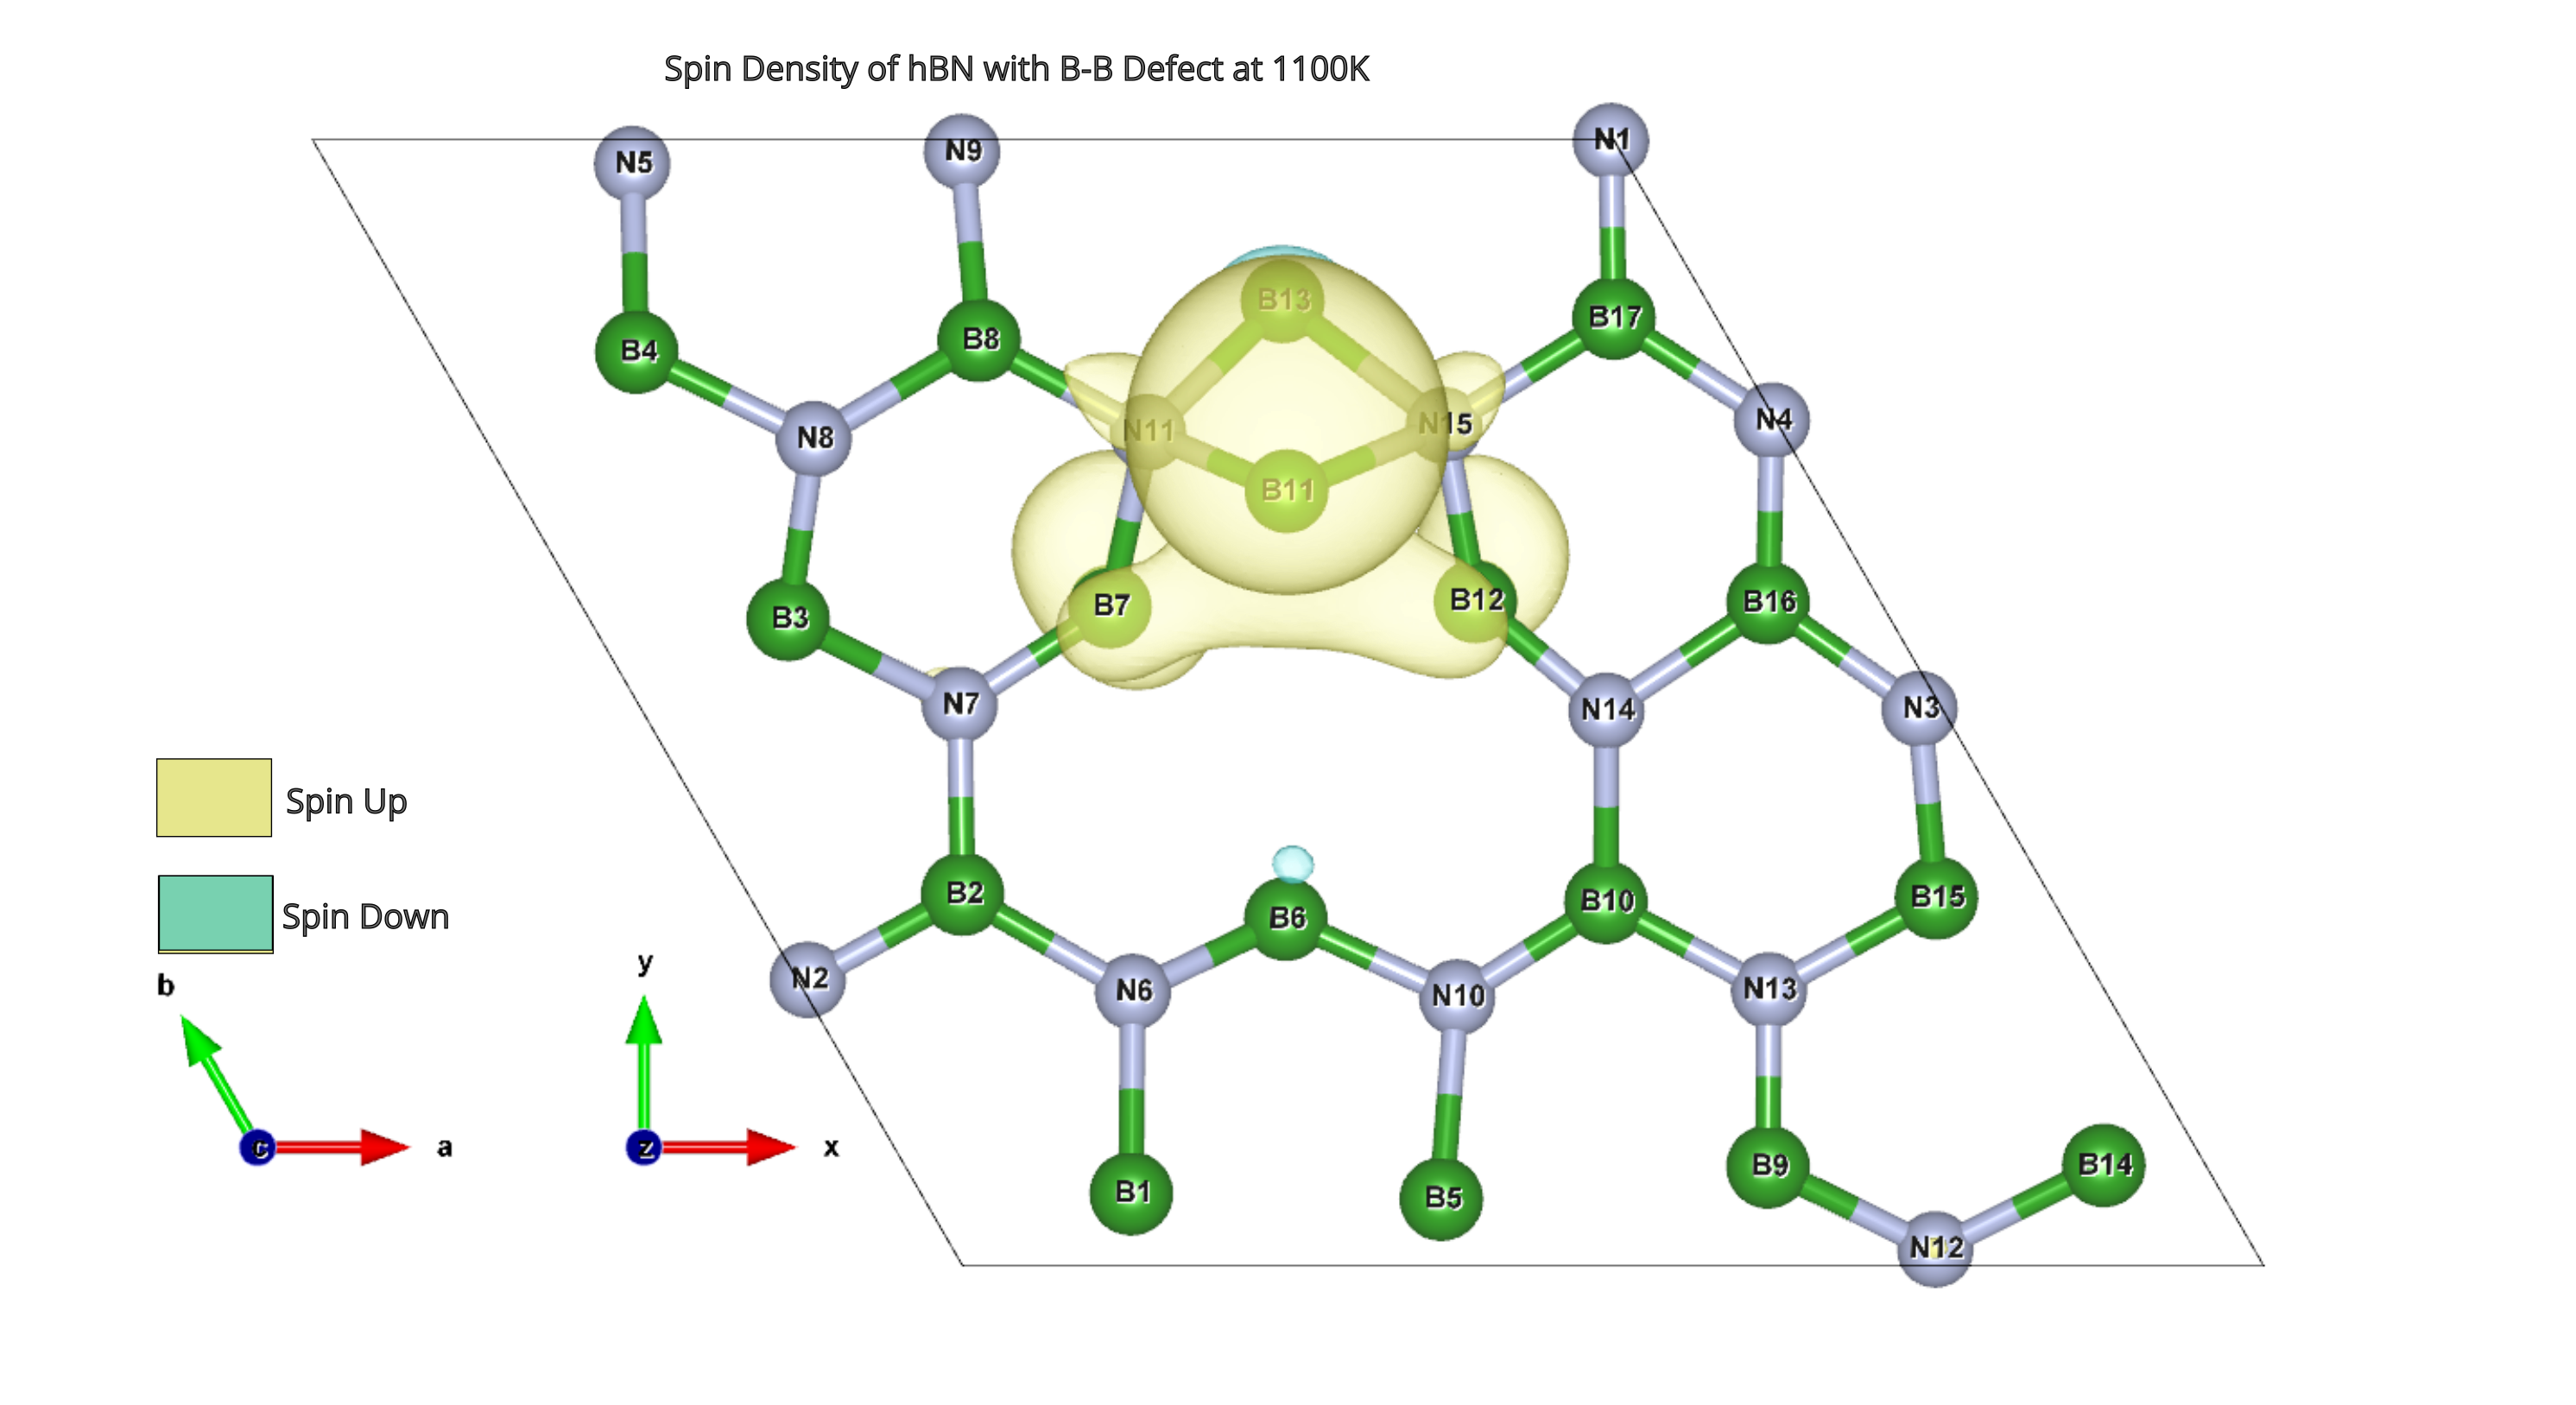
\includegraphics[width=\linewidth]{hBN_spin_BB_1100K.png}
    \caption{Kerapatan Spin, 1100 K}
    \label{subfig:spin_bb_1100k}
  \end{subfigure}
  \vspace{1em}

  \begin{subfigure}[b]{0.49\textwidth}
    \centering
    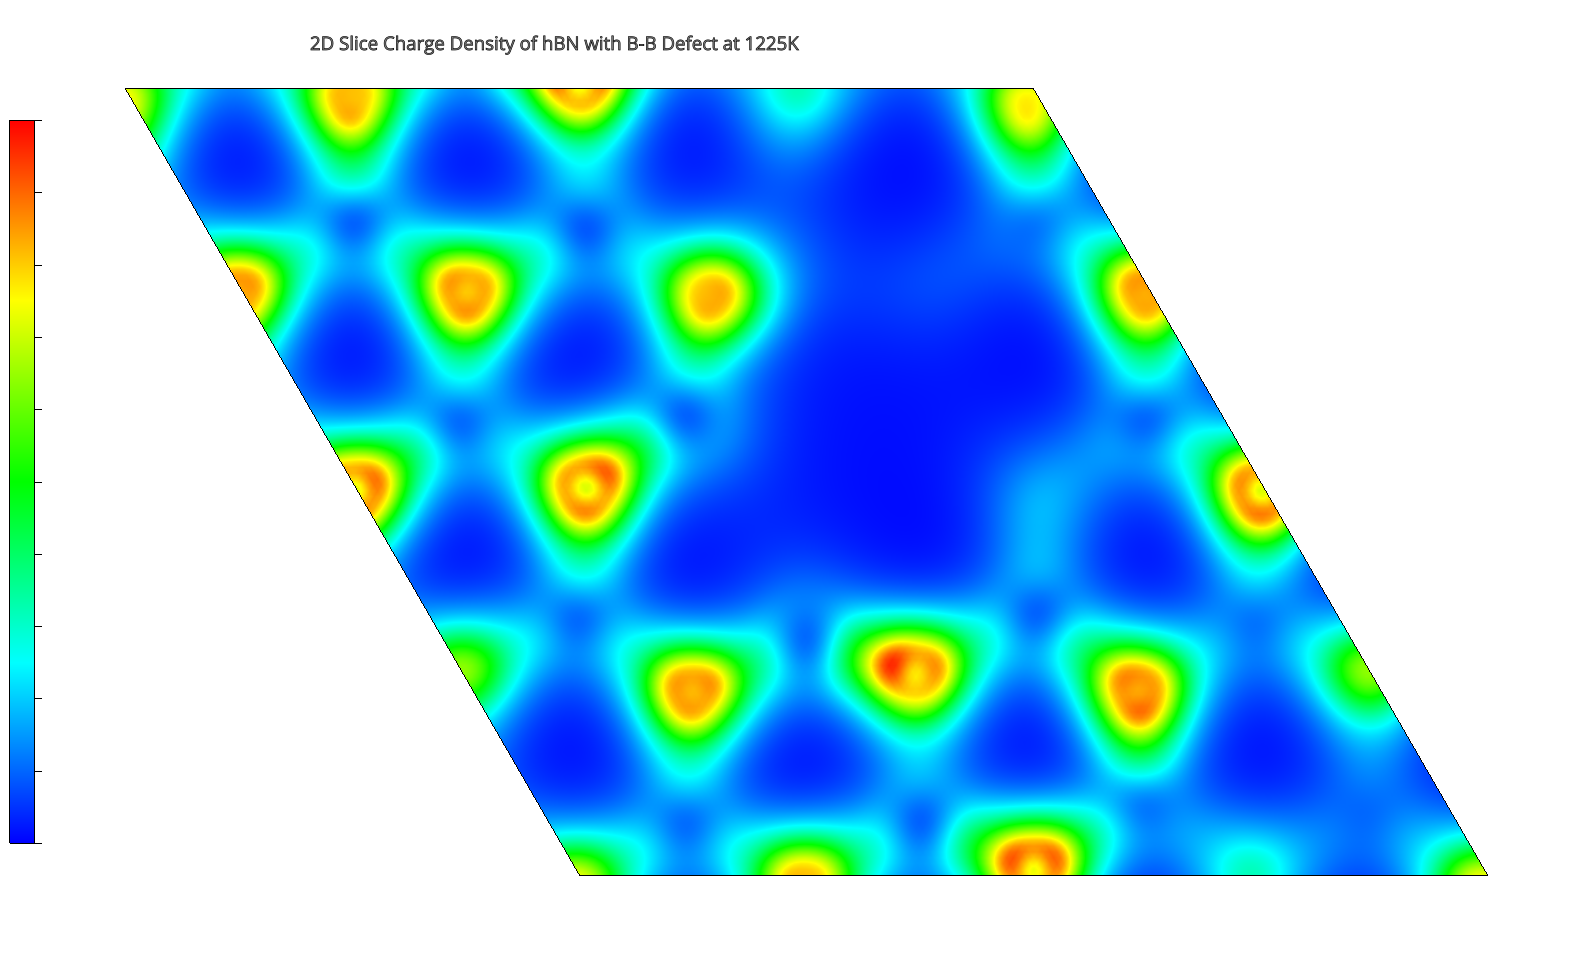
\includegraphics[width=\linewidth]{hBN_rho_BB_1225K.png}
    \caption{Kerapatan Muatan, 1225 K}
    \label{subfig:rho_bb_1225k}
  \end{subfigure}\hfill
  \begin{subfigure}[b]{0.49\textwidth}
    \centering
    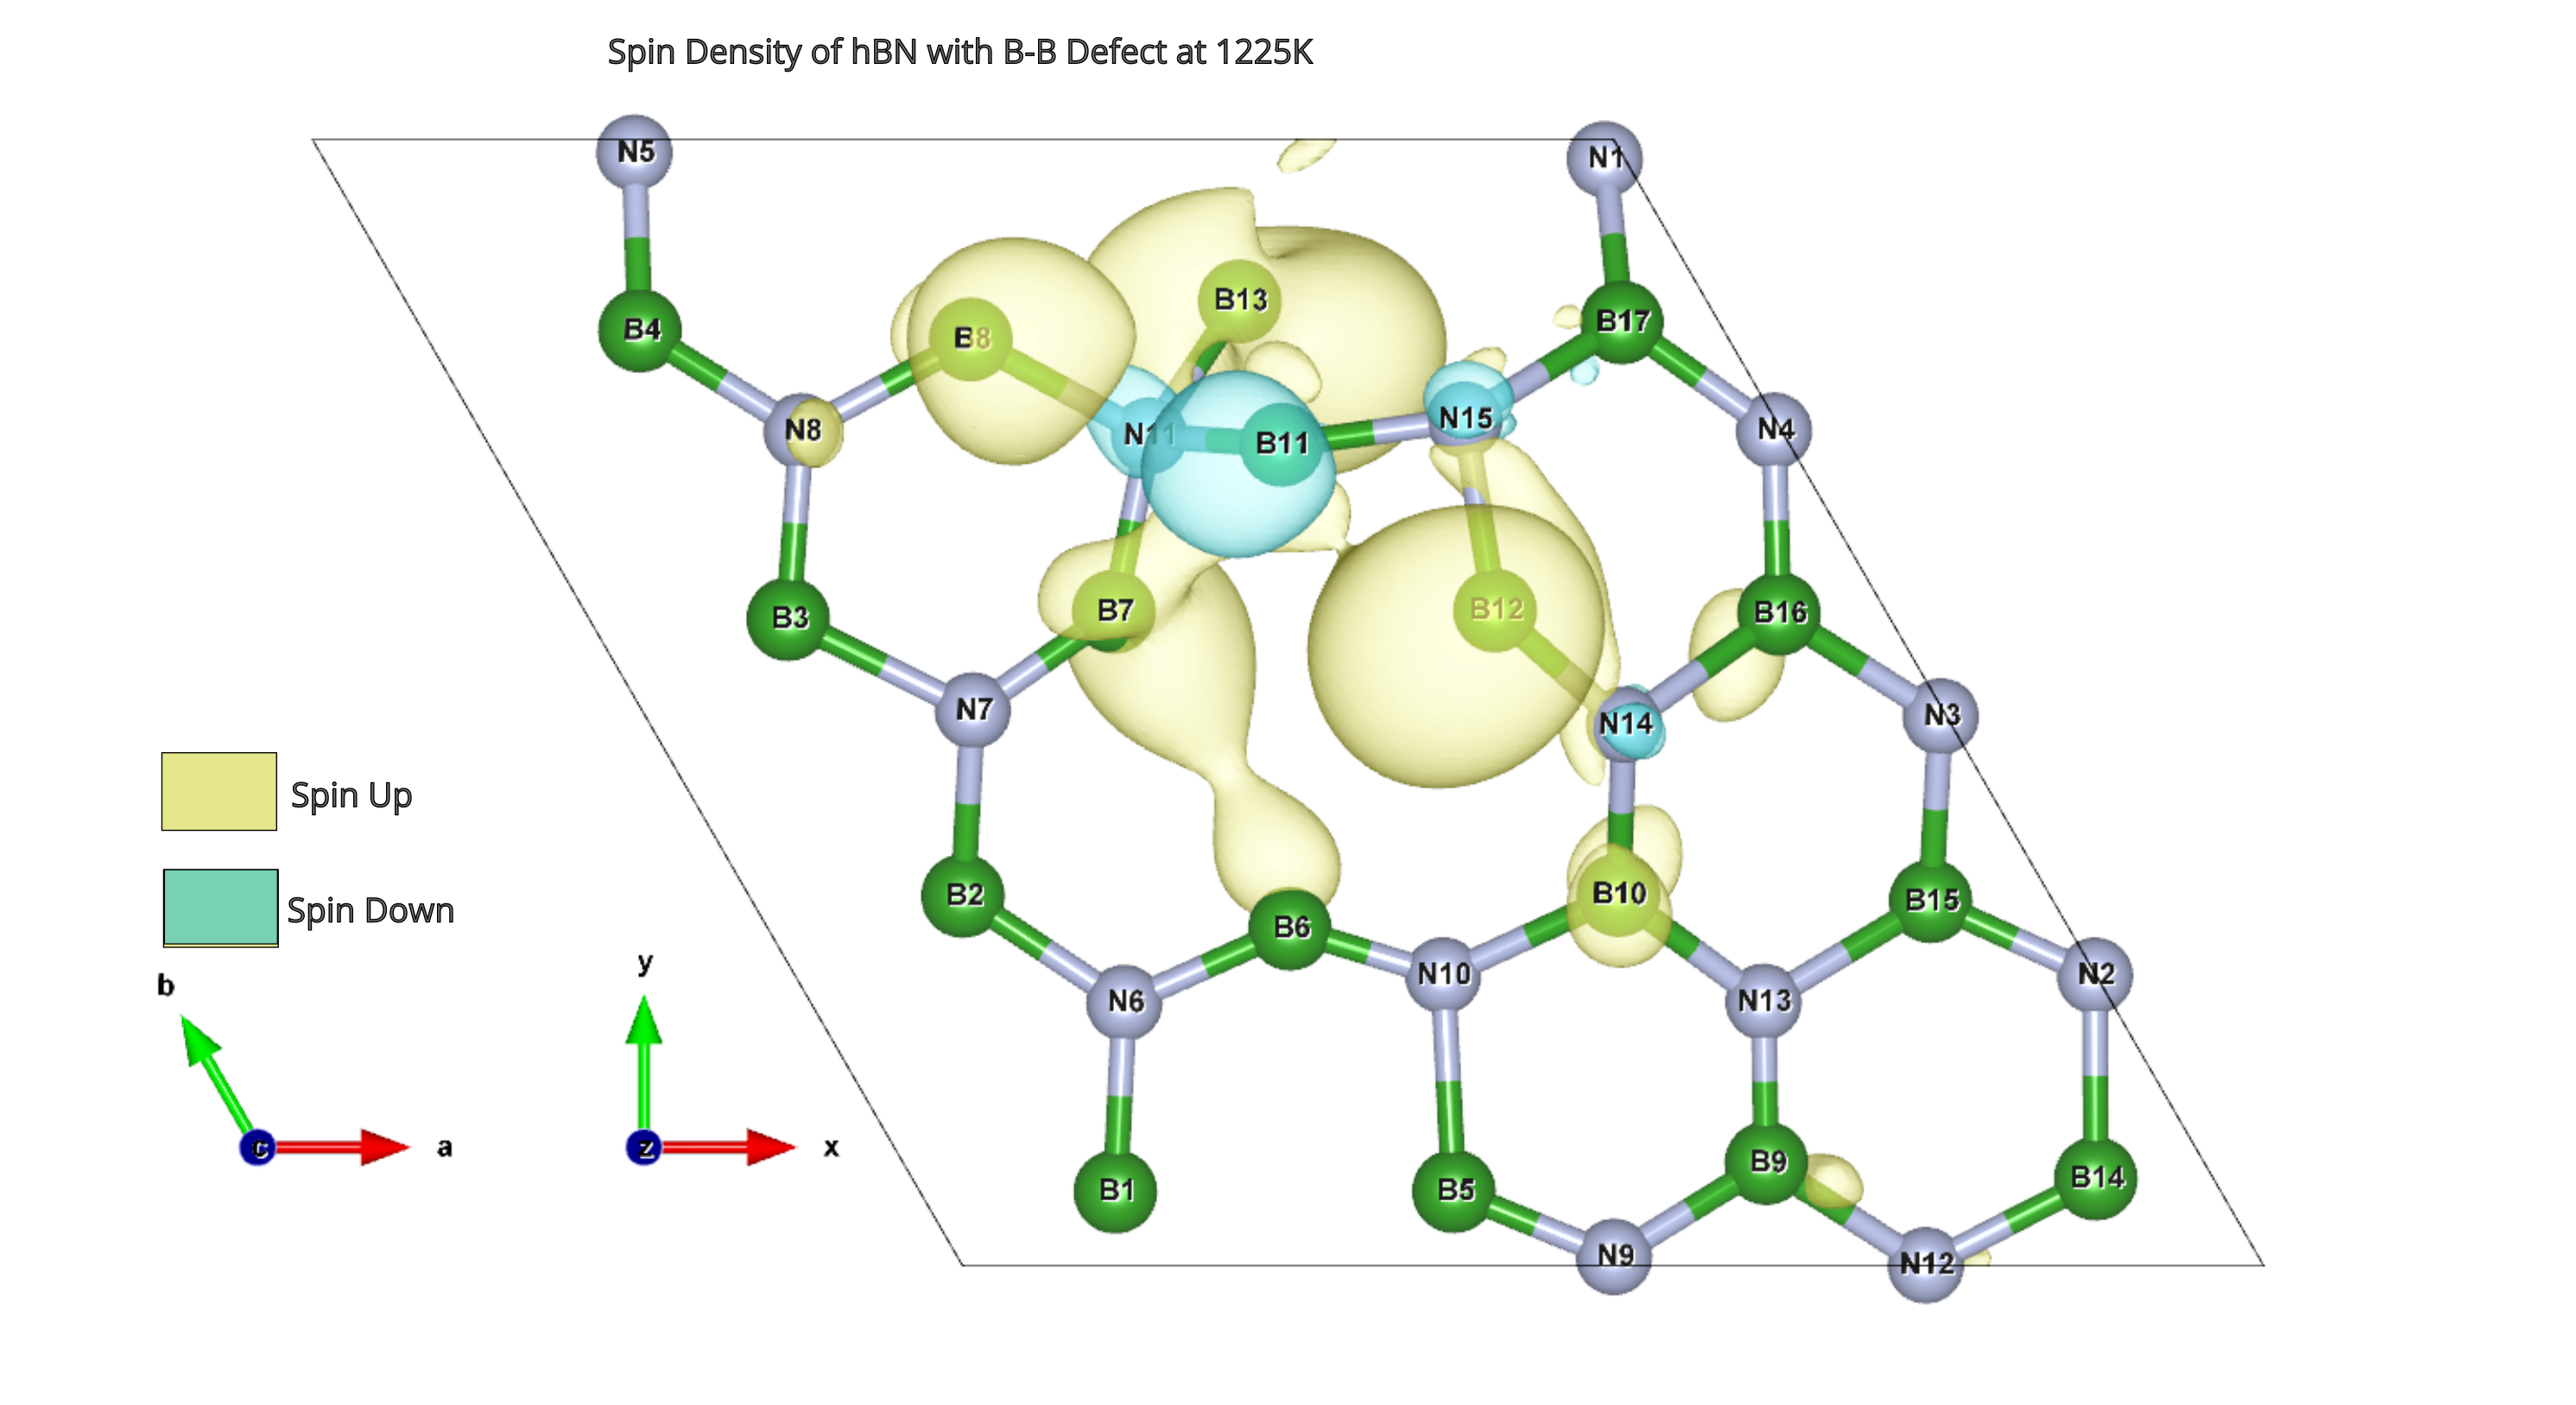
\includegraphics[width=\linewidth]{hBN_spin_BB_1225K.png}
    \caption{Kerapatan Spin, 1225 K}
    \label{subfig:spin_bb_1225k}
  \end{subfigure}
  \caption{Visualisasi 2D dari kerapatan muatan (kiri) dan kerapatan spin (kanan) untuk monolayer hBN dengan cacat B\textsubscript{N}. Warna merah pada kerapatan muatan menunjukkan akumulasi elektron, sedangkan warna biru menunjukkan deplesi. Untuk kerapatan spin, warna biru menunjukkan spin down dan warna kuning menunjukan spin up.}
  \label{fig:hbn_BB_density}
\end{figure}

Plot kerapatan muatan (Gambar \ref{fig:hbn_BB_density}a, c, e) menyoroti lingkungan elektronik yang sangat tidak stabil yang diciptakan oleh cacat B\textsubscript{N}.
Pembentukan ikatan B-B dan keberadaan atom nitrogen di sekitarnya yang kurang terkoordinasi menciptakan keadaan elektronik yang "tidak jenuh".
Lingkungan inilah yang rentan terhadap pemisahan spin, menyediakan keadaan sempit dengan kerapatan tinggi di dekat tingkat Fermi yang diperlukan untuk magnetisme $d^0$.
Naratif sesungguhnya terungkap dalam plot kerapatan spin. Pada 800 K (Gambar \ref{fig:hbn_BB_density}b), kerapatan spin adalah nol, yang secara visual mengonfirmasi keadaan dasar non-magnetik sistem, sejalan dengan data pada Tabel \ref{tab:hbn_defek_bn}.
Pada temperatur ini, energi termal tidak cukup untuk memicu mekanisme kopling spin-fonon.
Sebuah transisi dramatis terjadi pada 1100 K (Gambar \ref{fig:hbn_BB_density}d). Di sini, kita menyaksikan \emph{kemunculan} polarisasi spin.
Kantong-kantong kerapatan spin-atas (merah) dan spin-bawah (biru) yang terlokalisasi muncul, terutama pada atom-atom nitrogen yang bertetangga dengan situs cacat B\textsubscript{N}.
Ini adalah "bukti tak terbantahkan" (\emph{smoking gun}) dari onset magnetisme $d^0$, yang secara visual menunjukkan bahwa momen magnetik berasal dari polarisasi orbital $p$ pada atom-atom non-logam ini.
Ini adalah bukti visual pertama bahwa temperatur mulai \emph{menginduksi} tatanan magnetik, bukan menghancurkannya.
Pada 1225 K (Gambar \ref{fig:hbn_BB_density}f), fenomena ini mengalami \emph{amplifikasi} yang signifikan.
Intensitas warna (menunjukkan besarnya polarisasi spin) dan jangkauan spasial dari daerah yang terpolarisasi spin meningkat secara dramatis.
Ini memberikan bukti visual yang tak terbantahkan untuk hipotesis kopling spin-fonon.
Peningkatan energi termal menggerakkan moda fonon beramplitudo lebih besar—sebuah fenomena yang telah diisyaratkan oleh nilai MSD yang tinggi untuk sistem ini (Bagian \ref{subsec:md_rdf_msd}).
Alih-alih mengacaukan tatanan magnetik, vibrasi-vibrasi ini secara aktif menstabilkan distorsi geometris lokal yang tidak hanya memungkinkan tetapi juga \emph{memperkuat} polarisasi spin.
Fenomena kontra-intuitif di mana "gangguan" (vibrasi termal) mengarah pada "tatanan" (magnetisme) kini terkonfirmasi secara visual.

\section{Keterkaitan antara Dinamika Struktur, Stabilitas Termal, dan Sifat Kuantum}
\label{sec:diskusi_komprehensif}
Analisis yang telah dipaparkan mengungkapkan sebuah narasi yang kaya tentang bagaimana struktur, stabilitas, dan sifat kuantum saling terkait erat dalam monolayer hBN.
Dengan menggabungkan wawasan dari simulasi MD dan kalkulasi DFT, kita dapat membangun gambaran komprehensif tentang fisika yang mendasari perilaku material ini di bawah pengaruh temperatur dan cacat.
\subsection{Korelasi Struktur-Sifat: Dari RDF dan MSD ke Elektronik}
\label{subsec:korelasi_struktur_md_dft}
Alur kerja multi-skala yang digunakan dalam penelitian ini menyoroti hubungan sebab-akibat yang krusial: dinamika struktural pada skala pikosekon (ditangkap oleh MD) secara langsung menentukan sifat elektronik keadaan dasar (dihitung oleh DFT).
\begin{itemize}
    \item Untuk hBN murni, analisis RDF dan MSD (Bagian \ref{subsec:md_rdf_msd}) menunjukkan sistem yang relatif teratur dan stabil.
Sifat elektronik yang dihasilkan (Bagian \ref{subsec:hbn_murni_termal}) mencerminkan respons "global" dari kisi yang teratur ini terhadap eksitasi termal, yaitu pergeseran merah normal yang didorong oleh kopling elektron-fonon.
Ketiadaan polarisasi spin pada Gambar \ref{fig:hbn_pure_density} melengkapi gambaran ini.
    \item Untuk hBN dengan cacat N\textsubscript{B}, RDF menunjukkan gangguan struktural lokal yang lebih besar.
Lingkungan yang terdistorsi secara statis di sekitar cacat ini, yang divisualisasikan dalam Gambar \ref{fig:hbn_NN_density}, menjadi tuan rumah bagi keadaan elektronik terlokalisasi.
Respons termal dari sistem ini tidak lagi global, melainkan didominasi oleh bagaimana fonon berinteraksi dengan keadaan cacat lokal ini, menghasilkan pergeseran biru anomali melalui mekanisme kopling elektron-fonon terlokalisasi (Bagian \ref{subsec:hbn_defek_nb}).
\item Yang paling krusial, untuk hBN dengan cacat B\textsubscript{N}, analisis MSD (Bagian \ref{subsec:md_rdf_msd}) mengungkapkan mobilitas atomik tertinggi dan ketidakstabilan dinamis yang paling signifikan.
"Ketidakstabilan" ini bukanlah kegagalan, melainkan ciri khas fisik yang penting.
Mobilitas atomik yang tinggi ini adalah jejak makroskopis dari vibrasi kisi (fonon) beramplitudo besar.
Bukti visual dari kerapatan spin pada Gambar \ref{fig:hbn_BB_density} kini secara langsung menunjukkan bagaimana vibrasi kisi beramplitudo besar ini menjadi "mesin" yang mendorong dan menstabilkan keadaan magnetik pada temperatur tinggi (Bagian \ref{subsec:hbn_defek_bn}).
Dengan demikian, hasil MSD memberikan bukti struktural yang mendukung mekanisme magnetisme yang diinduksi oleh fonon.
\end{itemize}

\subsection{Ringkasan Mekanisme Fisik dan Implikasi}
\label{subsec:ringkasan_implikasi}
Penelitian ini mengungkap tiga narasi fisika yang berbeda dan bergantung pada sistem, yang dirangkum dalam Tabel \ref{tab:konsolidasi_eg_mag}:
\begin{enumerate}
    \item hBN Murni: Perilaku didominasi oleh kopling elektron-fonon global, menghasilkan renormalisasi celah pita termal yang normal (\emph{redshift}).
\item hBN + Cacat N\textsubscript{B}: Perilaku didominasi oleh kopling elektron-fonon terlokalisasi pada keadaan cacat, menghasilkan respons termal yang anomali (\emph{blueshift}).
\item hBN + Cacat B\textsubscript{N}: Perilaku didominasi oleh kopling spin-fonon yang kuat, menghasilkan fenomena luar biasa berupa magnetisme $d^0$ yang diinduksi dan diperkuat oleh temperatur.
\end{enumerate}

Meskipun validitas kuantitatif dari beberapa temuan (misalnya, besaran momen magnetik) bergantung pada akurasi metodologi komputasi yang digunakan, tren kualitatif yang diamati memiliki implikasi penting.
Kemampuan untuk menyetel tidak hanya nilai celah pita tetapi juga koefisien temperaturnya melalui rekayasa cacat membuka peluang untuk perangkat optoelektronik dengan stabilitas termal yang dirancang khusus.
Lebih jauh lagi, induksi magnetisme yang dapat dikontrol oleh temperatur pada material non-magnetik intrinsik seperti hBN menunjukkan potensi besar untuk aplikasi spintronik generasi baru, seperti sensor termo-magnetik atau sakelar spin yang diaktifkan oleh panas.
Secara keseluruhan, penelitian ini menunjukkan bahwa monolayer hBN jauh dari sekadar substrat isolator pasif;
ia adalah platform material yang kaya akan fisika kompleks dan dapat direkayasa untuk fungsionalitas kuantum yang baru.
\begin{table}[htbp!] % STANDARISASI: Menggunakan [htbp!]
  \centering
  \caption{Tinjauan Konsolidasi Celah Pita Energi dan Magnetisasi Total untuk Semua Sistem yang Dikaji.}
  \label{tab:konsolidasi_eg_mag}
  \begin{tabular}{llcc}
    \toprule
    Sistem & Temperatur (K) & Celah Pita Energi ($E_g$) (eV) & Magnetisasi Total ($\mu_B$) \\
    \midrule
    hBN Murni & Pristine & 4.446 & 0.000 \\
              & 800      & 4.415 & 0.000 \\
              & 1100     & 4.328 & 0.000 \\
              & 1225     & 4.069 & 0.000 \\
    \midrule
    hBN + Cacat N\textsubscript{B} & 800  & 0.694 &  0.000 \\
                                  & 1100 & 1.089 &  0.000 \\
                                  & 1225 & 1.214 &  0.000 \\
    \midrule
    hBN + Cacat B\textsubscript{N} & 800  & 0.990 &  0.000 \\
                                  & 1100 & 0.421 &  0.150 \\
                                  & 1225 & 0.316 &  1.850 \\
    \bottomrule
  \end{tabular}
\end{table}